% Options for packages loaded elsewhere
\PassOptionsToPackage{unicode}{hyperref}
\PassOptionsToPackage{hyphens}{url}
\PassOptionsToPackage{dvipsnames,svgnames*,x11names*}{xcolor}
%
\documentclass[
  11pt,
]{krantz}
\usepackage{lmodern}
\usepackage{amssymb,amsmath}
\usepackage{ifxetex,ifluatex}
\ifnum 0\ifxetex 1\fi\ifluatex 1\fi=0 % if pdftex
  \usepackage[T1]{fontenc}
  \usepackage[utf8]{inputenc}
  \usepackage{textcomp} % provide euro and other symbols
\else % if luatex or xetex
  \usepackage{unicode-math}
  \defaultfontfeatures{Scale=MatchLowercase}
  \defaultfontfeatures[\rmfamily]{Ligatures=TeX,Scale=1}
\fi
% Use upquote if available, for straight quotes in verbatim environments
\IfFileExists{upquote.sty}{\usepackage{upquote}}{}
\IfFileExists{microtype.sty}{% use microtype if available
  \usepackage[]{microtype}
  \UseMicrotypeSet[protrusion]{basicmath} % disable protrusion for tt fonts
}{}
\makeatletter
\@ifundefined{KOMAClassName}{% if non-KOMA class
  \IfFileExists{parskip.sty}{%
    \usepackage{parskip}
  }{% else
    \setlength{\parindent}{0pt}
    \setlength{\parskip}{6pt plus 2pt minus 1pt}}
}{% if KOMA class
  \KOMAoptions{parskip=half}}
\makeatother
\usepackage{xcolor}
\IfFileExists{xurl.sty}{\usepackage{xurl}}{} % add URL line breaks if available
\IfFileExists{bookmark.sty}{\usepackage{bookmark}}{\usepackage{hyperref}}
\hypersetup{
  pdftitle={통계 프로그래밍 언어},
  pdfauthor={한국한의학연구원, 구본초},
  colorlinks=true,
  linkcolor=Maroon,
  filecolor=Maroon,
  citecolor=Blue,
  urlcolor=Blue,
  pdfcreator={LaTeX via pandoc}}
\urlstyle{same} % disable monospaced font for URLs
\usepackage{color}
\usepackage{fancyvrb}
\newcommand{\VerbBar}{|}
\newcommand{\VERB}{\Verb[commandchars=\\\{\}]}
\DefineVerbatimEnvironment{Highlighting}{Verbatim}{commandchars=\\\{\}}
% Add ',fontsize=\small' for more characters per line
\usepackage{framed}
\definecolor{shadecolor}{RGB}{248,248,248}
\newenvironment{Shaded}{\begin{snugshade}}{\end{snugshade}}
\newcommand{\AlertTok}[1]{\textcolor[rgb]{0.33,0.33,0.33}{#1}}
\newcommand{\AnnotationTok}[1]{\textcolor[rgb]{0.37,0.37,0.37}{\textbf{\textit{#1}}}}
\newcommand{\AttributeTok}[1]{\textcolor[rgb]{0.61,0.61,0.61}{#1}}
\newcommand{\BaseNTok}[1]{\textcolor[rgb]{0.06,0.06,0.06}{#1}}
\newcommand{\BuiltInTok}[1]{#1}
\newcommand{\CharTok}[1]{\textcolor[rgb]{0.5,0.5,0.5}{#1}}
\newcommand{\CommentTok}[1]{\textcolor[rgb]{0.37,0.37,0.37}{\textit{#1}}}
\newcommand{\CommentVarTok}[1]{\textcolor[rgb]{0.37,0.37,0.37}{\textbf{\textit{#1}}}}
\newcommand{\ConstantTok}[1]{\textcolor[rgb]{0,0,0}{#1}}
\newcommand{\ControlFlowTok}[1]{\textcolor[rgb]{0.27,0.27,0.27}{\textbf{#1}}}
\newcommand{\DataTypeTok}[1]{\textcolor[rgb]{0.27,0.27,0.27}{#1}}
\newcommand{\DecValTok}[1]{\textcolor[rgb]{0.06,0.06,0.06}{#1}}
\newcommand{\DocumentationTok}[1]{\textcolor[rgb]{0.37,0.37,0.37}{\textbf{\textit{#1}}}}
\newcommand{\ErrorTok}[1]{\textcolor[rgb]{0.14,0.14,0.14}{\textbf{#1}}}
\newcommand{\ExtensionTok}[1]{#1}
\newcommand{\FloatTok}[1]{\textcolor[rgb]{0.06,0.06,0.06}{#1}}
\newcommand{\FunctionTok}[1]{\textcolor[rgb]{0,0,0}{#1}}
\newcommand{\ImportTok}[1]{#1}
\newcommand{\InformationTok}[1]{\textcolor[rgb]{0.37,0.37,0.37}{\textbf{\textit{#1}}}}
\newcommand{\KeywordTok}[1]{\textcolor[rgb]{0.27,0.27,0.27}{\textbf{#1}}}
\newcommand{\NormalTok}[1]{#1}
\newcommand{\OperatorTok}[1]{\textcolor[rgb]{0.43,0.43,0.43}{\textbf{#1}}}
\newcommand{\OtherTok}[1]{\textcolor[rgb]{0.37,0.37,0.37}{#1}}
\newcommand{\PreprocessorTok}[1]{\textcolor[rgb]{0.37,0.37,0.37}{\textit{#1}}}
\newcommand{\RegionMarkerTok}[1]{#1}
\newcommand{\SpecialCharTok}[1]{\textcolor[rgb]{0,0,0}{#1}}
\newcommand{\SpecialStringTok}[1]{\textcolor[rgb]{0.5,0.5,0.5}{#1}}
\newcommand{\StringTok}[1]{\textcolor[rgb]{0.5,0.5,0.5}{#1}}
\newcommand{\VariableTok}[1]{\textcolor[rgb]{0,0,0}{#1}}
\newcommand{\VerbatimStringTok}[1]{\textcolor[rgb]{0.5,0.5,0.5}{#1}}
\newcommand{\WarningTok}[1]{\textcolor[rgb]{0.37,0.37,0.37}{\textbf{\textit{#1}}}}
\usepackage{longtable,booktabs}
% Correct order of tables after \paragraph or \subparagraph
\usepackage{etoolbox}
\makeatletter
\patchcmd\longtable{\par}{\if@noskipsec\mbox{}\fi\par}{}{}
\makeatother
% Allow footnotes in longtable head/foot
\IfFileExists{footnotehyper.sty}{\usepackage{footnotehyper}}{\usepackage{footnote}}
\makesavenoteenv{longtable}
\usepackage{graphicx,grffile}
\makeatletter
\def\maxwidth{\ifdim\Gin@nat@width>\linewidth\linewidth\else\Gin@nat@width\fi}
\def\maxheight{\ifdim\Gin@nat@height>\textheight\textheight\else\Gin@nat@height\fi}
\makeatother
% Scale images if necessary, so that they will not overflow the page
% margins by default, and it is still possible to overwrite the defaults
% using explicit options in \includegraphics[width, height, ...]{}
\setkeys{Gin}{width=\maxwidth,height=\maxheight,keepaspectratio}
% Set default figure placement to htbp
\makeatletter
\def\fps@figure{htbp}
\makeatother
\setlength{\emergencystretch}{3em} % prevent overfull lines
\providecommand{\tightlist}{%
  \setlength{\itemsep}{0pt}\setlength{\parskip}{0pt}}
\setcounter{secnumdepth}{5}
\usepackage{kotex}
\usepackage{dhucs-cmap}
\usepackage{booktabs}
\usepackage{placeins}
\usepackage{enumerate}
\usepackage{amssymb}
\usepackage{amsmath}
\usepackage{mathtools}
\usepackage{float}
% \usepackage{setspace} \doublespacing
\usepackage{relsize}
\usepackage{bigints}
\usepackage{bm}
\usepackage{amsmath}
% \usepackage{titlesec}
\usepackage{lipsum}
\usepackage{longtable}
 \usepackage[font=small,labelfont=bf]{caption}
\usepackage{dcolumn}
\usepackage{array}
\usepackage{gensymb}
\usepackage{makecell}
\usepackage{multirow}
\usepackage{natbib}
\usepackage{rotating}
\usepackage[most]{tcolorbox}

\renewcommand\theadalign{cb}
\renewcommand\theadfont{\bfseries}
\renewcommand\theadgape{\Gape[4pt]}
\renewcommand\cellgape{\Gape[4pt]}
\DeclareMathAlphabet{\mathpzc}{OT1}{pzc}{m}{it}

\renewcommand\theadalign{cb}
\renewcommand\theadfont{\bfseries}
\renewcommand\theadgape{\Gape[4pt]}
\renewcommand\cellgape{\Gape[4pt]}

\newcolumntype{L}[1]{>{\raggedright\let\newline\\
\arraybackslash\hspace{0pt}}m{#1}}
\newcolumntype{C}[1]{>{\centering\let\newline\\
\arraybackslash\hspace{0pt}}m{#1}}
\newcolumntype{R}[1]{>{\raggedleft\let\newline\\
\arraybackslash\hspace{0pt}}m{#1}}
\newcolumntype{P}[1]{>{\raggedright\tabularxbackslash}p{#1}}
\newcommand{\specialcell}[2][c]{%
  \begin{tabular}[#1]{@{}c@{}}#2\end{tabular}}
\newcommand{\specialcelll}[2][l]{%
  \begin{tabular}[#1]{@{}l@{}}#2\end{tabular}}

\captionsetup[table]{aboveskip=0pt}
\captionsetup[table]{belowskip=10pt}

\linespread{1.5}

% \setmainfont[UprightFeatures={SmallCapsFont=AlegreyaSC-Regular}]{Alegreya}

\usepackage{framed,color}
\definecolor{shadecolor}{RGB}{248,248,248}

\renewcommand{\textfraction}{0.05}
\renewcommand{\topfraction}{0.8}
\renewcommand{\bottomfraction}{0.8}
\renewcommand{\floatpagefraction}{0.75}

% \renewenvironment{quote}{\begin{VF}}{\end{VF}}
\let\oldhref\href
\renewcommand{\href}[2]{#2\footnote{\url{#1}}}

\ifxetex
  \usepackage{letltxmacro}
  \setlength{\XeTeXLinkMargin}{1pt}
  \LetLtxMacro\SavedIncludeGraphics\includegraphics
  \def\includegraphics#1#{% #1 catches optional stuff (star/opt. arg.)
    \IncludeGraphicsAux{#1}%
  }%
  \newcommand*{\IncludeGraphicsAux}[2]{%
    \XeTeXLinkBox{%
      \SavedIncludeGraphics#1{#2}%
    }%
  }%
\fi

\makeatletter
\newenvironment{kframe}{%
\medskip{}
\setlength{\fboxsep}{.8em}
 \def\at@end@of@kframe{}%
 \ifinner\ifhmode%
  \def\at@end@of@kframe{\end{minipage}}%
  \begin{minipage}{\columnwidth}%
 \fi\fi%
 \def\FrameCommand##1{\hskip\@totalleftmargin \hskip-\fboxsep
 \colorbox{shadecolor}{##1}\hskip-\fboxsep
     % There is no \\@totalrightmargin, so:
     \hskip-\linewidth \hskip-\@totalleftmargin \hskip\columnwidth}%
 \MakeFramed {\advance\hsize-\width
   \@totalleftmargin\z@ \linewidth\hsize
   \@setminipage}}%
 {\par\unskip\endMakeFramed%
 \at@end@of@kframe}
\makeatother

\makeatletter
\@ifundefined{Shaded}{
}{\renewenvironment{Shaded}{\begin{kframe}}{\end{kframe}}}
\makeatother

\newenvironment{rmdblock}[1]
  {
  \begin{itemize}
  \renewcommand{\labelitemi}{
    \raisebox{-.7\height}[0pt][0pt]{
      {\setkeys{Gin}{width=3em,keepaspectratio}\includegraphics{images/#1}}
    }
  }
  \setlength{\fboxsep}{1em}
  \begin{kframe}
  \item
  }
  {
  \end{kframe}
  \end{itemize}
  }
  
\newenvironment{rmdnote}
  {\begin{rmdblock}{note}}
  {\end{rmdblock}}
  
\newenvironment{rmdcaution}
  {\begin{rmdblock}{caution}}
  {\end{rmdblock}}
  
\newenvironment{rmdimportant}
  {\begin{rmdblock}{important}}
  {\end{rmdblock}}
  
\newenvironment{rmdtip}
  {\begin{rmdblock}{tip}}
  {\end{rmdblock}}
  
\newenvironment{rmdwarning}
  {\begin{rmdblock}{warning}}
  {\end{rmdblock}}

\renewenvironment{quote}{\begin{kframe}}{\end{kframe}}

% \newenvironment{quoteshade}
%   {
%   \begin{itemize}
%   \begin{kframe}
%   \item
%   }
%   {
%   \end{kframe}
%   \end{itemize}
%   }
%   
% \newenvironment{rmdquote}
%  {\begin{quoteshade}}
%  {\end{quoteshade}}

\usepackage{makeidx}
\makeindex

\urlstyle{tt}

\usepackage{amsthm}
\makeatletter
\def\thm@space@setup{%
  \thm@preskip=8pt plus 2pt minus 4pt
  \thm@postskip=\thm@preskip
}
\makeatother

\frontmatter
\usepackage{booktabs}
\usepackage{longtable}
\usepackage{array}
\usepackage{multirow}
\usepackage{wrapfig}
\usepackage{float}
\usepackage{colortbl}
\usepackage{pdflscape}
\usepackage{tabu}
\usepackage{threeparttable}
\usepackage{threeparttablex}
\usepackage[normalem]{ulem}
\usepackage{makecell}
\usepackage{xcolor}
\usepackage[]{natbib}
\bibliographystyle{apalike}

\title{통계 프로그래밍 언어}
\usepackage{etoolbox}
\makeatletter
\providecommand{\subtitle}[1]{% add subtitle to \maketitle
  \apptocmd{\@title}{\par {\large #1 \par}}{}{}
}
\makeatother
\subtitle{2020년도 1학기 충남대학교 정보통계학과 강의 노트}
\author{한국한의학연구원, 구본초}
\date{2020-04-18}

\let\BeginKnitrBlock\begin \let\EndKnitrBlock\end
\begin{document}
\maketitle

{
\hypersetup{linkcolor=}
\setcounter{tocdepth}{2}
\tableofcontents
}
\listoftables
\listoffigures
\hypertarget{overview}{%
\chapter*{Course Overview}\label{overview}}


\BeginKnitrBlock{rmdnote}
본 문서는 2020년도 1학기 정보통계학과에서 개설한 ``통계 프로그래밍 언어'' 강의를 위해 개발한 강의 노트이고 주 단위로 업데이트될 예정임. 본 강의 노트는 \url{https://zorba78.github.io/cnu-r-programming-lecture-note/} 에서 확인할 수 있고, 해당 페이지에서 pdf 파일 다운로드가 가능함. 본 문서는 Yihui Xie가 개발한 \textbf{bookdown} 패키지 \citep{xie-2016}를 활용하여 생성한 문서이고 Google Chrome 또는 Firefox 브라우저에 최적화 됨. 아울러 충남대학교 정보통계학과 이상인 교수님의 2019년도 2학기 ``통계패키지활용'' 강의 노트와 동국대학교 ICT빅데이터학부 김진석 교수님의 \href{http://datamining.dongguk.ac.kr/lectures/R/_book/index.html}{R 프로그래밍 및 실습} 강의 자료 내용과 구성을 참고하여 작성함.

재택 수업 시 학생들이 사용하고 있는 컴퓨터의 인터넷 접속이 원활하다는 가정 하에서 강의를 진행할 예정이기 때문에 수강 시 온라인 상태 유지가 필수임.
\EndKnitrBlock{rmdnote}

\hypertarget{intro-lec}{%
\subsubsection*{강의소개}\label{intro-lec}}


R은 뉴질랜드 오클랜드 대학의 Robert Gentleman 과 Ross Ihaka 가 AT\&T 벨 연구소에서 개발한 S 언어를 기반으로 개발한 GNU 환경의 통계 계산 및 프로그래밍 언어이다. 현재 R 소프트웨어는 통계학 뿐 아니라 데이터 과학을 포함한 의학, 생물학 등 다양한 분야에서 활용되고 있으며 특히 통계 소프트웨어 개발과 데이터 분석에 많이 활용되고 있다. 본 강의는 데이터 분석을 위한 R의 기초 문법과 통계학 입문에서 학습한 몇 가지 중요한 통계적 이론에 대한 시뮬레이션 방법을 다룬다. 아울러 R package를 활용한 데이터 헨들링 및 시각화 그리고 Rmarkdown을 활용한 재현가능(reproducible)한 문서 작성법에 대해 학습하고자 한다.

\hypertarget{purpose-course}{%
\subsubsection*{교과 목표}\label{purpose-course}}


\begin{quote}
\begin{itemize}
\tightlist
\item
  \textbf{R 기초 문법 습득}
\item
  \textbf{R package를 활용한 데이터 핸들링 및 자료 시각화}
\item
  \textbf{R 시뮬레이션을 통한 통계학 기초 이론 확인}
\item
  \textbf{R을 이용한 데이터 분석 실습}
\item
  \textbf{R markdown을 이용한 재현가능(reproducible)한 보고서 작성 방법 습득}
\end{itemize}
\end{quote}

\hypertarget{pre-course}{%
\subsubsection*{선수과목}\label{pre-course}}


\begin{quote}
\textbf{통계학 개론}
\end{quote}

\hypertarget{course-method}
\item
  \textbf{실험/실습: 50\%}
\end{itemize}

\hypertarget{grade-method}
\item
  \textbf{기말고사: 40 \%}
\item
  \textbf{출석: 10 \%}
\item
  \textbf{과제: 10 \%}
\end{itemize}
\end{quote}

\hypertarget{policy-course}{%
\subsubsection*{수업 규정}\label{policy-course}}


\begin{quote}
\begin{itemize}
\tightlist
\item
  3번 지각은 1번 결석으로 처리
\item
  특별한 사유 없이 수업 중간에 이탈한 경우 결석으로 처리
\item
  특별한 사유로 인해 결석 또는 지각을 할 경우 사유를 증빙할 수 있는 서류 제출 시 출석으로 인정
\item
  출결 미달, 중간 또는 기말고사 미 응시인 경우 F 학점으로 처리
\item
  수업 중 휴대폰 및 각종 모바일 기기 사용 금지
\end{itemize}
\end{quote}

\hypertarget{material-course}{%
\subsubsection*{교재 및 참고문헌}\label{material-course}}


\begin{quote}
별도의 교재 없이 본 강의 노트로 수업을 진행할 예정이며, 수업의 이해도 향상을 위해 아래 소개할 도서 및 웹 문서 등을 참고할 것을 권장함.
\end{quote}

\textbf{참고 자료}

\begin{itemize}
\tightlist
\item
  빅데이터 분석 도구 R 프로그래밍 \citep{noman-2012}
\item
  실리콘밸리 데이터과학자가 알려주는 따라하며 배우는 데이터 과학 \citep{kwon-2017}
\item
  R을 이용한 데이터 처리\&분석 \citep{seo-2014}
\item
  R 그래픽스 \citep{ryu-2005}
\item
  \href{https://ggplot2-book.org/}{ggplot2: elegant graphics for data analysis} \citep{wickham-2016}
\item
  \href{https://r4ds.had.co.nz/}{R for data science} \citep{wickham-2016r}
\item
  Statistical Computing with R \citep{rizzo-2019}
\end{itemize}

\hypertarget{course-schedule}{%
\subsubsection*{강의 계획}\label{course-schedule}}


\begin{table}[H]

\caption{\label{tab:make-schedule-tab}강의 계획표}
\centering
\fontsize{10}{12}\selectfont
\begin{tabular}[t]{c>{\raggedright\arraybackslash}p{6cm}c}
\toprule
주차 & 강의 내용 & 과제\\
\midrule
\rowcolor{gray!6}  Week 1 & R 소개, R/R Studio 설치, R 패키지 설치, R 맛보기 및 markdown 문서 만들기 & 과제 1\\
Week 2 & R 자료형: 스칼라, 벡터, 리스트 & \\
\rowcolor{gray!6}  Week 3 & R 자료형: 행렬 및 배열 & 과제 2\\
Week 4 & R 자료형: 팩터, 테이블, 데이터 프레임 & \\
\rowcolor{gray!6}  Week 5 & R 자료형: 문자열과 정규 표현식 & 과제 3\\
\addlinespace
Week 6 & 데이터 프레임 가공 및 시각화 I & \\
\rowcolor{gray!6}  Week 7 & 데이터 프레임 가공 및 시각화 II & 과제 4\\
Week 8 & 중간고사 & \\
\rowcolor{gray!6}  Week 9 & 데이터 프레임 가공 및 시각화 III & \\
Week 10 & R 프로그래밍: 조건문, 반복문, 함수 & 과제 5\\
\addlinespace
\rowcolor{gray!6}  Week 11 & 통계시뮬레이션 I: 표본분포 및 중심극한정리 & \\
Week 12 & 통계시뮬레이션 2: 신뢰구간과 가설검정 & 과제 6\\
\rowcolor{gray!6}  Week 13 & R을 이용한 기초통계 분석 & \\
Week 14 & R markdown 활용 & 과제 7\\
\rowcolor{gray!6}  Week 15 & 기말고사 & \\
\bottomrule
\end{tabular}
\end{table}

\mainmatter

\hypertarget{part-get-started}{%
\part{Get Started}\label{part-get-started}}

\hypertarget{intro-chap}{%
\chapter{Introduction}\label{intro-chap}}

\textbf{1. R프로그램}

\begin{itemize}
\tightlist
\item
  데이터 분석을 위한 자료 전처리, 통계 및 시각화를 지원하는 컴퓨터 언어 및 환경
\item
  1980년 AT\&T 벨 연구소의 John Chambers가 개발한 S 언어를 기반으로 1995년 뉴질랜드 Auckland 대학의 통계학과 교수 Robert Gentleman과 Ross Ihaka 가 개발
\item
  \href{https://en.wikipedia.org/wiki/GNU_Project}{GNU} 기반의 오픈 소스
\item
  통계학, 전산학, 생물학, 의학 등 거의 모든 학문분야에서 분석도구로 활용되고 있고, 최근 data science 분야에서 널리 활용
\end{itemize}

\textbf{2. R 언어의 특징}

\begin{itemize}
\tightlist
\item
  \textbf{무료 소프트웨어}
\item
  \href{http://cran.r-project.org/web/view}{CRAN (Comprehensive R Archive Network)}에서 배포
\item
  특정 vendor가 아닌 전 세계 연구자들이 개발한 알고리즘 및 최신 함수 활용 가능(packaging system)
\item
  범용적으로 사용되는 거의 대부분의 운영체제(Windows, Mac, Linux)에서 작동 가능
\item
  방대한 개발 및 사용 생태계 형성
\item
  강력한 그래픽 기능
\end{itemize}

\footnotesize

\BeginKnitrBlock{rmdtip}
\textbf{유용한 웹 사이트}: R과 관련한 거의 모든 문제는 Googling (구글을 이용한 검색)을 통해 해결 가능(검색주제 + ``in R'' or ``in R software'')하고 많은 해답들이 아래 열거한 웹 페이지에 게시되어 있음.

\begin{itemize}
\tightlist
\item
  R 프로그래밍에 대한 Q\&A: \href{https://stackoverflow.com}{Stack Overflow}
\item
  R 관련 웹 문서 모음: \href{https://rpubs.com/}{Rpubs}
\item
  R package에 대한 raw source code 제공: \href{https://github.com}{Github}
\item
  R을 이용한 통계 분석: \href{http://www.sthda.com/english/}{Statistical tools for high-throughput data analysis (STHDA)}
\end{itemize}
\EndKnitrBlock{rmdtip}

\normalsize

\hypertarget{installation}{%
\section{R 설치하기}\label{installation}}

R 다운로드 사이트: \url{https://www.r-project.org} 또는 \url{https://cran.r-project.org}

\begin{enumerate}
\def\labelenumi{\arabic{enumi}.}
\item
  웹 브라우저(i.e.~Explore, Chrome, Firefox 등)의 주소 입력창에 \url{https://www.r-project.org}
\item
  좌측 R Logo 하단 Download 아래 CRAN 클릭
\end{enumerate}

\footnotesize

\begin{center}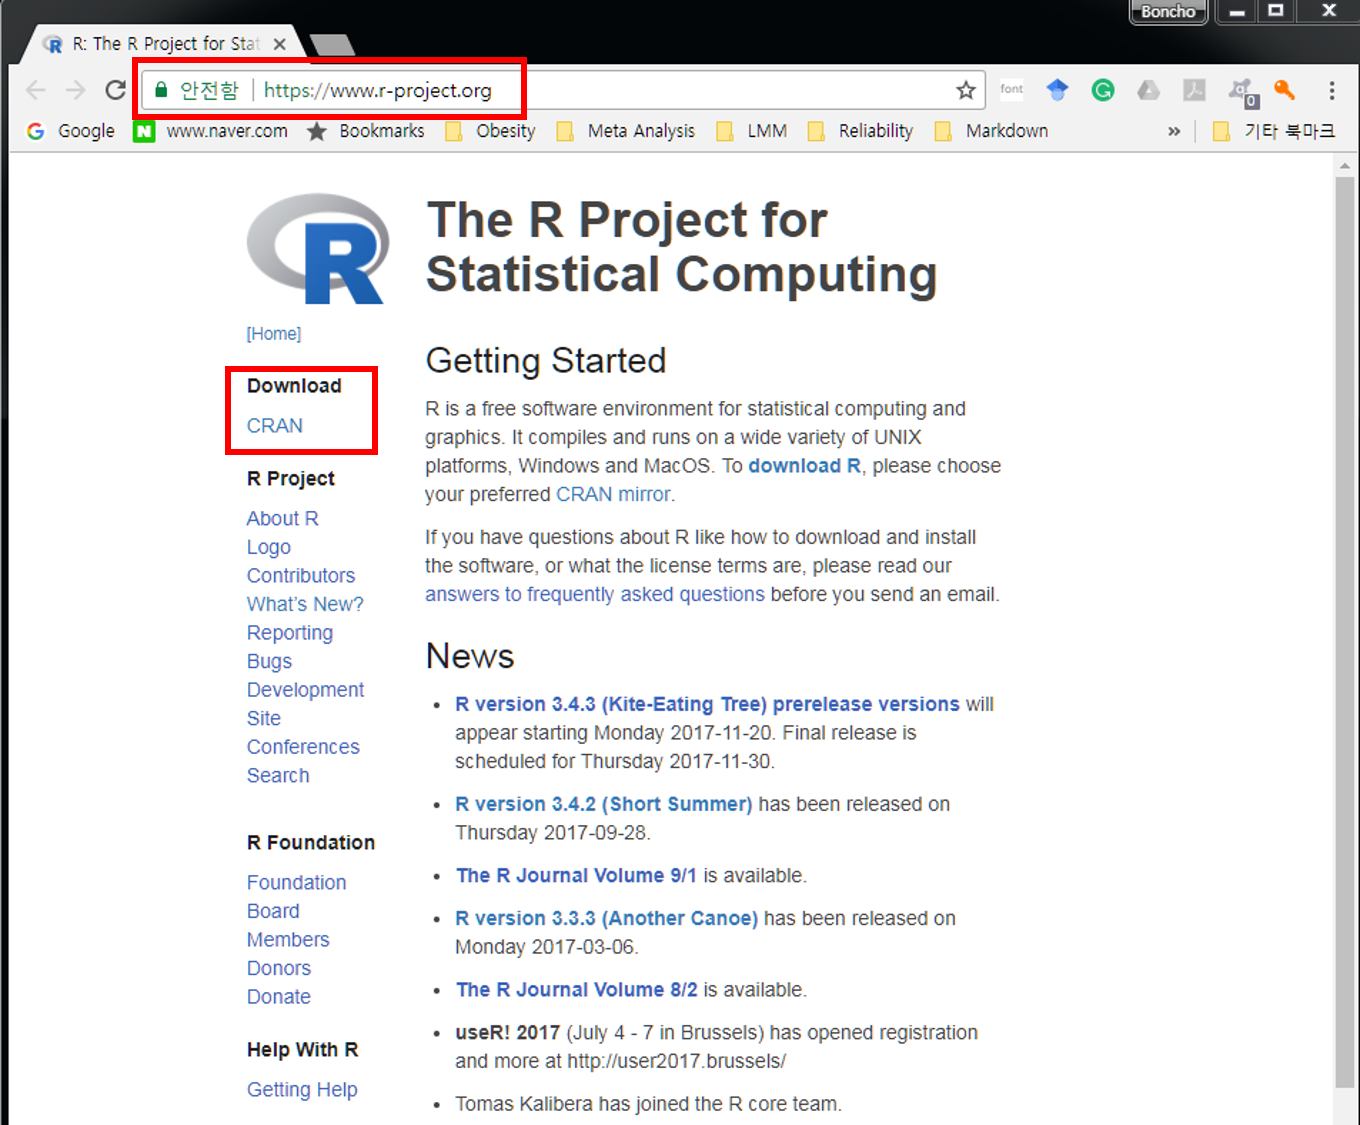
\includegraphics[width=0.9\linewidth]{figures/Rorg-main-add} \end{center}

\normalsize

\begin{enumerate}
\def\labelenumi{\arabic{enumi}.}
\setcounter{enumi}{2}
\tightlist
\item
  클릭 후 연결한 페이지를 스크롤 후 Korea 아래 링크\footnote{해당 링크들은 접속 시점에 따라 변경될 수 있음} 클릭
\end{enumerate}

\footnotesize

\begin{center}
\includegraphics[width=0.9\linewidth]{figures/CRAN-korea-01} \end{center}

\normalsize

\begin{enumerate}
\def\labelenumi{\arabic{enumi}.}
\setcounter{enumi}{3}
\tightlist
\item
  클릭 후 세 가지 운영체제(Linux, Mac OS X, Windowns)에 따른 R 버전 선택 가능\footnote{본 노트는 Windows 버전 설치만 다룸}
\end{enumerate}

\footnotesize

\begin{center}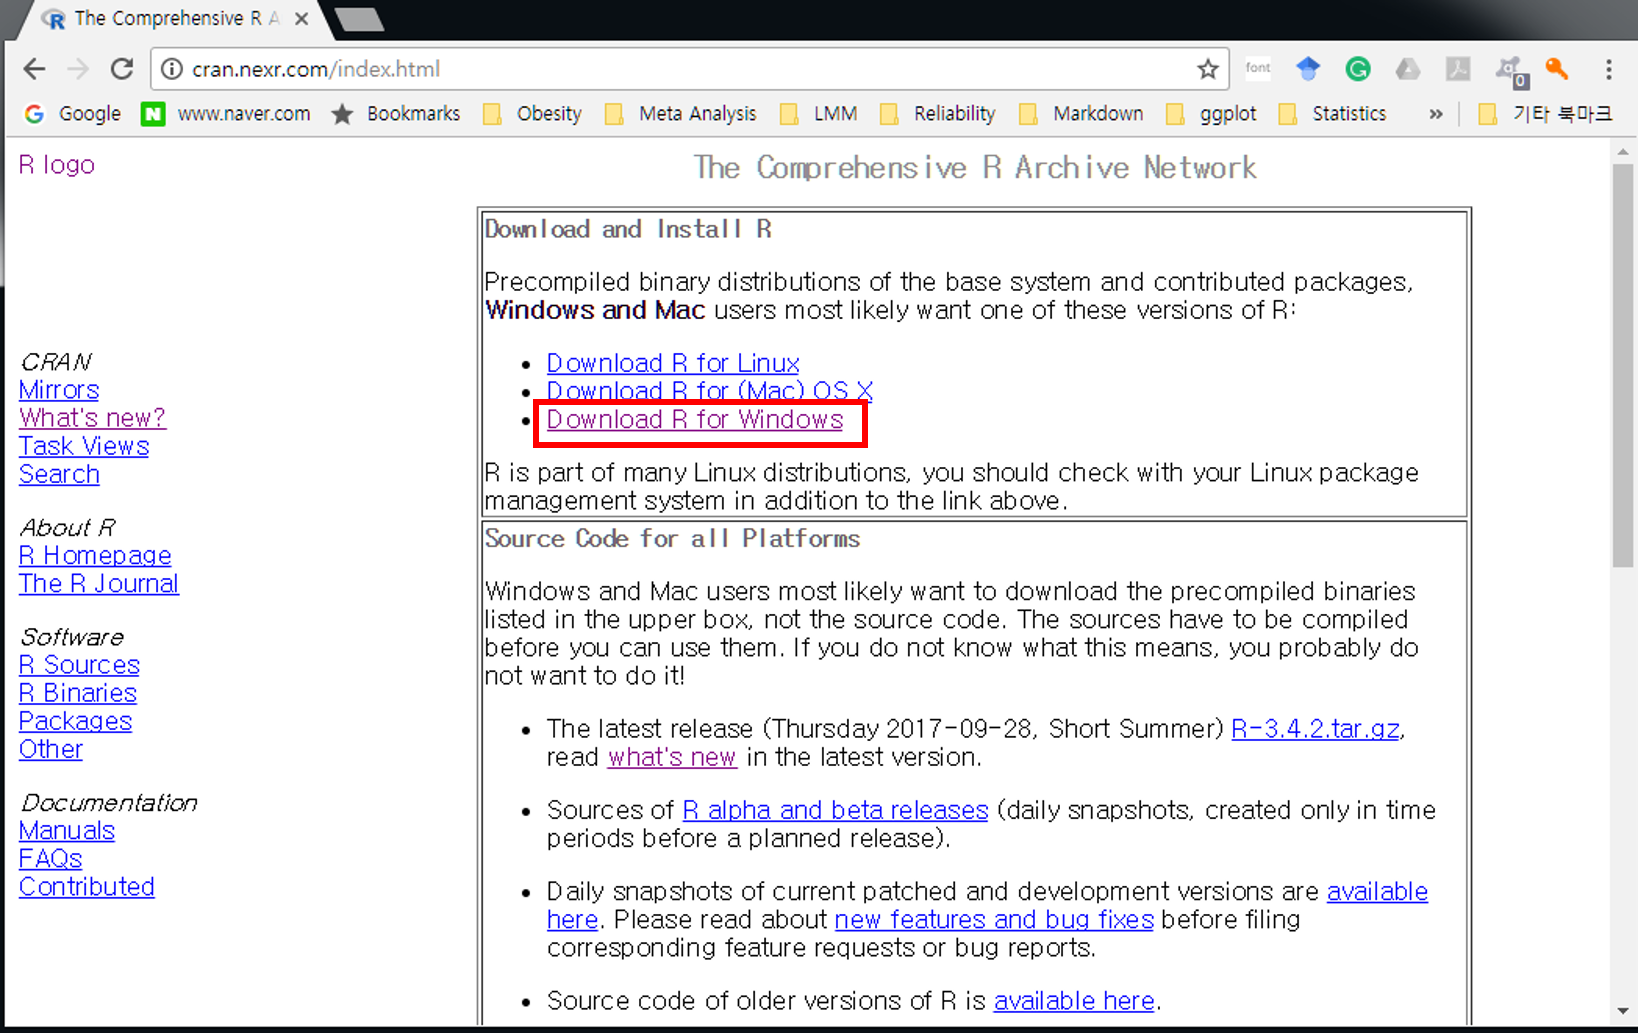
\includegraphics[width=0.9\linewidth]{figures/Rinstall-01} \end{center}

\normalsize

\begin{enumerate}
\def\labelenumi{\arabic{enumi}.}
\setcounter{enumi}{4}
\tightlist
\item
  \textbf{Downloads R for Windows} 링크 클릭하면 다음과 같은 화면으로 이동
\end{enumerate}

\footnotesize

\begin{center}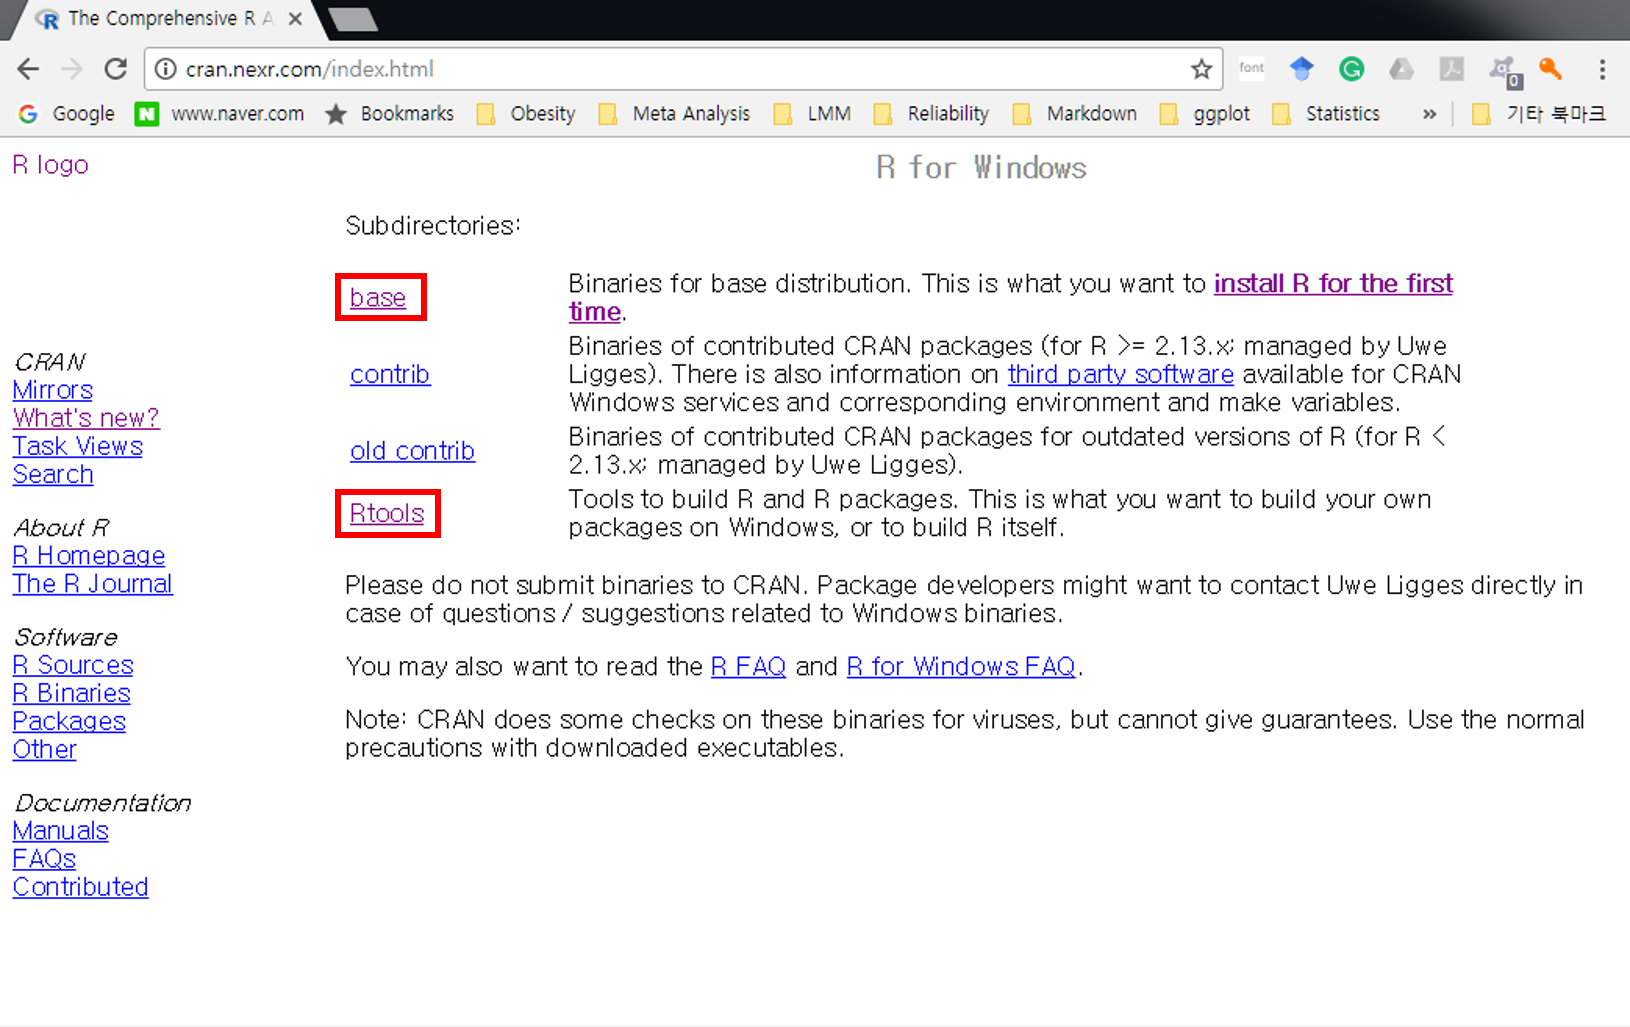
\includegraphics[width=0.9\linewidth]{figures/Rinstall-02} \end{center}

\normalsize

\footnotesize

\BeginKnitrBlock{rmdtip}
다음 하위폴더에 대한 간략 설멍

\begin{itemize}
\tightlist
\item
  \textbf{\texttt{base}}: R 실행 프로그램
\item
  \textbf{\texttt{contrib}}: R package의 바이너리 파일
\item
  \textbf{\texttt{Rtools}}: R package 개발 및 배포를 위한 프로그램
\end{itemize}
\EndKnitrBlock{rmdtip}

\normalsize

\begin{enumerate}
\def\labelenumi{\arabic{enumi}.}
\setcounter{enumi}{5}
\tightlist
\item
  위 화면에서 \textbf{base} 링크 클릭 후 아래 화면에서 \textbf{Downloads R 3.x.x for Windows} 를 클릭 후 설치 파일을 임의의 디렉토리에 저장 및 실행
\end{enumerate}

\footnotesize

\begin{center}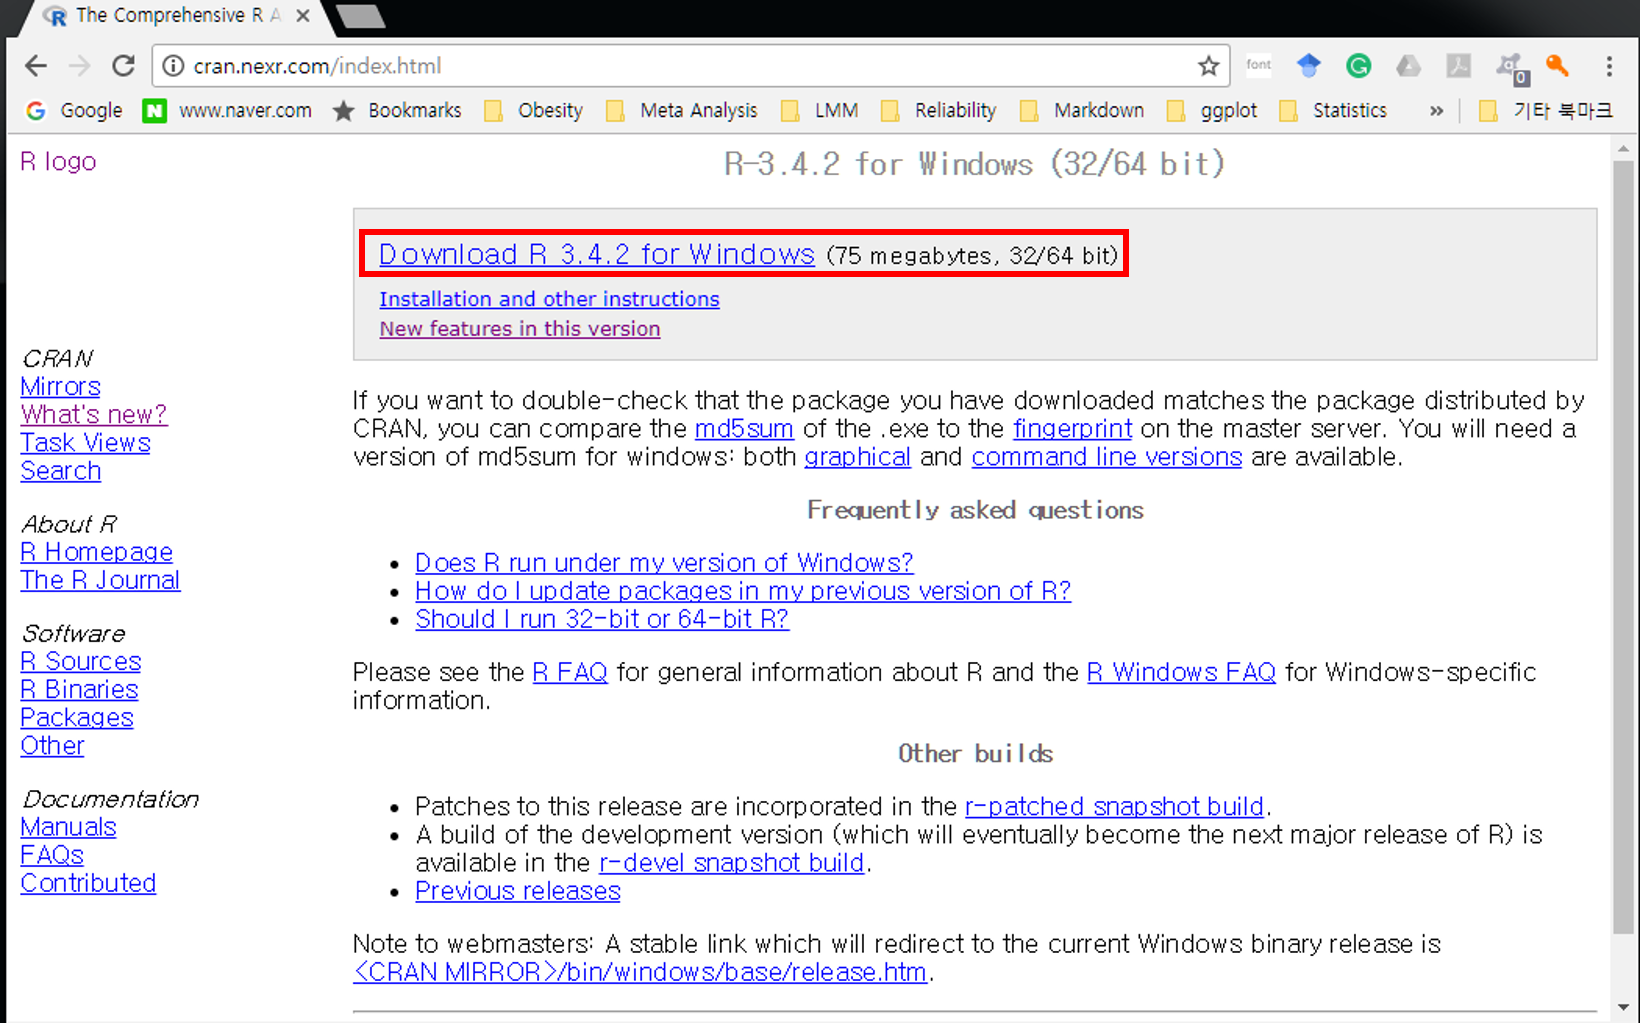
\includegraphics[width=0.9\linewidth]{figures/Rinstall-03} \end{center}

\normalsize

\begin{enumerate}
\def\labelenumi{\arabic{enumi}.}
\setcounter{enumi}{6}
\tightlist
\item
  다운로드한 파일을 실행하면 아래와 같은 대화창이 나타남

  \begin{itemize}
  \tightlist
  \item
    한국어 선택 \(\rightarrow\) 환영 화면에서 {[}다음(N)\textgreater{]} 클릭
  \end{itemize}
\end{enumerate}

\footnotesize

\begin{center}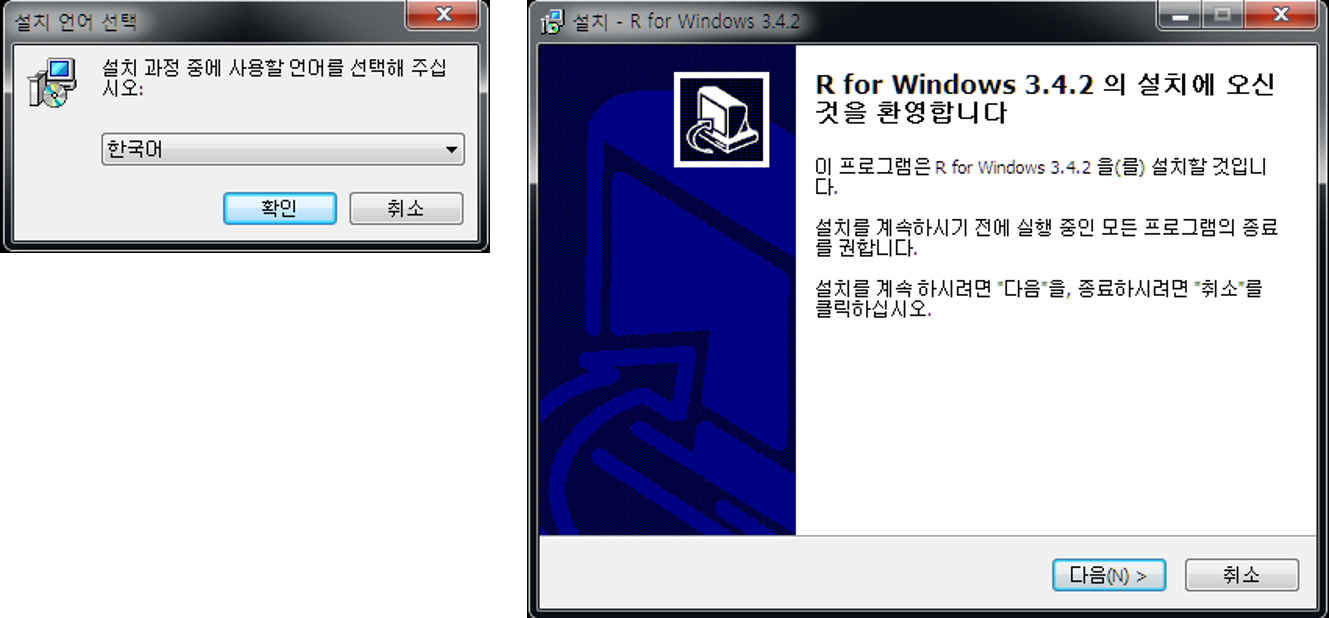
\includegraphics[width=0.9\linewidth]{figures/R-install-F01} \end{center}

\normalsize

\begin{enumerate}
\def\labelenumi{\arabic{enumi}.}
\setcounter{enumi}{7}
\tightlist
\item
  GNU 라이센스에 대한 설명 및 동의 여부({[}다음(N)\textgreater{]}) 클릭
\end{enumerate}

\footnotesize

\begin{center}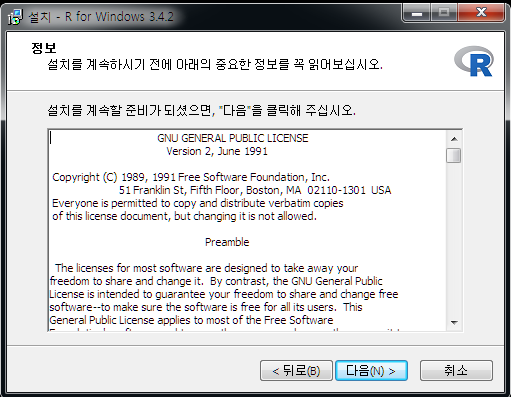
\includegraphics[width=0.9\linewidth]{figures/R-install-F02} \end{center}

\normalsize

\begin{enumerate}
\def\labelenumi{\arabic{enumi}.}
\setcounter{enumi}{8}
\tightlist
\item
  설치 디렉토리 설정 및 구성요소 설지 여부

  \begin{itemize}
  \tightlist
  \item
    원하는 디렉토리 설정(예: \texttt{C:\textbackslash{}R\textbackslash{}R-3.x.x})
  \item
    기본 프로그램(``Core Files''), 32 또는 64 bit 용 설치 파일, R console 한글 번역 모두 체크 뒤 {[}다음(N)\textgreater{]} 클릭
  \end{itemize}
\end{enumerate}

\footnotesize

\begin{center}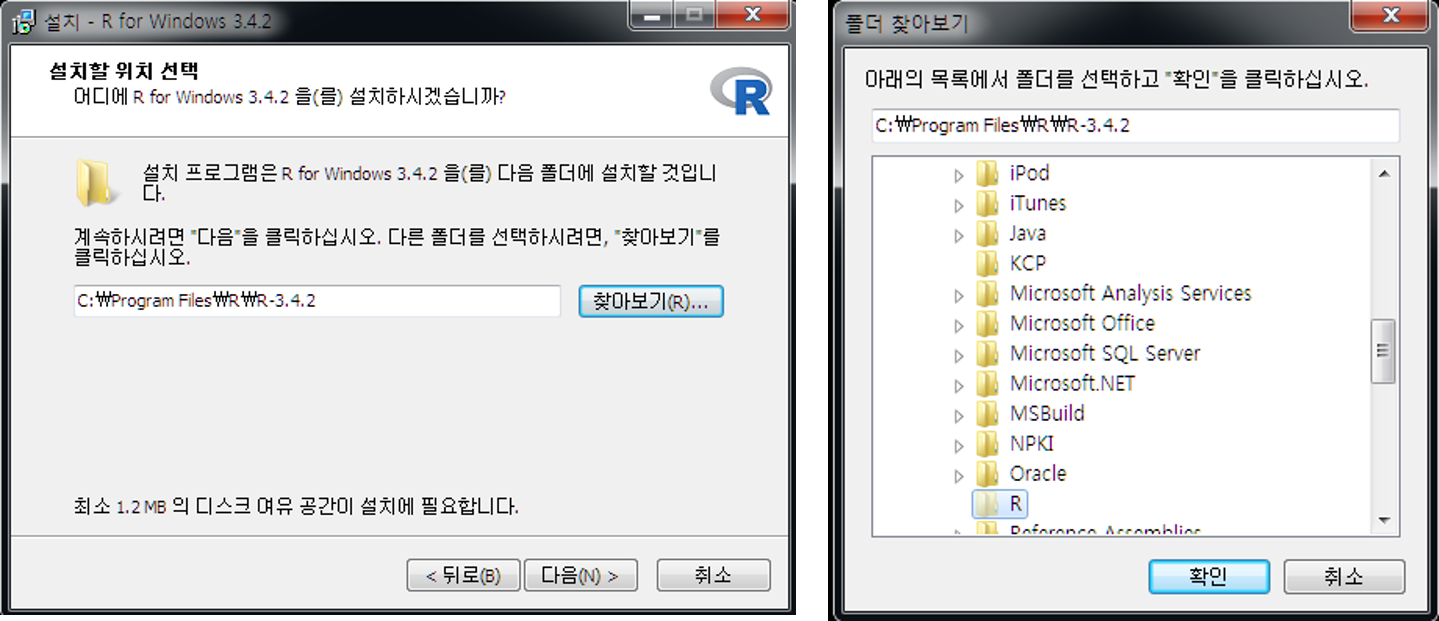
\includegraphics[width=0.9\linewidth]{figures/R-install-F03} \end{center}

\normalsize

\footnotesize

\begin{center}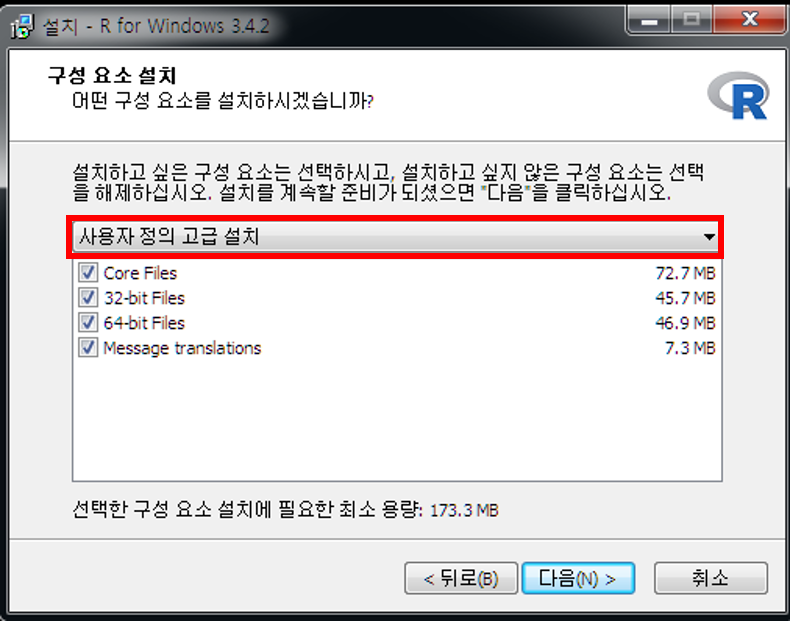
\includegraphics[width=0.9\linewidth]{figures/R-install-F04} \end{center}

\normalsize

\begin{enumerate}
\def\labelenumi{\arabic{enumi}.}
\setcounter{enumi}{9}
\tightlist
\item
  R 스타트업 옵션 지정
\end{enumerate}

\begin{itemize}
\tightlist
\item
  기본값(``No'' check-button)으로도 설치 진행 가능
\item
  본 문서에서는 스타트업 옵션 변경으로 진행
\end{itemize}

\footnotesize

\begin{center}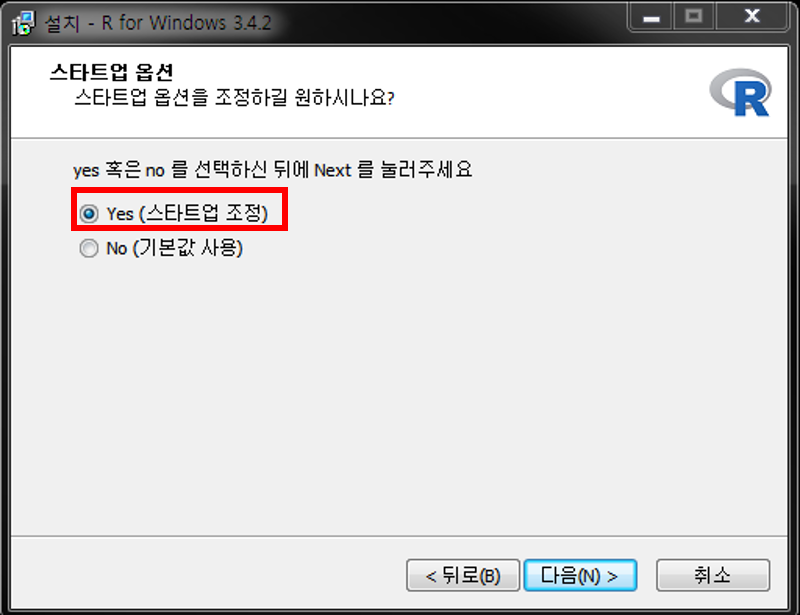
\includegraphics[width=0.9\linewidth]{figures/R-install-F05} \end{center}

\normalsize

\begin{enumerate}
\def\labelenumi{\arabic{enumi}.}
\setcounter{enumi}{10}
\tightlist
\item
  화면표시방식(디스플레이 모드) 설정 변경
\end{enumerate}

\begin{itemize}
\tightlist
\item
  MDI: 한 윈도우 내에서 script 편집창, 출력, 도움말 창 사용
\item
  SDI: 다중 창에서 각각 script 편집창, 출력, 도움말 등을 독립적으로 열기
\end{itemize}

\footnotesize

\begin{center}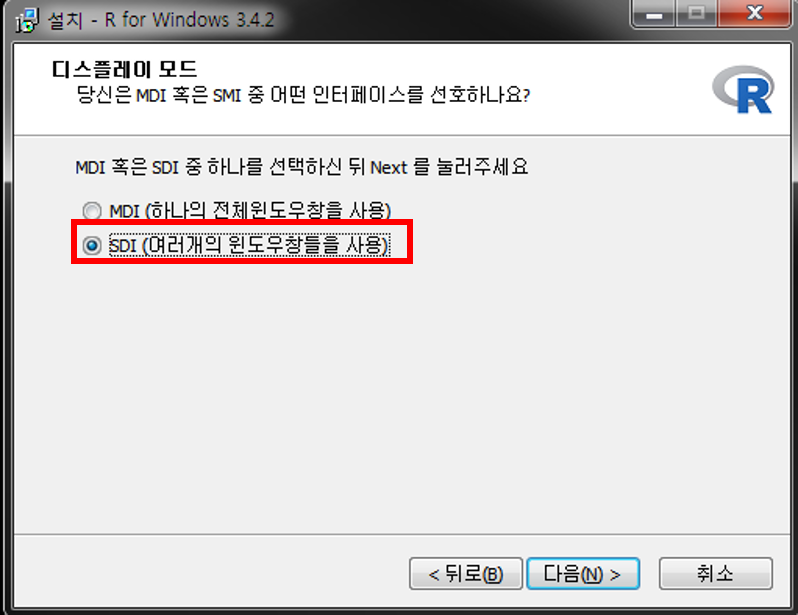
\includegraphics[width=0.9\linewidth]{figures/R-install-F06} \end{center}

\normalsize

\begin{enumerate}
\def\labelenumi{\arabic{enumi}.}
\setcounter{enumi}{11}
\tightlist
\item
  도움말 형식에서 HTML 도움말 기반 선택
\end{enumerate}

\footnotesize

\begin{center}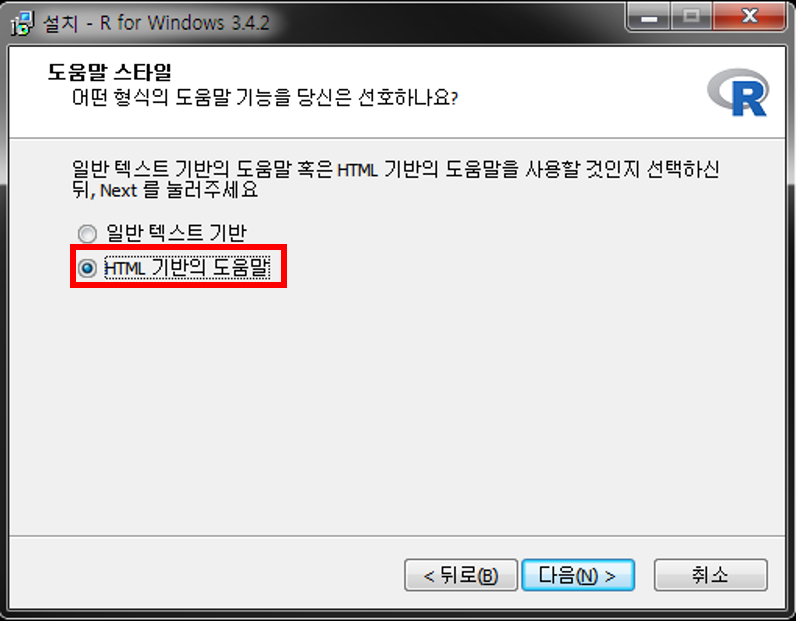
\includegraphics[width=0.9\linewidth]{figures/R-install-F07} \end{center}

\normalsize

\begin{enumerate}
\def\labelenumi{\arabic{enumi}.}
\setcounter{enumi}{12}
\tightlist
\item
  시작메뉴 폴더 선택
\end{enumerate}

\begin{itemize}
\tightlist
\item
  ``바로가기''를 생성할 시작 메뉴 폴더 지정 후 {[}다음(N)\textgreater{]} 클릭 후 설치 진행
\item
  하단 ``시작메뉴 폴더 만들지 않음'' 체크박스 표시 시 시작메뉴에 ``바로가기'' 아이콘이 생성되지 않음(실행에 전혀 지장 없음)
\end{itemize}

\footnotesize

\begin{center}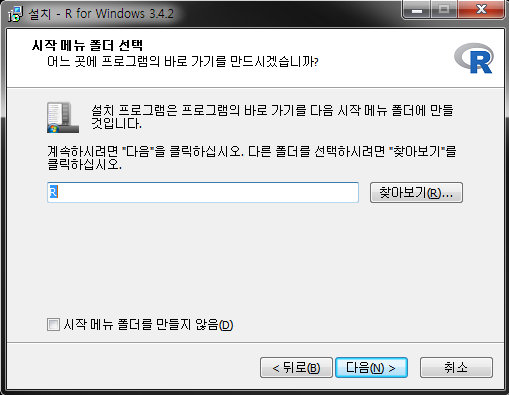
\includegraphics[width=0.9\linewidth]{figures/R-install-F08} \end{center}

\normalsize

\begin{enumerate}
\def\labelenumi{\arabic{enumi}.}
\setcounter{enumi}{13}
\tightlist
\item
  추가 옵션 지정: 바탕화면 아이콘 생성 등 추가적 작업 옵션 체크 후 {[}다음(N)\textgreater{]} 클릭 \(\rightarrow\) 설치 진행
\end{enumerate}

\begin{itemize}
\tightlist
\item
  설치된 R 버전 정보 레지스트리 저장 여부
\item
  \texttt{.Rdata} 확장자를 R 실행파일과 자동 연계
\end{itemize}

\footnotesize

\begin{center}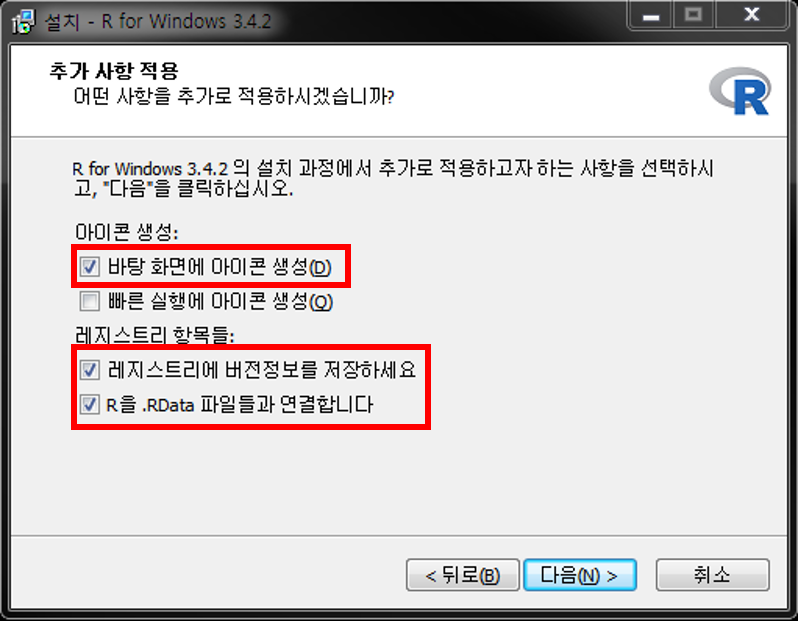
\includegraphics[width=0.9\linewidth]{figures/R-install-F09} \end{center}

\normalsize

\begin{enumerate}
\def\labelenumi{\arabic{enumi}.}
\setcounter{enumi}{14}
\tightlist
\item
  설치 완료 후 바탕화면의 R 아이콘을 더블클릭하면 Rgui가 실행
\end{enumerate}

\footnotesize

\begin{figure}

{\centering 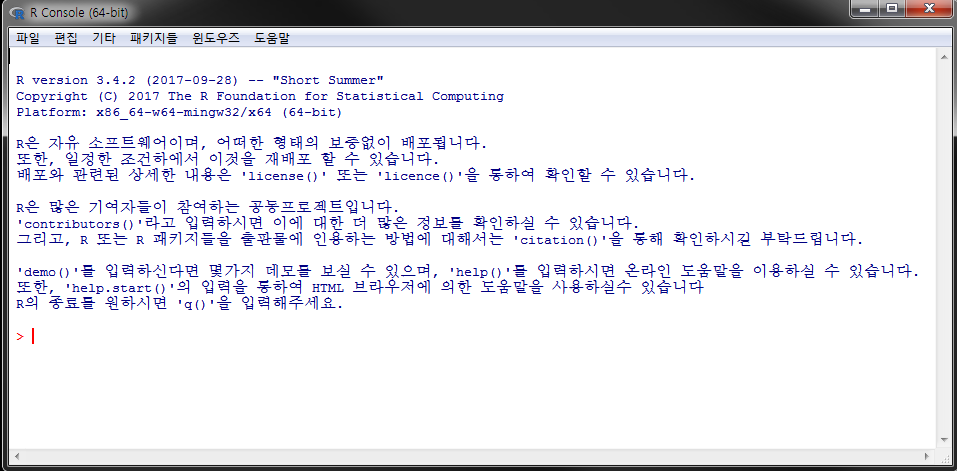
\includegraphics[width=1\linewidth]{figures/Rgui} 

}

\caption{Windows에서 R 실행화면(콘솔 창, SDI 모드)}\label{fig:r-console}
\end{figure}

\normalsize

\hypertarget{r-check}{%
\section{R 시작 및 작동 체크}\label{r-check}}

\BeginKnitrBlock{rmdimportant}
\textbf{실습}: 설치된 R을 실행 후 보이는 R 콘솔(consle) 창에서 명령어를 실행하고 결과 확인
\EndKnitrBlock{rmdimportant}

Figure \ref{fig:r-console} 에서 \texttt{\textgreater{}} 기호는 R의 명령 프롬프트(command prompt) 임

\begin{itemize}
\tightlist
\item
  \(\rightarrow\) 컴퓨터가 사용자 명령을 기다리고 있다는 기호
\end{itemize}

\begin{enumerate}
\def\labelenumi{\arabic{enumi}.}
\tightlist
\item
  현재 R session\footnote{현재 실행되고 있는 R의 작업공간} 정보(R 설치 버전, locale, 로딩 packages) 출력
\end{enumerate}

\footnotesize

\begin{Shaded}
\begin{Highlighting}[]
\CommentTok{# R의 설치 버전 및 현재 설정된 locale(언어, 시간대) 및 로딩된 R package 정보 출력}
\KeywordTok{sessionInfo}\NormalTok{() }
\end{Highlighting}
\end{Shaded}

\begin{verbatim}
R version 3.6.3 (2020-02-29)
Platform: x86_64-w64-mingw32/x64 (64-bit)
Running under: Windows 10 x64 (build 18363)

Matrix products: default

locale:
[1] LC_COLLATE=Korean_Korea.949  LC_CTYPE=Korean_Korea.949   
[3] LC_MONETARY=Korean_Korea.949 LC_NUMERIC=C                
[5] LC_TIME=Korean_Korea.949    

attached base packages:
[1] stats     graphics  grDevices utils     datasets  methods   base     

other attached packages:
[1] knitr_1.28

loaded via a namespace (and not attached):
 [1] compiler_3.6.3  magrittr_1.5    bookdown_0.18.1 htmltools_0.4.0
 [5] tools_3.6.3     yaml_2.2.1      Rcpp_1.0.4      stringi_1.4.6  
 [9] rmarkdown_2.1   stringr_1.4.0   digest_0.6.25   xfun_0.12      
[13] rlang_0.4.5     evaluate_0.14  
\end{verbatim}

\normalsize

\begin{enumerate}
\def\labelenumi{\arabic{enumi}.}
\setcounter{enumi}{1}
\tightlist
\item
  문자열 출력
\end{enumerate}

\footnotesize

\begin{Shaded}
\begin{Highlighting}[]
\CommentTok{#문자열 출력}
\KeywordTok{print}\NormalTok{(}\StringTok{"Hello R"}\NormalTok{) }\CommentTok{#문자열}
\end{Highlighting}
\end{Shaded}

\begin{verbatim}
[1] "Hello R"
\end{verbatim}

\normalsize

\begin{quote}
\texttt{\#} 기호는 주석의 시작을 의미하고 실제로 실행되지 않음 같은 행에서 \texttt{\#} 뒤 내용의 코드 역시 실행되지 않음
\end{quote}

\begin{enumerate}
\def\labelenumi{\arabic{enumi}.}
\setcounter{enumi}{2}
\tightlist
\item
  \texttt{a} 라는 변수에 숫자 9, \texttt{b}라는 변수에 숫자 7를 할당 후 출력
\end{enumerate}

\footnotesize

\begin{Shaded}
\begin{Highlighting}[]
\CommentTok{# 수치형 값(scalar)을 변수에 할당(assign)}
\CommentTok{# 여러 명령어를 한줄에 입력할 때에는 세미콜론(;)으로 구분}
\NormalTok{a =}\StringTok{ }\DecValTok{9}\NormalTok{; b =}\StringTok{ }\DecValTok{7}
\NormalTok{a}
\end{Highlighting}
\end{Shaded}

\begin{verbatim}
[1] 9
\end{verbatim}

\begin{Shaded}
\begin{Highlighting}[]
\NormalTok{b}
\end{Highlighting}
\end{Shaded}

\begin{verbatim}
[1] 7
\end{verbatim}

\normalsize

\begin{enumerate}
\def\labelenumi{\arabic{enumi}.}
\setcounter{enumi}{3}
\tightlist
\item
  변수 \texttt{a}와 \texttt{b}의 사칙연산
\end{enumerate}

\footnotesize

\begin{Shaded}
\begin{Highlighting}[]
\NormalTok{a}\OperatorTok{+}\NormalTok{b; a}\OperatorTok{-}\NormalTok{b; a}\OperatorTok{*}\NormalTok{b; a}\OperatorTok{/}\NormalTok{b}
\end{Highlighting}
\end{Shaded}

\begin{verbatim}
[1] 16
\end{verbatim}

\begin{verbatim}
[1] 2
\end{verbatim}

\begin{verbatim}
[1] 63
\end{verbatim}

\begin{verbatim}
[1] 1.285714
\end{verbatim}

\normalsize

\begin{enumerate}
\def\labelenumi{\arabic{enumi}.}
\setcounter{enumi}{4}
\tightlist
\item
  R 그래픽 맛보기: 정규분포로부터 난수 100개 생성 후 생성된 데이터에 대한 히스토그램 작성
\end{enumerate}

\footnotesize

\begin{Shaded}
\begin{Highlighting}[]
\CommentTok{# 난수 생성 시 값은 매번 달라지기 때문에 seed를 주어 일정값이 생성되도록 고정}
\CommentTok{# "="과 "<-"는 모두 동일한 기능을 가진 할당 연산자임}
\CommentTok{#평균이 0 이고 분산이 1인 정규분포에서 난수 100개 생성}
\KeywordTok{set.seed}\NormalTok{(}\DecValTok{12345}\NormalTok{) }\CommentTok{# random seed 지정}
\NormalTok{x <-}\StringTok{ }\KeywordTok{rnorm}\NormalTok{(}\DecValTok{100}\NormalTok{) }\CommentTok{# 난수 생성}
\KeywordTok{hist}\NormalTok{(x) }\CommentTok{# 히스토그램}
\end{Highlighting}
\end{Shaded}

\begin{figure}

{\centering 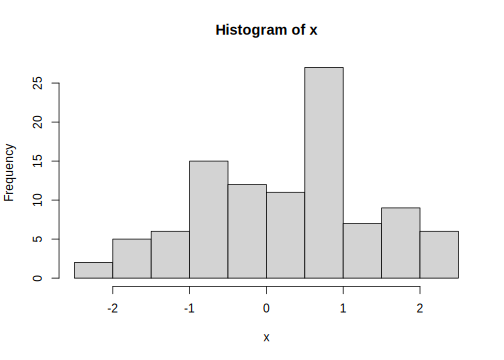
\includegraphics{01-overview_files/figure-latex/check-04-1} 

}

\caption{정규분포 100개의 히스토그램}\label{fig:check-04}
\end{figure}

\normalsize

\footnotesize

\BeginKnitrBlock{rmdtip}
R 명령어 또는 전체 프로그램 소스 실행 시 매우 빈번히 오류가 나타나는데, 이를 해결할 수 있는 가장 좋은 방법은 앞에서 언급한 Google을 이용한 검색 또는 R 설치 시 자체적으로 내장되어 있는 도움말을 참고하는 것이 가장 효율적임.
\EndKnitrBlock{rmdtip}

\normalsize

\footnotesize

\begin{table}[H]

\caption{\label{tab:tab-help}R help 관련 명령어 리스트}
\centering
\fontsize{10}{12}\selectfont
\begin{tabular}[t]{l>{\raggedright\arraybackslash}p{5cm}l}
\toprule
도움말 보기 명령어 & 설명 & 사용법\\
\midrule
\rowcolor{gray!6}  `help` 또는 `?` & 도움말 시스템 호출 & `help(함수명)`\\
`help.search` 또는 `??` & 주어진 문자열을 포함한 문서 검색 & `help.search(pattern)`\\
\rowcolor{gray!6}  `example` & topic의 도움말 페이지에 있는 examples section 실행 & `example(함수명)`\\
`vignette` & topic의 pdf 또는 html 레퍼런스 메뉴얼 불러오기 & `vignette(패키지명 또는 패턴)`\\
\bottomrule
\end{tabular}
\end{table}

\normalsize

\footnotesize

\BeginKnitrBlock{rmdtip}
\textbf{Vignette} 의 활용

\begin{itemize}
\tightlist
\item
  \texttt{vignette()}에서 제공하는 문서는 데이터를 기반으로 사용하고자 하는 패키지의 실제 활용 예시를 작성한 문서이기 때문에 초보자들이 R 패키지 활용에 대한 접근성을 높혀줌.
\item
  \texttt{browseVignettes()} 명령어를 통해 vignette을 제공하는 R 패키지 및 해당 vignette 문서 확인 가능
\end{itemize}
\EndKnitrBlock{rmdtip}

\normalsize

\hypertarget{rconsle-script}{%
\section{R script 편집기 사용}\label{rconsle-script}}

\BeginKnitrBlock{rmdimportant}
\textbf{실습}: R 설치 후 Rgui 에서 제공하는 편집기(R editor)에 명령어를 입력하고 실행
\EndKnitrBlock{rmdimportant}

설치된 R을 실행 후 상단 pull-down 메뉴에서 {[}\textbf{File}{]} \(\rightarrow\) {[}\textbf{새 스크립트}{]}를 선택하면 아래 그림과 같이 편집창(R 인스톨 시 SDI 옵션 기준)이 나타남

\footnotesize

\begin{center}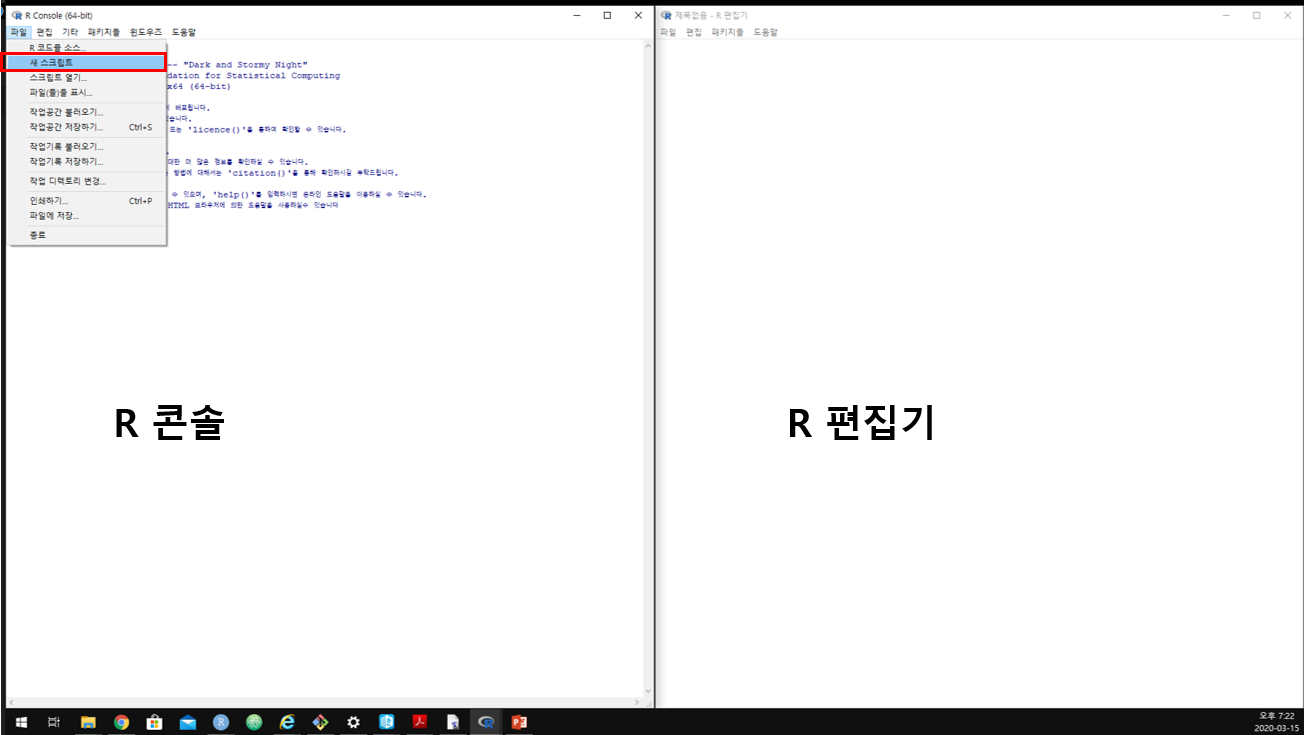
\includegraphics[width=1\linewidth]{figures/r-console-edit} \end{center}

\normalsize

편집기 창에 다음 명령어 입력

\footnotesize

\begin{Shaded}
\begin{Highlighting}[]
\CommentTok{# R에 내장된 cars 데이터셋 불러오기 cars dataset에 포함된 변수들의 기초통계량}
\CommentTok{# 출력 2차원 산점도}
\KeywordTok{data}\NormalTok{(cars)}
\KeywordTok{help}\NormalTok{(cars)  }\CommentTok{# cars 데이터셋에 대한 설명 help 창에 출력}
\KeywordTok{head}\NormalTok{(cars)  }\CommentTok{# cars 데이터셋 처음 6개 행 데이터 출력}
\KeywordTok{summary}\NormalTok{(cars)  }\CommentTok{# cars 데이터셋 요약}
\KeywordTok{plot}\NormalTok{(cars)  }\CommentTok{# 변수가 2개인 경우 산점도 출력}
\end{Highlighting}
\end{Shaded}

\normalsize

\begin{itemize}
\tightlist
\item
  편집창에서 한 줄을 실행시키려면 명령어가 입력된 줄에서 \textbf{{[}Ctrl{]}} + \textbf{{[}R{]}} 입력
\item
  편집창에 입력한 모든 명령어를 실행시키려면 모든 줄을 선택(마우스 또는 {[}Shift{]} + \(\downarrow\))
\end{itemize}

\footnotesize

\begin{verbatim}
  speed dist
1     4    2
2     4   10
3     7    4
4     7   22
5     8   16
6     9   10
\end{verbatim}

\begin{verbatim}
     speed           dist       
 Min.   : 4.0   Min.   :  2.00  
 1st Qu.:12.0   1st Qu.: 26.00  
 Median :15.0   Median : 36.00  
 Mean   :15.4   Mean   : 42.98  
 3rd Qu.:19.0   3rd Qu.: 56.00  
 Max.   :25.0   Max.   :120.00  
\end{verbatim}

\begin{figure}
\centering
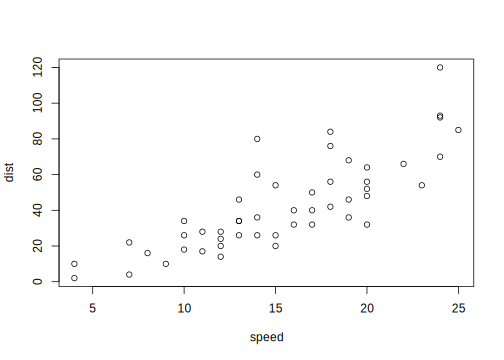
\includegraphics{01-overview_files/figure-latex/check-edit-out-1.pdf}
\caption{\label{fig:check-edit-out}cars 데이터셋의 speed와 dist 간 2차원 산점도: speed는 자동차 속도(mph)이고 dist는 해당 속도에서 브레이크를 밟았을 때 멈출 때 까지 걸린 거리(ft)를 나타냄.}
\end{figure}

\normalsize

\begin{itemize}
\tightlist
\item
  R은 명령어를 입력하고 실행결과를 확인하는 대화형(interpreter) 방식
\item
  콘솔창에서 \(\uparrow\)/\(\downarrow\)를 누르면 이전/이후 실행 명령 기록 확인 가능
\item
  여러 줄 이상 R 명령어라든가 반복적, 장기간 작업을 수행해야 할 경우 R 명령어로 구성된 스크립트 작성 후 일괄 실행하는 것이 일반적
\item
  여러 다중 명령 코딩 시 콘솔창에 직접 입력하는 것은 비효율적이므로 스크립트 에디터를 사용
\item
  위 예시처럼 R 에디터 사용할 수 있으나 가독성 및 코딩 효율이 떨어짐
\item
  과거 많이 사용됐던 R 에디터: \href{http://www.winedt.com}{WinEdt}, \href{https://sourceforge.net/projects/tinn-r/}{Tinn-R}, \href{http://www.vim.org/scripts/script.php?script_id=2628}{Vim}
\item
  현재 가장 범용적 R 에디터: \textbf{Rstudio}
\end{itemize}

\hypertarget{r-studio}{%
\section{RStudio}\label{r-studio}}

\begin{itemize}
\tightlist
\item
  \href{https://rstudio.com/}{RStudio}: R 통합 분석/개발 환경(integrated development environment, IDE)으로 현재 가장 대중적으로 사용되고 있는 R 사용 환경
\item
  명령 곤솔 외 파일 편집, 데이터 객체, 명령 기록(.history), 그래프 등에 쉽게 접근 가능
\item
  RStudio 독자적인 개발 환경 제공: Rmarkdown, Rnotebook, Shiny Web Application 등 다양한 R 환경을 제공
\item
  버전관리(git, subversion)를 통해 project 관리 가능
\item
  \textbf{무료} 및 유료 소프트웨어 제공
\end{itemize}

\hypertarget{rstudio-install}{%
\subsection{RStudio 설치하기}\label{rstudio-install}}

\begin{enumerate}
\def\labelenumi{\arabic{enumi}.}
\tightlist
\item
  웹 브라우저를 통해 \url{https://rstudio.com} 접속 후 상단 \href{https://rstudio.com/products/rstudio/download/}{DOWNLOAD} 링크 클릭
\end{enumerate}

\footnotesize

\begin{center}
\includegraphics[width=0.8\linewidth]{figures/rstudio-homepage} \end{center}

\normalsize

\begin{enumerate}
\def\labelenumi{\arabic{enumi}.}
\setcounter{enumi}{1}
\item
  Desktop 또는 Server 버전 중 택일

  \begin{itemize}
  \tightlist
  \item
    서버용 설치를 위해서는 Server 클릭 \(\rightarrow\) 소규모 자료 분석용으로는 불필요
  \item
    여기서는 \textbf{Desktop} 버전 선택 후 다음 링크로 이동
  \end{itemize}
\end{enumerate}

\footnotesize

\begin{center}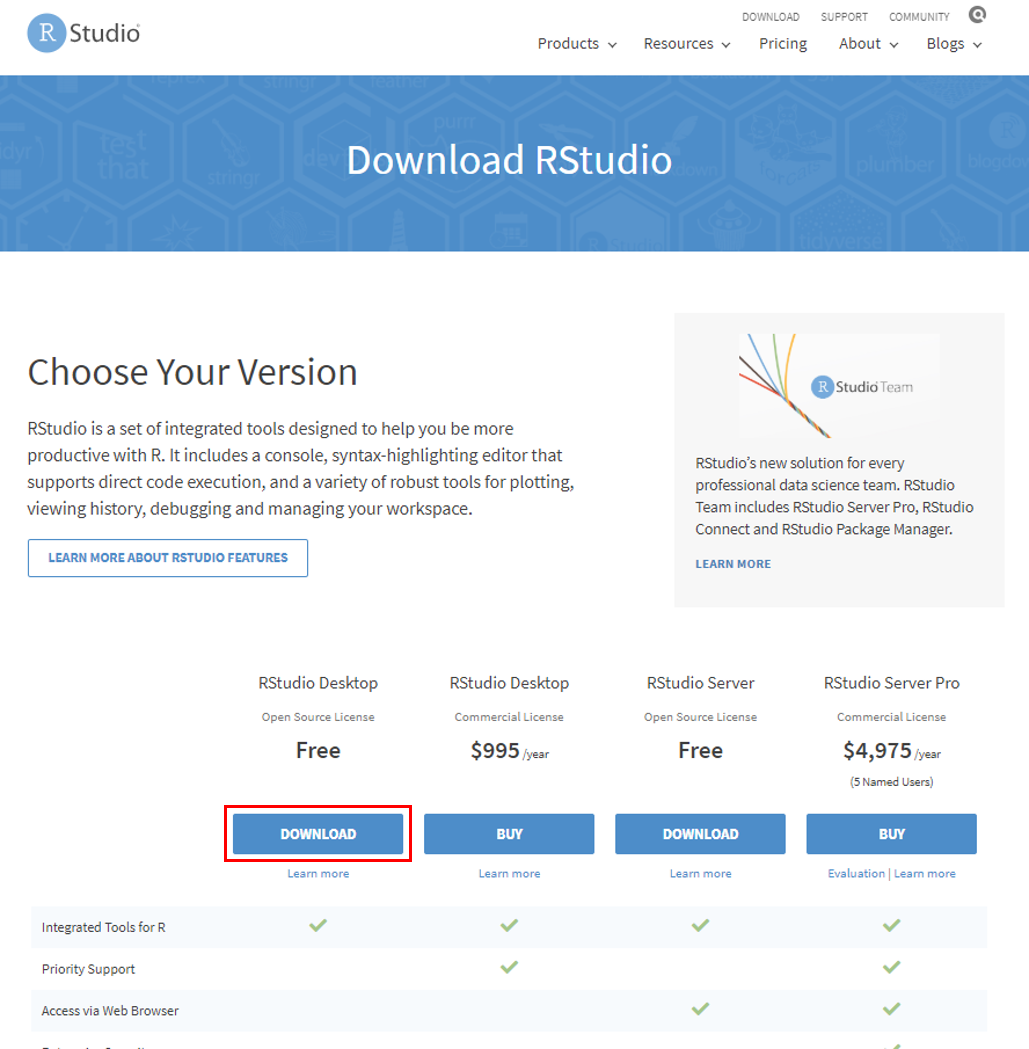
\includegraphics[width=0.7\linewidth]{figures/rstudio-download} \end{center}

\normalsize

\begin{enumerate}
\def\labelenumi{\arabic{enumi}.}
\setcounter{enumi}{2}
\tightlist
\item
  운영체제에 맞는 Rstudio installer 다운로드(여기서는 Windows 버전 다운로드)
\end{enumerate}

\footnotesize

\begin{center}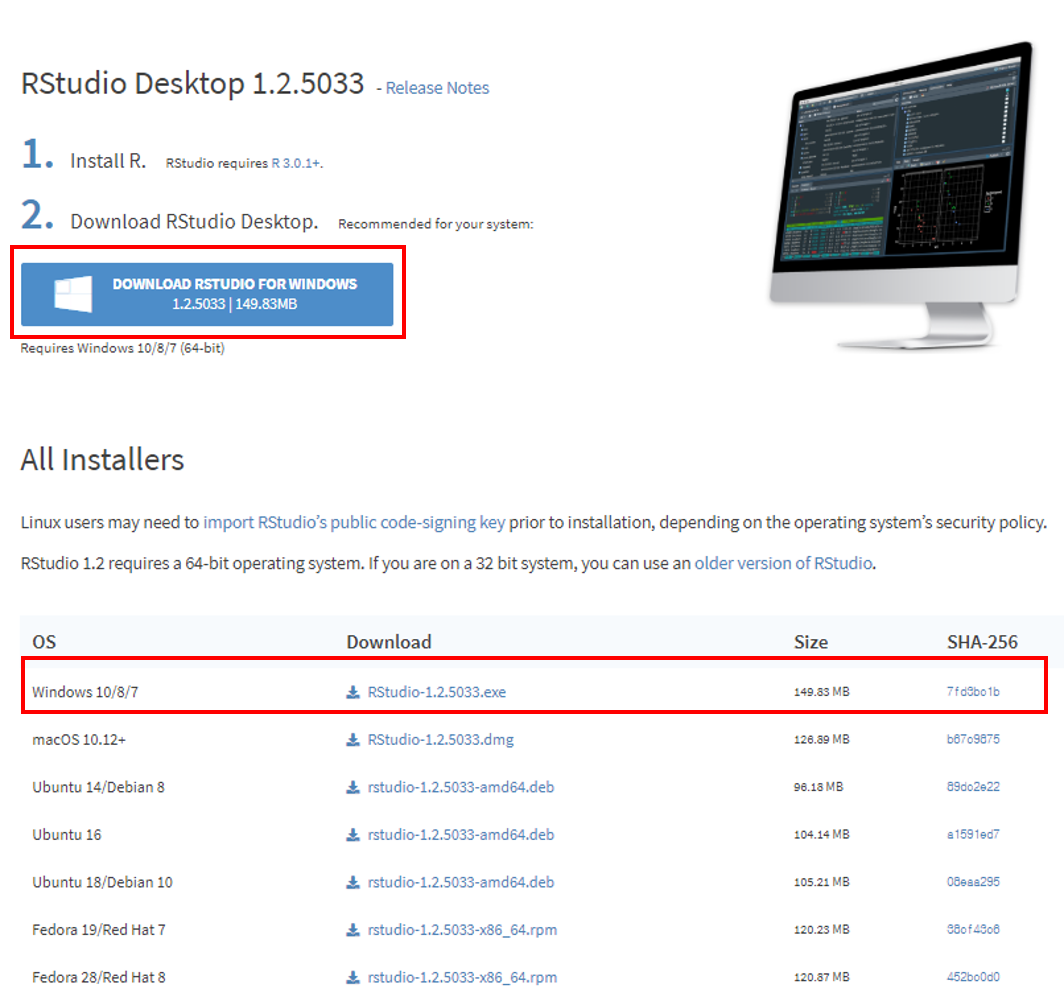
\includegraphics[width=0.6\linewidth]{figures/r-studio-download-02} \end{center}

\normalsize

\begin{enumerate}
\def\labelenumi{\arabic{enumi}.}
\setcounter{enumi}{3}
\tightlist
\item
  RStudio installer 다운로드 시 파일이 저장된 폴더에서 보통 \texttt{RStudio-xx.xx.xxx.exe} 형식의 파일명 확인

  \begin{itemize}
  \tightlist
  \item
    더블 클릭 후 실행
  \item
    \textbf{{[}다음\textgreater{]}} 몇 번 클릭 후 설치 종료
  \end{itemize}
\end{enumerate}

\footnotesize

\begin{center}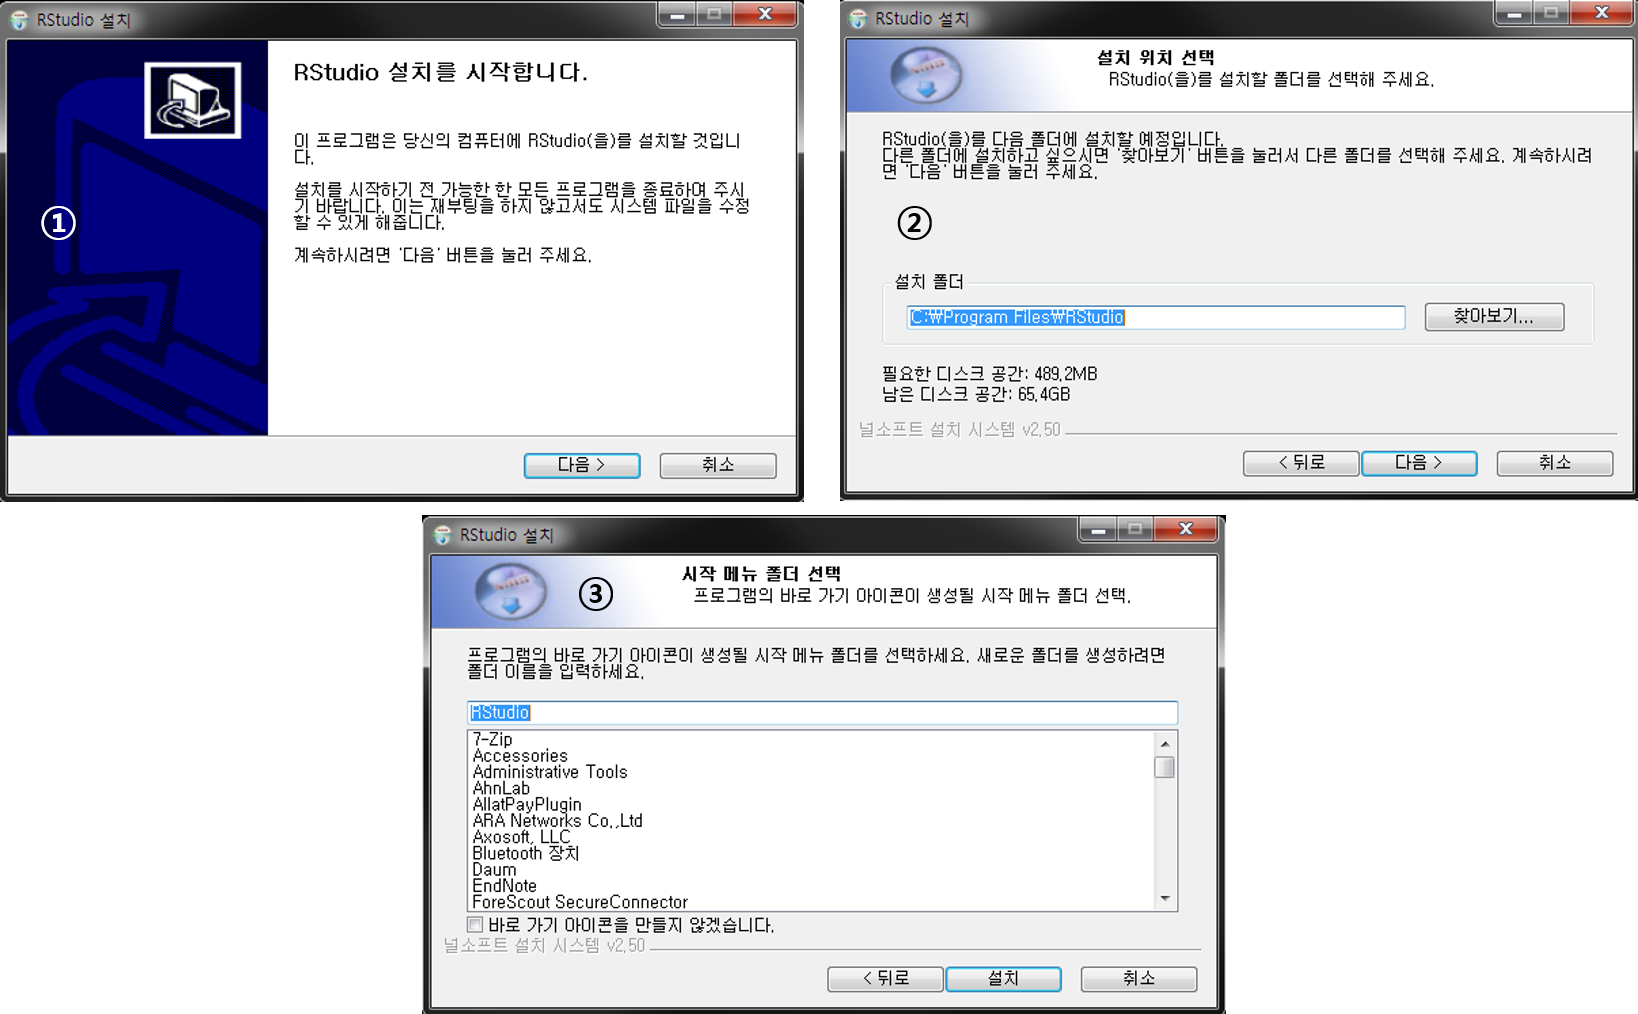
\includegraphics{figures/Rstudio-installer} \end{center}

\normalsize

\begin{enumerate}
\def\labelenumi{\arabic{enumi}.}
\setcounter{enumi}{4}
\tightlist
\item
  바탕화면 혹은 시작 프로그램에 새로 설치된 RStudio 아이콘 클릭 후 아래와 같은 프로그램 창이 나타나면 설치 성공
\end{enumerate}

\footnotesize

\begin{center}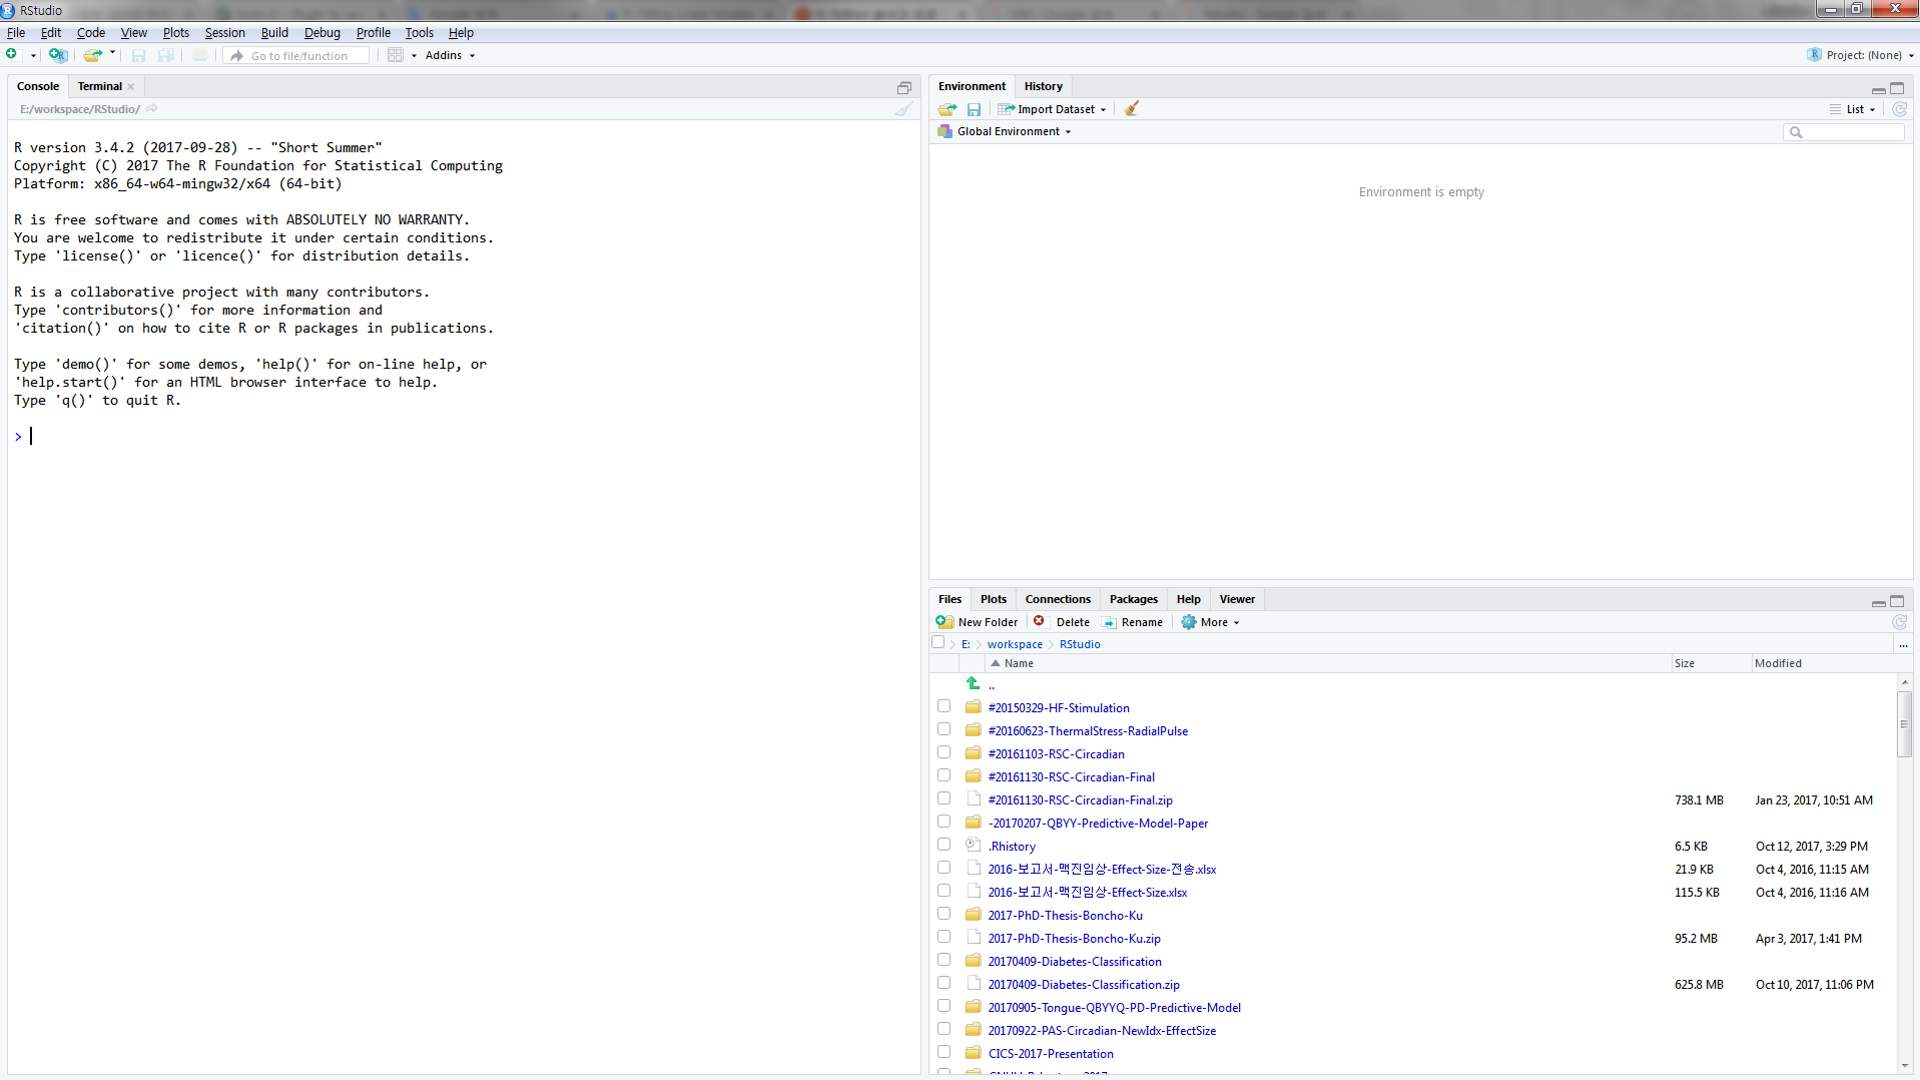
\includegraphics[width=0.8\linewidth]{figures/Rstudio-init} \end{center}

\normalsize

\hypertarget{rstudio-component}{%
\subsection{RStudio IDE 화면 구성}\label{rstudio-component}}

RStudio는 아래 그림과 같이 4개 창으로 구성\footnote{각 창의 위치는 세팅 구성에 따라 달라질 수 있음. 창 구성 방법은 RStudio 환경 옵션 설정에서 설명함.}

\footnotesize

\begin{figure}

{\centering 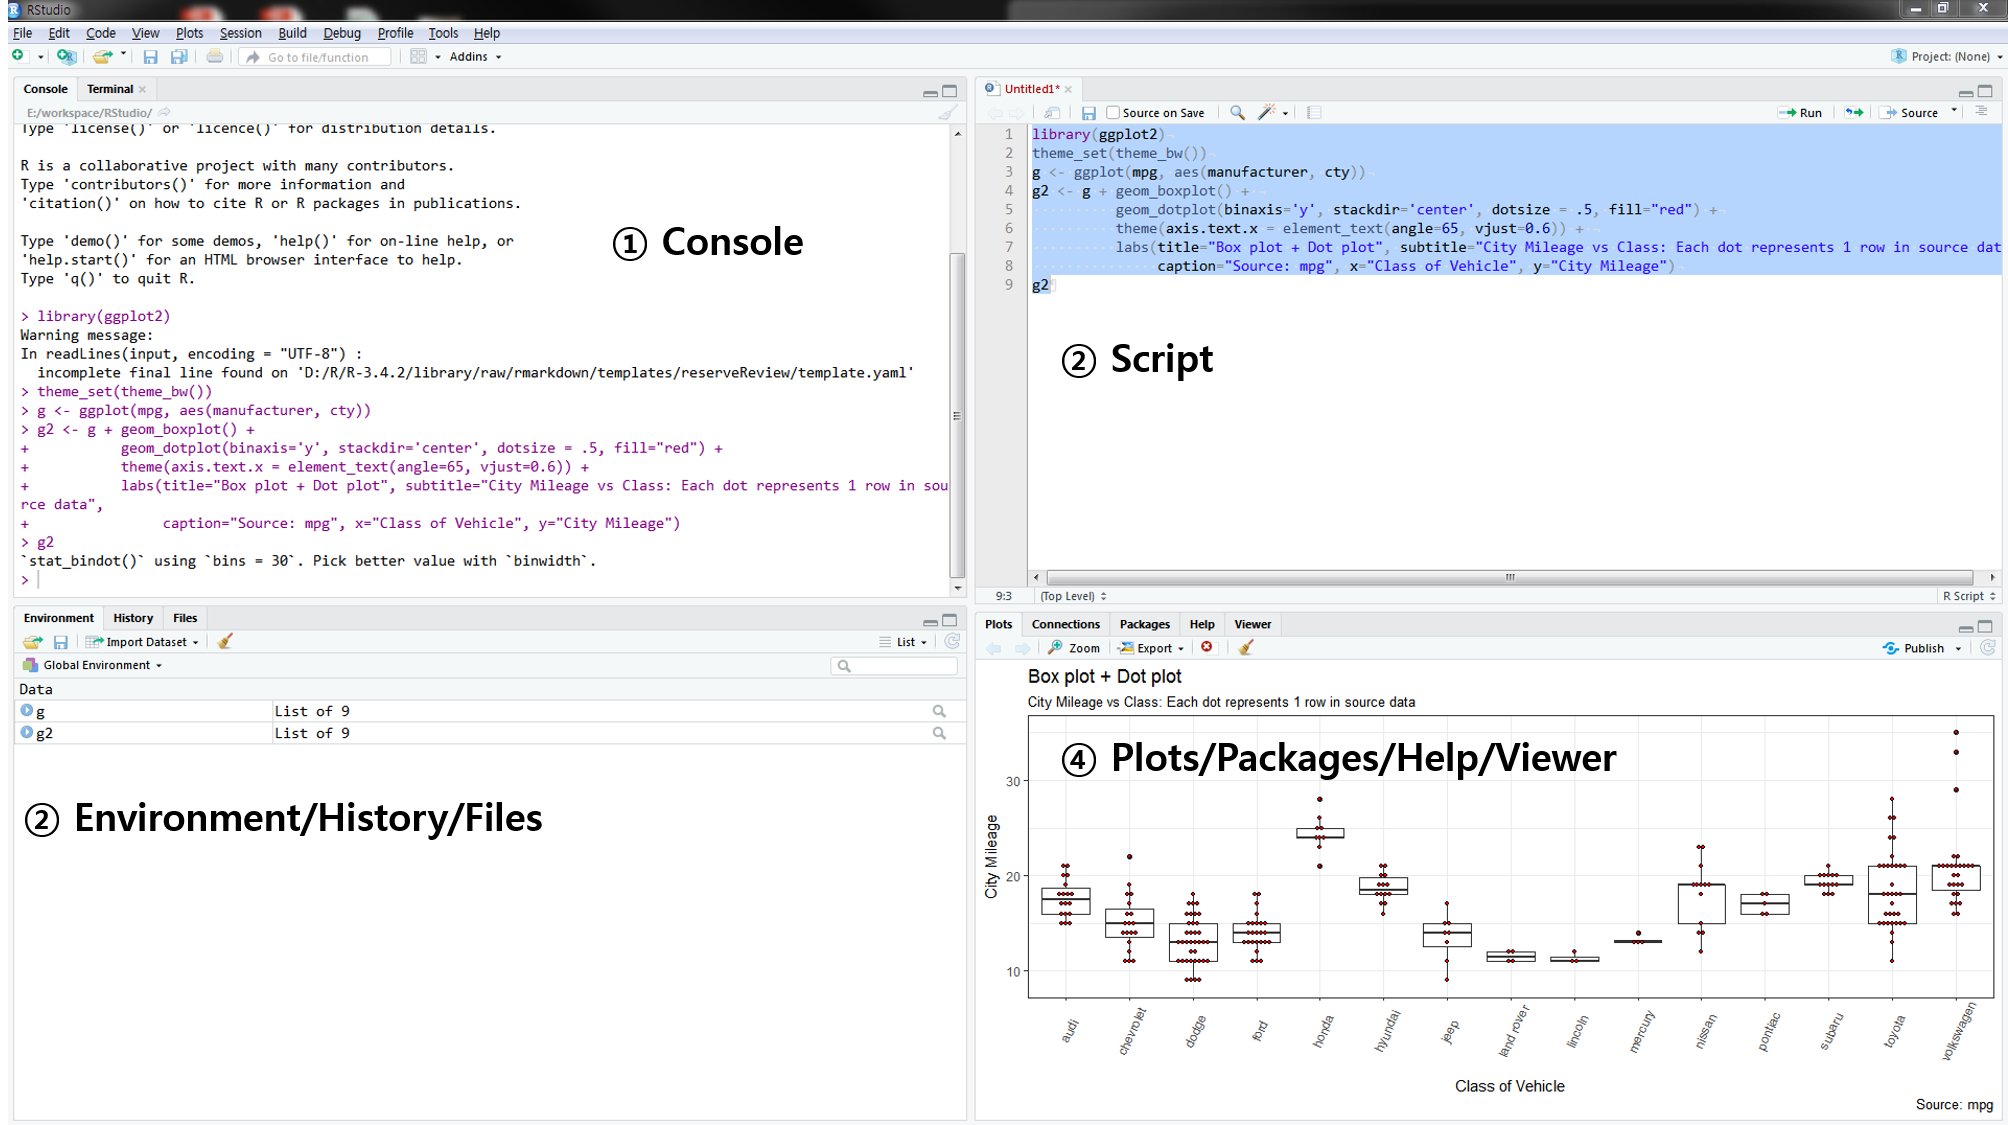
\includegraphics[width=0.9\linewidth]{figures/Rstudio-cap1} 

}

\caption{RStudio 화면구성: 우하단 그림은 http://r-statistics.co/Top50-Ggplot2-Visualizations-MasterList-R-Code.html 에서 발췌}\label{fig:rstudio-windows}
\end{figure}

\normalsize

\textbf{1. 콘솔(console)}

\begin{itemize}
\tightlist
\item
  R 명령어 실행공간(RGui, 정확하게는 R 설치 디렉토리에서 ``\textasciitilde/R/R.x.x/bin/x64/Rterm.exe'' 가 구동되고 있는 공간)
\item
  R script 또는 콘솔 창에서 작성한 명령어(프로그램) 실행 및 그 결과 출력
\item
  경고, 에러/로그 등의 메세지 확인
\end{itemize}

\footnotesize

\begin{figure}

{\centering 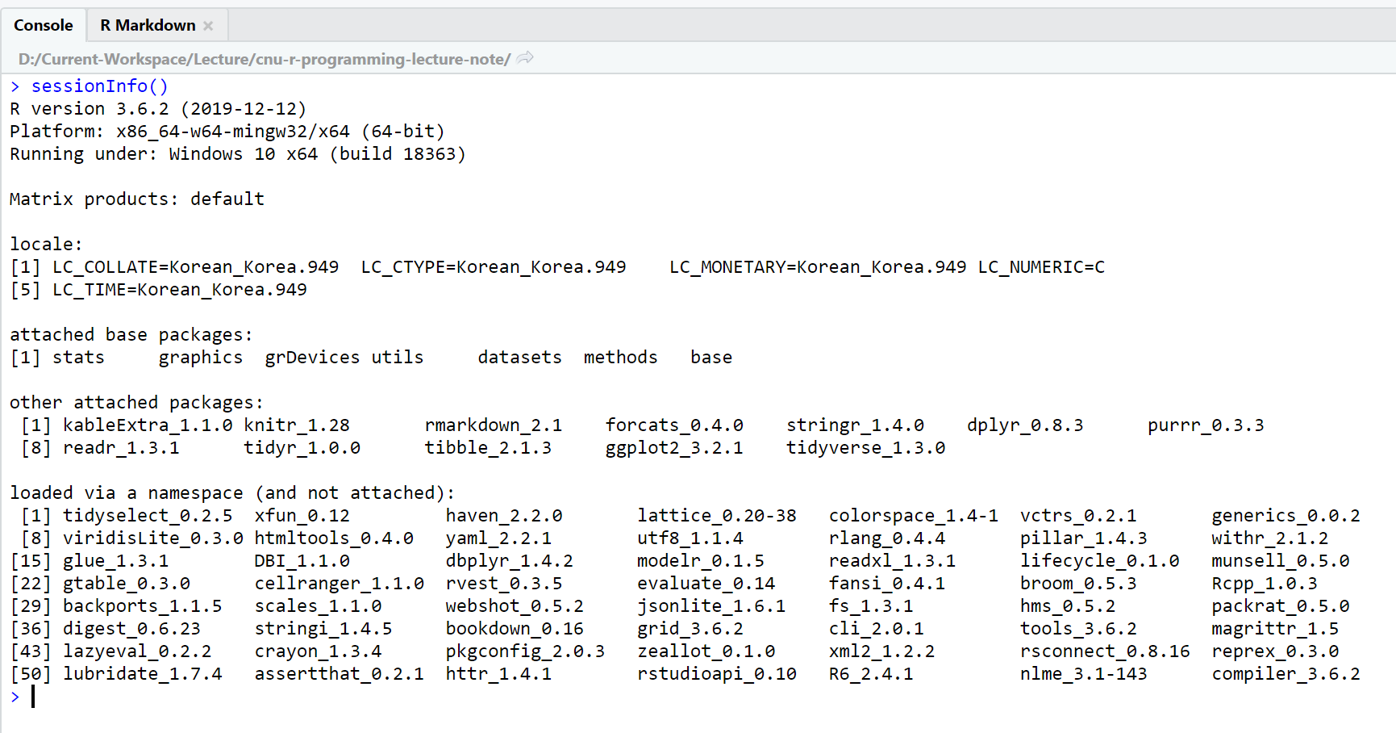
\includegraphics[width=0.8\linewidth]{figures/rstudio-console} 

}

\caption{RStudio 콘솔창에서 명령어 실행 후 출력결과 화면}\label{fig:rstudio-console}
\end{figure}

\normalsize

\textbf{2. 스크립트(script)} (Figure \ref{fig:rstudio-new-script})

\begin{itemize}
\tightlist
\item
  R 명령어 입력 공간으로 일괄처리(batch processing) 가능
\item
  새로운 스크립트 창 열기

  \begin{itemize}
  \tightlist
  \item
    아래 그림과 같이 pull-down 메뉴 좌측 상단 아이콘 클릭 후 {[}R script{]} 선택
  \item
    \texttt{{[}File{]}} \(\rightarrow\) \texttt{{[}New\ File{]}} \(\rightarrow\) \texttt{{[}R\ Script{]}} 선택
  \item
    단축 키: \texttt{{[}Ctrl{]}\ +\ {[}Shift{]}\ +\ {[}N{]}}
  \end{itemize}
\item
  일괄 명령어 처리를 위한 RStudio 제공 단축 키

  \begin{itemize}
  \tightlist
  \item
    \texttt{{[}Ctrl{]}\ +\ {[}Enter{]}}: 선택한 블럭 내 명령어 실행
  \item
    \texttt{{[}Alt{]}\ +\ {[}Enter{]}}: 선택 없이 커서가 위치한 라인의 명령어 실행
  \end{itemize}
\item
  R 스크립트 이외 R Markdown, R Notebook, Shiny web application 등 새 문서의 목적에 따라 다양한 종류의 소스 파일 생성 가능
\item
  저장된 R 스크립트 파일은 \texttt{파일명.R}로 저장됨
\item
  파일 실행 방법

  \begin{itemize}
  \tightlist
  \item
    실행하고자 하는 파일을 읽은 후(\texttt{{[}File{]}} \(\rightarrow\) \texttt{{[}Open\ File{]}} + 파일명 선택 또는 \texttt{파일명.R} 더블 클릭) 입력된 모든 라인을 선택한 뒤 \texttt{{[}Ctrl{]}\ +\ {[}Enter{]}}
  \item
    파일 읽은 후 \texttt{{[}Ctrl{]}\ +\ {[}Shift{]}\ +\ {[}S{]}} (현재 열려있는 \texttt{*.R} 파일에 대해) 또는 \texttt{{[}Ctrl{]}\ +\ {[}Shift{]}\ +\ {[}Enter{]}}
  \end{itemize}
\end{itemize}

\footnotesize

\begin{figure}

{\centering 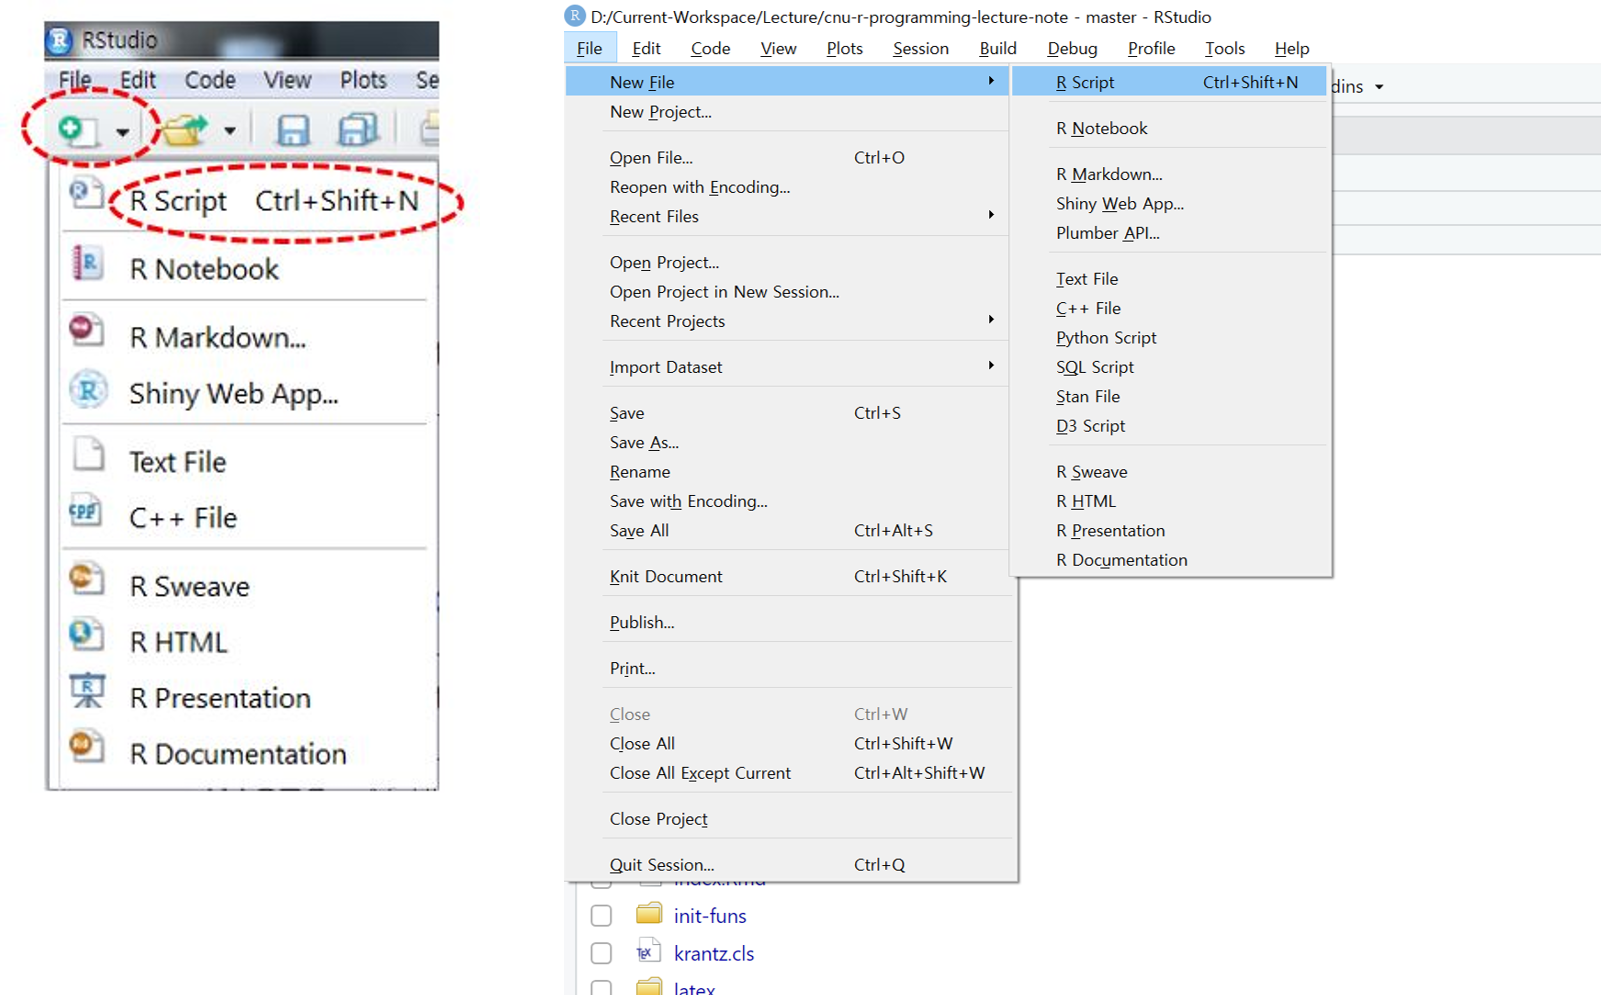
\includegraphics[width=0.8\linewidth]{figures/rstudio-open-new-script} 

}

\caption{RStudio 스크립트 새로 열기}\label{fig:rstudio-new-script}
\end{figure}

\normalsize

\footnotesize

\BeginKnitrBlock{rmdtip}
RStudio는 코딩 및 소스 작성의 효율성을 위해 여러 가지 단축 키를 제공하고 있음. 단축키는 아래 그림과 같이 pull down 메뉴 \texttt{{[}Tools{]}} 또는 \texttt{{[}Help{]}}에서 \texttt{{[}Keyboard\ shortcut\ help{]}} 또는 \texttt{{[}Alt{]}\ +\ {[}Shift{]}\ +\ {[}K{]}} 단축키를 통해 확인할 수 있음. 또는 Rstudio cheatsheet에서 단축키에 대한 정보를 제공하는데 pull down 메뉴 \texttt{{[}Help{]}} \(\rightarrow\) \texttt{{[}Cheatsheets{]}} \(\rightarrow\) \texttt{{[}RStudio\ IDE\ Cheat\ Sheet{]}}을 선택하면 각 아이콘 및 메뉴 기능에 대한 개괄적 설명 확인 가능함.
\EndKnitrBlock{rmdtip}

\normalsize

\textbf{3. 환경/명령기록(Environment/History)} (Figure \ref{fig:rstudio-env})

\begin{itemize}
\tightlist
\item
  \textbf{Environment}: 현재 R 작업환경에 저장되어 있는 객체의 특성 및 값 등을 요약 제시

  \begin{itemize}
  \tightlist
  \item
    좌측 아래 화살표 버튼 클릭: 해당 객체의 상세 정보 확인
  \item
    우측 사각형 버튼 또는 객체(데이터셋명) 클릭: 객체가 데이터셋(데이터프레임)인 경우 스프레드 시트 형태로 데이터셋 확인
  \end{itemize}
\end{itemize}

\footnotesize

\begin{figure}

{\centering 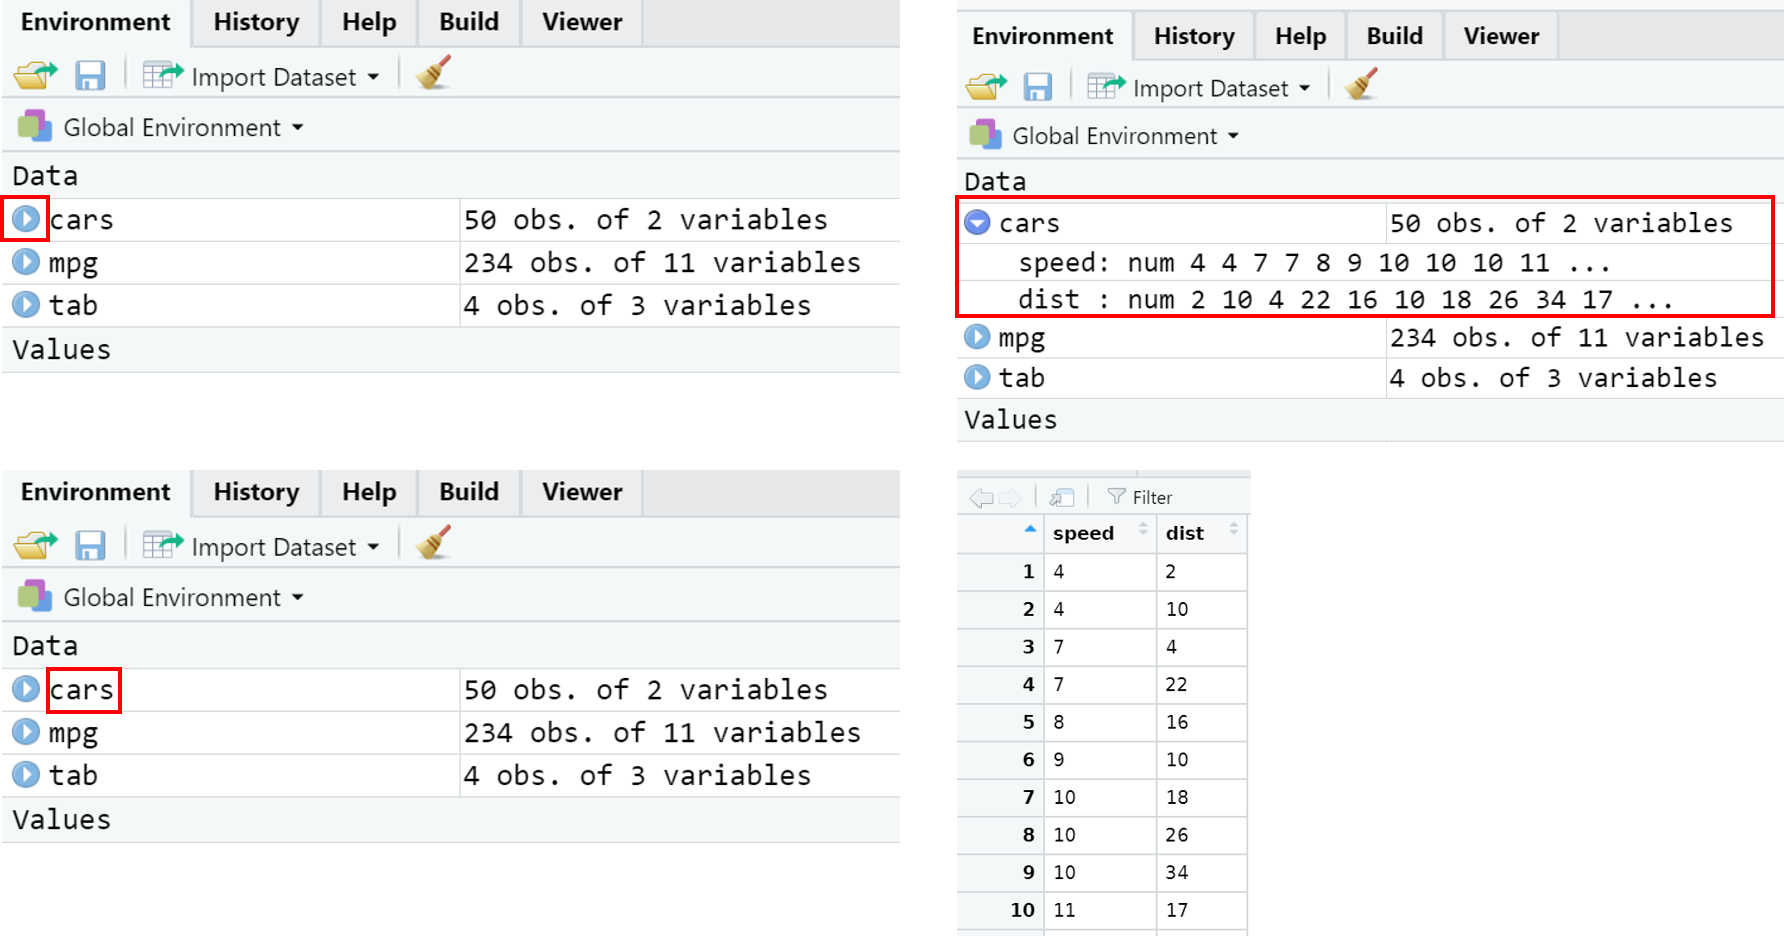
\includegraphics[width=0.9\linewidth]{figures/rstudio-environment} 

}

\caption{RStudio Environment 창 객체 상세 정보 및 스프레드 시트 출력 결과}\label{fig:rstudio-env}
\end{figure}

\normalsize

\begin{itemize}
\tightlist
\item
  History: R 콘솔에서 실행된 명령어(스크립트)들의 이력 확인
\end{itemize}

\footnotesize

\begin{center}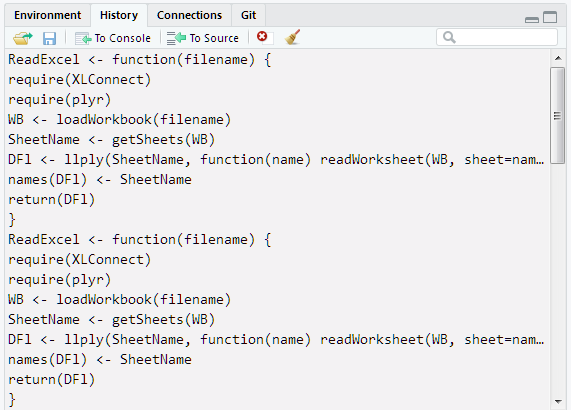
\includegraphics[width=0.9\linewidth]{figures/Rstudio-historywin} \end{center}

\normalsize

\textbf{4. File/Plots/Packages/Help/Viewer}

\begin{itemize}
\tightlist
\item
  File: Windows 파일 탐색기와 유사한 기능 제공

  \begin{itemize}
  \tightlist
  \item
    파일 및 폴더 생성, 삭제/파일 및 폴더명 수정, 그리고 작업경로 설정
  \end{itemize}
\end{itemize}

\footnotesize

\begin{center}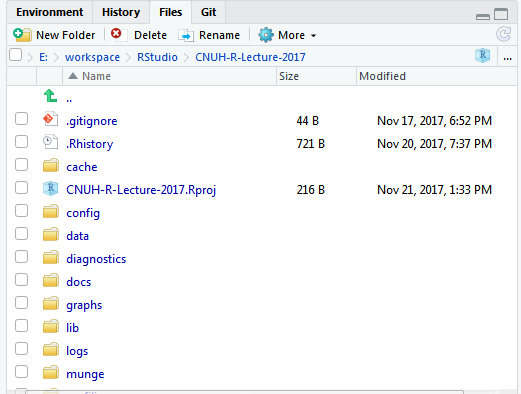
\includegraphics[width=0.8\linewidth]{figures/Rstudio-file} \end{center}

\normalsize

\begin{itemize}
\tightlist
\item
  \textbf{Plots}: 생성한 그래프 출력

  \begin{itemize}
  \tightlist
  \item
    작업 중 생성한 그래프 이력이 Plots 창에 저장: \(\leftarrow\) 이전, \(\rightarrow\) 최근
  \item
    \textbf{\texttt{Zoom}}: 클릭 시 해당 그래프의 팝업창이 생성되고 팝업창의 크기 조정을 통해 그래프의 축소/확대 가능
  \item
    \textbf{\texttt{Export}}: 선택한 그래프를 이미지 파일(\texttt{.png}, \texttt{.jpeg}, \texttt{.pdf} 등)로 저장할 수 있고, 클립보드로 복사 가능
  \end{itemize}
\end{itemize}

\footnotesize

\begin{center}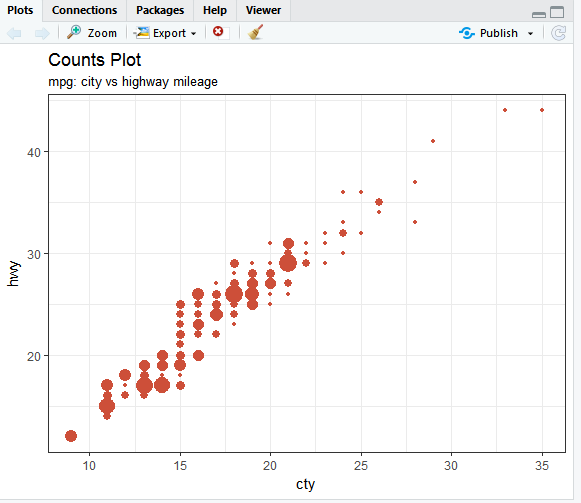
\includegraphics[width=0.8\linewidth]{figures/RStudio-plotwin} \end{center}

\normalsize

\begin{itemize}
\tightlist
\item
  \textbf{Packages}: 현재 컴퓨터에 설치된 R 패키지 목록 출력

  \begin{itemize}
  \tightlist
  \item
    신규 설치 및 업데이트 가능
  \end{itemize}
\end{itemize}

\footnotesize

\begin{center}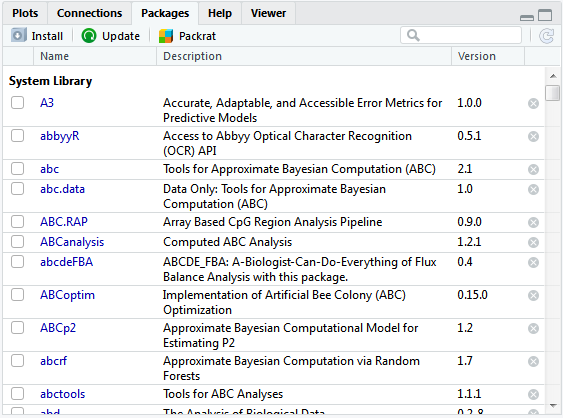
\includegraphics[width=0.8\linewidth]{figures/RStudio-packagewin} \end{center}

\normalsize

\begin{itemize}
\tightlist
\item
  \textbf{Help}: \texttt{help(topic)} 입력 시 도움말 창이 출력되는 공간
\end{itemize}

\footnotesize

\begin{Shaded}
\begin{Highlighting}[]
\KeywordTok{help}\NormalTok{(lm)}
\end{Highlighting}
\end{Shaded}

\normalsize

\footnotesize

\begin{center}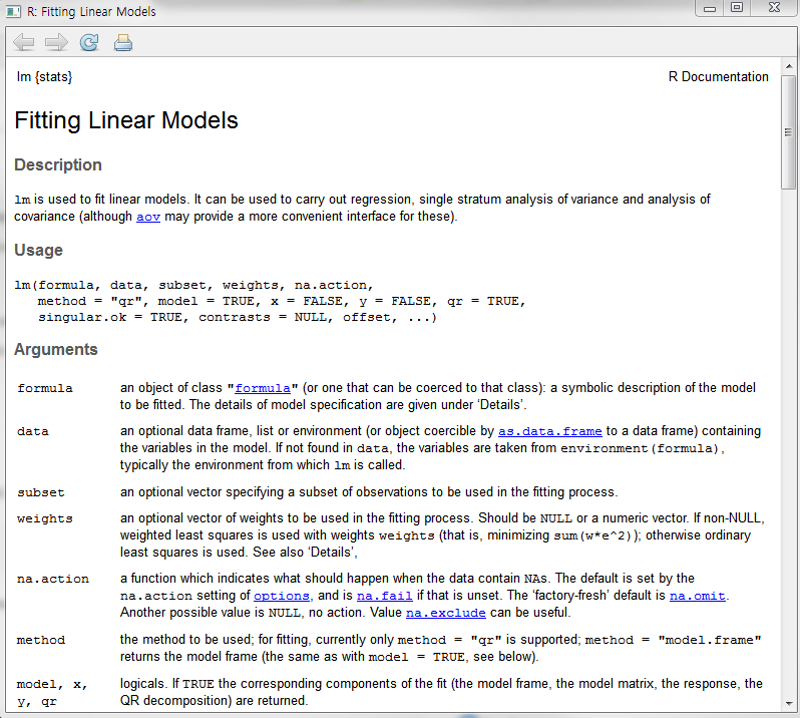
\includegraphics[width=0.8\linewidth]{figures/RStudio-helpwin} \end{center}

\normalsize

\hypertarget{rstudio-glob-options}{%
\subsection{RStudio 환경 설정}\label{rstudio-glob-options}}

Pull-down 메뉴에서 \texttt{{[}Tools{]}} \(\rightarrow\) \texttt{{[}Global\ Options...{]}}를 선택

\footnotesize

\begin{center}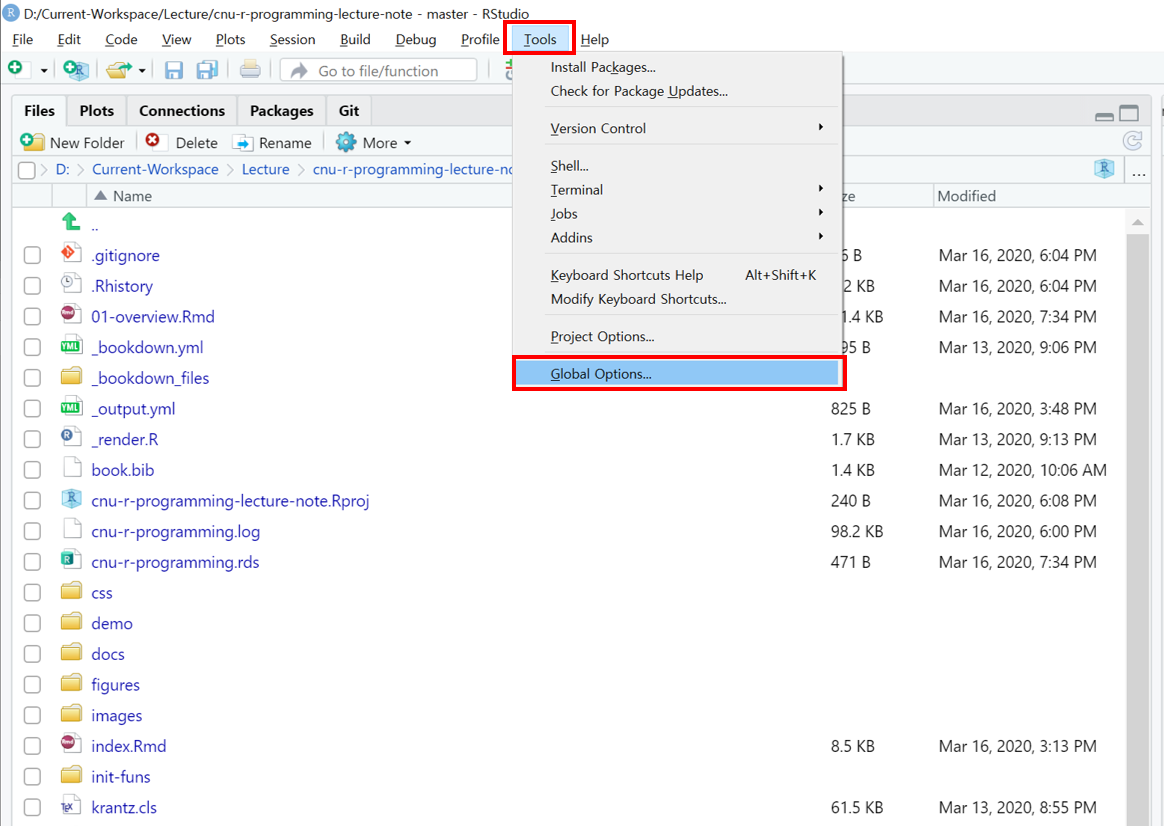
\includegraphics[width=0.8\linewidth]{figures/rstudio-glob-menu} \end{center}

\normalsize

\textbf{General}: RStudio 운용 관련 전반적 설정 세팅

\footnotesize

\begin{figure}

{\centering 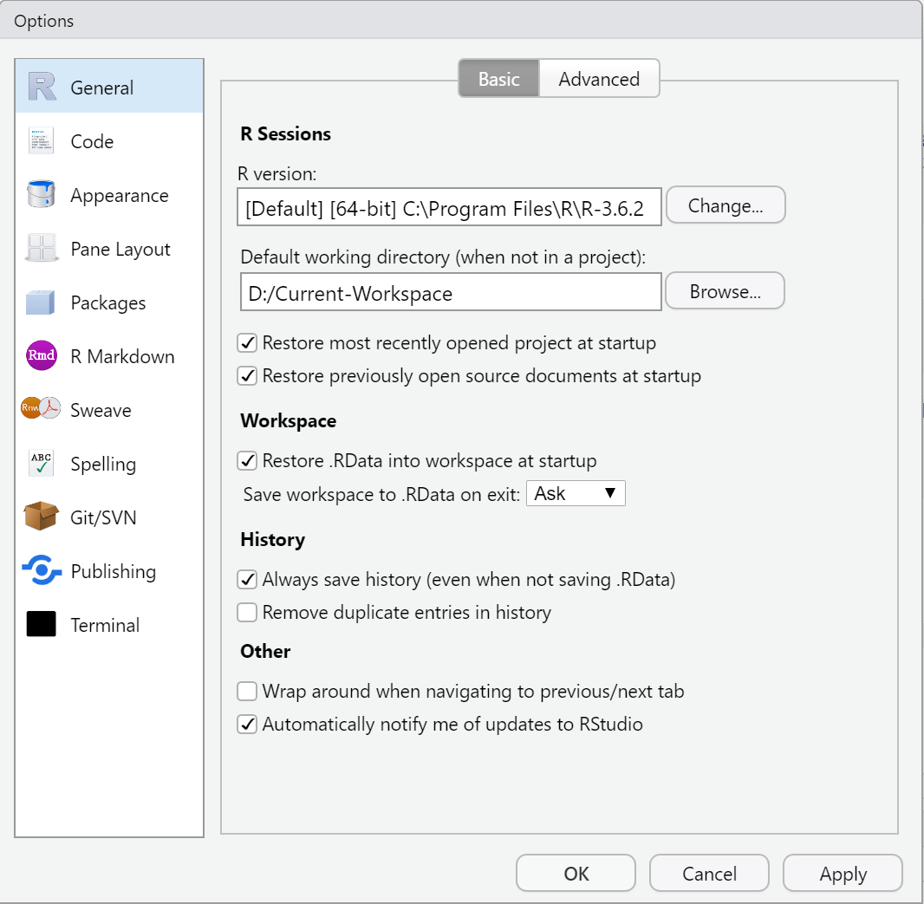
\includegraphics[width=0.8\linewidth]{figures/rstudio-glob-option} 

}

\caption{R General option 팝업 창}\label{fig:rstudio-glob-option}
\end{figure}

\normalsize

\begin{itemize}
\tightlist
\item
  \textbf{R version}: 만약 컴퓨터에 두 개 이상 다른 R 버전이 설치되어 있는 경우 \texttt{{[}Change{]}} 클릭 후 설정 변경 가능
\item
  \textbf{Default Working directory}: 작업 디렉토리 지정({[}\texttt{Browse}{]} 클릭 후 임의 폴더 설정 가능)
\item
  \textbf{Restore most recently opened project at startup}: RStudio 실행 시 가장 최근에 작업한 프로젝트로 이동
\item
  \textbf{Restore previously open source documents at startup}: RStudio 실행 시 현재 프로젝트에서 가장 최근에 작업한 소스코드 문서를 함께 열어줌.
\item
  \textbf{Restore .RData into workspace at startup}: 작업 디렉토리에 존재하는 \texttt{.RData} 파일을 RStudio 실행 시 불러옴
\item
  \textbf{Save workspace to .RData on exit}: R workspace 자동 저장(\texttt{.RData}) 여부
\item
  \textbf{Always save history (even when not saving .RData) }: R 실행 명령 history 저장 여부(Always/Never/Ask)
\item
  \textbf{Remove duplicate entries in history}: history 저장 시 중복 명령 제거 여부
\end{itemize}

작업폴더(Working Directory)는 현재 R session에서 사용하는 기본 폴더로서 R 소스파일 및 데이터의 저장 및 로딩시 기본이 되는 폴더임.

\begin{itemize}
\tightlist
\item
  소스파일이나 데이터를 불러들일 때 작업 폴더에 있는 파일은 경로명을 지정하지 않고 파일명만 사용해도 됨
\item
  작업폴더가 아닌 곳에 있는 파일을 불러들일 때는 경로명까지 써 주어야함.
\item
  R 데이터를 저장할때도 파일명만 쓰면 기본적으로 작업폴더에 저장되며, 다른 폴더에 저장하기 위해서는 경로명까지 써 주어야 함.
\end{itemize}

처음 컴퓨터에 RStudio를 설치하면 Working directory는 Windows 사용자 폴더(예: \texttt{user})의 \texttt{Document} 폴더가 기본값으로 설정되어 있음. 기본 작업폴더를 변경하려면 Figure \ref{fig:rstudio-glob-option}에서 설정 가능.

현재 R session의 작업 디렉토리 설정 방법

\begin{itemize}
\tightlist
\item
  \texttt{{[}Session{]}\ -\textgreater{}\ {[}Set\ Working\ Directoy{]}\ -\textgreater{}\ {[}Choose\ Directory{]}}에서 설정
\end{itemize}

\footnotesize

\begin{center}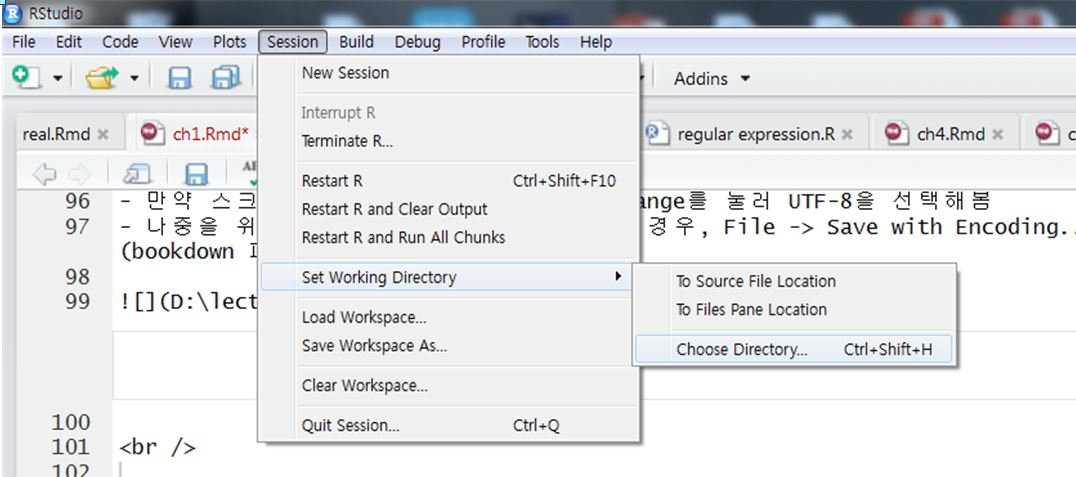
\includegraphics[width=0.8\linewidth]{figures/rstudio-wd-setting} \end{center}

\normalsize

R 콘솔에서 다음과 같은 명령어로 작업폴더를 확인 및 변경 가능

\footnotesize

\begin{Shaded}
\begin{Highlighting}[]
\KeywordTok{getwd}\NormalTok{() }\CommentTok{# 작업폴더 확인}
\end{Highlighting}
\end{Shaded}

\begin{verbatim}
[1] "D:/Current-Workspace/Lecture/cnu-r-programming-lecture-note"
\end{verbatim}

\normalsize

\footnotesize

\begin{Shaded}
\begin{Highlighting}[]
\KeywordTok{setwd}\NormalTok{(}\StringTok{".."}\NormalTok{) }\CommentTok{# 차상위 폴더로 이동}
\KeywordTok{getwd}\NormalTok{()}
\end{Highlighting}
\end{Shaded}

\begin{verbatim}
[1] "D:/Current-Workspace/Lecture"
\end{verbatim}

\begin{Shaded}
\begin{Highlighting}[]
\KeywordTok{setwd}\NormalTok{(}\StringTok{"../.."}\NormalTok{) }\CommentTok{# 차차상위 폴더로 이동}
\KeywordTok{getwd}\NormalTok{()}
\end{Highlighting}
\end{Shaded}

\begin{verbatim}
[1] "D:/"
\end{verbatim}

\begin{Shaded}
\begin{Highlighting}[]
\KeywordTok{setwd}\NormalTok{(}\StringTok{"D:/Current-Workspace/Lecture/misc/"}\NormalTok{) }\CommentTok{# 절대 폴더 명 입력}
\KeywordTok{setwd}\NormalTok{(}\StringTok{".."}\NormalTok{)}
\CommentTok{# dir() # 폴더 내 파일 명 출력}
\KeywordTok{getwd}\NormalTok{()}
\end{Highlighting}
\end{Shaded}

\begin{verbatim}
[1] "D:/Current-Workspace/Lecture"
\end{verbatim}

\begin{Shaded}
\begin{Highlighting}[]
\KeywordTok{setwd}\NormalTok{(}\StringTok{"misc"}\NormalTok{) }\CommentTok{# Current-Workspace 하위폴더인 misc 으로 이동}
\KeywordTok{getwd}\NormalTok{()}
\end{Highlighting}
\end{Shaded}

\begin{verbatim}
[1] "D:/Current-Workspace/Lecture/misc"
\end{verbatim}

\begin{Shaded}
\begin{Highlighting}[]
\KeywordTok{setwd}\NormalTok{(}\StringTok{"D:/Current-Workspace/Lecture/cnu-r-programming-lecture-note/"}\NormalTok{)}
\KeywordTok{getwd}\NormalTok{()}
\end{Highlighting}
\end{Shaded}

\begin{verbatim}
[1] "D:/Current-Workspace/Lecture/cnu-r-programming-lecture-note"
\end{verbatim}

\normalsize

\footnotesize

\BeginKnitrBlock{rmdcaution}
R에서 디렉토리 또는 폴더 구분자는 \texttt{/} 임. Windows에서 사용하는 구분자는 \texttt{\textbackslash{}}인데, R에서 \texttt{\textbackslash{}}는 특수문자로 간주하기 때문에 Windows 의 폴더명을 그대로 사용 시 에러 메세지를 출력함. 이를 해결하기 위해 Windows 경로명을 그대로 복사한 경우 경로 구분자 \texttt{\textbackslash{}} 대신 \texttt{\textbackslash{}\textbackslash{}}로 변경

\textbf{실습}: \texttt{C:\textbackslash{}r-project}를 컴퓨터에 생성 후 해당 폴더를 default 작업폴더로 설정
\EndKnitrBlock{rmdcaution}

\normalsize

\textbf{Code: Editing}: 들여쓰기, 자동 줄바꿈 등 코드 편집에 대한 전반적 설정

\footnotesize

\begin{center}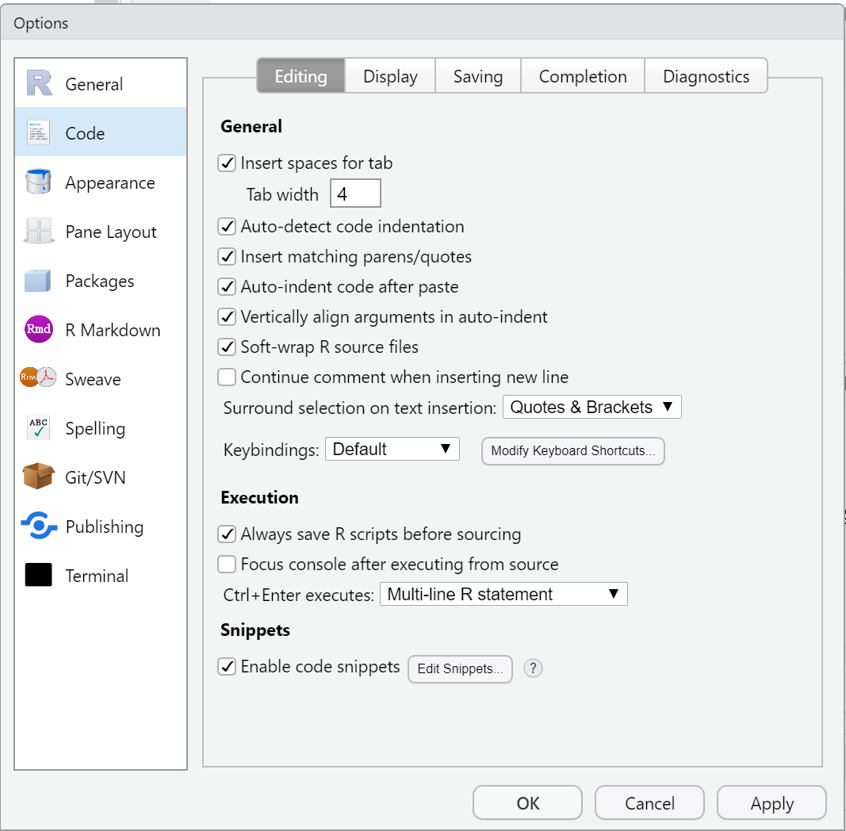
\includegraphics[width=0.8\linewidth]{figures/rstudio-code-edit-option} \end{center}

\normalsize

\begin{itemize}
\tightlist
\item
  \textbf{Insert spaces for tab}: \texttt{{[}Tab{]}} 키를 눌렀을 때 공백(space) 개수 결정(본 강의노트: \texttt{Tab\ width\ =\ 4})
\item
  \textbf{Auto-detect code indentation}: 코들 들여쓰기 자동 감지
\item
  \textbf{Insert matching parens/quotes}: 따옴표, 괄호 입력 시 커서를 따옴표/괄호 사이로 자동 이동
\item
  \textbf{Auto-indent code after paste}: 코드 복사 시 들여쓰기 일괄 적용
\item
  \textbf{Vertically align arguments in auto-indent}: 함수 작성 시 들여쓰기 레벨 유지 여부
\item
  \textbf{Soft-wrap R source file}: 스크립트 편집기 너비를 초과하는 경우 R 코드 행을 자동 줄바꿈
\item
  \textbf{Continue comment when inserting new line}: 주석 표시를 다음 행에도 자동 적용 여부
\item
  \textbf{Surround selection on text insertino}: 스크립트 상 text 선택 후 자동 따옴표 및 괄호 적용 여부
\item
  \textbf{Focus console after executing from source}: 스크립트 실행 후 커서 위치를 콘솔로 이동 여부
\end{itemize}

\textbf{Code: Display}: 스크립트(소스) 에디터 표시 화면 설정

\footnotesize

\begin{center}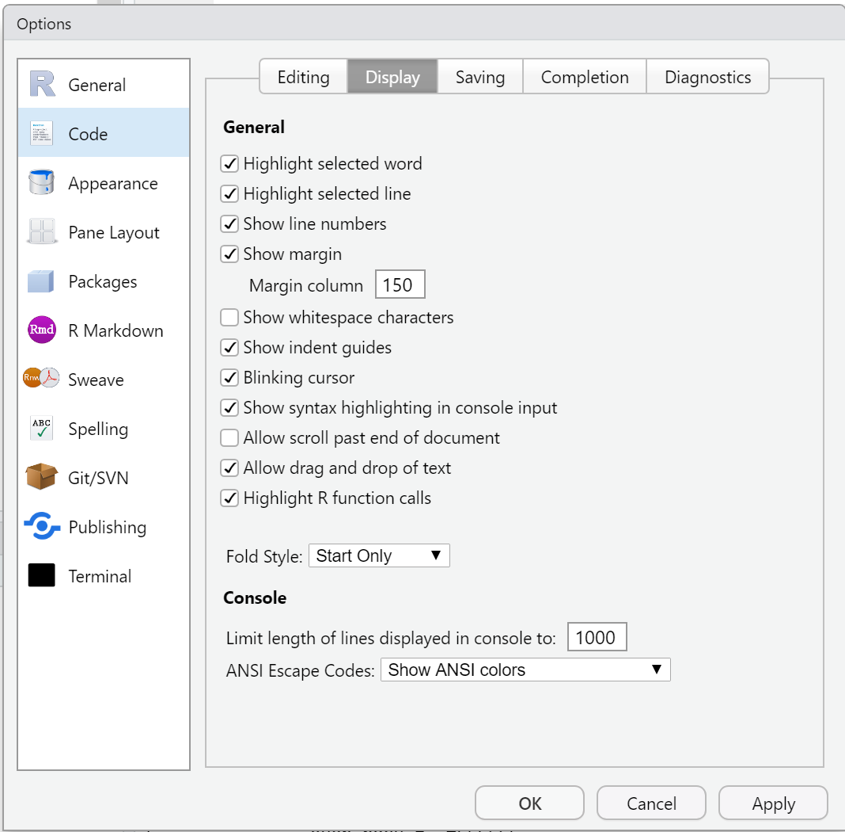
\includegraphics[width=0.8\linewidth]{figures/rstudio-code-display} \end{center}

\normalsize

\begin{itemize}
\tightlist
\item
  \textbf{Highlight selected word}: 스크립트 내 text 선택 시 동일한 text에 대해 배경강조 효과 여부
\item
  \textbf{Highlight selected line}: 선택된 행에 대해 배경 강조효과 여부
\item
  \textbf{Show line numbers}: 행 번호 보여주기 여부
\item
  \textbf{Show margin}: 소스 에디터 오른 쪽에 지정한 margin column 보여주기 여부
\item
  \textbf{Show whitespace characters}: 에디터에 공백 표시 여부
\item
  \textbf{Show indent guides}: 현재 들여쓰기 열 표시 여부
\item
  \textbf{Blinking cursor}: 커서 깜박임 여부
\item
  \textbf{Show syntax highlighting in console output}: 콘솔 입력 라인에 R 구문 강조 표시 적용 여부
\item
  \textbf{Allow scroll past end of document}: 문서 마지막 행 이후 스크롤 허용 여부
\item
  \textbf{Allow drag and drop of text}: 선택한 복수의 행으로 구성된 text에 대해 마우스 drag 허용
\item
  \textbf{Highlight R function calls}: R 내장 및 패키지 제공함수에 대해 강조 여부
\end{itemize}

\textbf{Code: Saving}: 스크립트(소스) 에디터 저장 설정

\footnotesize

\begin{center}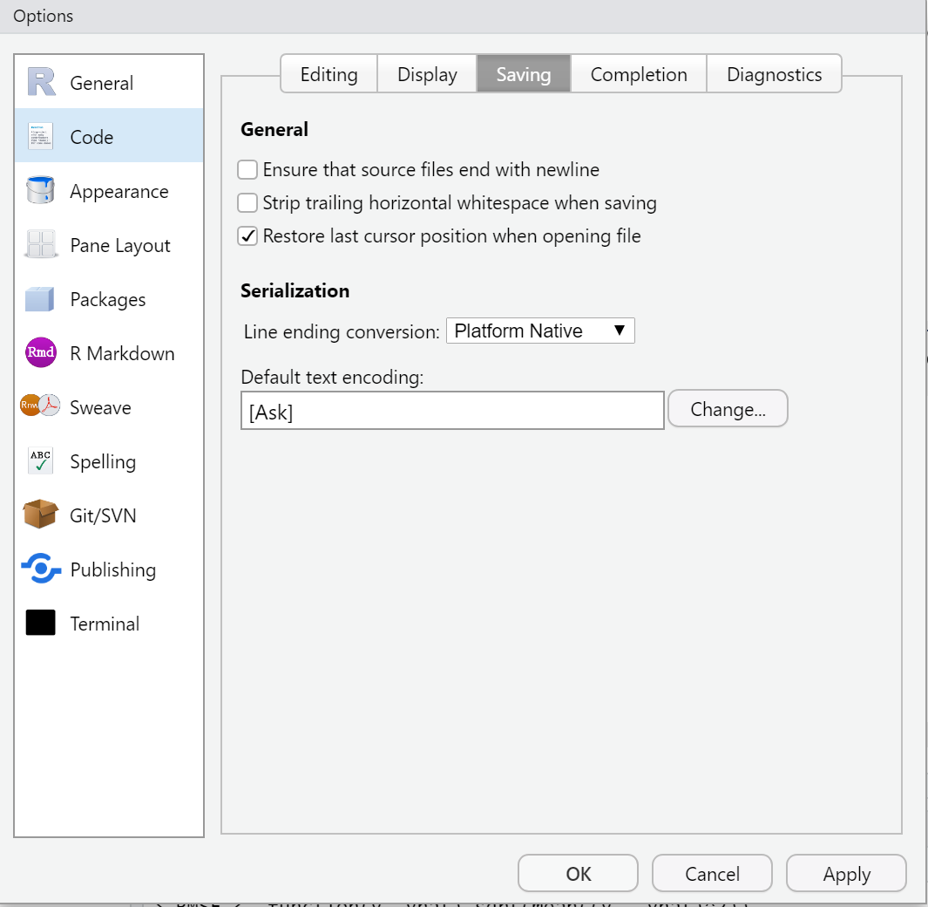
\includegraphics[width=0.8\linewidth]{figures/rstudio-code-saving} \end{center}

\normalsize

\begin{itemize}
\tightlist
\item
  \textbf{Ensure that source file end with newline}
\item
  \textbf{String trailing horizontal whitespace when saving}
\item
  \textbf{Restore last cursor position when opening file}
\item
  \textbf{Default text encoding}: 소스 에디터의 기본 설정 인코딩 설정 변경

  \begin{itemize}
  \tightlist
  \item
    RStudio의 Windows 버전 기본 text encoding은 \texttt{CP949} 임
  \item
    Linux나 Mac OS의 경우 한글은 \texttt{UTF-8}로 인코딩이 설정되어 있음.
  \item
    R 언어는 Linux 환경에서 개발되었기 때문에 \texttt{UTF-8} 인코딩과 호환성이 더 좋음
  \item
    스크립트 파일의 한글이 깨질 때는 \texttt{{[}File{]}\ -\textgreater{}\ {[}Reopen\ with\ Encoding...{]}}에서 encoding 방식 변경
  \end{itemize}
\end{itemize}

\textbf{Appearance}: RStudio 전체 폰트, 폰트 크기, theme 설정

\footnotesize

\begin{center}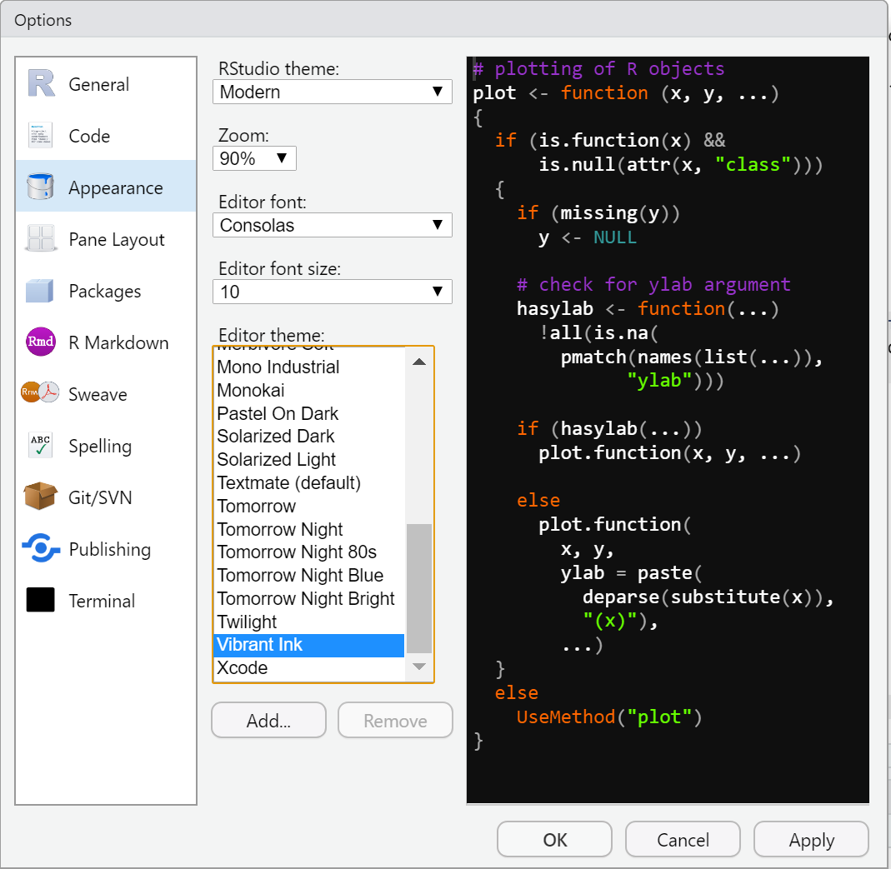
\includegraphics[width=0.8\linewidth]{figures/rstudio-appearance} \end{center}

\normalsize

\begin{itemize}
\tightlist
\item
  본인의 취향에 맞게 폰트 및 테마(theme) 설정
\item
  취향 \(\rightarrow\) 가독성이 제일 좋고 편안한 theme
\end{itemize}

\textbf{Pane Layout}: RStudio 구성 패널들의 위치 및 항목 등을 수정/추가/삭제(4개 페널은 항시 유지)

\footnotesize

\begin{center}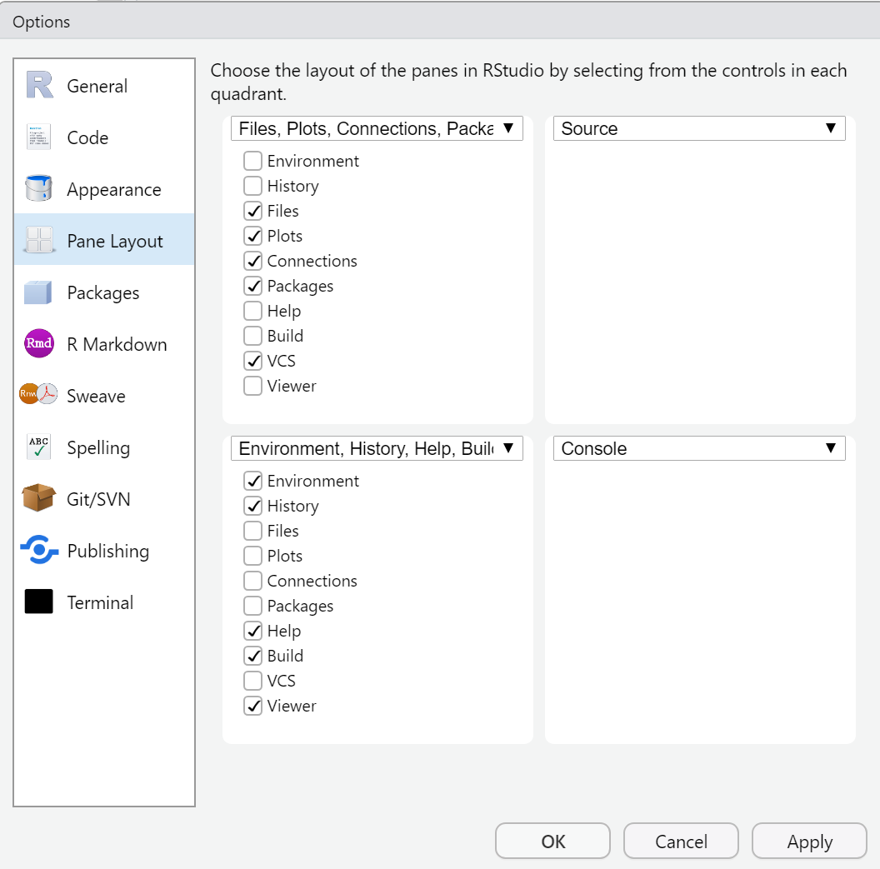
\includegraphics[width=0.8\linewidth]{figures/rstudio-pane-layout} \end{center}

\normalsize

\footnotesize

\BeginKnitrBlock{rmdimportant}
\textbf{실습}: 개인 취향에 맞게 RStudio 에디터 및 theme을 변경해 보자!!
\EndKnitrBlock{rmdimportant}

\normalsize

\hypertarget{rstudio-project}{%
\subsection{RStudio 프로젝트}\label{rstudio-project}}

\begin{enumerate}
\def\labelenumi{\arabic{enumi}.}
\tightlist
\item
  프로젝트

  \begin{itemize}
  \tightlist
  \item
    물리적 측면: 최종 산출물(문서)를 생성하기 위한 데이터, 사진, 그림 등을 모아 놓은 폴더
  \item
    논리적 측면: R session 및 작업의 버전 관리
  \end{itemize}
\item
  프로젝트의 필요성

  \begin{itemize}
  \tightlist
  \item
    자료의 정합성 보장
  \item
    다양한 확장자를 갖는 파일들이 한 폴더 내에 뒤섞일 때 곤란해 질 수 있음
  \item
    실제 분석 및 그래프 생성에 사용한 정확한 프로그램 또는 코드 연결이 어려움
  \end{itemize}
\item
  좋은 프로젝트 구성을 위한 방법

  \begin{itemize}
  \tightlist
  \item
    원자료(raw data)의 보호: 가급적 자료를 읽기 전용(read only) 형태로 다루기
  \item
    데이터 정제(data wrangling 또는 data munging)를 위한 스크립트와 정제 자료를 보관하는 읽기 전용 데이터 디렉토리 생성
  \item
    작성한 스크립트로 생성한 모든 산출물(테이블, 그래프 등)을 ``일회용품''처럼 처리 \(\rightarrow\) 스크립트로 재현 가능
  \item
    한 프로젝트 내 각기 다른 분석마다 다른 하위 디렉토리에 출력결과 저장하는 것이 유용
  \end{itemize}
\item
  RStudio 새로운 프로젝트 생성

  \begin{itemize}
  \tightlist
  \item
    RStudio의 강력하고 유용한 기능
  \item
    새로운 프로젝트 생성: RStudio 메뉴에서 \texttt{{[}File{]}} \(\rightarrow\) \texttt{{[}New\ Project{]}} 선택하면 아래와 같은 팝업 메뉴 생성
  \end{itemize}
\end{enumerate}

\footnotesize

\begin{center}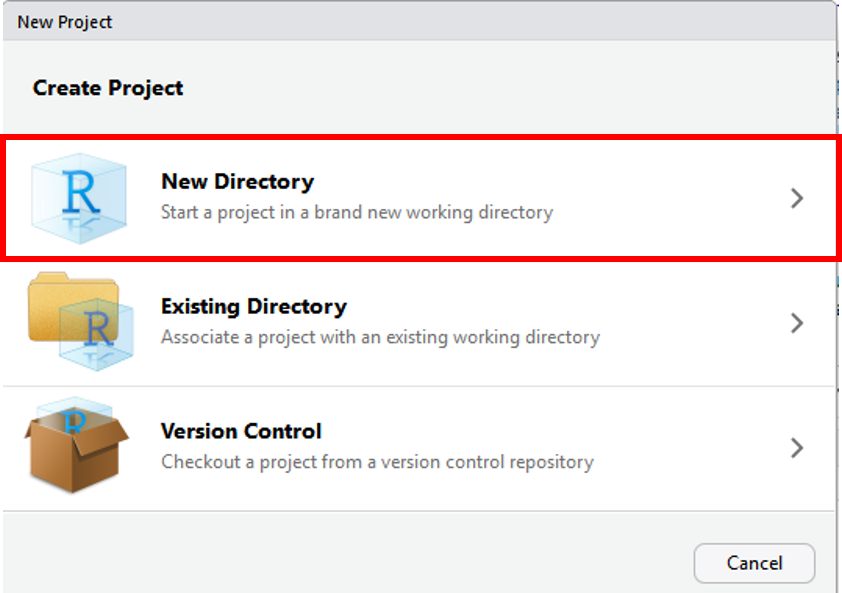
\includegraphics[width=0.8\linewidth]{figures/R-newproject-01} \end{center}

\normalsize

\begin{enumerate}
\def\labelenumi{\arabic{enumi}.}
\setcounter{enumi}{3}
\tightlist
\item
  위 그림에서 \texttt{New\ Directory}를 선택하면 아래와 같은 팝업 창이 나타나면 아래와 같은 프로젝트 유형이 나타남. 여기서는 \texttt{New\ Project} 선택
\end{enumerate}

\footnotesize

\begin{center}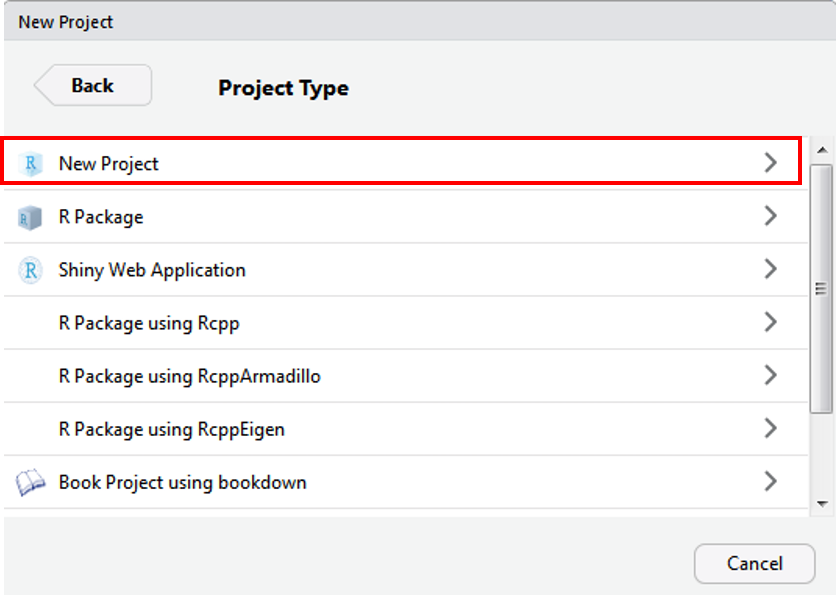
\includegraphics[width=0.8\linewidth]{figures/R-newproject-02} \end{center}

\normalsize

\begin{enumerate}
\def\labelenumi{\arabic{enumi}.}
\setcounter{enumi}{4}
\tightlist
\item
  다음 팝업창에서 새로운 프로젝트의 폴더명을 지정 후 \texttt{Create\ Project} 클릭

  \begin{itemize}
  \tightlist
  \item
    아래 \texttt{{[}Create\ projects\ as\ subdirectories\ of{]}}에서 생성하고자 하는 프로젝트의 상위 디렉토리 설정 \(\rightarrow\) 보통 RStudio의 기본 작업폴더로 설정
  \end{itemize}
\end{enumerate}

\footnotesize

\begin{center}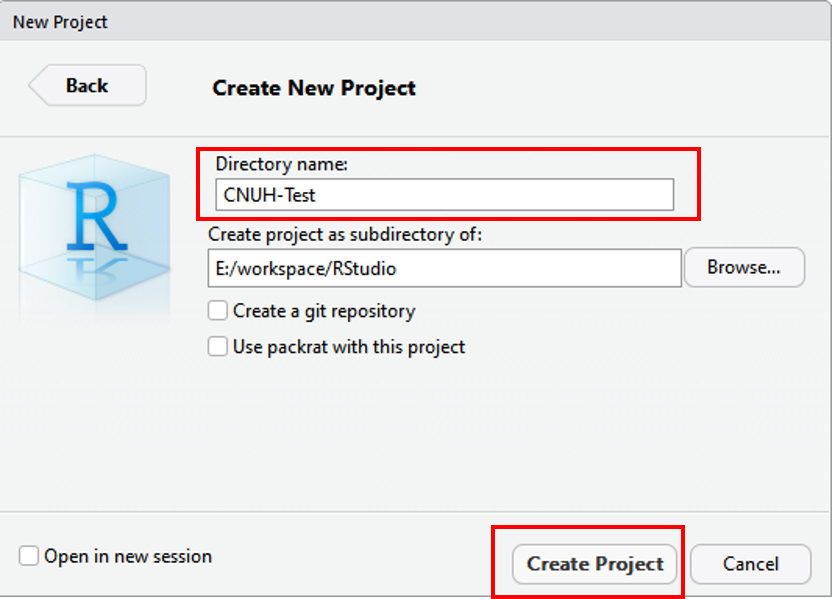
\includegraphics[width=0.8\linewidth]{figures/R-newproject-03} \end{center}

\normalsize

\begin{enumerate}
\def\labelenumi{\arabic{enumi}.}
\setcounter{enumi}{5}
\tightlist
\item
  현재 R session 종료 후 새로운 프로젝트로 session 화면이 열리면 프로젝트 생성 완료
\end{enumerate}

\footnotesize

\BeginKnitrBlock{rmdimportant}
\textbf{실습}: 프로젝트 생성

\begin{itemize}
\tightlist
\item
  위에서 설정한 작업폴더 내에 \texttt{학번-r-programming} 프로젝트 생성
\item
  생성한 프로젝트 폴더 내에 \texttt{docs}, \texttt{figures}, \texttt{script} 폴더 생성
\end{itemize}
\EndKnitrBlock{rmdimportant}

\normalsize

\hypertarget{r-package}{%
\section{R 패키지}\label{r-package}}

\footnotesize

\BeginKnitrBlock{rmdnote}
\textbf{R 패키지(package)}: 특수 목적을 위한 로직으로 구성된 코드들의 집합으로 R에서 구동되는 분석툴을 통칭

\begin{itemize}
\tightlist
\item
  CRAN을 통해 배포: 3자가 이용하기 쉬움 \(\rightarrow\) R 시스템 환경에서 패키지는 가장 중요한 역할
\item
  CRAN \href{https://cran.r-project.org/web/packages/available_packages_by_date.html}{available package by name} 또는 \href{https://cran.r-project.org/web/packages/available_packages_by_name.html}{available package by date}에서 현재 등재된 패키지 리스트 확인 가능
\item
  R console에서 \texttt{available.packages()} 함수를 통해서도 확인 가능
\item
  현재 CRAN 기준(2020-03-17) 배포된 패키지의 개수는 16045 개임
\end{itemize}

\textbf{목적}: RStudio 환경에서 패키지를 설치하고 불러오기
\EndKnitrBlock{rmdnote}

\normalsize

\hypertarget{r-package-path}{%
\subsection{R 패키지 경로 확인 및 변경}\label{r-package-path}}

\begin{itemize}
\tightlist
\item
  패키지 설치 시 일반적으로 R 환경에서 기본값으로 지정한 라이브러리 폴더에 저장
\item
  패키지 설치 전 R 패키지 설치 경로(path) 지정
\item
  \texttt{.libPaths()} 함수를 통해 현재 설정된 패키지 저장 경로 확인
\end{itemize}

\footnotesize

\begin{Shaded}
\begin{Highlighting}[]
\KeywordTok{.libPaths}\NormalTok{()}
\end{Highlighting}
\end{Shaded}

\begin{verbatim}
[1] "C:/Users/user/Documents/R/win-library/3.6"
[2] "C:/Program Files/R/R-3.6.3/library"       
\end{verbatim}

\normalsize

\begin{itemize}
\tightlist
\item
  일반적으로 첫 번째 경로를 디폴트 라이브러리 폴더로 사용
\item
  사용자 지정 라이브러리 경로를 설정 하려면 아래와 같은 절차로 진행
\end{itemize}

\begin{quote}
\textbf{실습: c:/r-library 폴더를 패키지 경로로 지정}
\end{quote}

\begin{enumerate}
\def\labelenumi{\arabic{enumi})}
\item
  \texttt{C:\textbackslash{}}에서 {[}새로 만들기(W){]} -\textgreater{} {[}폴더(F){]} 선택 후 생성 폴더 이름을 \texttt{r-library}로 변경
\item
  윈도우즈 \texttt{{[}제어판{]}\ -\textgreater{}\ {[}시스템\ 및\ 보안{]}\ -\textgreater{}\ {[}시스템{]}\ -\textgreater{}\ {[}고급\ 시스템\ 설정{]}} 클릭
\end{enumerate}

\footnotesize

\begin{center}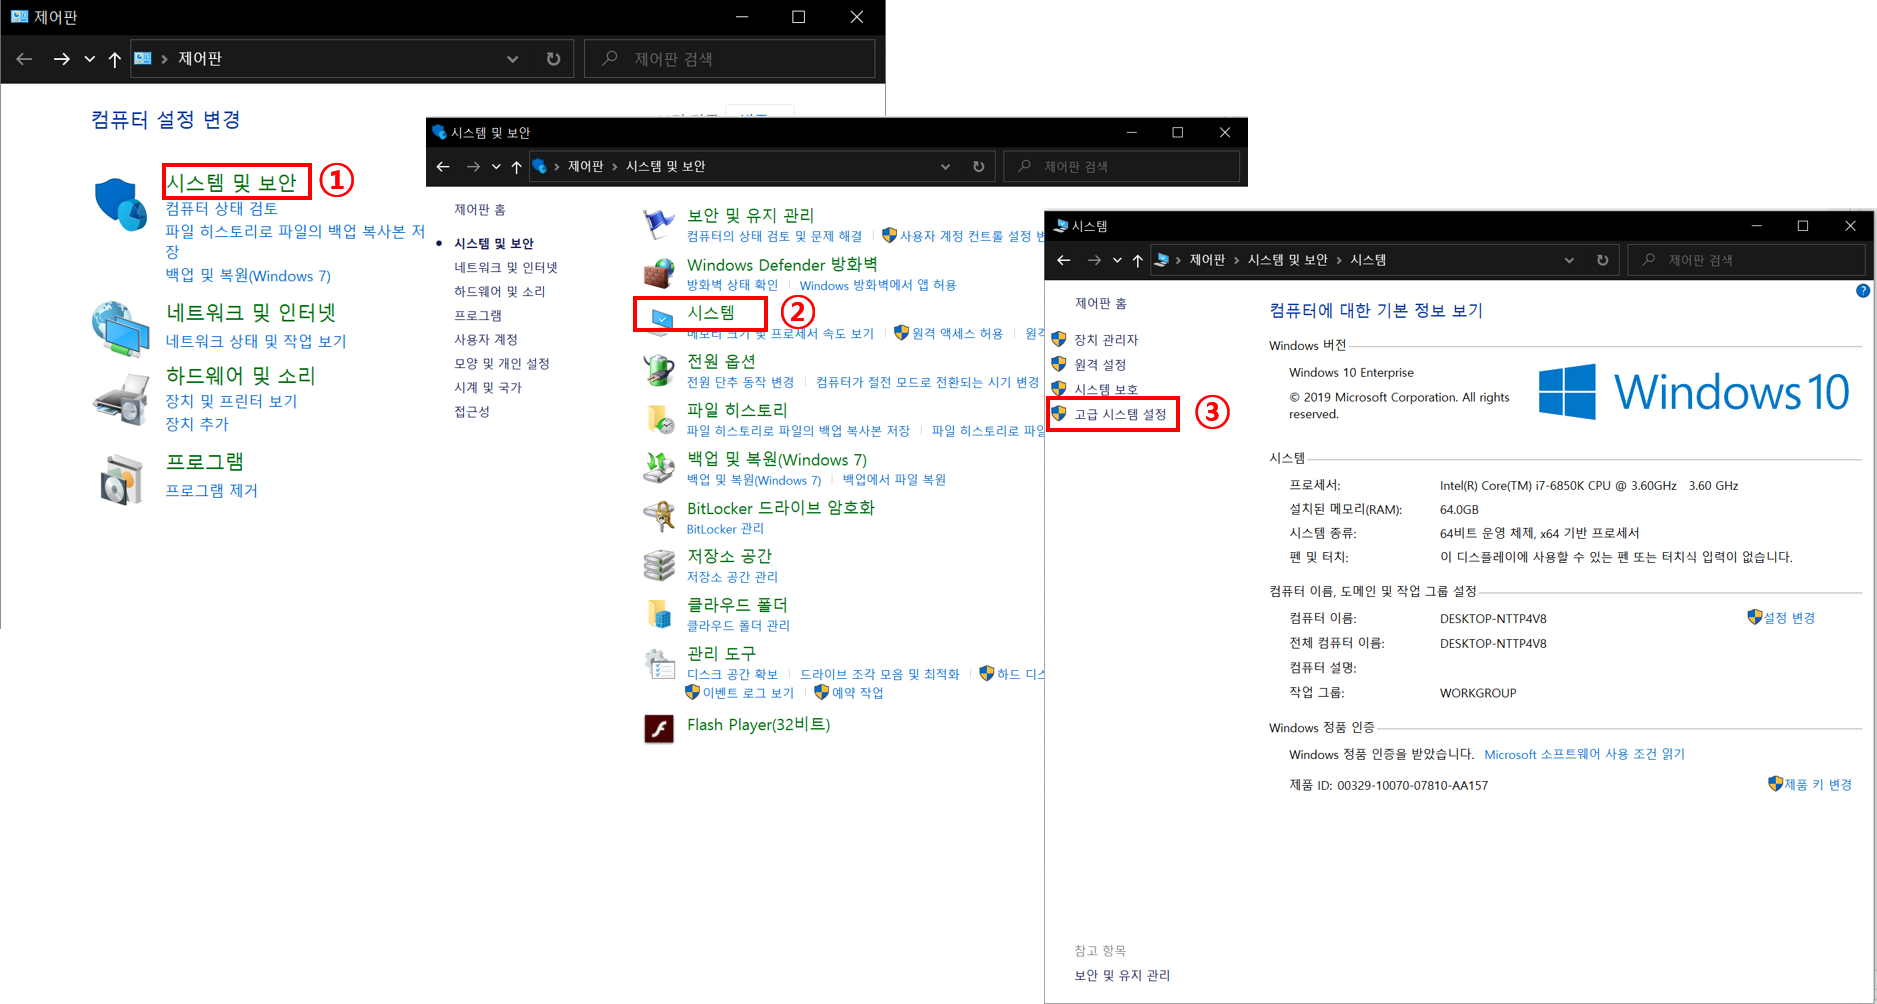
\includegraphics[width=0.8\linewidth]{figures/window-env-system} \end{center}

\normalsize

\begin{enumerate}
\def\labelenumi{\arabic{enumi})}
\setcounter{enumi}{2}
\tightlist
\item
  \texttt{{[}환경변수(N)...{]}} 선택 후 시스템 변수에서 \texttt{{[}새로\ 만들기(W)...{]}} 클릭
\end{enumerate}

\footnotesize

\begin{center}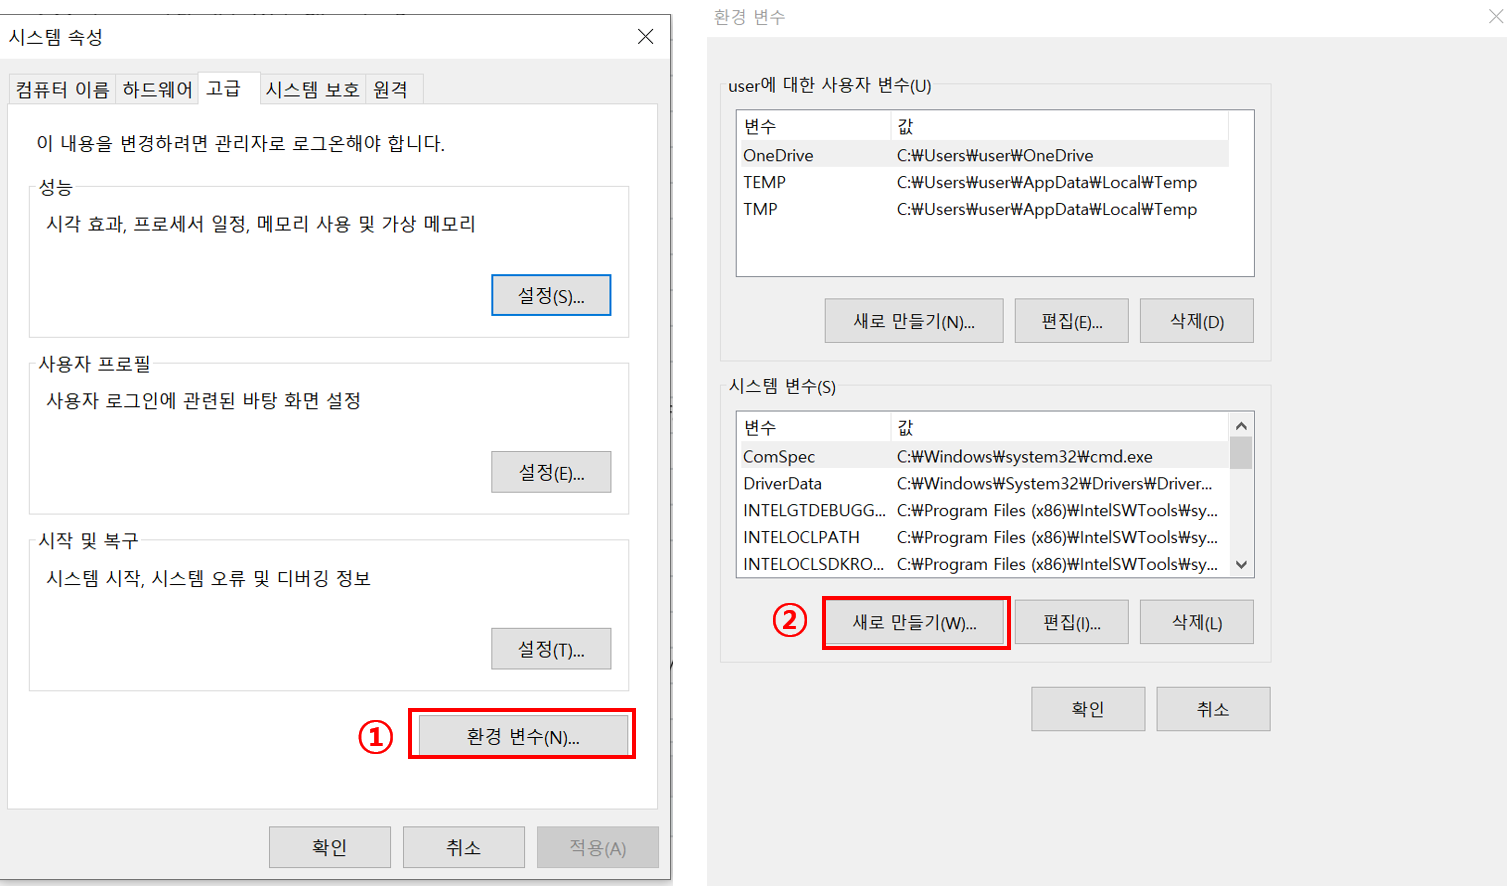
\includegraphics[width=0.8\linewidth]{figures/window-env-var} \end{center}

\normalsize

\begin{enumerate}
\def\labelenumi{\arabic{enumi})}
\setcounter{enumi}{3}
\tightlist
\item
  아래 그림과 같이 변수 이름(N)에 \texttt{R\_LIBS}, 변수 값(V)에 해당 디렉토리 경로 \texttt{C:\textbackslash{}r-library} 입력 후 확인 버튼 클릭
\end{enumerate}

\footnotesize

\begin{center}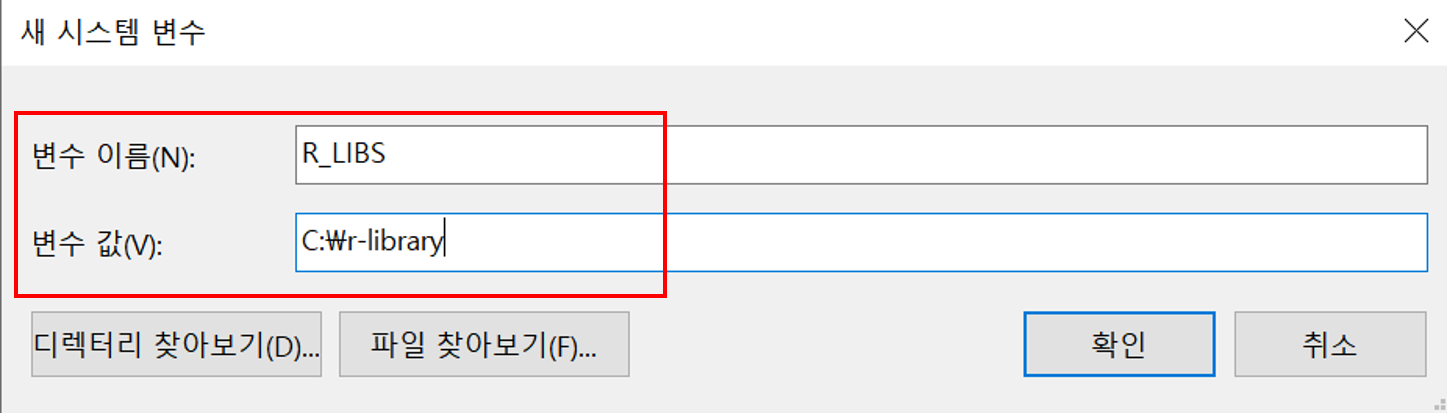
\includegraphics[width=0.9\linewidth]{figures/window-new-system-var} \end{center}

\normalsize

\begin{enumerate}
\def\labelenumi{\arabic{enumi})}
\setcounter{enumi}{4}
\tightlist
\item
  현재 RStudio 종료 후 재실행한 다음 콘솔창에 \texttt{.libPaths()} 입력 후 라이브러리 경로 확인
\end{enumerate}

\hypertarget{r-package-install}{%
\subsection{R 패키지 설치하기}\label{r-package-install}}

\begin{itemize}
\tightlist
\item
  RStudio 메뉴 \texttt{{[}Tools{]}} \(\rightarrow\) \texttt{{[}Install\ packages{]}} 클릭 후 생성된 팝업 창에서 설치하고자 하는 패키지 입력 후 설치
\end{itemize}

\footnotesize

\begin{center}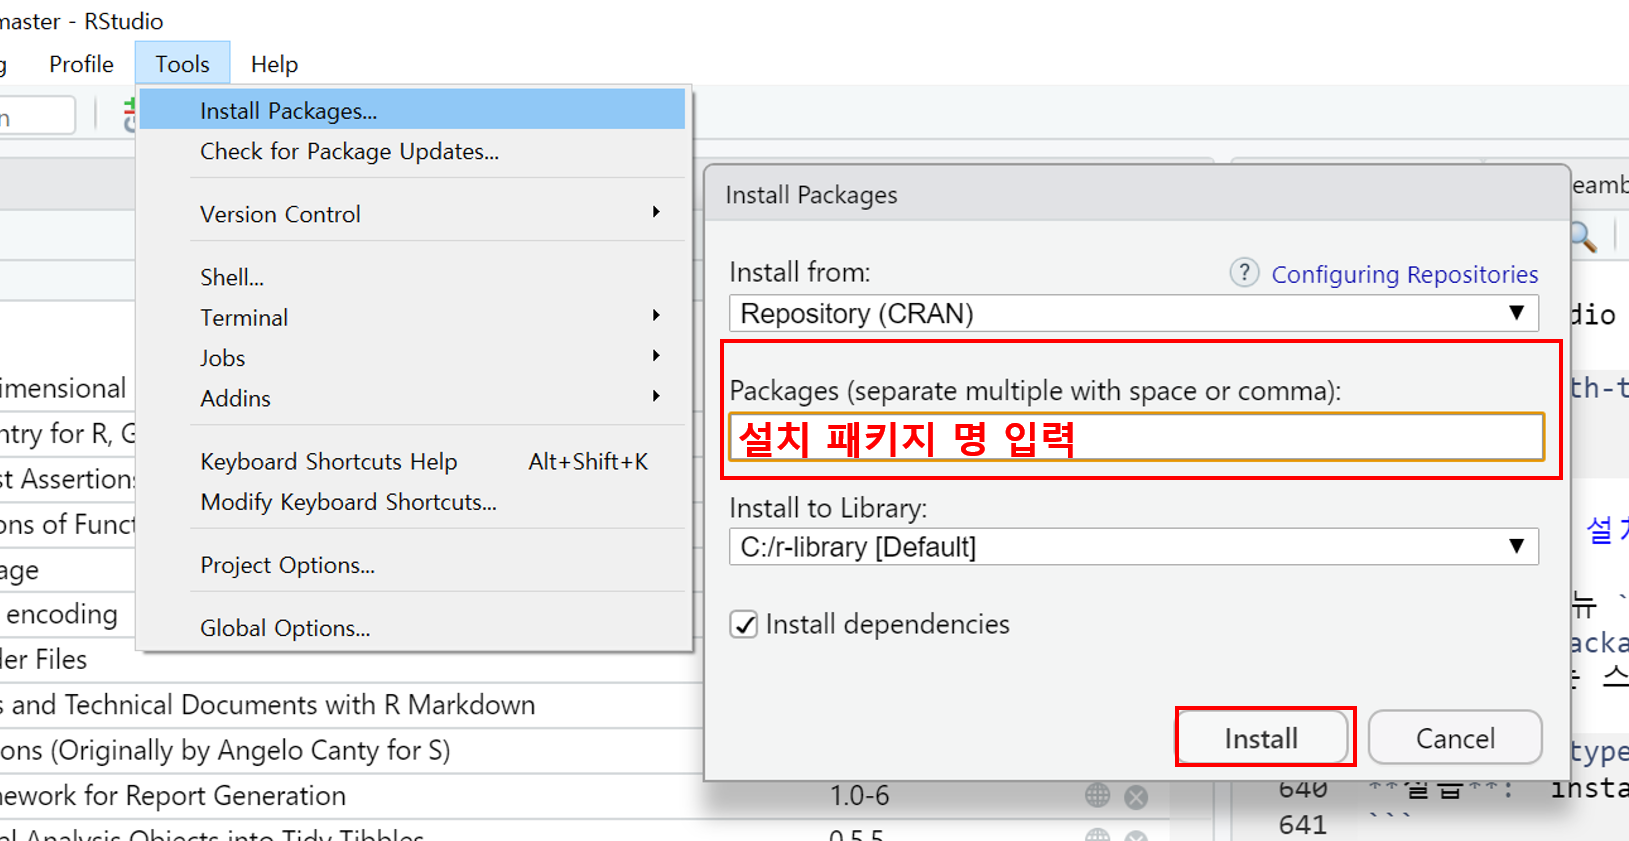
\includegraphics[width=0.8\linewidth]{figures/rstudio-package-install} \end{center}

\normalsize

\begin{itemize}
\tightlist
\item
  RStudio \texttt{Packages} 창에서 \texttt{{[}Install{]}} 버튼 누르면 위와 동일한 팝업창이 나타남(위와 동일)
\end{itemize}

\footnotesize

\begin{center}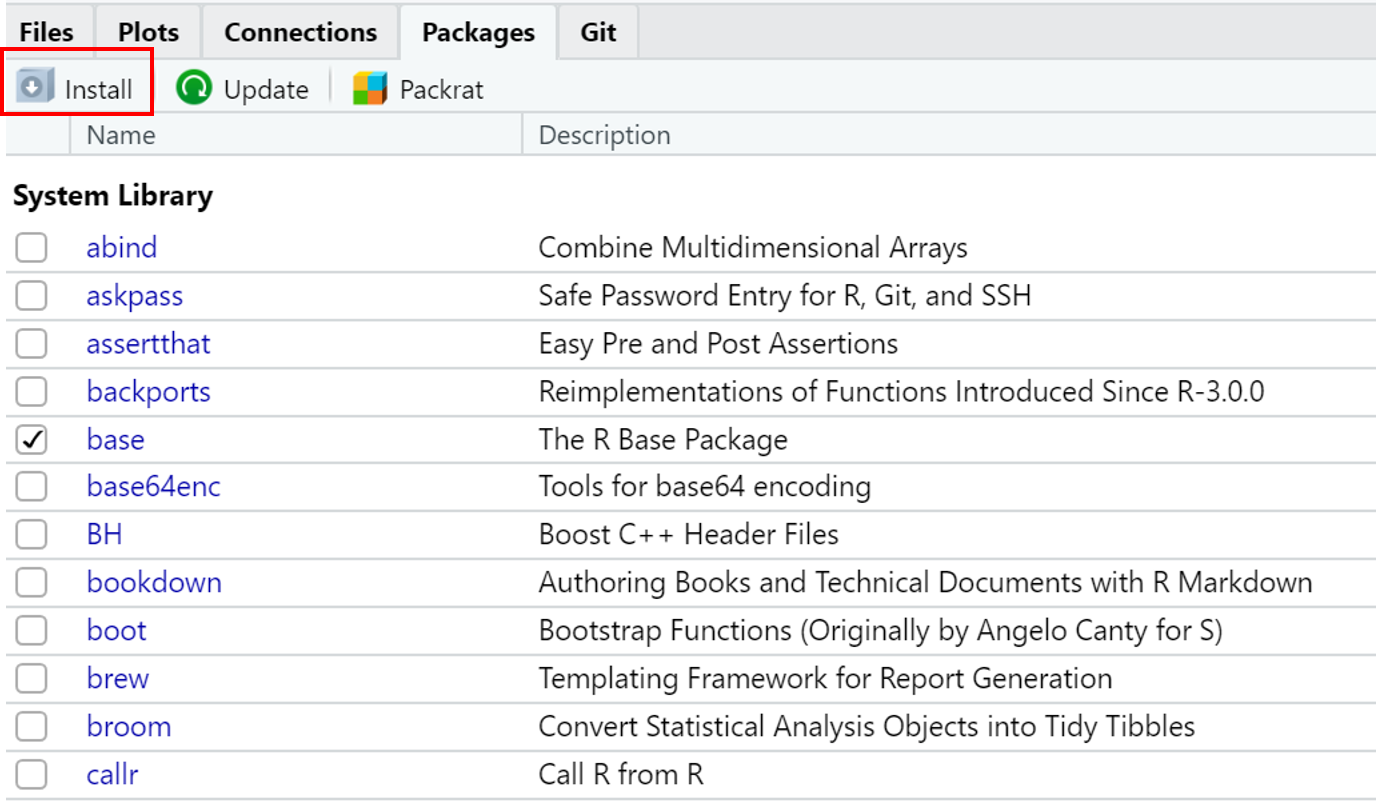
\includegraphics[width=0.8\linewidth]{figures/rstudio-pack-win-02} \end{center}

\normalsize

\begin{itemize}
\tightlist
\item
  R 콘솔 또는 스크립트 창에서 \texttt{install.packages(package\_name)} 함수를 사용해서 패키지 설치
\end{itemize}

\footnotesize

\BeginKnitrBlock{rmdimportant}
\textbf{실습}: \texttt{install.packages()} 함수를 이용해 \texttt{tidyverse} 패키지 설치
\EndKnitrBlock{rmdimportant}

\normalsize

\footnotesize

\begin{Shaded}
\begin{Highlighting}[]
\KeywordTok{install.packages}\NormalTok{(}\StringTok{"tidyverse"}\NormalTok{)}
\end{Highlighting}
\end{Shaded}

\normalsize

\begin{quote}
위 명령어를 실행하면 \texttt{tidyverse} 패키지 뿐 아니라 연관된 패키지들이 동시에 설치됨
\end{quote}

\hypertarget{r-package-load}{%
\subsection{R 패키지 불러오기}\label{r-package-load}}

\begin{enumerate}
\def\labelenumi{\arabic{enumi}.}
\tightlist
\item
  \texttt{library()} vs.~\texttt{require()}

  \begin{itemize}
  \tightlist
  \item
    \texttt{library()}: 불러오고자 하는 패키지가 시스템에 존재하지 않는 경우 에러 메세지 출력(에러 이후 명령어들이 실행되지 않음)
  \item
    \texttt{require()}: 패키지가 시스템에 존재하지 않는 경우 경고 메세지 출력(경고 이후 명령어 정상적으로 실행)
  \end{itemize}
\item
  다중 패키지 동시에 불러오기

  \begin{itemize}
  \tightlist
  \item
    RStudio \texttt{Packages} 창에서 설치하고자 하는 패키지 선택 버튼 클릭하면 R workspace로 해당 패키지 로드 가능
  \item
    스크립트 이용
  \end{itemize}
\end{enumerate}

\footnotesize

\BeginKnitrBlock{rmdimportant}
\textbf{실습}: \texttt{tidyverse} 패키지 불러오기
\EndKnitrBlock{rmdimportant}

\normalsize

\footnotesize

\begin{Shaded}
\begin{Highlighting}[]
\KeywordTok{require}\NormalTok{(tidyverse)}
\end{Highlighting}
\end{Shaded}

\begin{verbatim}
필요한 패키지를 로딩중입니다: tidyverse
\end{verbatim}

\begin{verbatim}
-- Attaching packages ----------------------------------------------------------------------------------------------------------------------------------- tidyverse 1.3.0 --
\end{verbatim}

\begin{verbatim}
v ggplot2 3.3.0     v purrr   0.3.3
v tibble  2.1.3     v dplyr   0.8.5
v tidyr   1.0.2     v stringr 1.4.0
v readr   1.3.1     v forcats 0.5.0
\end{verbatim}

\begin{verbatim}
-- Conflicts -------------------------------------------------------------------------------------------------------------------------------------- tidyverse_conflicts() --
x dplyr::filter()     masks stats::filter()
x dplyr::group_rows() masks kableExtra::group_rows()
x dplyr::lag()        masks stats::lag()
\end{verbatim}

\normalsize

\footnotesize

\BeginKnitrBlock{rmdnote}
실무에서 R의 활용능력은 패키지 활용 여부에 달려 있음. 즉, 목적에 맞는 업무를 수행하기 위해 가장 적합한 패키지를 찾고 활용하느냐에 따라 R 활용능력의 차이를 보임. 앞서 언급한 바와 같이 CRAN에 등록된 패키지는 16000 개가 넘지만, 이 중 많이 활용되고 있는 패키지의 수는 약 200 \textasciitilde{} 300 개 내외이고, 실제 데이터 분석 시 10 \textasciitilde{} 20개 정도의 패키지가 사용됨. 앞 예제에서 설치하고 불러온 \texttt{tidyverse} 패키지는 Hadley Wickham \citep{tidyverse2019}이 개발한 데이터 전처리 및 시각화 패키지 번들이고, 현재 R 프로그램 환경에 지대한 영향을 미침. 본 강의 ``데이터프레임 가공 및 시각화''에서 해당 패키지 활용 방법을 배울 예정
\EndKnitrBlock{rmdnote}

\normalsize

\hypertarget{r-basic}{%
\section{R 기초 문법}\label{r-basic}}

\footnotesize

\BeginKnitrBlock{rmdnote}
본 절에서 다루는 R 문법은 R 입문 시 객체(object)의 명명 규칙과 R 콘솔 창에서 가장 빈번하게 사용되는 기초적인 명령어만 다룰 예정임. 심화 내용은 2-3주 차에 다룰 예정임.
\EndKnitrBlock{rmdnote}

\normalsize

\begin{itemize}
\tightlist
\item
  R은 객체지향언어(object-oriented language)

  \begin{itemize}
  \tightlist
  \item
    객체(object): 숫자, 데이터셋, 단어, 테이블, 분석결과 등 모든 것을 칭함
  \item
    ``객체지향''의 의미는 R의 모든 명령어는 객체를 대상으로 이루어진다는 것을 의미
  \end{itemize}
\end{itemize}

\footnotesize

\BeginKnitrBlock{rmdtip}
알아두면 유용한(콘솔창에서 매우 많이 사용되는) 명령어 및 단축키

\begin{itemize}
\tightlist
\item
  \texttt{ls()}: 현재 R 작업공간에 저장된 모든 객체 리스트 출력
\item
  \texttt{rm(object\_name)}: \texttt{object\_name}에 해당하는 객체 삭제
\item
  \texttt{rm(list\ =\ ls())}: R 작업공간에 저장된 모든 객체들을 일괄 삭제
\item
  단축키 \texttt{{[}Ctrl{]}\ +\ {[}L{]}}: R 콘솔 창 일괄 청소
\item
  단축키 \texttt{{[}Ctrl{]}\ +\ {[}Shift{]}\ +\ {[}F10{]}}: R session 초기화
\end{itemize}

\textbf{예시}
\EndKnitrBlock{rmdtip}

\normalsize

\footnotesize

\begin{Shaded}
\begin{Highlighting}[]
\NormalTok{x <-}\StringTok{ }\DecValTok{7}
\NormalTok{y <-}\StringTok{ }\DecValTok{1}\OperatorTok{:}\DecValTok{30} \CommentTok{#1에서 30까지 정수 입력}
\KeywordTok{ls}\NormalTok{() }\CommentTok{#현재 작업공간 내 객체명 출력}
\end{Highlighting}
\end{Shaded}

\begin{verbatim}
 [1] "a"                  "b"                  "cars"              
 [4] "def.chunk.hook"     "fig_cap"            "hook_output"       
 [7] "tab"                "x"                  "y"                 
[10] "도움말 보기 명령어" "사용법"             "설명"              
\end{verbatim}

\normalsize

\footnotesize

\begin{Shaded}
\begin{Highlighting}[]
\KeywordTok{rm}\NormalTok{(x) }\CommentTok{# 객체 x 삭제}
\KeywordTok{ls}\NormalTok{()}
\end{Highlighting}
\end{Shaded}

\begin{verbatim}
 [1] "a"                  "b"                  "cars"              
 [4] "def.chunk.hook"     "fig_cap"            "hook_output"       
 [7] "tab"                "y"                  "도움말 보기 명령어"
[10] "사용법"             "설명"              
\end{verbatim}

\begin{Shaded}
\begin{Highlighting}[]
\KeywordTok{rm}\NormalTok{(a,b) }\CommentTok{# 객체 a,b 동시 삭제}
\KeywordTok{ls}\NormalTok{()}
\end{Highlighting}
\end{Shaded}

\begin{verbatim}
[1] "cars"               "def.chunk.hook"     "fig_cap"           
[4] "hook_output"        "tab"                "y"                 
[7] "도움말 보기 명령어" "사용법"             "설명"              
\end{verbatim}

\begin{Shaded}
\begin{Highlighting}[]
\CommentTok{# rm(list = ls()) # 모든 객체 삭제}
\end{Highlighting}
\end{Shaded}

\normalsize

\hypertarget{r-object-nam-rule}{%
\subsubsection*{R 객체 입력 방법 및 변수 설정 규칙}\label{r-object-nam-rule}}


객체를 할당하는 두 가지 방법:\texttt{=}, \texttt{\textless{}-}

\begin{itemize}
\tightlist
\item
  두 할당 지시자의 차이점

  \begin{itemize}
  \tightlist
  \item
    \texttt{=}: 명령의 최상 수준에서만 사용 가능
  \item
    \texttt{\textless{}-}: 어디서든 사용 가능
  \item
    함수 호출과 동시에 변수에 값을 할당할 목적으로는 \texttt{\textless{}-}만 사용 가능
  \end{itemize}
\end{itemize}

\footnotesize

\begin{Shaded}
\begin{Highlighting}[]
\CommentTok{# mean(): 입력 벡터의 평균 계산}
\KeywordTok{mean}\NormalTok{(y <-}\StringTok{ }\DecValTok{1}\OperatorTok{:}\DecValTok{5}\NormalTok{)}
\end{Highlighting}
\end{Shaded}

\begin{verbatim}
[1] 3
\end{verbatim}

\begin{Shaded}
\begin{Highlighting}[]
\NormalTok{y}
\end{Highlighting}
\end{Shaded}

\begin{verbatim}
[1] 1 2 3 4 5
\end{verbatim}

\begin{Shaded}
\begin{Highlighting}[]
\KeywordTok{mean}\NormalTok{(}\DataTypeTok{x =} \DecValTok{1}\OperatorTok{:}\DecValTok{5}\NormalTok{)}
\end{Highlighting}
\end{Shaded}

\begin{verbatim}
[1] 3
\end{verbatim}

\begin{Shaded}
\begin{Highlighting}[]
\NormalTok{x}
\end{Highlighting}
\end{Shaded}

\begin{verbatim}
Error in eval(expr, envir, enclos): 객체 'x'를 찾을 수 없습니다
\end{verbatim}

\normalsize

객체 또는 변수의 명명 규칙

\begin{itemize}
\tightlist
\item
  알파벳, 한글, 숫자, \texttt{\_}, \texttt{.}의 조합으로 구성 가능(\texttt{-}은 사용 불가)
\item
  변수명의 알파벳, 한글, \texttt{.}로 시작 가능
\item
  \texttt{.}로 시작한 경우 뒤에 숫자 올 수 없음(숫자로 인지)
\item
  대소문자 구분
\end{itemize}

\footnotesize

\begin{Shaded}
\begin{Highlighting}[]
\CommentTok{# 1:10은 1부터 10까지 정수 생성}
\CommentTok{# 'c()'는 벡터 생성 함수}
\NormalTok{x <-}\StringTok{ }\KeywordTok{c}\NormalTok{(}\DecValTok{1}\OperatorTok{:}\DecValTok{10}\NormalTok{) }
\CommentTok{# 1:10으로 구성된 행렬 생성}
\NormalTok{X <-}\StringTok{ }\KeywordTok{matrix}\NormalTok{(}\KeywordTok{c}\NormalTok{(}\DecValTok{1}\OperatorTok{:}\DecValTok{10}\NormalTok{), }\DataTypeTok{nrow =} \DecValTok{2}\NormalTok{, }\DataTypeTok{ncol =} \DecValTok{5}\NormalTok{, }\DataTypeTok{byrow =}\NormalTok{ T)}
\NormalTok{x}
\end{Highlighting}
\end{Shaded}

\begin{verbatim}
 [1]  1  2  3  4  5  6  7  8  9 10
\end{verbatim}

\begin{Shaded}
\begin{Highlighting}[]
\NormalTok{X}
\end{Highlighting}
\end{Shaded}

\begin{verbatim}
     [,1] [,2] [,3] [,4] [,5]
[1,]    1    2    3    4    5
[2,]    6    7    8    9   10
\end{verbatim}

\begin{Shaded}
\begin{Highlighting}[]
\CommentTok{# 논리형 객체}
\NormalTok{.x <-}\StringTok{ }\OtherTok{TRUE}
\NormalTok{.x}
\end{Highlighting}
\end{Shaded}

\begin{verbatim}
[1] TRUE
\end{verbatim}

\begin{Shaded}
\begin{Highlighting}[]
\CommentTok{# 알파벳 + 숫자}
\CommentTok{# seq(): 수열을 만드는 함수}
\CommentTok{# 1 에서부터(from) 10 까지(to) 공차가 2(by)인 수열}
\NormalTok{a1 <-}\StringTok{ }\KeywordTok{seq}\NormalTok{(}\DataTypeTok{from =} \DecValTok{1}\NormalTok{, }\DataTypeTok{to =} \DecValTok{10}\NormalTok{, }\DataTypeTok{by =} \DecValTok{2}\NormalTok{)}
\CommentTok{# 한글 변수명}
\NormalTok{가수 <-}\StringTok{ }\KeywordTok{c}\NormalTok{(}\StringTok{"Damian Rice"}\NormalTok{, }\StringTok{"Beatles"}\NormalTok{, }\StringTok{"최백호"}\NormalTok{, }\StringTok{"Queen"}\NormalTok{, }\StringTok{"Carlos Gardel"}\NormalTok{, }\StringTok{"BTS"}\NormalTok{, }\StringTok{"조용필"}\NormalTok{)}
\NormalTok{가수}
\end{Highlighting}
\end{Shaded}

\begin{verbatim}
[1] "Damian Rice" "Beatles" "최백호"
"Queen"
[5] "Carlos Gardel" "BTS" "조용필"
\end{verbatim}

\normalsize

\begin{enumerate}
\def\labelenumi{\arabic{enumi}.}
\setcounter{enumi}{2}
\tightlist
\item
  잘못된 객체 또는 변수 명명 예시
\end{enumerate}

\footnotesize

\begin{Shaded}
\begin{Highlighting}[]
\NormalTok{3x <-}\StringTok{ }\DecValTok{7}
\end{Highlighting}
\end{Shaded}

\begin{verbatim}
Error: <text>:1:2: 예상하지 못한 기호(symbol)입니다.
1: 3x
     ^
\end{verbatim}

\normalsize

\footnotesize

\begin{Shaded}
\begin{Highlighting}[]
\NormalTok{_x <-}\StringTok{ }\KeywordTok{c}\NormalTok{(}\StringTok{"M"}\NormalTok{, }\StringTok{"M"}\NormalTok{, }\StringTok{"F"}\NormalTok{)}
\end{Highlighting}
\end{Shaded}

\begin{verbatim}
Error: <text>:1:1: 예상하지 못한 입력입니다.
1: _
    ^
\end{verbatim}

\normalsize

\footnotesize

\begin{Shaded}
\begin{Highlighting}[]
\FloatTok{.3}\NormalTok{ <-}\StringTok{ }\DecValTok{10}
\end{Highlighting}
\end{Shaded}

\begin{verbatim}
Error in 0.3 <- 10: 대입에 유효하지 않은 (do_set) 좌변입니다
\end{verbatim}

\normalsize

\hypertarget{r-markdown-get-start}{%
\section{R Markdown (맛보기)}\label{r-markdown-get-start}}

\footnotesize

\BeginKnitrBlock{rmdnote}
\protect\hyperlink{r-basic}{R 기초 문법} 절과 마찬가지로 R Markdown을 이용해 최소한의 문서(\texttt{html} 문서)를 작성하고 생성하는 방법에 대해 기술함. R Markdown에 대한 보다 상세한 내용은 본 수업의 마지막 주차에 다룰 예정임.
\EndKnitrBlock{rmdnote}

\normalsize

\begin{enumerate}
\def\labelenumi{\arabic{enumi}.}
\tightlist
\item
  R Markdown은 R 코드와 분석 결과(표, 그림 등)을 포함한 문서 또는 컨텐츠를 제작하는 도구로 일반적으로 아래 열거한 형태로 활용함

  \begin{itemize}
  \tightlist
  \item
    문서 또는 논문(\texttt{pdf}, \texttt{html}, \texttt{docx})
  \item
    프리젠테이션(\texttt{pdf}, \texttt{html}, \texttt{pptx})
  \item
    웹 또는 블로그
  \end{itemize}
\item
  재현가능(reproducible)한 분석 및 연구\footnote{과학적 연구의 결과물을 오픈소스로 내놓고 누구라도 검증 가능} 가능

  \begin{itemize}
  \tightlist
  \item
    신뢰성 있는 문서 작성
  \item
    \texttt{Copy\ \&\ paste}를 하지 않고 효율적 작업 가능
  \end{itemize}
\item
  R Markdown 문서를 통해 최종 결과물(\texttt{pdf}, \texttt{html}, \texttt{docx})이 도출되는 process

  \begin{itemize}
  \tightlist
  \item
    현재 공식적인 프로세스는 \texttt{knitr} + \texttt{rmarkdown} + \texttt{pandoc} + \texttt{RStudio} + \texttt{github}
  \end{itemize}
\end{enumerate}

\footnotesize

\begin{figure}

{\centering 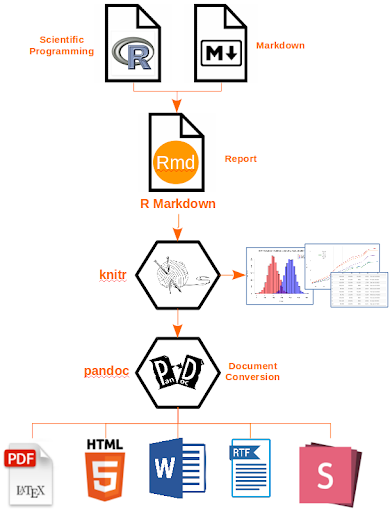
\includegraphics[width=0.6\linewidth]{figures/rmarkdown-flow} 

}

\caption{R Markdown의 최종 결과물 산출과정(http://applied-r.com/project-reporting-template/)}\label{fig:rmarkdown-flow}
\end{figure}

\normalsize

\hypertarget{create-rmd-file}{%
\subsubsection*{R Markdown 문서 시작하기}\label{create-rmd-file}}


\begin{itemize}
\tightlist
\item
  \textbf{R Markdown} 문서 생성: \texttt{{[}File{]}\ -\textgreater{}\ {[}New\ File{]}\ -\textgreater{}\ {[}R\ Markdown..{]}}을 선택
\end{itemize}

\footnotesize

\BeginKnitrBlock{rmdcaution}
RStudio를 처음 설치하고 위와 같이 진행할 경우 아래와 같은 패키지 설치 여부를 묻는 팝업 창이 나타남. 패키지 설치 여부에 \texttt{{[}Yes{]}}를 클릭하면 R Markdown 문서 생성을 위해 필요한 패키지들이 자동으로 설치
\EndKnitrBlock{rmdcaution}

\normalsize

\footnotesize

\begin{center}\includegraphics[width=0.8\linewidth]{figures/rmarkdown-new-01} \end{center}

\normalsize

\begin{itemize}
\tightlist
\item
  설치 완료 후 R Markdown으로 생성할 최종 문서 유형 선택 질의 창이 나타남. 아래 창에서 제목(Title)과 저자(Author) 이름 입력 후 \texttt{{[}OK{]}} 버튼 클릭(\texttt{Document}, \texttt{html} 문서 선택)
\end{itemize}

\footnotesize

\begin{center}\includegraphics[width=0.8\linewidth]{figures/rmarkdown-new-02} \end{center}

\normalsize

\begin{itemize}
\tightlist
\item
  아래 그림과 같이 새로운 문서 창이 생성되고 \texttt{test.Rmd} 파일로 저장\footnote{\protect\hyperlink{rstudio-project}{RStudio 프로젝트}에서 생성한 폴더 내에 파일 저장}
\end{itemize}

\footnotesize

\begin{center}\includegraphics[width=0.8\linewidth]{figures/rmarkdown-new-03} \end{center}

\normalsize

\begin{itemize}
\tightlist
\item
  문서 상단에 \texttt{Knit} 아이콘을 클릭 후 \texttt{Knit\ to\ HTML} 클릭 또는 문서 아무 곳에 커서를 위치하고 단축키 \texttt{{[}Ctrl{]}\ +\ {[}Shift{]}\ +\ {[}K{]}} 입력
\end{itemize}

\footnotesize

\begin{center}\includegraphics[width=0.8\linewidth]{figures/rmarkdown-new-04} \end{center}

\normalsize

\begin{itemize}
\tightlist
\item
  \texttt{knitr} + \texttt{R\ Markdown} + \texttt{pandoc} \(\rightarrow\) \texttt{html} 파일 생성 결과
\end{itemize}

\footnotesize

\begin{figure}

{\centering \includegraphics[width=0.8\linewidth]{figures/rmarkdown-new-out} 

}

\caption{test.html 문서 화면(저장 폴더 내 `test.html`을 크롬 브라우저로 실행)}\label{fig:rmarkdown-new-out}
\end{figure}

\normalsize

\hypertarget{r-markdown-uxbb38uxc11c-uxad6cuxc131}{%
\subsubsection{R Markdown 문서 구성}\label{r-markdown-uxbb38uxc11c-uxad6cuxc131}}

R Markdown 문서는 아래 그림과 같이 \textbf{YAML}, \textbf{Markdown 텍스트}, \textbf{Code Chunk} 세 부분으로 구성됨.

\footnotesize

\begin{center}\includegraphics[width=0.8\linewidth]{figures/rmarkdown-part} \end{center}

\normalsize

\textbf{1. YAML (YAML Ain't Markup Language)}

\begin{itemize}
\tightlist
\item
  R Markdown 문서의 metadata로 문서의 맨 처음에 항상 포함되어야 함.
\item
  R Markdown 문서의 최종 출력 형태, 제목, 저자, 날짜 등의 정보 등을 포함
\item
  YAML 언어에 대한 사용 예시는 \citet{xie-2016} 의 \href{https://bookdown.org/yihui/bookdown/r-markdown.html}{Appendix B.2} 참고
\item
  최소 형태의 YAML 예시
\end{itemize}

\footnotesize

\begin{Shaded}
\begin{Highlighting}[]
\OtherTok{---}
\FunctionTok{title:}\AttributeTok{ }\StringTok{"Hello R Markdown"}
\FunctionTok{author:}\AttributeTok{ }\StringTok{"Zorba"}
\FunctionTok{date:}\AttributeTok{ }\StringTok{"2020-03-17"}
\FunctionTok{output:}\AttributeTok{ html_document}
\OtherTok{---}
\end{Highlighting}
\end{Shaded}

\normalsize

\textbf{2. Markdown 텍스트}

\begin{itemize}
\tightlist
\item
  Markdown 문법은 15주 차 강의에서 배울 예정임
\item
  \href{https://rstudio.com/wp-content/uploads/2015/03/rmarkdown-reference.pdf}{R Markdown 레퍼런스 가이드} 참조
\item
  그림 삽입: \texttt{!{[}{]}(path/filename)}
\end{itemize}

\begin{Shaded}
\begin{Highlighting}[]
\NormalTok{그립 삽입 구문}
\NormalTok{![](figures/son.jpg)   }
\end{Highlighting}
\end{Shaded}

\includegraphics{figures/son.jpg}

\textbf{3. Code Chunk}

\begin{itemize}
\tightlist
\item
  실제 R code가 실행되는 부분임
\item
  Code chunk 실행 시 다양한 옵션들이 있으나 이 부분 역시 15주 차 강의에서 간략히 다룰 예정임
\item
  Code chunk는 \texttt{\textasciigrave{}\textasciigrave{}\textasciigrave{}\{r\}}로 시작되며 \texttt{r}은 code 언어 이름을 나타냄.
\item
  Code chunk는 \texttt{\textasciigrave{}\textasciigrave{}\textasciigrave{}} 로 종료
\item
  R Markdown 문서 작성 시 단축키 \texttt{{[}Ctrl{]}\ +\ {[}Alt{]}\ +\ {[}I{]}}를 입력하면 Chunk 입력창이 자동 생성됨
\item
  Chunk option에 대한 상세 내용은 \url{https://yihui.org/knitr/options/} 또는 \href{https://rstudio.com/wp-content/uploads/2015/03/rmarkdown-reference.pdf}{R Markdown 레퍼런스 가이드} 참조
\end{itemize}

\begin{Shaded}
\begin{Highlighting}[]
\NormalTok{Code chunk 예시}

\NormalTok{Xie의 R Markdown: The Definitive Guide에서 발췌}

\BaseNTok{```\{r\}}
\BaseNTok{fit = lm(dist ~ speed, data = cars)}
\BaseNTok{b   = coef(fit)}
\BaseNTok{plot(cars)}
\BaseNTok{abline(fit)}
\BaseNTok{```}
\end{Highlighting}
\end{Shaded}

\footnotesize

\begin{Shaded}
\begin{Highlighting}[]
\NormalTok{fit =}\StringTok{ }\KeywordTok{lm}\NormalTok{(dist }\OperatorTok{~}\StringTok{ }\NormalTok{speed, }\DataTypeTok{data =}\NormalTok{ cars)}
\NormalTok{b   =}\StringTok{ }\KeywordTok{coef}\NormalTok{(fit)}
\KeywordTok{plot}\NormalTok{(cars)}
\KeywordTok{abline}\NormalTok{(fit)}
\end{Highlighting}
\end{Shaded}

\includegraphics{01-overview_files/figure-latex/unnamed-chunk-44-1.pdf}

\normalsize

\begin{itemize}
\tightlist
\item
  Code chunk에서 외부 그림 파일 불러오기(\citet{xie-2018} 에서 예시 발췌)
\end{itemize}

\footnotesize

\begin{Shaded}
\begin{Highlighting}[]
\NormalTok{knitr}\OperatorTok{::}\KeywordTok{include_graphics}\NormalTok{(}\KeywordTok{rep}\NormalTok{(}\StringTok{'figures/knit-logo.png'}\NormalTok{, }\DecValTok{3}\NormalTok{))}
\end{Highlighting}
\end{Shaded}

\includegraphics[width=0.328\linewidth]{figures/knit-logo} \includegraphics[width=0.328\linewidth]{figures/knit-logo} \includegraphics[width=0.328\linewidth]{figures/knit-logo}

\normalsize

\footnotesize

\BeginKnitrBlock{rmdimportant}
\textbf{Homework 1}: R Markdown 문서에 아래 내용을 포함한 문서를 \texttt{html} 파일 형식으로 출력 후 제출

\begin{itemize}
\tightlist
\item
  간략한 자기소개 및 ``통계 프로그래밍 언어'' 수업에 대한 본인만의 목표 기술
\item
  본인이 setting 한 RStudio 구성 캡쳐 화면을 그림 파일로 저장하고 R Markdown 문서에 삽입(화면 캡쳐 시 생성 프로젝트 내 폴더 내용 반드시 포함)
\item
  패키지 \texttt{ggplot2}를 불러오고 \texttt{cars} 데이터셋의 2차원 산점도(\textbf{hint}: \texttt{help(geom\_point)} 또는 googling 활용)를 문서에 포함
\end{itemize}
\EndKnitrBlock{rmdimportant}

\normalsize

\hypertarget{data-type}{%
\chapter{R 객체(R object)}\label{data-type}}

\footnotesize

\BeginKnitrBlock{rmdnote}
\textbf{학습목표(2 주차)}: R에서 사용 가능한 데이터 타입에 대해 알아보고, 고유 데이터 타입으로 구성한 객체(스칼라, 백터, 리스트)와 이와 연관된 함수들을 익힌다.
\EndKnitrBlock{rmdnote}

\normalsize

\hypertarget{ch2-abstract}{%
\subsubsection*{학습 필요성}\label{ch2-abstract}}


\begin{itemize}
\tightlist
\item
  R언어는 타 프로그래밍 언어와 유사한 데이터 타입(정수형, 실수형, 문자형 등)을 제공
\item
  R 언어가 다른 언어와 차이점 \(\rightarrow\) \textbf{데이터 분석}에 특화된 벡터(vector), 행렬(matrix), 데이터프레임(data frame), 리스트(list)와 같은 객체\footnote{R에서 사용자가 데이터 입력을 위해 생성 또는 읽어온 객체(object)는 종종 변수(variable)라는 말과 혼용. 본 문서에서는 최상위 데이터 저장장소를 객체라고 명명하며 데이터프레임과 같이 여러 종류의 데이터타입으로 이루어진 객체의 1차원 속성을 변수라고 칭함} 제공
\item
  R 패키지에서 제공되는 함수 사용 방법은 R의 객체에 따라 달라질 수 있음\\
\item
  R 언어를 원활히 다룰 수 있으려면 R에서 데이터 객체의 형태, 자료 할당 및 그 연산 방법에 대한 이해가 필수적으로 선행되어야 함
\end{itemize}

\hypertarget{object-value}{%
\subsubsection*{R의 데이터 타입}\label{object-value}}


\begin{itemize}
\item
  \textbf{수치형(numeric)}: 숫자(정수, 소수)
\item
  \textbf{문자열(string)}: \texttt{"충남대학교"}, \texttt{"R강의"}
\item
  \textbf{논리형(logical)}: \texttt{TRUE}/\texttt{FALSE}
\item
  \textbf{결측값(\texttt{NA})}: 자료에서 발생한 결측 표현
\item
  \textbf{공백(\texttt{NULL})}: 지정하지 않은 값
\item
  \textbf{요인(factor)}: 범주형 자료 표현(수치 + 문자 결합 형태로 이해하면 편함)
\item
  \textbf{기타}: 숫자아님(\texttt{NaN}), 무한대(\texttt{Inf}) 등
\end{itemize}

\hypertarget{ch2-object-type}{%
\subsubsection*{R 객체의 종류}\label{ch2-object-type}}


\begin{itemize}
\tightlist
\item
  스칼라(상수형, scalar 또는 atomic)
\item
  벡터(vector): \textbf{R의 기본연산 단위}
\item
  리스트(list)
\item
  행렬(matrix)
\item
  배열(array)
\item
  데이터프레임(data frame)
\end{itemize}

\textbf{아래 그림은 2\textasciitilde4 주차에 배울 R 주요 객체에 대한 개요도임}

\footnotesize

\begin{figure}

{\centering \includegraphics[width=1\linewidth]{figures/datatype-diagram} 

}

\caption{R 데이터 타입 구조 다이어그램: [R, Python 분석과 프로그래밍 (by R Friend)]( http://rfriend.tistory.com/)에서 발췌 후 수정}\label{fig:rmarkdown-part}
\end{figure}

\normalsize

\hypertarget{scalar}{%
\section{스칼라(scalar)}\label{scalar}}

\begin{itemize}
\tightlist
\item
  단일 차원의 값(하나의 값): \(1 \times 1\) 백터로 표현 \(\rightarrow\) R 데이터 객체의 기본은 벡터!!
\item
  데이터 객체의 유형은 크게 숫자형, 문자열, 논리형이 있음
\end{itemize}

\footnotesize

\BeginKnitrBlock{rmdtip}
스칼라를 입력시 R의 벡터 지정 함수인 \texttt{c()}(벡터 부분에서 상세 내용 학습)를 꼭 사용해서 입력할 필요가 없다. 단, 연속되지 않은 두 개 이상 스칼라면 벡터이므로 꼭 c()를 써야 한다.
\EndKnitrBlock{rmdtip}

\normalsize

\hypertarget{definition}{%
\subsection{선언}\label{definition}}

\begin{itemize}
\tightlist
\item
  일반적으로 컴파일이 필요한 언어(예: \texttt{C} 언어)의 경우 변수 또는 객체를 사용 전에 선언이 필요
\end{itemize}

\footnotesize

\begin{Shaded}
\begin{Highlighting}[]
\DataTypeTok{int}\NormalTok{ x; }
\NormalTok{x = }\DecValTok{1}\NormalTok{;}
\end{Highlighting}
\end{Shaded}

\normalsize

\begin{itemize}
\item
  위 코드에서 \texttt{int\ x;} 없이 \texttt{x\ =\ 1}을 입력 후 컴파일 하면 에러가 나타나지만 \texttt{R} 언어에서는 \textbf{변수를 선언할 필요가 전혀 없음}
\item
  \texttt{z} 가 어떤 데이터 타입인지 언급할 필요가 전혀 없음 \(\rightarrow\) \texttt{Python}, \texttt{Perl}, \texttt{Matlab} 등과 같은 스크립트 언어의 특징. 아래 코드 참조
\end{itemize}

\footnotesize

\begin{Shaded}
\begin{Highlighting}[]
\NormalTok{z <-}\StringTok{ }\DecValTok{3}
\NormalTok{z}
\end{Highlighting}
\end{Shaded}

\begin{verbatim}
[1] 3
\end{verbatim}

\normalsize

\hypertarget{numeric}{%
\subsection{숫자형}\label{numeric}}

\begin{itemize}
\tightlist
\item
  정수형(integer)과 실수형(double)로 구분됨
\item
  정수형 구분시 숫자 뒤 \texttt{L}을 표시
\end{itemize}

\footnotesize

\begin{Shaded}
\begin{Highlighting}[]
\CommentTok{# 정수형 구분자 사용 예시}
\CommentTok{# typeof(): R 객체의 데이터 타입 반환하는 함수}
\KeywordTok{typeof}\NormalTok{(10L)}
\end{Highlighting}
\end{Shaded}

\begin{verbatim}
[1] "integer"
\end{verbatim}

\begin{Shaded}
\begin{Highlighting}[]
\KeywordTok{typeof}\NormalTok{(}\DecValTok{10}\NormalTok{)}
\end{Highlighting}
\end{Shaded}

\begin{verbatim}
[1] "double"
\end{verbatim}

\normalsize

\begin{itemize}
\tightlist
\item
  수치연산(\texttt{+,\ -,\ *,\ \^{},\ **,\ /,\ \%\%,\ \%/\%}) 가능: R은 함수형 언어이기 때문에 앞에 기술한 연산자도 하나의 함수로 인식함.
\item
  수치 연산자(operator) 및 기본 수학 함수
\end{itemize}

\footnotesize

\begin{table}[H]

\caption{\label{tab:operation}R언어의 기본 수치 연산자}
\centering
\fontsize{10}{12}\selectfont
\begin{tabular}[t]{>{\raggedright\arraybackslash}p{4cm}>{\raggedright\arraybackslash}p{6cm}}
\toprule
수치형 연산자 & 설명\\
\midrule
\rowcolor{gray!6}  \ttfamily{+, -, *, /} & \ttfamily{사칙연산}\\
\ttfamily{n \%\% m} & \ttfamily{n을 m 으로 나눈 나머지}\\
\rowcolor{gray!6}  \ttfamily{n \%/\% m} & \ttfamily{n을 m 으로 나눈 몫}\\
\ttfamily{n \textasciicircum{} m 또는 n ** m} & \ttfamily{n 의 m 승}\\
\bottomrule
\end{tabular}
\end{table}

\normalsize

\textbf{숫자형 스칼라 연산 적용 예시}

\footnotesize

\begin{Shaded}
\begin{Highlighting}[]
\CommentTok{# 숫자형 스칼라}
\NormalTok{a <-}\StringTok{ }\DecValTok{3}
\NormalTok{b <-}\StringTok{ }\DecValTok{10}
\NormalTok{a; b}
\end{Highlighting}
\end{Shaded}

\begin{verbatim}
[1] 3
\end{verbatim}

\begin{verbatim}
[1] 10
\end{verbatim}

\begin{Shaded}
\begin{Highlighting}[]
\CommentTok{# 덧셈}
\NormalTok{c <-}\StringTok{ }\NormalTok{a }\OperatorTok{+}\StringTok{ }\NormalTok{b}
\NormalTok{c}
\end{Highlighting}
\end{Shaded}

\begin{verbatim}
[1] 13
\end{verbatim}

\begin{Shaded}
\begin{Highlighting}[]
\CommentTok{# 덧셈을 함수로 입력}
\CommentTok{# "+"(a, b)로 입력한 결과}
\NormalTok{c <-}\StringTok{ "+"}\NormalTok{(a, b)}

\CommentTok{# 뺄셈}
\NormalTok{d <-}\StringTok{ }\NormalTok{b }\OperatorTok{-}\StringTok{ }\NormalTok{a}
\NormalTok{d}
\end{Highlighting}
\end{Shaded}

\begin{verbatim}
[1] 7
\end{verbatim}

\begin{Shaded}
\begin{Highlighting}[]
\CommentTok{# 곱셈}
\NormalTok{m <-}\StringTok{ }\NormalTok{a }\OperatorTok{*}\StringTok{ }\NormalTok{b}
\NormalTok{m}
\end{Highlighting}
\end{Shaded}

\begin{verbatim}
[1] 30
\end{verbatim}

\begin{Shaded}
\begin{Highlighting}[]
\CommentTok{# 나누기}
\NormalTok{dd <-}\StringTok{ }\NormalTok{b}\OperatorTok{/}\NormalTok{a}
\NormalTok{dd}
\end{Highlighting}
\end{Shaded}

\begin{verbatim}
[1] 3.333333
\end{verbatim}

\begin{Shaded}
\begin{Highlighting}[]
\CommentTok{# 멱승}
\NormalTok{b}\OperatorTok{^}\NormalTok{a}
\end{Highlighting}
\end{Shaded}

\begin{verbatim}
[1] 1000
\end{verbatim}

\begin{Shaded}
\begin{Highlighting}[]
\CommentTok{# 나누기의 나머지(remainder) 반환}
\NormalTok{r <-}\StringTok{ }\NormalTok{b }\OperatorTok\StringTok{ }\NormalTok{a}
\NormalTok{r}
\end{Highlighting}
\end{Shaded}

\begin{verbatim}
[1] 1
\end{verbatim}

\begin{Shaded}
\begin{Highlighting}[]
\CommentTok{# 나누기의 몫(quotient) 반환}
\NormalTok{q <-}\StringTok{ }\NormalTok{b }\OperatorTok\StringTok{ }\NormalTok{a}
\NormalTok{q}
\end{Highlighting}
\end{Shaded}

\begin{verbatim}
[1] 3
\end{verbatim}

\begin{Shaded}
\begin{Highlighting}[]
\CommentTok{# 연산 우선 순위}
\NormalTok{nn <-}\StringTok{ }\NormalTok{(}\DecValTok{3} \OperatorTok{+}\StringTok{ }\DecValTok{5}\NormalTok{)}\OperatorTok{*}\DecValTok{3} \OperatorTok{-}\StringTok{ }\DecValTok{4}\OperatorTok{**}\DecValTok{2}\OperatorTok{/}\DecValTok{4}
\NormalTok{nn}
\end{Highlighting}
\end{Shaded}

\begin{verbatim}
[1] 20
\end{verbatim}

\normalsize

\hypertarget{character}{%
\subsection{문자형}\label{character}}

\begin{itemize}
\tightlist
\item
  수치형이 아닌 문자 형식의 단일 원소
\item
  C와 같은 언어에서 볼수 있는 한개 문자에 대한 데이터 타입 존재하지 않음
\item
  수치연산 불가능
\item
  따옴표(\texttt{"} 또는 \texttt{\textquotesingle{}})로 문자를 묶어서 문자열 표시
\item
  문자열을 다루는 자세한 설명은 5주차에서 자세히 설명할 예정임
\end{itemize}

\footnotesize

\begin{Shaded}
\begin{Highlighting}[]
\NormalTok{h1 <-}\StringTok{ }\KeywordTok{c}\NormalTok{(}\StringTok{"Hello CNU!!"}\NormalTok{)}
\NormalTok{h2 <-}\StringTok{ }\KeywordTok{c}\NormalTok{(}\StringTok{"R is not too difficult."}\NormalTok{)}
\KeywordTok{typeof}\NormalTok{(h1); }\KeywordTok{typeof}\NormalTok{(h2)}
\end{Highlighting}
\end{Shaded}

\begin{verbatim}
[1] "character"
\end{verbatim}

\begin{verbatim}
[1] "character"
\end{verbatim}

\begin{Shaded}
\begin{Highlighting}[]
\NormalTok{h1}
\end{Highlighting}
\end{Shaded}

\begin{verbatim}
[1] "Hello CNU!!"
\end{verbatim}

\begin{Shaded}
\begin{Highlighting}[]
\NormalTok{h2}
\end{Highlighting}
\end{Shaded}

\begin{verbatim}
[1] "R is not too difficult."
\end{verbatim}

\begin{Shaded}
\begin{Highlighting}[]
\CommentTok{# 문자열의 문자 수 반환}
\KeywordTok{nchar}\NormalTok{(h1); }\KeywordTok{nchar}\NormalTok{(h2)}
\end{Highlighting}
\end{Shaded}

\begin{verbatim}
[1] 11
\end{verbatim}

\begin{verbatim}
[1] 23
\end{verbatim}

\begin{Shaded}
\begin{Highlighting}[]
\CommentTok{# 문자열 연산 error 예시}
\NormalTok{h1 }\OperatorTok{-}\StringTok{ }\NormalTok{h2}
\end{Highlighting}
\end{Shaded}

\begin{verbatim}
Error in h1 - h2: 이항연산자에 수치가 아닌 인수입니다
\end{verbatim}

\normalsize

\hypertarget{logical}{%
\subsection{논리형 스칼라}\label{logical}}

\begin{itemize}
\tightlist
\item
  참(\texttt{TRUE}, \texttt{T}) 또는 거짓(\texttt{FALSE}, \texttt{F})를 나타내는 값
\item
  \texttt{TRUE}/\texttt{FALSE}: 예약어(reserved word)
\item
  \texttt{T}/\texttt{F}: \texttt{TRUE}와 \texttt{FALSE}로 초기화된 전역 변수

  \begin{itemize}
  \tightlist
  \item
    \texttt{T}에 \texttt{FALSE} 또는 어떤 값도 할당 가능 \(\rightarrow\) 가급적 \texttt{TRUE/FALSE}를 명시하는 것이 편함
  \end{itemize}
\item
  논리형 연산자(logical operator)
\end{itemize}

\footnotesize

\begin{table}[H]

\caption{\label{tab:logic-op-tab}R언어의 논리형 연산자}
\centering
\fontsize{10}{12}\selectfont
\begin{tabular}[t]{>{\raggedright\arraybackslash}p{3cm}>{\raggedright\arraybackslash}p{7cm}}
\toprule
논리형 연산자 & 설명\\
\midrule
\rowcolor{gray!6}  \ttfamily{\&} & \ttfamily{AND (vectorized)}\\
\ttfamily{\&\&} & \ttfamily{AND (atomic)}\\
\rowcolor{gray!6}  \ttfamily{|} & \ttfamily{OR (vectorized)}\\
\ttfamily{||} & \ttfamily{OR (atomic)}\\
\rowcolor{gray!6}  \ttfamily{!} & \ttfamily{NOT}\\
\bottomrule
\end{tabular}
\end{table}

\normalsize

\begin{itemize}
\tightlist
\item
  비교 연산자를 적용할 경우 논리값을 반환
\end{itemize}

\footnotesize

\begin{table}[H]

\caption{\label{tab:comp-op-tab}R언어의 비교 연산자}
\centering
\fontsize{10}{12}\selectfont
\begin{threeparttable}
\begin{tabular}[t]{>{\raggedright\arraybackslash}p{3cm}>{\raggedright\arraybackslash}p{7cm}}
\toprule
비교 연산자 & 설명\\
\midrule
\rowcolor{gray!6}  \ttfamily{>} & \ttfamily{크다(greater-than)}\\
\ttfamily{<} & \ttfamily{작다(less-than)}\\
\rowcolor{gray!6}  \ttfamily{==} & \ttfamily{같다(equal)}\\
\ttfamily{>=} & \ttfamily{크거나 같다(greater than equal)}\\
\rowcolor{gray!6}  \ttfamily{<=} & \ttfamily{작거나 같다(less than equal)}\\
\addlinespace
\ttfamily{!=} & \ttfamily{같지 않다(not equal)}\\
\bottomrule
\end{tabular}
\begin{tablenotes}
\item \textit{Note: } 
\item 기술한 비교 연산자는 수치형 및 논리형 데이터 타입 모두에 적용 가능 하지만, 문자형은 비교 연산은 ==, != 만 가능함
\end{tablenotes}
\end{threeparttable}
\end{table}

\normalsize

\footnotesize

\BeginKnitrBlock{rmdnote}
\textbf{참고}

\begin{itemize}
\tightlist
\item
  논리형 스칼라도 숫자형 연산 가능 \(\rightarrow\) 컴퓨터는 \texttt{TRUE}/\texttt{FALSE}를 1과 0 숫자로 인식
\item
  수치 연산자는 스칼라 뿐 아니라 아래에서 다룰 벡터, 행렬, 리스트, 데이터프레임 객체의 연산에 사용 가능
\item
  \texttt{\&}/\texttt{\textbar{}}와 \texttt{\&\&}/\texttt{\textbar{}\textbar{}}는 동일하게 AND/OR를 의미하지만 연산 결과가 다름.
\item
  \texttt{\&}의 연산 대상이 벡터인 경우 백터 구성 값 각각에 대해 \texttt{\&} 연산을 실행 하지만 \texttt{\&\&}는 하나의 값(스칼라)에만 논리 연산이 적용(아래 예시 참고)
\end{itemize}
\EndKnitrBlock{rmdnote}

\normalsize

\begin{itemize}
\tightlist
\item
  논리형 스칼라의 논리 및 비교 연산 예시
\end{itemize}

\footnotesize

\begin{Shaded}
\begin{Highlighting}[]
\KeywordTok{typeof}\NormalTok{(}\OtherTok{TRUE}\NormalTok{)  }\CommentTok{# TRUE의 데이터 타입}
\end{Highlighting}
\end{Shaded}

\begin{verbatim}
[1] "logical"
\end{verbatim}

\begin{Shaded}
\begin{Highlighting}[]
\OtherTok{TRUE} \OperatorTok{&}\StringTok{ }\OtherTok{TRUE}  \CommentTok{# TRUE 반환}
\end{Highlighting}
\end{Shaded}

\begin{verbatim}
[1] TRUE
\end{verbatim}

\begin{Shaded}
\begin{Highlighting}[]
\OtherTok{TRUE} \OperatorTok{&}\StringTok{ }\OtherTok{FALSE}  \CommentTok{# FALSE 반환}
\end{Highlighting}
\end{Shaded}

\begin{verbatim}
[1] FALSE
\end{verbatim}

\begin{Shaded}
\begin{Highlighting}[]
\CommentTok{# 아래 연산은 모두 TRUE 반환}
\OtherTok{TRUE} \OperatorTok{|}\StringTok{ }\OtherTok{TRUE}
\end{Highlighting}
\end{Shaded}

\begin{verbatim}
[1] TRUE
\end{verbatim}

\begin{Shaded}
\begin{Highlighting}[]
\OtherTok{TRUE} \OperatorTok{|}\StringTok{ }\OtherTok{FALSE}
\end{Highlighting}
\end{Shaded}

\begin{verbatim}
[1] TRUE
\end{verbatim}

\begin{Shaded}
\begin{Highlighting}[]
\CommentTok{# TRUE와 FALSE의 반대}
\OperatorTok{!}\OtherTok{TRUE}
\end{Highlighting}
\end{Shaded}

\begin{verbatim}
[1] FALSE
\end{verbatim}

\begin{Shaded}
\begin{Highlighting}[]
\OperatorTok{!}\OtherTok{FALSE}
\end{Highlighting}
\end{Shaded}

\begin{verbatim}
[1] TRUE
\end{verbatim}

\begin{Shaded}
\begin{Highlighting}[]
\CommentTok{# 전역변수 T에 FALSE 값 할당}
\NormalTok{T <-}\StringTok{ }\OtherTok{FALSE}
\NormalTok{T}
\end{Highlighting}
\end{Shaded}

\begin{verbatim}
[1] FALSE
\end{verbatim}

\begin{Shaded}
\begin{Highlighting}[]
\NormalTok{T <-}\StringTok{ }\OtherTok{TRUE}  \CommentTok{# 원상복귀}
\CommentTok{# TRUE/FALSE에 값을 할당할 수 없음}
\OtherTok{TRUE}\NormalTok{ <-}\StringTok{ }\DecValTok{1}
\end{Highlighting}
\end{Shaded}

\begin{verbatim}
Error in TRUE <- 1: 대입에 유효하지 않은 (do_set) 좌변입니다
\end{verbatim}

\begin{Shaded}
\begin{Highlighting}[]
\OtherTok{TRUE}\NormalTok{ <-}\StringTok{ }\OtherTok{FALSE}
\end{Highlighting}
\end{Shaded}

\begin{verbatim}
Error in TRUE <- FALSE: 대입에 유효하지 않은 (do_set) 좌변입니다
\end{verbatim}

\begin{Shaded}
\begin{Highlighting}[]
\CommentTok{# &(|)와 &&(||)의 차이}
\NormalTok{l}\FloatTok{.01}\NormalTok{ <-}\StringTok{ }\KeywordTok{c}\NormalTok{(}\OtherTok{TRUE}\NormalTok{, }\OtherTok{TRUE}\NormalTok{, }\OtherTok{FALSE}\NormalTok{, }\OtherTok{TRUE}\NormalTok{)  }\CommentTok{# 논리형 값으로 구성된 벡터}
\NormalTok{l}\FloatTok{.02}\NormalTok{ <-}\StringTok{ }\KeywordTok{c}\NormalTok{(}\OtherTok{FALSE}\NormalTok{, }\OtherTok{TRUE}\NormalTok{, }\OtherTok{TRUE}\NormalTok{, }\OtherTok{TRUE}\NormalTok{)}
\NormalTok{l}\FloatTok{.01} \OperatorTok{&}\StringTok{ }\NormalTok{l}\FloatTok{.02}  \CommentTok{# l.01과 l.02 각 원소 별 & 연산}
\end{Highlighting}
\end{Shaded}

\begin{verbatim}
[1] FALSE  TRUE FALSE  TRUE
\end{verbatim}

\begin{Shaded}
\begin{Highlighting}[]
\NormalTok{l}\FloatTok{.01} \OperatorTok{&&}\StringTok{ }\NormalTok{l}\FloatTok{.02}  \CommentTok{# l.01과 l.02의 첫 번째 원소에 대해 & 연산}
\end{Highlighting}
\end{Shaded}

\begin{verbatim}
[1] FALSE
\end{verbatim}

\begin{Shaded}
\begin{Highlighting}[]
\CommentTok{# 비교 연산자}
\NormalTok{x <-}\StringTok{ }\DecValTok{9}
\NormalTok{y <-}\StringTok{ }\DecValTok{4}
\CommentTok{# x > y 의 반환값 데이터 타입}
\KeywordTok{typeof}\NormalTok{(x }\OperatorTok{>}\StringTok{ }\NormalTok{y)}
\end{Highlighting}
\end{Shaded}

\begin{verbatim}
[1] "logical"
\end{verbatim}

\begin{Shaded}
\begin{Highlighting}[]
\CommentTok{# 논리형 값 반환}
\NormalTok{x }\OperatorTok{>}\StringTok{ }\NormalTok{y}
\end{Highlighting}
\end{Shaded}

\begin{verbatim}
[1] TRUE
\end{verbatim}

\begin{Shaded}
\begin{Highlighting}[]
\NormalTok{x }\OperatorTok{<}\StringTok{ }\NormalTok{y}
\end{Highlighting}
\end{Shaded}

\begin{verbatim}
[1] FALSE
\end{verbatim}

\begin{Shaded}
\begin{Highlighting}[]
\NormalTok{x }\OperatorTok{==}\StringTok{ }\NormalTok{y}
\end{Highlighting}
\end{Shaded}

\begin{verbatim}
[1] FALSE
\end{verbatim}

\begin{Shaded}
\begin{Highlighting}[]
\NormalTok{x }\OperatorTok{!=}\StringTok{ }\NormalTok{y}
\end{Highlighting}
\end{Shaded}

\begin{verbatim}
[1] TRUE
\end{verbatim}

\normalsize

\hypertarget{missing-value}{%
\subsection{결측값(missing value)}\label{missing-value}}

\begin{itemize}
\tightlist
\item
  결측치 지정 \textbf{상수}: \texttt{NA} \(\rightarrow\) R과 다른 언어의 가장 큰 차이점 중 하나
\item
  예를 들어 4명의 통계학과 학생 중 3명의 통계학 개론 중간고사 점수가 각각 80, 90, 75점이고 4번 째 학생의 점수가 없는 경우 \texttt{NA}로 결측값 표현
\item
  \texttt{is.na()} 함수를 이용해 해당 값이 결측을 포함하고 있는지 확인
\end{itemize}

\footnotesize

\begin{Shaded}
\begin{Highlighting}[]
\NormalTok{one <-}\StringTok{ }\DecValTok{80}\NormalTok{; two <-}\StringTok{ }\DecValTok{90}\NormalTok{; three <-}\StringTok{ }\DecValTok{75}\NormalTok{; four <-}\StringTok{ }\OtherTok{NA}
\NormalTok{four}
\end{Highlighting}
\end{Shaded}

\begin{verbatim}
[1] NA
\end{verbatim}

\begin{Shaded}
\begin{Highlighting}[]
\CommentTok{# 'is.na()' 결측 NA가 포함되어 있으면 TRUE }
\KeywordTok{is.na}\NormalTok{(four)}
\end{Highlighting}
\end{Shaded}

\begin{verbatim}
[1] TRUE
\end{verbatim}

\normalsize

\footnotesize

\BeginKnitrBlock{rmdtip}
\texttt{is.na(object\_name)}: 객체를 구성하고 있는 원소 중 \texttt{NA}를 포함하고 있는지 확인 \(\rightarrow\) \texttt{NA}를 포함하면 \texttt{TRUE}, 아니면 \texttt{FALSE} 반환

\textbf{참고}: 자료에 \texttt{NA}가 포함된 경우 연산 결과는 모두 \texttt{NA}가 반환
\EndKnitrBlock{rmdtip}

\normalsize

\footnotesize

\begin{Shaded}
\begin{Highlighting}[]
\OtherTok{NA} \OperatorTok{+}\StringTok{ }\DecValTok{1}
\end{Highlighting}
\end{Shaded}

\begin{verbatim}
[1] NA
\end{verbatim}

\begin{Shaded}
\begin{Highlighting}[]
\OtherTok{NA} \OperatorTok{&}\StringTok{ }\OtherTok{TRUE}
\end{Highlighting}
\end{Shaded}

\begin{verbatim}
[1] NA
\end{verbatim}

\begin{Shaded}
\begin{Highlighting}[]
\OtherTok{NA} \OperatorTok{<=}\StringTok{ }\DecValTok{3}
\end{Highlighting}
\end{Shaded}

\begin{verbatim}
[1] NA
\end{verbatim}

\normalsize

\hypertarget{null}{%
\subsection{NULL 값}\label{null}}

\begin{itemize}
\tightlist
\item
  \texttt{NULL}: 초기화 되지 않은 변수 또는 \textbf{객체}를 지칭함
\item
  \texttt{is.null()} 함수를 통해 객체가 \texttt{NULL}인지 판단
\end{itemize}

\footnotesize

\begin{Shaded}
\begin{Highlighting}[]
\NormalTok{x <-}\StringTok{ }\OtherTok{NULL} \CommentTok{# NULL 지정}
\KeywordTok{is.null}\NormalTok{(x) }\CommentTok{# NULL 객체인지 판단}
\end{Highlighting}
\end{Shaded}

\begin{verbatim}
[1] TRUE
\end{verbatim}

\begin{Shaded}
\begin{Highlighting}[]
\NormalTok{x <-}\StringTok{ }\DecValTok{1}
\KeywordTok{is.null}\NormalTok{(x) }
\end{Highlighting}
\end{Shaded}

\begin{verbatim}
[1] FALSE
\end{verbatim}

\normalsize

\footnotesize

\BeginKnitrBlock{rmdnote}
\textbf{\texttt{NA}와 \texttt{NULL}의 차이점}: 자료의 공백을 의미한다는 점에서 유사한 측면이 있으나 아래 내용처럼 큰 차이가 있음

\begin{itemize}
\tightlist
\item
  \texttt{NULL}: 값을 지정하지 않은 객체를 표현하는데 사용. 즉 아직 변수 또는 객체의 상태가 아직 미정인 상태를 나타냄
\item
  \texttt{NA}: 데이터 값이 결측임을 지정해주는 논리형 상수
\end{itemize}
\EndKnitrBlock{rmdnote}

\normalsize

\footnotesize

\begin{Shaded}
\begin{Highlighting}[]
\CommentTok{# NA와 NULL은 다름}
\NormalTok{x <-}\StringTok{ }\OtherTok{NA}
\KeywordTok{is.null}\NormalTok{(}\OtherTok{NA}\NormalTok{)}
\end{Highlighting}
\end{Shaded}

\begin{verbatim}
[1] FALSE
\end{verbatim}

\begin{Shaded}
\begin{Highlighting}[]
\KeywordTok{is.na}\NormalTok{(}\OtherTok{NULL}\NormalTok{)}
\end{Highlighting}
\end{Shaded}

\begin{verbatim}
logical(0)
\end{verbatim}

\normalsize

\hypertarget{finite}{%
\subsection{무한대/무한소/숫자아님}\label{finite}}

\begin{itemize}
\tightlist
\item
  \texttt{Inf}: 무한대(\(+\infty\), \(1/0\))
\item
  \texttt{-Inf}: 무한소(\(-\infty\), \(-1/0\))
\item
  \texttt{NaN}: 숫자아님(Not a Number, \(0/0\))
\item
  \texttt{is.finite()}, \texttt{is.infinite()}, \texttt{is.nan()} 함수를 통해 객체가 \texttt{Inf} 또는 \texttt{NaN}을 포함하는지 확인
\end{itemize}

\footnotesize

\begin{Shaded}
\begin{Highlighting}[]
\NormalTok{x <-}\StringTok{ }\OtherTok{Inf}
\KeywordTok{is.finite}\NormalTok{(x)}
\end{Highlighting}
\end{Shaded}

\begin{verbatim}
[1] FALSE
\end{verbatim}

\begin{Shaded}
\begin{Highlighting}[]
\KeywordTok{is.infinite}\NormalTok{(x)}
\end{Highlighting}
\end{Shaded}

\begin{verbatim}
[1] TRUE
\end{verbatim}

\begin{Shaded}
\begin{Highlighting}[]
\NormalTok{x <-}\StringTok{ }\DecValTok{0}\OperatorTok{/}\DecValTok{0}
\KeywordTok{is.nan}\NormalTok{(x)}
\end{Highlighting}
\end{Shaded}

\begin{verbatim}
[1] TRUE
\end{verbatim}

\begin{Shaded}
\begin{Highlighting}[]
\KeywordTok{is.infinite}\NormalTok{(x)}
\end{Highlighting}
\end{Shaded}

\begin{verbatim}
[1] FALSE
\end{verbatim}

\normalsize

\footnotesize

\BeginKnitrBlock{rmdnote}
지금까지 요인형(factor)을 제외하고 R 언어에서 객체가 가질 수 있는 데이터 유형에 대해 알아봄. 요인형은 4주 차에 예정된 ``R 자료형: 팩터, 테이블, 데이터 프레임''에서 상세하게 배울 예정임.
\EndKnitrBlock{rmdnote}

\normalsize

\hypertarget{vector}{%
\section{벡터(vector)}\label{vector}}

\hypertarget{vector-prop}{%
\subsection{벡터의 특징}\label{vector-prop}}

\begin{itemize}
\tightlist
\item
  타 프로그래밍 언어의 배열(array)의 개념으로 \textbf{동일한 유형}의 데이터 원소가 하나 이상(\(n \times 1\), \(n \geq 1\)) 으로 구성된 자료 형태
\item
  R 언어의 가장 기본적인 데이터 형태로 R에서 행해지는 모든 연산의 기본(vectorization) \(\rightarrow\) 벡터 연산 시 반복구문(예: \texttt{for\ loop})이 필요 없음.
\item
  \ref{scalar} 절에서 기술한 \protect\hyperlink{scalar}{스칼라(scalar)}는 사실 \(1 \times 1\) 벡터임
\item
  수학적으로 벡터는 아래와 같이 나타낼 수 있음
\end{itemize}

\[\mathrm{\mathbf x} = [x_1, x_2, x_3, \ldots, x_n]^T
\]

\begin{itemize}
\tightlist
\item
  벡터는 앞의 예시에서 본 바와 같이 \texttt{c()} 함수를 사용해 생성
\end{itemize}

\footnotesize

\begin{Shaded}
\begin{Highlighting}[]
\CommentTok{# 숫자형 벡터 }
\NormalTok{x <-}\StringTok{ }\KeywordTok{c}\NormalTok{(}\DecValTok{2}\NormalTok{, }\DecValTok{0}\NormalTok{, }\DecValTok{2}\NormalTok{, }\DecValTok{0}\NormalTok{, }\DecValTok{0}\NormalTok{, }\DecValTok{3}\NormalTok{, }\DecValTok{2}\NormalTok{, }\DecValTok{4}\NormalTok{)}
\NormalTok{x}
\end{Highlighting}
\end{Shaded}

\begin{verbatim}
[1] 2 0 2 0 0 3 2 4
\end{verbatim}

\begin{Shaded}
\begin{Highlighting}[]
\CommentTok{# 문자형 벡터}
\NormalTok{y <-}\StringTok{ }\KeywordTok{c}\NormalTok{(}\StringTok{"Boncho Ku"}\NormalTok{, }\StringTok{"R programming"}\NormalTok{, }\StringTok{"Male"}\NormalTok{, }\StringTok{"sophomore"}\NormalTok{, }\StringTok{"2020-03-24"}\NormalTok{)}
\NormalTok{y}
\end{Highlighting}
\end{Shaded}

\begin{verbatim}
[1] "Boncho Ku"     "R programming" "Male"          "sophomore"    
[5] "2020-03-24"   
\end{verbatim}

\normalsize

\begin{itemize}
\tightlist
\item
  두 개 이상의 벡터는 \texttt{c()} 함수를 통해 결합 가능

  \begin{itemize}
  \tightlist
  \item
    함수 내 \texttt{,} 구분자를 통해 결합
  \end{itemize}
\end{itemize}

\footnotesize

\begin{Shaded}
\begin{Highlighting}[]
\CommentTok{# 두 벡터의 결합 (1)}
\NormalTok{x <-}\StringTok{ }\DecValTok{1}\OperatorTok{:}\DecValTok{5}
\NormalTok{y <-}\StringTok{ }\DecValTok{10}\OperatorTok{:}\DecValTok{6}
\NormalTok{z <-}\StringTok{ }\KeywordTok{c}\NormalTok{(x, y)}
\NormalTok{x}
\end{Highlighting}
\end{Shaded}

\begin{verbatim}
[1] 1 2 3 4 5
\end{verbatim}

\begin{Shaded}
\begin{Highlighting}[]
\NormalTok{y}
\end{Highlighting}
\end{Shaded}

\begin{verbatim}
[1] 10  9  8  7  6
\end{verbatim}

\begin{Shaded}
\begin{Highlighting}[]
\NormalTok{z}
\end{Highlighting}
\end{Shaded}

\begin{verbatim}
 [1]  1  2  3  4  5 10  9  8  7  6
\end{verbatim}

\begin{Shaded}
\begin{Highlighting}[]
\NormalTok{x <-}\StringTok{ }\DecValTok{5}\OperatorTok{:}\DecValTok{10}
\NormalTok{x1 <-}\StringTok{ }\NormalTok{x[}\DecValTok{1}\OperatorTok{:}\DecValTok{3}\NormalTok{] }\CommentTok{# x 벡터에서 1에서 4번째 원소 추출}
\NormalTok{x2 <-}\StringTok{ }\KeywordTok{c}\NormalTok{(x1, }\DecValTok{15}\NormalTok{, x[}\DecValTok{4}\NormalTok{])}
\NormalTok{x2}
\end{Highlighting}
\end{Shaded}

\begin{verbatim}
[1]  5  6  7 15  8
\end{verbatim}

\normalsize

\begin{itemize}
\tightlist
\item
  서로 다른 자료형으로 벡터를 구성한 경우 표현력이 높은 자료형으로 변환한 값 반환

  \begin{itemize}
  \tightlist
  \item
    예: 문자열 + 숫자로 구성된 벡터 \(\rightarrow\) 문자형 벡터
  \item
    변환규칙: \texttt{NULL\ \textless{}\ raw\ \textless{}\ logical\ \textless{}\ integer\ \textless{}\ double\ \textless{}\ complex\ \textless{}\ character\ \textless{}\ list\ \textless{}\ expression}
  \end{itemize}
\end{itemize}

\footnotesize

\begin{Shaded}
\begin{Highlighting}[]
\CommentTok{# 숫자형 벡터와 문자열 벡터 혼용}
\NormalTok{k <-}\StringTok{ }\KeywordTok{c}\NormalTok{(}\DecValTok{1}\NormalTok{, }\DecValTok{2}\NormalTok{, }\StringTok{"3"}\NormalTok{, }\StringTok{"4"}\NormalTok{)}
\NormalTok{k}
\end{Highlighting}
\end{Shaded}

\begin{verbatim}
[1] "1" "2" "3" "4"
\end{verbatim}

\begin{Shaded}
\begin{Highlighting}[]
\KeywordTok{is.numeric}\NormalTok{(k) }\CommentTok{# 벡터가 숫자형인지 판단하는 함수}
\end{Highlighting}
\end{Shaded}

\begin{verbatim}
[1] FALSE
\end{verbatim}

\begin{Shaded}
\begin{Highlighting}[]
\KeywordTok{is.character}\NormalTok{(k) }\CommentTok{# 벡터가 문자열인지 판단하는 함수}
\end{Highlighting}
\end{Shaded}

\begin{verbatim}
[1] TRUE
\end{verbatim}

\begin{Shaded}
\begin{Highlighting}[]
\CommentTok{# 숫자형 벡터와 문자열 벡터 결합}
\NormalTok{x <-}\StringTok{ }\DecValTok{1}\OperatorTok{:}\DecValTok{3}
\NormalTok{y <-}\StringTok{ }\KeywordTok{c}\NormalTok{(}\StringTok{"a"}\NormalTok{, }\StringTok{"b"}\NormalTok{, }\StringTok{"c"}\NormalTok{)}
\NormalTok{z <-}\StringTok{ }\KeywordTok{c}\NormalTok{(x, y)}
\NormalTok{z}
\end{Highlighting}
\end{Shaded}

\begin{verbatim}
[1] "1" "2" "3" "a" "b" "c"
\end{verbatim}

\begin{Shaded}
\begin{Highlighting}[]
\KeywordTok{is.numeric}\NormalTok{(z)}
\end{Highlighting}
\end{Shaded}

\begin{verbatim}
[1] FALSE
\end{verbatim}

\begin{Shaded}
\begin{Highlighting}[]
\KeywordTok{is.character}\NormalTok{(z)}
\end{Highlighting}
\end{Shaded}

\begin{verbatim}
[1] TRUE
\end{verbatim}

\begin{Shaded}
\begin{Highlighting}[]
\CommentTok{# 숫자형 벡터와 논리형 벡터 결합}
\NormalTok{x <-}\StringTok{ }\DecValTok{9}\OperatorTok{:}\DecValTok{4}
\NormalTok{y <-}\StringTok{ }\KeywordTok{c}\NormalTok{(}\OtherTok{TRUE}\NormalTok{, }\OtherTok{TRUE}\NormalTok{, }\OtherTok{FALSE}\NormalTok{)}
\NormalTok{z <-}\StringTok{ }\KeywordTok{c}\NormalTok{(x, y)}

\NormalTok{z }\CommentTok{# TRUE/FALSE 가 1과 0으로 변환}
\end{Highlighting}
\end{Shaded}

\begin{verbatim}
[1] 9 8 7 6 5 4 1 1 0
\end{verbatim}

\begin{Shaded}
\begin{Highlighting}[]
\KeywordTok{is.numeric}\NormalTok{(z)}
\end{Highlighting}
\end{Shaded}

\begin{verbatim}
[1] TRUE
\end{verbatim}

\begin{Shaded}
\begin{Highlighting}[]
\KeywordTok{is.logical}\NormalTok{(z)}
\end{Highlighting}
\end{Shaded}

\begin{verbatim}
[1] FALSE
\end{verbatim}

\normalsize

\begin{itemize}
\tightlist
\item
  두 벡터는 중첩이 불가능 \(\rightarrow\) 동일한 벡터 2개를 결합 시 단일 차원 벡터 생성
\end{itemize}

\footnotesize

\begin{Shaded}
\begin{Highlighting}[]
\NormalTok{x <-}\StringTok{ }\NormalTok{y <-}\StringTok{ }\DecValTok{1}\OperatorTok{:}\DecValTok{3} \CommentTok{# x와 y 동시에 [1, 2, 3] 할당}
\NormalTok{x }
\end{Highlighting}
\end{Shaded}

\begin{verbatim}
[1] 1 2 3
\end{verbatim}

\begin{Shaded}
\begin{Highlighting}[]
\NormalTok{y}
\end{Highlighting}
\end{Shaded}

\begin{verbatim}
[1] 1 2 3
\end{verbatim}

\begin{Shaded}
\begin{Highlighting}[]
\NormalTok{z <-}\StringTok{ }\KeywordTok{c}\NormalTok{(x, y)}
\NormalTok{z}
\end{Highlighting}
\end{Shaded}

\begin{verbatim}
[1] 1 2 3 1 2 3
\end{verbatim}

\normalsize

\begin{itemize}
\tightlist
\item
  벡터 각 원소에 이름 부여 가능

  \begin{itemize}
  \tightlist
  \item
    \texttt{names()} 함수를 이용해 원소 이름 지정
  \item
    사용 프로토타입: \texttt{names(x)\ \textless{}-\ 문자열\ 벡터}, 단 \texttt{x}와 이름에 입력할 문자열 벡터의 길이는 같아야 함.
  \item
    \texttt{c()} 함수에서 직접 이름 지정 \(\rightarrow\) \texttt{c(atom\_name1\ =\ value,\ atom\_name2\ =\ value,\ ...)}
  \end{itemize}
\end{itemize}

\footnotesize

\begin{Shaded}
\begin{Highlighting}[]
\NormalTok{x <-}\StringTok{ }\KeywordTok{c}\NormalTok{(}\StringTok{"Boncho Ku"}\NormalTok{, }\StringTok{"R programming"}\NormalTok{, }\StringTok{"Male"}\NormalTok{, }\StringTok{"sophomore"}\NormalTok{, }\StringTok{"2020-03-24"}\NormalTok{)}

\CommentTok{# 벡터 원소 이름 지정}
\KeywordTok{names}\NormalTok{(x) <-}\StringTok{ }\KeywordTok{c}\NormalTok{(}\StringTok{"name"}\NormalTok{, }\StringTok{"course"}\NormalTok{, }\StringTok{"gender"}\NormalTok{, }\StringTok{"grade"}\NormalTok{, }\StringTok{"date"}\NormalTok{) }
\NormalTok{x}
\end{Highlighting}
\end{Shaded}

\begin{verbatim}
           name          course          gender           grade            date 
    "Boncho Ku" "R programming"          "Male"     "sophomore"    "2020-03-24" 
\end{verbatim}

\begin{Shaded}
\begin{Highlighting}[]
\NormalTok{y <-}\StringTok{ }\KeywordTok{c}\NormalTok{(}\DataTypeTok{a =} \DecValTok{10}\NormalTok{, }\DataTypeTok{b =} \DecValTok{6}\NormalTok{, }\DataTypeTok{c =} \DecValTok{9}\NormalTok{)}
\KeywordTok{names}\NormalTok{(y)}
\end{Highlighting}
\end{Shaded}

\begin{verbatim}
[1] "a" "b" "c"
\end{verbatim}

\normalsize

\begin{itemize}
\tightlist
\item
  벡터의 길이(차원) 확인

  \begin{itemize}
  \tightlist
  \item
    \texttt{length()} 또는 \texttt{NROW()} 사용
  \end{itemize}
\end{itemize}

\footnotesize

\begin{Shaded}
\begin{Highlighting}[]
\NormalTok{x <-}\StringTok{ }\DecValTok{1}\OperatorTok{:}\DecValTok{50}
\CommentTok{# 객체의 길이 반환}
\CommentTok{# length(): 벡터, 행렬인 경우 원소의 개수, 데이터프레임인 경우 열의 개수 반환}
\KeywordTok{length}\NormalTok{(x) }
\end{Highlighting}
\end{Shaded}

\begin{verbatim}
[1] 50
\end{verbatim}

\begin{Shaded}
\begin{Highlighting}[]
\CommentTok{# NROW(): 벡터인 경우 원소의 개수, 행렬, 데이터 프레임인 경우 행의 개수 반환}
\KeywordTok{NROW}\NormalTok{(x)}
\end{Highlighting}
\end{Shaded}

\begin{verbatim}
[1] 50
\end{verbatim}

\normalsize

\hypertarget{vector-operation}{%
\subsection{벡터의 연산}\label{vector-operation}}

\begin{itemize}
\tightlist
\item
  원소 단위 사칙연산 및 비교연산 수행 \(\rightarrow\) 벡터화 연산(vectorized operation)

  \begin{itemize}
  \tightlist
  \item
    예를 들어 \(\mathrm{\mathbf x} = [1, 2, 3]^T\) 이고, \(\mathrm{\mathbf y} = [2, 3, 4]^T\) 라고 할 때 \(\mathrm{\mathbf x} + \mathrm{\mathbf y}\)의 연산은 아래와 같음
  \end{itemize}
\end{itemize}

\[\begin{bmatrix}
1 \\ 2\\ 3
\end{bmatrix} + 
\begin{bmatrix}
2 \\ 3\\ 4
\end{bmatrix} = 
\begin{bmatrix}
3 \\ 5 \\ 7
\end{bmatrix}
\]

\begin{itemize}
\tightlist
\item
  \texttt{*} 연산 시 행렬 대수학에서 벡터의 곱(product)과 다름을 주의
\end{itemize}

\[\begin{bmatrix}
1 \\ 2\\ 3
\end{bmatrix} * 
\begin{bmatrix}
2 \\ 3\\ 4
\end{bmatrix} = 
\begin{bmatrix}
2 \\ 6 \\ 12
\end{bmatrix}
\]

\footnotesize

\begin{Shaded}
\begin{Highlighting}[]
\NormalTok{x <-}\StringTok{ }\DecValTok{1}\OperatorTok{:}\DecValTok{3}\NormalTok{; y <-}\StringTok{ }\DecValTok{2}\OperatorTok{:}\DecValTok{4}
\KeywordTok{length}\NormalTok{(x); }\KeywordTok{length}\NormalTok{(y)}
\end{Highlighting}
\end{Shaded}

\begin{verbatim}
[1] 3
\end{verbatim}

\begin{verbatim}
[1] 3
\end{verbatim}

\begin{Shaded}
\begin{Highlighting}[]
\NormalTok{x; y}
\end{Highlighting}
\end{Shaded}

\begin{verbatim}
[1] 1 2 3
\end{verbatim}

\begin{verbatim}
[1] 2 3 4
\end{verbatim}

\begin{Shaded}
\begin{Highlighting}[]
\CommentTok{# 사칙연산(+, -, *, /)}
\CommentTok{# 백터 vs. 백터}
\NormalTok{x }\OperatorTok{+}\StringTok{ }\NormalTok{y}
\end{Highlighting}
\end{Shaded}

\begin{verbatim}
[1] 3 5 7
\end{verbatim}

\begin{Shaded}
\begin{Highlighting}[]
\NormalTok{x }\OperatorTok{-}\StringTok{ }\NormalTok{y}
\end{Highlighting}
\end{Shaded}

\begin{verbatim}
[1] -1 -1 -1
\end{verbatim}

\begin{Shaded}
\begin{Highlighting}[]
\NormalTok{x }\OperatorTok{*}\StringTok{ }\NormalTok{y}
\end{Highlighting}
\end{Shaded}

\begin{verbatim}
[1]  2  6 12
\end{verbatim}

\begin{Shaded}
\begin{Highlighting}[]
\NormalTok{x }\OperatorTok{/}\StringTok{ }\NormalTok{y}
\end{Highlighting}
\end{Shaded}

\begin{verbatim}
[1] 0.5000000 0.6666667 0.7500000
\end{verbatim}

\begin{Shaded}
\begin{Highlighting}[]
\CommentTok{# 그외 연산}
\CommentTok{# 나머지(remainder)}
\NormalTok{y }\OperatorTok\StringTok{ }\NormalTok{x}
\end{Highlighting}
\end{Shaded}

\begin{verbatim}
[1] 0 1 1
\end{verbatim}

\begin{Shaded}
\begin{Highlighting}[]
\CommentTok{# 몫(quotient)}
\NormalTok{y }\OperatorTok\StringTok{ }\NormalTok{x}
\end{Highlighting}
\end{Shaded}

\begin{verbatim}
[1] 2 1 1
\end{verbatim}

\begin{Shaded}
\begin{Highlighting}[]
\CommentTok{# 멱승(exponent)}
\NormalTok{y }\OperatorTok{^}\StringTok{ }\NormalTok{x}
\end{Highlighting}
\end{Shaded}

\begin{verbatim}
[1]  2  9 64
\end{verbatim}

\normalsize

\begin{itemize}
\tightlist
\item
  차원이 서로 맞지 않는 경우 작은 차원(짧은 쪽)의 백터를 재사용함
\end{itemize}

\[\begin{bmatrix}
1 \\ 2\\ 3
\end{bmatrix} + [5] = 
\begin{bmatrix}
1 \\ 2\\ 3
\end{bmatrix} + 
\begin{bmatrix}
5 \\ 5\\ 5
\end{bmatrix} = 
\begin{bmatrix}
6 \\ 7 \\ 8
\end{bmatrix}
\]

\footnotesize

\begin{Shaded}
\begin{Highlighting}[]
\CommentTok{# 벡터(n by 1) vs. 스칼라(1 by 1)}
\NormalTok{x }\OperatorTok{*}\StringTok{ }\DecValTok{5} \CommentTok{# 5을 x의 길이 만큼 재사용(반복) 후 곱 연산 수행}
\end{Highlighting}
\end{Shaded}

\begin{verbatim}
[1]  5 10 15
\end{verbatim}

\begin{Shaded}
\begin{Highlighting}[]
\NormalTok{x <-}\StringTok{ }\KeywordTok{c}\NormalTok{(}\DecValTok{2}\NormalTok{, }\DecValTok{1}\NormalTok{, }\DecValTok{3}\NormalTok{, }\DecValTok{5}\NormalTok{, }\DecValTok{4}\NormalTok{); y <-}\StringTok{ }\KeywordTok{c}\NormalTok{(}\DecValTok{2}\NormalTok{, }\DecValTok{3}\NormalTok{, }\DecValTok{4}\NormalTok{)}
\NormalTok{x}
\end{Highlighting}
\end{Shaded}

\begin{verbatim}
[1] 2 1 3 5 4
\end{verbatim}

\begin{Shaded}
\begin{Highlighting}[]
\NormalTok{y}
\end{Highlighting}
\end{Shaded}

\begin{verbatim}
[1] 2 3 4
\end{verbatim}

\begin{Shaded}
\begin{Highlighting}[]
\KeywordTok{length}\NormalTok{(x); }\KeywordTok{length}\NormalTok{(y)}
\end{Highlighting}
\end{Shaded}

\begin{verbatim}
[1] 5
\end{verbatim}

\begin{verbatim}
[1] 3
\end{verbatim}

\begin{Shaded}
\begin{Highlighting}[]
\CommentTok{# x의 길이가 5이고 y의 길이가 3이기 때문에 5를 맞추기 위헤}
\CommentTok{# y의 원소 중 1-2 번째 원소를 재사용}
\NormalTok{x }\OperatorTok{+}\StringTok{ }\NormalTok{y}
\end{Highlighting}
\end{Shaded}

\begin{verbatim}
Warning in x + y: 두 객체의 길이가 서로 배수관계에 있지 않습니다
\end{verbatim}

\begin{verbatim}
[1] 4 4 7 7 7
\end{verbatim}

\begin{Shaded}
\begin{Highlighting}[]
\NormalTok{x }\OperatorTok{/}\StringTok{ }\NormalTok{y}
\end{Highlighting}
\end{Shaded}

\begin{verbatim}
Warning in x/y: 두 객체의 길이가 서로 배수관계에 있지 않습니다
\end{verbatim}

\begin{verbatim}
[1] 1.0000000 0.3333333 0.7500000 2.5000000 1.3333333
\end{verbatim}

\normalsize

\begin{itemize}
\tightlist
\item
  연산 순서는 일반적인 사칙연산의 순서를 준용

  \begin{itemize}
  \tightlist
  \item
    단 1단위 수열을 생성하는 \texttt{:} 연산자가 사칙연산을 우선함
  \end{itemize}
\end{itemize}

\footnotesize

\begin{Shaded}
\begin{Highlighting}[]
\CommentTok{# 연산 우선 순위}
\DecValTok{1}\OperatorTok{:}\DecValTok{5} \OperatorTok{*}\StringTok{ }\DecValTok{3}
\end{Highlighting}
\end{Shaded}

\begin{verbatim}
[1]  3  6  9 12 15
\end{verbatim}

\begin{Shaded}
\begin{Highlighting}[]
\DecValTok{1}\OperatorTok{:}\NormalTok{(}\DecValTok{5} \OperatorTok{*}\StringTok{ }\DecValTok{3}\NormalTok{)}
\end{Highlighting}
\end{Shaded}

\begin{verbatim}
 [1]  1  2  3  4  5  6  7  8  9 10 11 12 13 14 15
\end{verbatim}

\normalsize

\begin{itemize}
\tightlist
\item
  논리형 값으로 구성된 벡터의 기본 연산 시 수치형으로 변환된 연산 결과를 반환
\end{itemize}

\footnotesize

\begin{Shaded}
\begin{Highlighting}[]
\CommentTok{# 논리형 벡터}
\NormalTok{b1 <-}\StringTok{ }\KeywordTok{c}\NormalTok{(}\OtherTok{TRUE}\NormalTok{, }\OtherTok{TRUE}\NormalTok{, }\OtherTok{FALSE}\NormalTok{, }\OtherTok{TRUE}\NormalTok{, }\OtherTok{TRUE}\NormalTok{, }\OtherTok{TRUE}\NormalTok{, }\OtherTok{FALSE}\NormalTok{, }\OtherTok{FALSE}\NormalTok{)}
\NormalTok{b2 <-}\StringTok{ }\KeywordTok{c}\NormalTok{(}\OtherTok{FALSE}\NormalTok{, }\OtherTok{TRUE}\NormalTok{, }\OtherTok{TRUE}\NormalTok{, }\OtherTok{TRUE}\NormalTok{, }\OtherTok{TRUE}\NormalTok{, }\OtherTok{TRUE}\NormalTok{, }\OtherTok{FALSE}\NormalTok{, }\OtherTok{TRUE}\NormalTok{)}

\KeywordTok{is.numeric}\NormalTok{(b1); }\KeywordTok{is.numeric}\NormalTok{(b2)}
\end{Highlighting}
\end{Shaded}

\begin{verbatim}
[1] FALSE
\end{verbatim}

\begin{verbatim}
[1] FALSE
\end{verbatim}

\begin{Shaded}
\begin{Highlighting}[]
\KeywordTok{is.logical}\NormalTok{(b1); }\KeywordTok{is.logical}\NormalTok{(b2)}
\end{Highlighting}
\end{Shaded}

\begin{verbatim}
[1] TRUE
\end{verbatim}

\begin{verbatim}
[1] TRUE
\end{verbatim}

\begin{Shaded}
\begin{Highlighting}[]
\CommentTok{# 논리형 벡터 연산}
\NormalTok{b3 <-}\StringTok{ }\NormalTok{b1 }\OperatorTok{+}\StringTok{ }\NormalTok{b2}
\KeywordTok{is.numeric}\NormalTok{(b3)}
\end{Highlighting}
\end{Shaded}

\begin{verbatim}
[1] TRUE
\end{verbatim}

\begin{Shaded}
\begin{Highlighting}[]
\NormalTok{b3}
\end{Highlighting}
\end{Shaded}

\begin{verbatim}
[1] 1 2 1 2 2 2 0 1
\end{verbatim}

\begin{Shaded}
\begin{Highlighting}[]
\NormalTok{b1 }\OperatorTok{-}\StringTok{ }\NormalTok{b2}
\end{Highlighting}
\end{Shaded}

\begin{verbatim}
[1]  1  0 -1  0  0  0  0 -1
\end{verbatim}

\begin{Shaded}
\begin{Highlighting}[]
\NormalTok{b1 }\OperatorTok{*}\StringTok{ }\NormalTok{b2}
\end{Highlighting}
\end{Shaded}

\begin{verbatim}
[1] 0 1 0 1 1 1 0 0
\end{verbatim}

\begin{Shaded}
\begin{Highlighting}[]
\NormalTok{b1}\OperatorTok{/}\NormalTok{b2}
\end{Highlighting}
\end{Shaded}

\begin{verbatim}
[1] Inf   1   0   1   1   1 NaN   0
\end{verbatim}

\normalsize

\begin{itemize}
\tightlist
\item
  두 벡터 간 비교 연산은 사칙연산과 마찬가지로 각 원소단위 연산을 수행하고 논리형 벡터 반환

  \begin{itemize}
  \tightlist
  \item
    재사용 규칙은 그대로 적용됨
  \end{itemize}
\end{itemize}

\footnotesize

\begin{Shaded}
\begin{Highlighting}[]
\CommentTok{# 두 벡터의 비교 연산}
\NormalTok{x <-}\StringTok{ }\KeywordTok{c}\NormalTok{(}\DecValTok{2}\NormalTok{, }\DecValTok{4}\NormalTok{, }\DecValTok{3}\NormalTok{, }\DecValTok{10}\NormalTok{, }\DecValTok{5}\NormalTok{, }\DecValTok{9}\NormalTok{)}
\NormalTok{y <-}\StringTok{ }\KeywordTok{c}\NormalTok{(}\DecValTok{3}\NormalTok{, }\DecValTok{4}\NormalTok{, }\DecValTok{6}\NormalTok{, }\DecValTok{2}\NormalTok{, }\DecValTok{10}\NormalTok{, }\DecValTok{7}\NormalTok{)}

\NormalTok{x }\OperatorTok{==}\StringTok{ }\NormalTok{y}
\end{Highlighting}
\end{Shaded}

\begin{verbatim}
[1] FALSE  TRUE FALSE FALSE FALSE FALSE
\end{verbatim}

\begin{Shaded}
\begin{Highlighting}[]
\NormalTok{x }\OperatorTok{!=}\StringTok{ }\NormalTok{y}
\end{Highlighting}
\end{Shaded}

\begin{verbatim}
[1]  TRUE FALSE  TRUE  TRUE  TRUE  TRUE
\end{verbatim}

\begin{Shaded}
\begin{Highlighting}[]
\NormalTok{x }\OperatorTok{>}\StringTok{ }\NormalTok{y}
\end{Highlighting}
\end{Shaded}

\begin{verbatim}
[1] FALSE FALSE FALSE  TRUE FALSE  TRUE
\end{verbatim}

\begin{Shaded}
\begin{Highlighting}[]
\NormalTok{x }\OperatorTok{<}\StringTok{ }\NormalTok{y}
\end{Highlighting}
\end{Shaded}

\begin{verbatim}
[1]  TRUE FALSE  TRUE FALSE  TRUE FALSE
\end{verbatim}

\begin{Shaded}
\begin{Highlighting}[]
\NormalTok{x }\OperatorTok{>=}\StringTok{ }\NormalTok{y}
\end{Highlighting}
\end{Shaded}

\begin{verbatim}
[1] FALSE  TRUE FALSE  TRUE FALSE  TRUE
\end{verbatim}

\begin{Shaded}
\begin{Highlighting}[]
\NormalTok{x }\OperatorTok{<=}\StringTok{ }\NormalTok{y}
\end{Highlighting}
\end{Shaded}

\begin{verbatim}
[1]  TRUE  TRUE  TRUE FALSE  TRUE FALSE
\end{verbatim}

\begin{Shaded}
\begin{Highlighting}[]
\CommentTok{# 비교 연산 시 두 벡터의 길이가 다른 경우}
\NormalTok{x <-}\StringTok{ }\DecValTok{1}\OperatorTok{:}\DecValTok{5}\NormalTok{; y <-}\StringTok{ }\DecValTok{2}\OperatorTok{:}\DecValTok{4}

\NormalTok{x }\OperatorTok{==}\StringTok{ }\NormalTok{y}
\end{Highlighting}
\end{Shaded}

\begin{verbatim}
Warning in x == y: 두 객체의 길이가 서로 배수관계에 있지 않습니다
\end{verbatim}

\begin{verbatim}
[1] FALSE FALSE FALSE FALSE FALSE
\end{verbatim}

\begin{Shaded}
\begin{Highlighting}[]
\NormalTok{x }\OperatorTok{!=}\StringTok{ }\NormalTok{y}
\end{Highlighting}
\end{Shaded}

\begin{verbatim}
Warning in x != y: 두 객체의 길이가 서로 배수관계에 있지 않습니다
\end{verbatim}

\begin{verbatim}
[1] TRUE TRUE TRUE TRUE TRUE
\end{verbatim}

\begin{Shaded}
\begin{Highlighting}[]
\NormalTok{x }\OperatorTok{>}\StringTok{ }\NormalTok{y}
\end{Highlighting}
\end{Shaded}

\begin{verbatim}
Warning in x > y: 두 객체의 길이가 서로 배수관계에 있지 않습니다
\end{verbatim}

\begin{verbatim}
[1] FALSE FALSE FALSE  TRUE  TRUE
\end{verbatim}

\begin{Shaded}
\begin{Highlighting}[]
\NormalTok{x }\OperatorTok{<}\StringTok{ }\NormalTok{y}
\end{Highlighting}
\end{Shaded}

\begin{verbatim}
Warning in x < y: 두 객체의 길이가 서로 배수관계에 있지 않습니다
\end{verbatim}

\begin{verbatim}
[1]  TRUE  TRUE  TRUE FALSE FALSE
\end{verbatim}

\begin{Shaded}
\begin{Highlighting}[]
\NormalTok{x }\OperatorTok{>=}\StringTok{ }\NormalTok{y}
\end{Highlighting}
\end{Shaded}

\begin{verbatim}
Warning in x >= y: 두 객체의 길이가 서로 배수관계에 있지 않습니다
\end{verbatim}

\begin{verbatim}
[1] FALSE FALSE FALSE  TRUE  TRUE
\end{verbatim}

\begin{Shaded}
\begin{Highlighting}[]
\NormalTok{x }\OperatorTok{<=}\StringTok{ }\NormalTok{y}
\end{Highlighting}
\end{Shaded}

\begin{verbatim}
Warning in x <= y: 두 객체의 길이가 서로 배수관계에 있지 않습니다
\end{verbatim}

\begin{verbatim}
[1]  TRUE  TRUE  TRUE FALSE FALSE
\end{verbatim}

\normalsize

\begin{itemize}
\tightlist
\item
  문자열 벡터의 연산은 \texttt{==} 또는 \texttt{!=} 만 가능(사칙연산 불가능)
\end{itemize}

\footnotesize

\begin{Shaded}
\begin{Highlighting}[]
\CommentTok{# 문자열 벡터 연산 (==, !=)}
\NormalTok{c1 <-}\StringTok{ }\NormalTok{letters[}\DecValTok{1}\OperatorTok{:}\DecValTok{5}\NormalTok{]}
\CommentTok{# a-z로 구성된 벡터에서 1-2, 6-8 번째 원소 추출}
\NormalTok{c2 <-}\StringTok{ }\NormalTok{letters[}\KeywordTok{c}\NormalTok{(}\DecValTok{1}\OperatorTok{:}\DecValTok{2}\NormalTok{, }\DecValTok{6}\OperatorTok{:}\DecValTok{8}\NormalTok{)] }
\NormalTok{c1}
\end{Highlighting}
\end{Shaded}

\begin{verbatim}
[1] "a" "b" "c" "d" "e"
\end{verbatim}

\begin{Shaded}
\begin{Highlighting}[]
\NormalTok{c2}
\end{Highlighting}
\end{Shaded}

\begin{verbatim}
[1] "a" "b" "f" "g" "h"
\end{verbatim}

\begin{Shaded}
\begin{Highlighting}[]
\NormalTok{c1 }\OperatorTok{==}\StringTok{ }\NormalTok{c2}
\end{Highlighting}
\end{Shaded}

\begin{verbatim}
[1]  TRUE  TRUE FALSE FALSE FALSE
\end{verbatim}

\begin{Shaded}
\begin{Highlighting}[]
\NormalTok{c1 }\OperatorTok{!=}\StringTok{ }\NormalTok{c2}
\end{Highlighting}
\end{Shaded}

\begin{verbatim}
[1] FALSE FALSE  TRUE  TRUE  TRUE
\end{verbatim}

\normalsize

\begin{itemize}
\tightlist
\item
  \texttt{NA}를 포함한 두 벡터 연산 시 동일 위치에 \texttt{NA}가 존재하면 어떤 연산이든 \texttt{NA} 값을 반환
\end{itemize}

\footnotesize

\begin{Shaded}
\begin{Highlighting}[]
\CommentTok{# 결측을 포함한 벡터}
\NormalTok{x <-}\StringTok{ }\KeywordTok{c}\NormalTok{(}\DecValTok{1}\OperatorTok{:}\DecValTok{10}\NormalTok{, }\KeywordTok{c}\NormalTok{(}\OtherTok{NA}\NormalTok{, }\OtherTok{NA}\NormalTok{))}
\NormalTok{y <-}\StringTok{ }\KeywordTok{c}\NormalTok{(}\OtherTok{NA}\NormalTok{, }\OtherTok{NA}\NormalTok{, }\DecValTok{1}\OperatorTok{:}\DecValTok{10}\NormalTok{)}
\NormalTok{x}
\end{Highlighting}
\end{Shaded}

\begin{verbatim}
 [1]  1  2  3  4  5  6  7  8  9 10 NA NA
\end{verbatim}

\begin{Shaded}
\begin{Highlighting}[]
\NormalTok{y}
\end{Highlighting}
\end{Shaded}

\begin{verbatim}
 [1] NA NA  1  2  3  4  5  6  7  8  9 10
\end{verbatim}

\begin{Shaded}
\begin{Highlighting}[]
\KeywordTok{is.na}\NormalTok{(x); }\KeywordTok{is.na}\NormalTok{(y)}
\end{Highlighting}
\end{Shaded}

\begin{verbatim}
 [1] FALSE FALSE FALSE FALSE FALSE FALSE FALSE FALSE FALSE FALSE  TRUE  TRUE
\end{verbatim}

\begin{verbatim}
 [1]  TRUE  TRUE FALSE FALSE FALSE FALSE FALSE FALSE FALSE FALSE FALSE FALSE
\end{verbatim}

\begin{Shaded}
\begin{Highlighting}[]
\CommentTok{# 결측을 포함한 벡터의 연산 }
\NormalTok{x }\OperatorTok{+}\StringTok{ }\NormalTok{y}
\end{Highlighting}
\end{Shaded}

\begin{verbatim}
 [1] NA NA  4  6  8 10 12 14 16 18 NA NA
\end{verbatim}

\begin{Shaded}
\begin{Highlighting}[]
\NormalTok{x }\OperatorTok{/}\StringTok{ }\NormalTok{y}
\end{Highlighting}
\end{Shaded}

\begin{verbatim}
 [1]       NA       NA 3.000000 2.000000 1.666667 1.500000 1.400000 1.333333
 [9] 1.285714 1.250000       NA       NA
\end{verbatim}

\begin{Shaded}
\begin{Highlighting}[]
\NormalTok{x }\OperatorTok{<}\StringTok{ }\NormalTok{y}
\end{Highlighting}
\end{Shaded}

\begin{verbatim}
 [1]    NA    NA FALSE FALSE FALSE FALSE FALSE FALSE FALSE FALSE    NA    NA
\end{verbatim}

\begin{Shaded}
\begin{Highlighting}[]
\NormalTok{x }\OperatorTok{>}\StringTok{ }\NormalTok{y}
\end{Highlighting}
\end{Shaded}

\begin{verbatim}
 [1]   NA   NA TRUE TRUE TRUE TRUE TRUE TRUE TRUE TRUE   NA   NA
\end{verbatim}

\normalsize

\begin{itemize}
\tightlist
\item
  \texttt{NULL}이 벡터에 포함되더라도 벡터의 길이에는 변동이 없음
\end{itemize}

\footnotesize

\begin{Shaded}
\begin{Highlighting}[]
\CommentTok{# NULL을 포함한 벡터 }
\NormalTok{x <-}\StringTok{ }\KeywordTok{c}\NormalTok{(}\DecValTok{1}\NormalTok{, }\DecValTok{2}\NormalTok{, }\DecValTok{3}\NormalTok{, }\OtherTok{NULL}\NormalTok{, }\OtherTok{NULL}\NormalTok{, }\OtherTok{NULL}\NormalTok{) }\CommentTok{# 길이가 6?}
\KeywordTok{length}\NormalTok{(x)}
\end{Highlighting}
\end{Shaded}

\begin{verbatim}
[1] 3
\end{verbatim}

\begin{Shaded}
\begin{Highlighting}[]
\NormalTok{x}
\end{Highlighting}
\end{Shaded}

\begin{verbatim}
[1] 1 2 3
\end{verbatim}

\normalsize

\hypertarget{vector-index}{%
\subsection{벡터의 색인(indexing)}\label{vector-index}}

\begin{itemize}
\tightlist
\item
  벡터의 특정 위치에 있는 원소를 추출\\
\item
  색인(indexing)을 통해 벡터의 원소에 접근 가능
\item
  타 언어는 대체로 첫 번째 색인이 0에서 시작하지만, R은 1부터 시작
\item
  \texttt{x{[}i{]}}: 벡터 \texttt{x}의 \texttt{i}번 째 요소
\item
  \texttt{x{[}start:end{]}}: \texttt{x}의 \texttt{start}부터 \texttt{end}까지 값 반환
\end{itemize}

\footnotesize

\begin{Shaded}
\begin{Highlighting}[]
\NormalTok{x <-}\StringTok{ }\KeywordTok{c}\NormalTok{(}\FloatTok{1.2}\NormalTok{, }\FloatTok{3.1}\NormalTok{, }\FloatTok{4.2}\NormalTok{, }\FloatTok{2.8}\NormalTok{, }\FloatTok{3.3}\NormalTok{)}
\NormalTok{x[}\DecValTok{3}\NormalTok{] }\CommentTok{# x 원소 중 3 번째 원소 추출}
\end{Highlighting}
\end{Shaded}

\begin{verbatim}
[1] 4.2
\end{verbatim}

\begin{Shaded}
\begin{Highlighting}[]
\CommentTok{# x 원소 중 2-3번째 원소 추출}
\NormalTok{x[}\DecValTok{2}\OperatorTok{:}\DecValTok{3}\NormalTok{]}
\end{Highlighting}
\end{Shaded}

\begin{verbatim}
[1] 3.1 4.2
\end{verbatim}

\normalsize

\begin{itemize}
\tightlist
\item
  \texttt{x{[}-i{]}}: 벡터 \texttt{x}에서 \texttt{i}번 째 요소를 제외한 나머지 값 반환
\end{itemize}

\footnotesize

\begin{Shaded}
\begin{Highlighting}[]
\CommentTok{# x의 3 번째 원소 제거}
\NormalTok{x[}\OperatorTok{-}\DecValTok{3}\NormalTok{]}
\end{Highlighting}
\end{Shaded}

\begin{verbatim}
[1] 1.2 3.1 2.8 3.3
\end{verbatim}

\begin{Shaded}
\begin{Highlighting}[]
\CommentTok{# 맨 마지막 원소(5 번째) 제거}
\CommentTok{# 아래 script는 동일한 결과 출력}
\NormalTok{x[}\DecValTok{1}\OperatorTok{:}\NormalTok{(}\KeywordTok{length}\NormalTok{(x) }\OperatorTok{-}\StringTok{ }\DecValTok{1}\NormalTok{)]}
\end{Highlighting}
\end{Shaded}

\begin{verbatim}
[1] 1.2 3.1 4.2 2.8
\end{verbatim}

\begin{Shaded}
\begin{Highlighting}[]
\NormalTok{x[}\OperatorTok{-}\KeywordTok{length}\NormalTok{(x)]}
\end{Highlighting}
\end{Shaded}

\begin{verbatim}
[1] 1.2 3.1 4.2 2.8
\end{verbatim}

\normalsize

\begin{itemize}
\tightlist
\item
  \texttt{x{[}idx\_vec{]}}: \texttt{idx\_vec}가 인덱싱 벡터라고 할 때 \texttt{idx\_vec}에 지정된 요소를 얻어옴. 일반적으로 \texttt{idx\_vec}는 백터의 행 순서 번호 또는 각 벡터 원소의 이름에 대응하는 문자열 벡터를 인덱싱 벡터로 사용할 수 있음.
\end{itemize}

\footnotesize

\begin{Shaded}
\begin{Highlighting}[]
\CommentTok{# 벡터를 이용한 인덱싱}
\CommentTok{# x 원소 중 1, 5번째 원소 추출}
\NormalTok{x[}\KeywordTok{c}\NormalTok{(}\DecValTok{1}\NormalTok{, }\DecValTok{5}\NormalTok{)] }\CommentTok{# c(1,5)는 벡터}
\end{Highlighting}
\end{Shaded}

\begin{verbatim}
[1] 1.2 3.3
\end{verbatim}

\begin{Shaded}
\begin{Highlighting}[]
\NormalTok{v <-}\StringTok{ }\KeywordTok{c}\NormalTok{(}\DecValTok{1}\NormalTok{, }\DecValTok{4}\NormalTok{)}
\NormalTok{x[v]}
\end{Highlighting}
\end{Shaded}

\begin{verbatim}
[1] 1.2 2.8
\end{verbatim}

\begin{Shaded}
\begin{Highlighting}[]
\CommentTok{# 인덱스 번호 중복 가능}
\NormalTok{x[}\KeywordTok{c}\NormalTok{(}\DecValTok{1}\NormalTok{, }\DecValTok{2}\NormalTok{, }\DecValTok{2}\NormalTok{, }\DecValTok{4}\NormalTok{)]}
\end{Highlighting}
\end{Shaded}

\begin{verbatim}
[1] 1.2 3.1 3.1 2.8
\end{verbatim}

\begin{Shaded}
\begin{Highlighting}[]
\CommentTok{# 원소 이름으로 인덱싱}
\CommentTok{# 원소 이름 지정}
\KeywordTok{names}\NormalTok{(x) <-}\StringTok{ }\KeywordTok{paste0}\NormalTok{(}\StringTok{"x"}\NormalTok{, }\DecValTok{1}\OperatorTok{:}\KeywordTok{length}\NormalTok{(x)) }\CommentTok{# 문자열 "x"와 숫자 1:5(벡터 길이)를 결합한 문자열 반환}
\NormalTok{x[}\StringTok{"x3"}\NormalTok{]}
\end{Highlighting}
\end{Shaded}

\begin{verbatim}
 x3 
4.2 
\end{verbatim}

\begin{Shaded}
\begin{Highlighting}[]
\NormalTok{x[}\KeywordTok{c}\NormalTok{(}\StringTok{"x2"}\NormalTok{, }\StringTok{"x4"}\NormalTok{)]}
\end{Highlighting}
\end{Shaded}

\begin{verbatim}
 x2  x4 
3.1 2.8 
\end{verbatim}

\normalsize

\begin{itemize}
\tightlist
\item
  필터링(filtering): 특정한 조건을 만족하는 원소 추출

  \begin{itemize}
  \tightlist
  \item
    비교 연산자를 이용한 조건 생성 \(\rightarrow\) 논리값을 이용한 원소 추출
  \end{itemize}
\end{itemize}

\footnotesize

\begin{Shaded}
\begin{Highlighting}[]
\NormalTok{z <-}\StringTok{ }\KeywordTok{c}\NormalTok{(}\DecValTok{5}\NormalTok{, }\DecValTok{2}\NormalTok{, }\DecValTok{-3}\NormalTok{, }\DecValTok{8}\NormalTok{)}
\CommentTok{# z의 원소 중 z의 제곱이 8보다 큰 원소 추출}
\NormalTok{w <-}\StringTok{ }\NormalTok{z[z}\OperatorTok{^}\DecValTok{2} \OperatorTok{>}\StringTok{ }\DecValTok{8}\NormalTok{]}
\NormalTok{w}
\end{Highlighting}
\end{Shaded}

\begin{verbatim}
[1]  5 -3  8
\end{verbatim}

\normalsize

\begin{itemize}
\tightlist
\item
  작동 원리

  \begin{itemize}
  \tightlist
  \item
    \texttt{z\^{}2\ \textgreater{}\ 8}은 벡터 \texttt{z}의 모든 원소 제곱값이 8 보다 큰 케이스를 논리형 값으로 반환
  \end{itemize}
\end{itemize}

\footnotesize

\begin{Shaded}
\begin{Highlighting}[]
\NormalTok{z}\OperatorTok{^}\DecValTok{2}
\end{Highlighting}
\end{Shaded}

\begin{verbatim}
[1] 25  4  9 64
\end{verbatim}

\begin{Shaded}
\begin{Highlighting}[]
\NormalTok{idx <-}\StringTok{ }\NormalTok{z}\OperatorTok{^}\DecValTok{2} \OperatorTok{>}\StringTok{ }\DecValTok{8}
\NormalTok{idx}
\end{Highlighting}
\end{Shaded}

\begin{verbatim}
[1]  TRUE FALSE  TRUE  TRUE
\end{verbatim}

\begin{Shaded}
\begin{Highlighting}[]
\NormalTok{z[idx]}
\end{Highlighting}
\end{Shaded}

\begin{verbatim}
[1]  5 -3  8
\end{verbatim}

\normalsize

\begin{itemize}
\tightlist
\item
  특정 조건을 만족하는 벡터의 위치에 임의의 값을 치환할 수 있음
\end{itemize}

\footnotesize

\begin{Shaded}
\begin{Highlighting}[]
\CommentTok{# 위 벡터 z 의 원소 중 z^2 > 8 인 원소의 값을 0으로 치환}
\NormalTok{z[idx] <-}\StringTok{ }\DecValTok{0}
\end{Highlighting}
\end{Shaded}

\normalsize

\hypertarget{vector-function}{%
\subsection{벡터 관련 함수}\label{vector-function}}

\begin{itemize}
\tightlist
\item
  \texttt{c()} 함수 외에 R은 벡터 생성을 위해 몇 가지 유용한 함수를 제공함
\end{itemize}

\hypertarget{fun-seq}{%
\subsubsection*{\texorpdfstring{\textbf{\texttt{seq}} 계열 함수}{seq 계열 함수}}\label{fun-seq}}


\begin{quote}
보다 자세한 사용 설명은 \texttt{help(seq)} 참고
\end{quote}

\textbf{\texttt{seq()}}: 등차 수열 생성하는 함수로 \texttt{from}에서 \texttt{end} 까지 숫자 내에서 공차(간격)가 \texttt{by} 인 수열 생성

\footnotesize

\begin{Shaded}
\begin{Highlighting}[]
\CommentTok{# seq(): 수열 생성 함수}
\KeywordTok{seq}\NormalTok{(}
\NormalTok{  from, }\CommentTok{# 시작값}
\NormalTok{  to,   }\CommentTok{# 끝값}
\NormalTok{  by    }\CommentTok{# 공차(증가치)}
\NormalTok{)}

\CommentTok{# 기타 인수}
\CommentTok{# length.out = n}
\CommentTok{#   - 생성하고자 하는 벡터의 길이가 n인 수열 생성}
\CommentTok{# along.with = 1:n }
\CommentTok{#   - index가 1에서 n 까지 길이를 갖는 수열 생성}
\end{Highlighting}
\end{Shaded}

\normalsize

\begin{itemize}
\tightlist
\item
  \textbf{사용 예시}
\end{itemize}

\footnotesize

\begin{Shaded}
\begin{Highlighting}[]
\NormalTok{x <-}\StringTok{ }\KeywordTok{seq}\NormalTok{(}\DataTypeTok{from =} \DecValTok{2}\NormalTok{, }\DataTypeTok{to =} \DecValTok{30}\NormalTok{, }\DataTypeTok{by =} \DecValTok{2}\NormalTok{)}
\NormalTok{x }
\end{Highlighting}
\end{Shaded}

\begin{verbatim}
 [1]  2  4  6  8 10 12 14 16 18 20 22 24 26 28 30
\end{verbatim}

\begin{Shaded}
\begin{Highlighting}[]
\CommentTok{# 간격이 꼭 정수가 아니어도 사용 가능}
\NormalTok{x <-}\StringTok{ }\KeywordTok{seq}\NormalTok{(}\DataTypeTok{from =} \DecValTok{0}\NormalTok{, }\DataTypeTok{to =} \DecValTok{3}\NormalTok{, }\DataTypeTok{by =} \FloatTok{0.2}\NormalTok{)}

\CommentTok{# by 대신 length.out 으로 생성된 수열의 길이 조정}
\NormalTok{x <-}\StringTok{ }\KeywordTok{seq}\NormalTok{(}\DataTypeTok{from =} \DecValTok{-3}\NormalTok{, }\DataTypeTok{to =} \DecValTok{3}\NormalTok{, }\DataTypeTok{length.out =} \DecValTok{10}\NormalTok{)}
\NormalTok{x}
\end{Highlighting}
\end{Shaded}

\begin{verbatim}
 [1] -3.0000000 -2.3333333 -1.6666667 -1.0000000 -0.3333333  0.3333333
 [7]  1.0000000  1.6666667  2.3333333  3.0000000
\end{verbatim}

\begin{Shaded}
\begin{Highlighting}[]
\CommentTok{# from, to 인수 없이 length.out=10 인 경우}
\KeywordTok{seq}\NormalTok{(}\DataTypeTok{length.out =} \DecValTok{10}\NormalTok{)}
\end{Highlighting}
\end{Shaded}

\begin{verbatim}
 [1]  1  2  3  4  5  6  7  8  9 10
\end{verbatim}

\begin{Shaded}
\begin{Highlighting}[]
\CommentTok{# by 대신 along.width }
\KeywordTok{seq}\NormalTok{(}\DataTypeTok{along.with=}\DecValTok{1}\OperatorTok{:}\DecValTok{10}\NormalTok{)}
\end{Highlighting}
\end{Shaded}

\begin{verbatim}
 [1]  1  2  3  4  5  6  7  8  9 10
\end{verbatim}

\begin{Shaded}
\begin{Highlighting}[]
\KeywordTok{seq}\NormalTok{(}\DecValTok{1}\NormalTok{, }\DecValTok{5}\NormalTok{, }\DataTypeTok{along.with=}\DecValTok{1}\OperatorTok{:}\DecValTok{10}\NormalTok{)}
\end{Highlighting}
\end{Shaded}

\begin{verbatim}
 [1] 1.000000 1.444444 1.888889 2.333333 2.777778 3.222222 3.666667 4.111111
 [9] 4.555556 5.000000
\end{verbatim}

\begin{Shaded}
\begin{Highlighting}[]
\CommentTok{# 벡터 x에 seq() 함수 적용 시 1:length(x) 값 반환}
\KeywordTok{seq}\NormalTok{(x)}
\end{Highlighting}
\end{Shaded}

\begin{verbatim}
 [1]  1  2  3  4  5  6  7  8  9 10
\end{verbatim}

\normalsize

\textbf{\texttt{seq\_along()}}: 주어진 객체의 길이 만큼 1부터 1 간격의 수열 생성

\begin{itemize}
\tightlist
\item
  \texttt{seq()} 함수와 매우 유사하나, 무조건 1부터 시작해서 인수로 \texttt{seq()}의 \texttt{along.with} 값을 이용한 함수
\item
  \texttt{seq()} 함수보다 조금 빠름
\item
  \textbf{사용 예시}
\end{itemize}

\footnotesize

\begin{Shaded}
\begin{Highlighting}[]
\CommentTok{# 1부터 x 벡터의 길이 까지 1 단위 수열 값 반환}
\KeywordTok{seq_along}\NormalTok{(x)}
\end{Highlighting}
\end{Shaded}

\begin{verbatim}
 [1]  1  2  3  4  5  6  7  8  9 10
\end{verbatim}

\normalsize

\textbf{\texttt{seq\_len()}}: 인수로 받은 값 만큼 1부터 해당 값 까지 1 간격의 수열 생성

\begin{itemize}
\tightlist
\item
  \texttt{seq()} 함수의 인수 중 \texttt{length.out} 값을 이용한 함수
\item
  \textbf{사용 예시}
\end{itemize}

\footnotesize

\begin{Shaded}
\begin{Highlighting}[]
\CommentTok{# 1부터 n 까지 1 단위 수열 값 반환}
\KeywordTok{seq_len}\NormalTok{(}\DecValTok{10}\NormalTok{)}
\end{Highlighting}
\end{Shaded}

\begin{verbatim}
 [1]  1  2  3  4  5  6  7  8  9 10
\end{verbatim}

\normalsize

\hypertarget{fun-rep}{%
\subsubsection*{\texorpdfstring{\textbf{\texttt{rep}} 계열 함수}{rep 계열 함수}}\label{fun-rep}}


\begin{quote}
\texttt{help(rep)}을 통해 상세 내용 참고
\end{quote}

\textbf{\texttt{rep()}}: 주어진 벡터의 원소를 반복

\footnotesize

\begin{Shaded}
\begin{Highlighting}[]
\CommentTok{# rep(): 벡터 또는 벡터의 개별 원소를 반복한 값 반환}
\KeywordTok{rep}\NormalTok{(}
\NormalTok{  x, }\CommentTok{# 반복할 값이 저장된 벡터}
\NormalTok{  times, }\CommentTok{# 전체 벡터의 반복 횟수}
\NormalTok{  each }\CommentTok{# 개별 원소의 반복 횟수}
\NormalTok{)}
\end{Highlighting}
\end{Shaded}

\normalsize

\begin{itemize}
\tightlist
\item
  \textbf{사용 예시}
\end{itemize}

\footnotesize

\begin{Shaded}
\begin{Highlighting}[]
\NormalTok{x <-}\StringTok{ }\KeywordTok{rep}\NormalTok{(}\DecValTok{4}\NormalTok{, }\DecValTok{5}\NormalTok{) }\CommentTok{# 4를 5번 반복}
\NormalTok{x}
\end{Highlighting}
\end{Shaded}

\begin{verbatim}
[1] 4 4 4 4 4
\end{verbatim}

\begin{Shaded}
\begin{Highlighting}[]
\CommentTok{# x <- c(1:3) 전체를 3번 반복한 벡터 반환}
\NormalTok{x <-}\StringTok{ }\KeywordTok{c}\NormalTok{(}\DecValTok{1}\OperatorTok{:}\DecValTok{3}\NormalTok{)}
\NormalTok{xr1 <-}\StringTok{ }\KeywordTok{rep}\NormalTok{(x, }\DataTypeTok{times =} \DecValTok{3}\NormalTok{)}
\NormalTok{xr1}
\end{Highlighting}
\end{Shaded}

\begin{verbatim}
[1] 1 2 3 1 2 3 1 2 3
\end{verbatim}

\begin{Shaded}
\begin{Highlighting}[]
\CommentTok{# 벡터 x 의 각 원소를 4번씩 반복한 벡터 반환}
\NormalTok{xr2 <-}\StringTok{ }\KeywordTok{rep}\NormalTok{(x, }\DataTypeTok{each =} \DecValTok{4}\NormalTok{)}
\NormalTok{xr2}
\end{Highlighting}
\end{Shaded}

\begin{verbatim}
 [1] 1 1 1 1 2 2 2 2 3 3 3 3
\end{verbatim}

\begin{Shaded}
\begin{Highlighting}[]
\CommentTok{# 벡터 x 의 각 원소를 3번 반복하고 해당 벡터를 2회 반복}
\NormalTok{xr3 <-}\StringTok{ }\KeywordTok{rep}\NormalTok{(x, }\DataTypeTok{each =} \DecValTok{3}\NormalTok{, }\DataTypeTok{times =} \DecValTok{2}\NormalTok{)}
\NormalTok{xr3}
\end{Highlighting}
\end{Shaded}

\begin{verbatim}
 [1] 1 1 1 2 2 2 3 3 3 1 1 1 2 2 2 3 3 3
\end{verbatim}

\begin{Shaded}
\begin{Highlighting}[]
\CommentTok{# 문자형 벡터의 반복}
\CommentTok{# 아래 sex 벡터의 각 원소를 2 번 반복하고 해당 벡터를 4회 반복}
\NormalTok{sex <-}\StringTok{ }\KeywordTok{c}\NormalTok{(}\StringTok{"Male"}\NormalTok{, }\StringTok{"Female"}\NormalTok{)}
\NormalTok{sexr <-}\StringTok{ }\KeywordTok{rep}\NormalTok{(sex, }\DataTypeTok{each =} \DecValTok{2}\NormalTok{, }\DataTypeTok{times =} \DecValTok{4}\NormalTok{)}
\NormalTok{sexr}
\end{Highlighting}
\end{Shaded}

\begin{verbatim}
 [1] "Male"   "Male"   "Female" "Female" "Male"   "Male"   "Female" "Female"
 [9] "Male"   "Male"   "Female" "Female" "Male"   "Male"   "Female" "Female"
\end{verbatim}

\normalsize

\textbf{\texttt{rep.int()} \& \texttt{rep\_len()}}: \texttt{rep()} 함수의 simple 버전으로 속도(performance)가 요구되는 프로그래밍 시 사용

\begin{itemize}
\tightlist
\item
  \textbf{사용 예시}
\end{itemize}

\footnotesize

\begin{Shaded}
\begin{Highlighting}[]
\CommentTok{# 1:5 벡터를 3 번 반복}
\KeywordTok{rep.int}\NormalTok{(}\DecValTok{1}\OperatorTok{:}\DecValTok{5}\NormalTok{, }\DecValTok{3}\NormalTok{)}
\end{Highlighting}
\end{Shaded}

\begin{verbatim}
 [1] 1 2 3 4 5 1 2 3 4 5 1 2 3 4 5
\end{verbatim}

\begin{Shaded}
\begin{Highlighting}[]
\CommentTok{# 불완전한 사이클로 벡터 반복}
\KeywordTok{rep_len}\NormalTok{(}\DecValTok{1}\OperatorTok{:}\DecValTok{5}\NormalTok{, }\DataTypeTok{length.out =} \DecValTok{7}\NormalTok{)}
\end{Highlighting}
\end{Shaded}

\begin{verbatim}
[1] 1 2 3 4 5 1 2
\end{verbatim}

\normalsize

\hypertarget{fun-filtering}{%
\subsubsection*{\texorpdfstring{\textbf{Filtering 관련 함수}}{Filtering 관련 함수}}\label{fun-filtering}}


\begin{quote}
\texttt{help(subset)} 참고
\end{quote}

\textbf{\texttt{subset()}}: 기존 필터링 방식과 비교할 때 \texttt{NA}를 처리하는 방식에서 차이를 보임

\begin{itemize}
\tightlist
\item
  벡터 뿐 아니라 앞으로 배울 행렬 및 데이터프레임 객체에도 적용 가능
\end{itemize}

\footnotesize

\begin{Shaded}
\begin{Highlighting}[]
\NormalTok{x <-}\StringTok{ }\KeywordTok{c}\NormalTok{(}\DecValTok{6}\NormalTok{, }\DecValTok{1}\OperatorTok{:}\DecValTok{3}\NormalTok{, }\OtherTok{NA}\NormalTok{, }\OtherTok{NA}\NormalTok{, }\DecValTok{12}\NormalTok{)}
\NormalTok{x}
\end{Highlighting}
\end{Shaded}

\begin{verbatim}
[1]  6  1  2  3 NA NA 12
\end{verbatim}

\begin{Shaded}
\begin{Highlighting}[]
\CommentTok{# 일반적 필터링 적용 }
\NormalTok{x[x }\OperatorTok{>}\StringTok{ }\DecValTok{5}\NormalTok{]}
\end{Highlighting}
\end{Shaded}

\begin{verbatim}
[1]  6 NA NA 12
\end{verbatim}

\begin{Shaded}
\begin{Highlighting}[]
\CommentTok{# subset() 함수 적용}
\KeywordTok{subset}\NormalTok{(x, x }\OperatorTok{>}\StringTok{ }\DecValTok{5}\NormalTok{)}
\end{Highlighting}
\end{Shaded}

\begin{verbatim}
[1]  6 12
\end{verbatim}

\normalsize

\textbf{\texttt{which()}}: 한 벡터에서 특정 조건에 맞는 위치(인덱스)를 반환

\footnotesize

\begin{Shaded}
\begin{Highlighting}[]
\CommentTok{# which(): 논리형 벡터를 인수로 받고 해당 논리형 벡터가 참인 index 반환}
\KeywordTok{which}\NormalTok{(}
\NormalTok{  logical_vec }\CommentTok{# 논리형 벡터}
\NormalTok{)}
\end{Highlighting}
\end{Shaded}

\normalsize

\begin{itemize}
\tightlist
\item
  \textbf{사용 예시}
\end{itemize}

\footnotesize

\begin{Shaded}
\begin{Highlighting}[]
\NormalTok{x <-}\StringTok{ }\KeywordTok{c}\NormalTok{(}\DecValTok{3}\NormalTok{, }\DecValTok{8}\NormalTok{, }\DecValTok{3}\NormalTok{, }\DecValTok{1}\NormalTok{, }\DecValTok{7}\NormalTok{)}

\CommentTok{# x의 원소값이 3인 index 반환}
\KeywordTok{which}\NormalTok{(x }\OperatorTok{==}\StringTok{ }\DecValTok{3}\NormalTok{)}
\end{Highlighting}
\end{Shaded}

\begin{verbatim}
[1] 1 3
\end{verbatim}

\begin{Shaded}
\begin{Highlighting}[]
\CommentTok{# x의 원소가 4보다 큰 원소의 index 반환}
\KeywordTok{which}\NormalTok{(x }\OperatorTok{>}\StringTok{ }\DecValTok{4}\NormalTok{)}
\end{Highlighting}
\end{Shaded}

\begin{verbatim}
[1] 2 5
\end{verbatim}

\begin{Shaded}
\begin{Highlighting}[]
\CommentTok{# 9월(Sep)과 12월(Dec)와 같은 원소 index}
\CommentTok{# month.abb: R 내장 벡터로 월 약어(Jan ~ Dec)를 저장한 문자열 벡터}
\KeywordTok{which}\NormalTok{(month.abb }\OperatorTok{==}\StringTok{ }\KeywordTok{c}\NormalTok{(}\StringTok{"Sep"}\NormalTok{, }\StringTok{"Dec"}\NormalTok{))}
\end{Highlighting}
\end{Shaded}

\begin{verbatim}
[1]  9 12
\end{verbatim}

\begin{Shaded}
\begin{Highlighting}[]
\CommentTok{# 조건을 만족하는 원소가 존재하지 않는다면?}
\NormalTok{x <-}\StringTok{ }\KeywordTok{which}\NormalTok{(x }\OperatorTok{>}\StringTok{ }\DecValTok{9}\NormalTok{)}
\NormalTok{x}
\end{Highlighting}
\end{Shaded}

\begin{verbatim}
integer(0)
\end{verbatim}

\begin{Shaded}
\begin{Highlighting}[]
\KeywordTok{length}\NormalTok{(x) }\CommentTok{# 길이가 0인 벡터 반환 is.null(x) == TRUE ??}
\end{Highlighting}
\end{Shaded}

\begin{verbatim}
[1] 0
\end{verbatim}

\begin{Shaded}
\begin{Highlighting}[]
\KeywordTok{is.null}\NormalTok{(x)}
\end{Highlighting}
\end{Shaded}

\begin{verbatim}
[1] FALSE
\end{verbatim}

\begin{Shaded}
\begin{Highlighting}[]
\CommentTok{# 특정 조건 만족 여부를 확인 }
\CommentTok{# any(condition) -> 하나라도 condition을 만족하는 원소가 존재하는지 판단}
\CommentTok{# TRUE 또는 FALSE 값 반환}
\KeywordTok{any}\NormalTok{(x }\OperatorTok{>}\StringTok{ }\DecValTok{9}\NormalTok{)}
\end{Highlighting}
\end{Shaded}

\begin{verbatim}
[1] FALSE
\end{verbatim}

\normalsize

\hypertarget{set-function}{%
\subsubsection*{\texorpdfstring{\textbf{집합 관련 함수}}{집합 관련 함수}}\label{set-function}}


\begin{itemize}
\tightlist
\item
  벡터는 숫자, 문자열의 묶음, 즉 원소들의 집합(set)으로 볼 수 있기 때문에 집합 연산이 가능
\item
  두 집합을 \(X\)와 \(Y\)로 정의 했을 때 아래와 같은 집합 연산 가능
\item
  \textbf{\texttt{setequal(X,\ Y)}}: \texttt{X}와 \texttt{Y}가 동일한지 판단 (\(X = Y\)) \(\rightarrow\) 논리값 \texttt{TRUE} 또는 \texttt{FALSE} 반환
\end{itemize}

\footnotesize

\begin{Shaded}
\begin{Highlighting}[]
\NormalTok{x <-}\StringTok{ }\NormalTok{y <-}\StringTok{ }\KeywordTok{c}\NormalTok{(}\DecValTok{1}\NormalTok{, }\DecValTok{9}\NormalTok{, }\DecValTok{7}\NormalTok{, }\DecValTok{3}\NormalTok{, }\DecValTok{6}\NormalTok{)}
\KeywordTok{setequal}\NormalTok{(x, y)}
\end{Highlighting}
\end{Shaded}

\begin{verbatim}
[1] TRUE
\end{verbatim}

\normalsize

\begin{itemize}
\tightlist
\item
  \textbf{\texttt{union(X,\ Y)}}: \texttt{X}와 \texttt{Y}의 합집합 (\(X \cup Y\))
\end{itemize}

\footnotesize

\begin{Shaded}
\begin{Highlighting}[]
\NormalTok{y <-}\StringTok{ }\KeywordTok{c}\NormalTok{(}\DecValTok{1}\NormalTok{, }\DecValTok{9}\NormalTok{, }\DecValTok{8}\NormalTok{, }\DecValTok{2}\NormalTok{, }\DecValTok{0}\NormalTok{, }\DecValTok{3}\NormalTok{)}
\KeywordTok{union}\NormalTok{(x, y)}
\end{Highlighting}
\end{Shaded}

\begin{verbatim}
[1] 1 9 7 3 6 8 2 0
\end{verbatim}

\normalsize

\begin{itemize}
\tightlist
\item
  \textbf{\texttt{intersect(X,\ Y)}}: \texttt{X}와 \texttt{Y}의 교집합 (\(X \cap Y\))
\end{itemize}

\footnotesize

\begin{Shaded}
\begin{Highlighting}[]
\KeywordTok{intersect}\NormalTok{(x, y)}
\end{Highlighting}
\end{Shaded}

\begin{verbatim}
[1] 1 9 3
\end{verbatim}

\normalsize

\begin{itemize}
\tightlist
\item
  \textbf{\texttt{setdiff(X,\ Y)}}: \texttt{X}와 \texttt{Y}의 차집합 (\(X - Y\))
\end{itemize}

\footnotesize

\begin{Shaded}
\begin{Highlighting}[]
\KeywordTok{setdiff}\NormalTok{(x, y)}
\end{Highlighting}
\end{Shaded}

\begin{verbatim}
[1] 7 6
\end{verbatim}

\begin{Shaded}
\begin{Highlighting}[]
\KeywordTok{setdiff}\NormalTok{(y, x)}
\end{Highlighting}
\end{Shaded}

\begin{verbatim}
[1] 8 2 0
\end{verbatim}

\normalsize

\begin{itemize}
\tightlist
\item
  \textbf{\texttt{X\ \%in\%\ Y}}: \texttt{X}(기준)가 집합 \texttt{Y}의 원소인지 논리값 반환
\end{itemize}

\footnotesize

\begin{Shaded}
\begin{Highlighting}[]
\NormalTok{x <-}\StringTok{ }\KeywordTok{c}\NormalTok{(}\StringTok{"apple"}\NormalTok{, }\StringTok{"banana"}\NormalTok{, }\StringTok{"strawberry"}\NormalTok{, }\StringTok{"mango"}\NormalTok{, }\StringTok{"peach"}\NormalTok{, }\StringTok{"orange"}\NormalTok{)}
\NormalTok{y <-}\StringTok{ }\KeywordTok{c}\NormalTok{(}\StringTok{"strawberry"}\NormalTok{, }\StringTok{"orange"}\NormalTok{, }\StringTok{"mango"}\NormalTok{)}

\NormalTok{x }\OperatorTok\StringTok{ }\NormalTok{y}
\end{Highlighting}
\end{Shaded}

\begin{verbatim}
[1] FALSE FALSE  TRUE  TRUE FALSE  TRUE
\end{verbatim}

\begin{Shaded}
\begin{Highlighting}[]
\NormalTok{y }\OperatorTok\StringTok{ }\NormalTok{x}
\end{Highlighting}
\end{Shaded}

\begin{verbatim}
[1] TRUE TRUE TRUE
\end{verbatim}

\normalsize

\hypertarget{vec-identical}{%
\subsubsection*{\texorpdfstring{\textbf{두 벡터의 동일성 테스트}}{두 벡터의 동일성 테스트}}\label{vec-identical}}


\begin{itemize}
\tightlist
\item
  두 벡터가 동일한지 테스트 하기 위해 \texttt{x\ ==\ y} 연산의 반환 값은 위의 예제에서 확인한 것 처럼 각 원소에 대한 논리값을 반환(아래 예제 확인)
\end{itemize}

\footnotesize

\begin{Shaded}
\begin{Highlighting}[]
\NormalTok{x <-}\StringTok{ }\DecValTok{1}\OperatorTok{:}\DecValTok{3}
\NormalTok{y <-}\StringTok{ }\KeywordTok{c}\NormalTok{(}\DecValTok{1}\NormalTok{, }\DecValTok{3}\NormalTok{, }\DecValTok{4}\NormalTok{)}
\NormalTok{x }\OperatorTok{==}\StringTok{ }\NormalTok{y}
\end{Highlighting}
\end{Shaded}

\begin{verbatim}
[1]  TRUE FALSE FALSE
\end{verbatim}

\normalsize

\begin{itemize}
\tightlist
\item
  단지 두 벡터가 동일한지 아닌지를 확인하기 위해서는 하나의 논리값만 필요한 경우 \texttt{all()} 사용
\end{itemize}

\footnotesize

\begin{Shaded}
\begin{Highlighting}[]
\KeywordTok{all}\NormalTok{(x }\OperatorTok{==}\StringTok{ }\NormalTok{y)}
\end{Highlighting}
\end{Shaded}

\begin{verbatim}
[1] FALSE
\end{verbatim}

\normalsize

\begin{itemize}
\tightlist
\item
  보다 나은 방법으로 \texttt{identical()} 함수 적용
\end{itemize}

\footnotesize

\begin{Shaded}
\begin{Highlighting}[]
\CommentTok{# 두 객체의 동일성 여부 테스트}
\KeywordTok{identical}\NormalTok{(x, y)}
\end{Highlighting}
\end{Shaded}

\begin{verbatim}
[1] FALSE
\end{verbatim}

\normalsize

\begin{itemize}
\tightlist
\item
  \texttt{identical()} 함수는 벡터가 갖는 데이터 타입의 동일성 까지 체크함
\end{itemize}

\footnotesize

\begin{Shaded}
\begin{Highlighting}[]
\NormalTok{x <-}\StringTok{ }\DecValTok{1}\OperatorTok{:}\DecValTok{5}\NormalTok{; y <-}\StringTok{ }\KeywordTok{c}\NormalTok{(}\DecValTok{1}\NormalTok{, }\DecValTok{2}\NormalTok{, }\DecValTok{3}\NormalTok{, }\DecValTok{4}\NormalTok{, }\DecValTok{5}\NormalTok{)}
\NormalTok{x}
\end{Highlighting}
\end{Shaded}

\begin{verbatim}
[1] 1 2 3 4 5
\end{verbatim}

\begin{Shaded}
\begin{Highlighting}[]
\NormalTok{y}
\end{Highlighting}
\end{Shaded}

\begin{verbatim}
[1] 1 2 3 4 5
\end{verbatim}

\begin{Shaded}
\begin{Highlighting}[]
\CommentTok{# all() 함수로 동일성 확인}
\KeywordTok{all}\NormalTok{(x }\OperatorTok{==}\StringTok{ }\NormalTok{y)}
\end{Highlighting}
\end{Shaded}

\begin{verbatim}
[1] TRUE
\end{verbatim}

\begin{Shaded}
\begin{Highlighting}[]
\CommentTok{# identical 함수로 동일성 확인}
\KeywordTok{identical}\NormalTok{(x, y)}
\end{Highlighting}
\end{Shaded}

\begin{verbatim}
[1] FALSE
\end{verbatim}

\begin{Shaded}
\begin{Highlighting}[]
\CommentTok{# x, y 데이터 타입 확인}
\KeywordTok{typeof}\NormalTok{(x)}
\end{Highlighting}
\end{Shaded}

\begin{verbatim}
[1] "integer"
\end{verbatim}

\begin{Shaded}
\begin{Highlighting}[]
\KeywordTok{typeof}\NormalTok{(y)}
\end{Highlighting}
\end{Shaded}

\begin{verbatim}
[1] "double"
\end{verbatim}

\normalsize

\hypertarget{list}{%
\section{리스트(list)}\label{list}}

\begin{itemize}
\tightlist
\item
  \textbf{리스트(list)}: \texttt{(key,\ value)} 형태로 데이터를 저장한 배열(벡터)
\item
  서로 다른 데이터 타입을 가진 객체를 원소로 가질 수 있는 벡터

  \begin{itemize}
  \tightlist
  \item
    예: 한 리스트 안에는 상이한 데이터 타입(숫자형, 문자형, 논리형 등)을 갖는 원소(객체)들을 포함할 수 있음
  \end{itemize}
\end{itemize}

\footnotesize

\BeginKnitrBlock{rmdnote}
\textbf{리스트 예시}: 통계프로그래밍언어 중간고사 성적 테이블

\begin{itemize}
\tightlist
\item
  중간고사 성적 테이블은 이름, 학번, 출석률, 점수, 등급으로 이루어졌다고 가정하면 ``김상자''의 성적 리스트는 다음과 같이 나타낼 수 있음
\item
  \texttt{LIST(이름\ =\ "김상자",\ 학번\ =\ "202015115",\ 점수\ =\ 95,\ 등급\ =\ "A-")}
\item
  위 record에서 보듯이 문자형과 숫자형이 LIST 안에 같이 표현되고 있음
\end{itemize}
\EndKnitrBlock{rmdnote}

\normalsize

\begin{itemize}
\tightlist
\item
  위 record를 벡터 생성함수 \texttt{c()}로 생성한 경우
\end{itemize}

\footnotesize

\begin{Shaded}
\begin{Highlighting}[]
\CommentTok{# 벡터로 위 record를 입력한 경우}
\NormalTok{vec <-}\StringTok{ }\KeywordTok{c}\NormalTok{(}\StringTok{`}\DataTypeTok{이름}\StringTok{`}\NormalTok{ =}\StringTok{ "김상자"}\NormalTok{, }\StringTok{`}\DataTypeTok{학번}\StringTok{`}\NormalTok{ =}\StringTok{ "202015115"}\NormalTok{, }
         \StringTok{`}\DataTypeTok{점수}\StringTok{`}\NormalTok{ =}\StringTok{ }\DecValTok{95}\NormalTok{, }\StringTok{`}\DataTypeTok{등급}\StringTok{`}\NormalTok{ =}\StringTok{ "A-"}\NormalTok{)}
\NormalTok{vec}
\end{Highlighting}
\end{Shaded}

\begin{verbatim}
       이름        학번        점수        등급 
   "김상자" "202015115"        "95"        "A-" 
\end{verbatim}

\begin{Shaded}
\begin{Highlighting}[]
\KeywordTok{typeof}\NormalTok{(vec)}
\end{Highlighting}
\end{Shaded}

\begin{verbatim}
[1] "character"
\end{verbatim}

\normalsize

\footnotesize

\BeginKnitrBlock{rmdtip}
객체 명칭 규칙을 벗어나는 이름을 객제명으로 사용하고 싶다면 다음과 같이 홀따옴표 `\texttt{object\_name}` 표시를 통해 사용 가능함
\EndKnitrBlock{rmdtip}

\normalsize

\footnotesize

\begin{Shaded}
\begin{Highlighting}[]
\OperatorTok{>}\StringTok{ }\CommentTok{#공백이 있는 이름을 객체 명칭으로 사용}
\ErrorTok{>}\StringTok{ `}\DataTypeTok{golf score}\StringTok{`}\NormalTok{ <-}\StringTok{ }\KeywordTok{c}\NormalTok{(}\DecValTok{75}\NormalTok{, }\DecValTok{82}\NormalTok{, }\DecValTok{92}\NormalTok{)}
\OperatorTok{>}\StringTok{ `}\DataTypeTok{golf score}\StringTok{`}
\end{Highlighting}
\end{Shaded}

\begin{verbatim}
[1] 75 82 92
\end{verbatim}

\begin{Shaded}
\begin{Highlighting}[]
\OperatorTok{>}\StringTok{ `}\DataTypeTok{3x}\StringTok{`}\NormalTok{ <-}\StringTok{ }\KeywordTok{c}\NormalTok{(}\DecValTok{3}\NormalTok{, }\DecValTok{6}\NormalTok{, }\DecValTok{9}\NormalTok{, }\DecValTok{12}\NormalTok{)}
\OperatorTok{>}\StringTok{ `}\DataTypeTok{3x}\StringTok{`}
\end{Highlighting}
\end{Shaded}

\begin{verbatim}
[1]  3  6  9 12
\end{verbatim}

\normalsize

\hypertarget{make-list}{%
\subsection{리스트 생성}\label{make-list}}

\begin{itemize}
\tightlist
\item
  \textbf{\texttt{list()}} 함수를 사용해 list 객체 생성
\end{itemize}

\footnotesize

\begin{Shaded}
\begin{Highlighting}[]
\CommentTok{# list 함수 사용 prototype}
\KeywordTok{list}\NormalTok{(}\DataTypeTok{name_1 =}\NormalTok{ object_}\DecValTok{1}\NormalTok{, ..., }\DataTypeTok{name_m =}\NormalTok{ object_m)}

\CommentTok{# name_1, ..., name_m: 리스트 원소 이름}
\CommentTok{# object_1, ..., object_m: 리스트 원소에 대응한 객체}
\end{Highlighting}
\end{Shaded}

\normalsize

\begin{itemize}
\tightlist
\item
  중간고사 성적 테이블 예시
\end{itemize}

\footnotesize

\begin{Shaded}
\begin{Highlighting}[]
\CommentTok{# lst 객체 생성}
\NormalTok{lst <-}\StringTok{ }\KeywordTok{list}\NormalTok{(}\StringTok{`}\DataTypeTok{이름}\StringTok{`}\NormalTok{ =}\StringTok{ "김상자"}\NormalTok{, }
            \StringTok{`}\DataTypeTok{학번}\StringTok{`}\NormalTok{ =}\StringTok{ "202015115"}\NormalTok{, }
            \StringTok{`}\DataTypeTok{점수}\StringTok{`}\NormalTok{ =}\StringTok{ }\DecValTok{95}\NormalTok{, }
            \StringTok{`}\DataTypeTok{등급}\StringTok{`}\NormalTok{ =}\StringTok{ "A-"}\NormalTok{)}
\NormalTok{lst}
\end{Highlighting}
\end{Shaded}

\begin{verbatim}
$이름
[1] "김상자"

$학번
[1] "202015115"

$점수
[1] 95

$등급
[1] "A-"
\end{verbatim}

\begin{Shaded}
\begin{Highlighting}[]
\CommentTok{# lst 내 객체의 데이터 타입 확인}
\CommentTok{# lapply(): lst 객체에 동일한 함수 적용 (추후 학습)}
\KeywordTok{lapply}\NormalTok{(lst, typeof)}
\end{Highlighting}
\end{Shaded}

\begin{verbatim}
$이름
[1] "character"

$학번
[1] "character"

$점수
[1] "double"

$등급
[1] "character"
\end{verbatim}

\normalsize

\begin{itemize}
\tightlist
\item
  리스트 원소에 이름이 부여된 경우 \texttt{names()}를 통해 확인 가능
\end{itemize}

\footnotesize

\begin{Shaded}
\begin{Highlighting}[]
\KeywordTok{names}\NormalTok{(lst)}
\end{Highlighting}
\end{Shaded}

\begin{verbatim}
[1] "이름" "학번" "점수" "등급"
\end{verbatim}

\normalsize

\begin{itemize}
\tightlist
\item
  이름(\texttt{name\_1,\ ..,\ name\_n}) 없이도 리스트 생성 가능하나, 가급적 이름을 부여 하는 것이 더 명확
\end{itemize}

\footnotesize

\begin{Shaded}
\begin{Highlighting}[]
\KeywordTok{list}\NormalTok{(}\StringTok{"김상자"}\NormalTok{, }\StringTok{"202015115"}\NormalTok{, }\DecValTok{95}\NormalTok{, }\StringTok{"A-"}\NormalTok{)}
\end{Highlighting}
\end{Shaded}

\begin{verbatim}
[[1]]
[1] "김상자"

[[2]]
[1] "202015115"

[[3]]
[1] 95

[[4]]
[1] "A-"
\end{verbatim}

\normalsize

\begin{itemize}
\tightlist
\item
  리스트는 벡터이므로 \texttt{vector()} 함수를 통해 생성 가능
\end{itemize}

\footnotesize

\begin{Shaded}
\begin{Highlighting}[]
\CommentTok{# 길이가 1이고 객체가 NULL인 리스트 생성}
\NormalTok{z <-}\StringTok{ }\KeywordTok{vector}\NormalTok{(}\DataTypeTok{mode =} \StringTok{"list"}\NormalTok{, }\DataTypeTok{length=}\DecValTok{1}\NormalTok{)}
\NormalTok{z}
\end{Highlighting}
\end{Shaded}

\begin{verbatim}
[[1]]
NULL
\end{verbatim}

\normalsize

\begin{itemize}
\tightlist
\item
  리스트의 값이 어떤 객체든 관계 없음
\end{itemize}

\footnotesize

\begin{Shaded}
\begin{Highlighting}[]
\NormalTok{x <-}\StringTok{ }\KeywordTok{list}\NormalTok{(}\DataTypeTok{name =} \KeywordTok{c}\NormalTok{(}\StringTok{"A"}\NormalTok{, }\StringTok{"B"}\NormalTok{, }\StringTok{"C"}\NormalTok{), }
          \DataTypeTok{salary =} \KeywordTok{c}\NormalTok{(}\DecValTok{500}\NormalTok{, }\DecValTok{450}\NormalTok{, }\DecValTok{600}\NormalTok{), }\DataTypeTok{union =}\NormalTok{ T)}
\NormalTok{x}
\end{Highlighting}
\end{Shaded}

\begin{verbatim}
$name
[1] "A" "B" "C"

$salary
[1] 500 450 600

$union
[1] TRUE
\end{verbatim}

\normalsize

\hypertarget{list-index}{%
\subsection{리스트 색인}\label{list-index}}

\begin{itemize}
\tightlist
\item
  리스트에 포함된 객체에 접근는 기본적으로 벡터의 색인 방법과 동일하게 색인 번호 또는 키(이름)을 통해 접근 가능
\item
  리스트에 포함된 모든 객체의 원소값을 쉽게 확인하는 함수는 \texttt{unlist()}임
\end{itemize}

\footnotesize

\begin{Shaded}
\begin{Highlighting}[]
\NormalTok{lval <-}\StringTok{ }\KeywordTok{unlist}\NormalTok{(x)}
\KeywordTok{typeof}\NormalTok{(lval)}
\end{Highlighting}
\end{Shaded}

\begin{verbatim}
[1] "character"
\end{verbatim}

\normalsize

\footnotesize

\begin{table}[H]

\caption{\label{tab:list-tab}리스트 데이터 접근 방법}
\centering
\fontsize{10}{12}\selectfont
\begin{tabular}[t]{>{\raggedright\arraybackslash}p{3cm}>{\raggedright\arraybackslash}p{7cm}}
\toprule
색인방법 & 동작\\
\midrule
\rowcolor{gray!6}  \ttfamily{x\$name} & \ttfamily{리스트 x 에서 객체명(name)에 해당하는 객체에 접근}\\
\ttfamily{x[[i]] 또는 x[[name]]} & \ttfamily{리스트 x 에서 i 번째 또는 name에 해당하는 객체 반환}\\
\rowcolor{gray!6}  \ttfamily{x[i] 또는 x[name]} & \ttfamily{리스트 x 에서 i 번째 또는 name에 해당하는 부분 리스트 반환}\\
\bottomrule
\end{tabular}
\end{table}

\normalsize

\begin{itemize}
\tightlist
\item
  \texttt{x\$name}을 통해 리스트 내 객체 접근
\end{itemize}

\footnotesize

\begin{Shaded}
\begin{Highlighting}[]
\NormalTok{lst}\OperatorTok{$}\StringTok{`}\DataTypeTok{학번}\StringTok{`}
\end{Highlighting}
\end{Shaded}

\begin{verbatim}
[1] "202015115"
\end{verbatim}

\normalsize

\begin{itemize}
\tightlist
\item
  \texttt{x{[}{[}i{]}{]}} 또는 \texttt{x{[}{[}name{]}{]}} 을 통해 리스트 내 객체 접근
\end{itemize}

\footnotesize

\begin{Shaded}
\begin{Highlighting}[]
\NormalTok{lst[[}\DecValTok{2}\NormalTok{]]}
\end{Highlighting}
\end{Shaded}

\begin{verbatim}
[1] "202015115"
\end{verbatim}

\begin{Shaded}
\begin{Highlighting}[]
\NormalTok{z <-}\StringTok{ }\NormalTok{lst[[}\StringTok{"학번"}\NormalTok{]]}
\NormalTok{z}
\end{Highlighting}
\end{Shaded}

\begin{verbatim}
[1] "202015115"
\end{verbatim}

\begin{Shaded}
\begin{Highlighting}[]
\KeywordTok{typeof}\NormalTok{(z)}
\end{Highlighting}
\end{Shaded}

\begin{verbatim}
[1] "character"
\end{verbatim}

\normalsize

\begin{itemize}
\tightlist
\item
  \texttt{x{[}i{]}} 또는 \texttt{x{[}name{]}} 을 통해 리스트 내 부분 리스트 추출
\end{itemize}

\footnotesize

\begin{Shaded}
\begin{Highlighting}[]
\NormalTok{lst[}\DecValTok{2}\NormalTok{]}
\end{Highlighting}
\end{Shaded}

\begin{verbatim}
$학번
[1] "202015115"
\end{verbatim}

\begin{Shaded}
\begin{Highlighting}[]
\NormalTok{j <-}\StringTok{ }\NormalTok{lst[}\StringTok{"학번"}\NormalTok{]}
\NormalTok{j}
\end{Highlighting}
\end{Shaded}

\begin{verbatim}
$학번
[1] "202015115"
\end{verbatim}

\begin{Shaded}
\begin{Highlighting}[]
\KeywordTok{typeof}\NormalTok{(j)}
\end{Highlighting}
\end{Shaded}

\begin{verbatim}
[1] "list"
\end{verbatim}

\normalsize

\begin{itemize}
\tightlist
\item
  리스트 또한 벡터로 볼 수 있기 때문에 여러 개의 부분 리스트 추출 가능
\end{itemize}

\footnotesize

\begin{Shaded}
\begin{Highlighting}[]
\CommentTok{# 리스트 lst 에서 1 ~ 3 번째 까지 부분 리스트 추출}
\NormalTok{lst[}\DecValTok{1}\OperatorTok{:}\DecValTok{3}\NormalTok{]}
\end{Highlighting}
\end{Shaded}

\begin{verbatim}
$이름
[1] "김상자"

$학번
[1] "202015115"

$점수
[1] 95
\end{verbatim}

\normalsize

\begin{itemize}
\tightlist
\item
  리스트를 구성하는 객체 내 색인
\end{itemize}

\footnotesize

\begin{Shaded}
\begin{Highlighting}[]
\NormalTok{x}
\end{Highlighting}
\end{Shaded}

\begin{verbatim}
$name
[1] "A" "B" "C"

$salary
[1] 500 450 600

$union
[1] TRUE
\end{verbatim}

\begin{Shaded}
\begin{Highlighting}[]
\CommentTok{# salary에서 2-3번째 원소 추출}
\NormalTok{x}\OperatorTok{$}\NormalTok{salary[}\DecValTok{2}\OperatorTok{:}\DecValTok{3}\NormalTok{]}
\end{Highlighting}
\end{Shaded}

\begin{verbatim}
[1] 450 600
\end{verbatim}

\begin{Shaded}
\begin{Highlighting}[]
\NormalTok{x[[}\DecValTok{2}\NormalTok{]][}\DecValTok{2}\OperatorTok{:}\DecValTok{3}\NormalTok{]}
\end{Highlighting}
\end{Shaded}

\begin{verbatim}
[1] 450 600
\end{verbatim}

\begin{Shaded}
\begin{Highlighting}[]
\NormalTok{x[[}\StringTok{"salary"}\NormalTok{]][}\DecValTok{2}\OperatorTok{:}\DecValTok{3}\NormalTok{]}
\end{Highlighting}
\end{Shaded}

\begin{verbatim}
[1] 450 600
\end{verbatim}

\begin{Shaded}
\begin{Highlighting}[]
\CommentTok{# 부분 리스트도 길이가 1인 리스트이므로, }
\CommentTok{# 부분 리스트 내 객제 접근 시 리스트 접근이 선행}
\CommentTok{# x의 2번째 부분 리스트에서 첫 번째 객체의 2-3번째 원소 추출}
\NormalTok{x[}\DecValTok{2}\NormalTok{][[}\DecValTok{1}\NormalTok{]][}\DecValTok{2}\OperatorTok{:}\DecValTok{3}\NormalTok{]}
\end{Highlighting}
\end{Shaded}

\begin{verbatim}
[1] 450 600
\end{verbatim}

\normalsize

\begin{itemize}
\tightlist
\item
  리스트의 길이 반환: 벡터와 마찬가지로 \texttt{length()} 함수 적용 가능
\end{itemize}

\footnotesize

\begin{Shaded}
\begin{Highlighting}[]
\KeywordTok{length}\NormalTok{(lst); }\KeywordTok{length}\NormalTok{(x)}
\end{Highlighting}
\end{Shaded}

\begin{verbatim}
[1] 4
\end{verbatim}

\begin{verbatim}
[1] 3
\end{verbatim}

\normalsize

\hypertarget{list-add-delete}{%
\subsection{리스트에 원소 추가/제거}\label{list-add-delete}}

\begin{itemize}
\tightlist
\item
  주어진 리스트 \texttt{x}에 새로운 원소를 \texttt{x\$new\_obj\ \textless{}-\ value} 명령어 형태로 추가
\item
  이미 존재하고 있는 리스트 원소 제거는 \texttt{x\$exist\_obj\ \textless{}-\ NULL} 형태로 제거
\end{itemize}

\footnotesize

\begin{Shaded}
\begin{Highlighting}[]
\CommentTok{# 리스트 lst 에 5회 차 퀴즈 점수 추가}
\NormalTok{lst}\OperatorTok{$}\NormalTok{quiz <-}\StringTok{ }\KeywordTok{c}\NormalTok{(}\DecValTok{10}\NormalTok{, }\DecValTok{8}\NormalTok{, }\DecValTok{9}\NormalTok{, }\DecValTok{9}\NormalTok{, }\DecValTok{8}\NormalTok{)}

\CommentTok{# 리스트 lst이 원소 quiz 제거}
\NormalTok{lst}\OperatorTok{$}\NormalTok{quiz <-}\StringTok{ }\OtherTok{NULL}
\NormalTok{lst}
\end{Highlighting}
\end{Shaded}

\begin{verbatim}
$이름
[1] "김상자"

$학번
[1] "202015115"

$점수
[1] 95

$등급
[1] "A-"
\end{verbatim}

\begin{Shaded}
\begin{Highlighting}[]
\CommentTok{# 벡터 색인을 이용해 원소 추가 가능}
\NormalTok{lst[[}\DecValTok{5}\NormalTok{]] <-}\StringTok{ }\KeywordTok{c}\NormalTok{(}\DecValTok{10}\NormalTok{, }\DecValTok{8}\NormalTok{, }\DecValTok{9}\NormalTok{, }\DecValTok{9}\NormalTok{, }\DecValTok{8}\NormalTok{)}
\NormalTok{lst}
\end{Highlighting}
\end{Shaded}

\begin{verbatim}
$이름
[1] "김상자"

$학번
[1] "202015115"

$점수
[1] 95

$등급
[1] "A-"

[[5]]
[1] 10  8  9  9  8
\end{verbatim}

\begin{Shaded}
\begin{Highlighting}[]
\CommentTok{# 부분 리스트 괄호에서도 색인 통해 추가/삭제 가능}
\NormalTok{lst[}\DecValTok{5}\NormalTok{] <-}\StringTok{ }\OtherTok{NULL}
\NormalTok{lst}
\end{Highlighting}
\end{Shaded}

\begin{verbatim}
$이름
[1] "김상자"

$학번
[1] "202015115"

$점수
[1] 95

$등급
[1] "A-"
\end{verbatim}

\begin{Shaded}
\begin{Highlighting}[]
\CommentTok{# 여러 개의 리스트 동시 추가/삭제 가능}
\NormalTok{lst[}\DecValTok{5}\OperatorTok{:}\DecValTok{9}\NormalTok{] <-}\StringTok{  }\KeywordTok{c}\NormalTok{(}\DecValTok{10}\NormalTok{, }\DecValTok{8}\NormalTok{, }\DecValTok{9}\NormalTok{, }\DecValTok{9}\NormalTok{, }\DecValTok{8}\NormalTok{)}
\NormalTok{lst}
\end{Highlighting}
\end{Shaded}

\begin{verbatim}
$이름
[1] "김상자"

$학번
[1] "202015115"

$점수
[1] 95

$등급
[1] "A-"

[[5]]
[1] 10

[[6]]
[1] 8

[[7]]
[1] 9

[[8]]
[1] 9

[[9]]
[1] 8
\end{verbatim}

\begin{Shaded}
\begin{Highlighting}[]
\NormalTok{lst[}\DecValTok{5}\OperatorTok{:}\DecValTok{9}\NormalTok{] <-}\StringTok{  }\OtherTok{NULL}
\NormalTok{lst}
\end{Highlighting}
\end{Shaded}

\begin{verbatim}
$이름
[1] "김상자"

$학번
[1] "202015115"

$점수
[1] 95

$등급
[1] "A-"
\end{verbatim}

\normalsize

\hypertarget{list-combine}{%
\subsection{리스트의 결합}\label{list-combine}}

\begin{itemize}
\tightlist
\item
  두 개 이상의 리스트를 결합 시 \texttt{c()} 사용
\end{itemize}

\footnotesize

\begin{Shaded}
\begin{Highlighting}[]
\CommentTok{# 리스트 lst와 x 결합}
\KeywordTok{c}\NormalTok{(lst, x)}
\end{Highlighting}
\end{Shaded}

\begin{verbatim}
$이름
[1] "김상자"

$학번
[1] "202015115"

$점수
[1] 95

$등급
[1] "A-"

$name
[1] "A" "B" "C"

$salary
[1] 500 450 600

$union
[1] TRUE
\end{verbatim}

\normalsize

\footnotesize

\BeginKnitrBlock{rmdnote}
리스트 내에 리스트를 가질 수 있다. 이를 재귀 리스트(recursive list)라고 한다. 예를 들어 위 예제에서 각 학생의 성적 데이터가 리스트로 구성되어 있다면, 전체 성적 데이터베이스는 리스트로 구성된 리스트임. 아래 예제 처럼 간단한 재귀 리스트 구현이 가능
\EndKnitrBlock{rmdnote}

\normalsize

\footnotesize

\begin{Shaded}
\begin{Highlighting}[]
\NormalTok{kim <-}\StringTok{ }\KeywordTok{list}\NormalTok{(}\DataTypeTok{id =} \StringTok{"20153345"}\NormalTok{, }\DataTypeTok{sex =} \StringTok{"Male"}\NormalTok{, }\DataTypeTok{score =} \DecValTok{85}\NormalTok{, }\DataTypeTok{grade =} \StringTok{"B+"}\NormalTok{)}
\NormalTok{lee <-}\StringTok{ }\KeywordTok{list}\NormalTok{(}\DataTypeTok{id =} \StringTok{"20153348"}\NormalTok{, }\DataTypeTok{sex =} \StringTok{"Female"}\NormalTok{, }\DataTypeTok{score =} \DecValTok{75}\NormalTok{, }\DataTypeTok{grade =} \StringTok{"B0"}\NormalTok{)}

\NormalTok{gr <-}\StringTok{ }\KeywordTok{list}\NormalTok{(}\DataTypeTok{kim=}\NormalTok{kim, }\DataTypeTok{lee=}\NormalTok{lee)}
\NormalTok{gr}
\end{Highlighting}
\end{Shaded}

\begin{verbatim}
$kim
$kim$id
[1] "20153345"

$kim$sex
[1] "Male"

$kim$score
[1] 85

$kim$grade
[1] "B+"


$lee
$lee$id
[1] "20153348"

$lee$sex
[1] "Female"

$lee$score
[1] 75

$lee$grade
[1] "B0"
\end{verbatim}

\normalsize

\hypertarget{matrix}{%
\section{행렬(matrix)}\label{matrix}}

\footnotesize

\BeginKnitrBlock{rmdnote}
\textbf{학습목표(3 주차)}: 행렬, 배열, 요인형과 테이블에 대해 살펴보고, 이들 객체에 대한 연산과 연관된 함수에 대해 익힌다.
\EndKnitrBlock{rmdnote}

\normalsize

\hypertarget{def-matrix}{%
\subsubsection*{\texorpdfstring{\textbf{행렬의 정의}}{행렬의 정의}}\label{def-matrix}}


\begin{itemize}
\tightlist
\item
  동일한 데이터 타입의 원소로 구성된 2차원 데이터 구조
\item
  \(n \times 1\) 차원 벡터 \(p\)개로 묶여진 데이터 덩어리 \(\rightarrow\) \(n \times p\) 행렬로 명칭함
\item
  행렬의 형태
\end{itemize}

\[\begin{bmatrix}
x_{11} & x_{12} & \cdots & x_{1p} \\
x_{21} & x_{22} & \cdots & x_{2p} \\
\vdots & \vdots & \cdots & \vdots \\
x_{n1} & x_{n2} & \cdots & x_{np}
\end{bmatrix}
\]

\begin{itemize}
\tightlist
\item
  R에서 행렬은 동일한 유형의 데이터 타입으로 구성 가능 \(\rightarrow\) 첫 번째 행은 숫자형, 두 번째 행은 문자열로 입력해도 행렬을 만들 수 있지만, 표현력이 더 높은 문자형 행렬 반환
\item
  행렬의 내부 저장공간은 ``열 우선 배열''
\item
  행렬 생성을 위한 R 함수는 \texttt{matrix()} 함수이고 사용 형태는 아래와 같음
\end{itemize}

\footnotesize

\begin{Shaded}
\begin{Highlighting}[]
\CommentTok{# matrix(): 행렬 생성 함수}
\CommentTok{# 상세 내용은 help(matrix)를 통해 확인}

\KeywordTok{matrix}\NormalTok{(data, }\CommentTok{# 행렬을 생성할 데이터 벡터 }
\NormalTok{       nrow, }\CommentTok{# 행의 개수 (정수)}
\NormalTok{       ncol, }\CommentTok{# 열의 개수 (정수)}
\NormalTok{       byrow, }\CommentTok{# TRUE: 행 우선, FALSE: 열 우선}
              \CommentTok{# default = FALSE}
\NormalTok{       dimnames }\CommentTok{# 행렬읠 각 차원에 부여할 이름 (리스트)}
\NormalTok{       )}
\end{Highlighting}
\end{Shaded}

\normalsize

\begin{itemize}
\tightlist
\item
  행렬 생성 예시
\end{itemize}

\footnotesize

\begin{Shaded}
\begin{Highlighting}[]
\CommentTok{# byrow = FALSE}
\NormalTok{x <-}\StringTok{ }\KeywordTok{matrix}\NormalTok{(}\KeywordTok{c}\NormalTok{(}\DecValTok{1}\NormalTok{, }\DecValTok{2}\NormalTok{, }\DecValTok{3}\NormalTok{, }\DecValTok{4}\NormalTok{, }\DecValTok{5}\NormalTok{, }\DecValTok{6}\NormalTok{, }\DecValTok{7}\NormalTok{, }\DecValTok{8}\NormalTok{, }\DecValTok{9}\NormalTok{), }\DataTypeTok{nrow =} \DecValTok{3}\NormalTok{, }\DataTypeTok{ncol =} \DecValTok{3}\NormalTok{)}
\NormalTok{x}
\end{Highlighting}
\end{Shaded}

\begin{verbatim}
     [,1] [,2] [,3]
[1,]    1    4    7
[2,]    2    5    8
[3,]    3    6    9
\end{verbatim}

\begin{Shaded}
\begin{Highlighting}[]
\CommentTok{# byrow = TRUE}
\NormalTok{x <-}\StringTok{ }\KeywordTok{matrix}\NormalTok{(}\KeywordTok{c}\NormalTok{(}\DecValTok{1}\NormalTok{, }\DecValTok{2}\NormalTok{, }\DecValTok{3}\NormalTok{, }\DecValTok{4}\NormalTok{, }\DecValTok{5}\NormalTok{, }\DecValTok{6}\NormalTok{, }\DecValTok{7}\NormalTok{, }\DecValTok{8}\NormalTok{, }\DecValTok{9}\NormalTok{), }\DataTypeTok{nrow =} \DecValTok{3}\NormalTok{, }\DataTypeTok{ncol =} \DecValTok{3}\NormalTok{, }\DataTypeTok{byrow =}\NormalTok{ T)}
\NormalTok{x}
\end{Highlighting}
\end{Shaded}

\begin{verbatim}
     [,1] [,2] [,3]
[1,]    1    2    3
[2,]    4    5    6
[3,]    7    8    9
\end{verbatim}

\normalsize

\begin{itemize}
\tightlist
\item
  행의 개수(\texttt{nrow})나 열의 개수(\texttt{ncol})로 나머지를 추정 가능하다면 둘 중 어떤 인수도 생략 가능
\end{itemize}

\footnotesize

\begin{Shaded}
\begin{Highlighting}[]
\NormalTok{x <-}\StringTok{ }\KeywordTok{matrix}\NormalTok{(}\KeywordTok{c}\NormalTok{(}\DecValTok{1}\NormalTok{, }\DecValTok{2}\NormalTok{, }\DecValTok{3}\NormalTok{, }\DecValTok{4}\NormalTok{, }\DecValTok{5}\NormalTok{, }\DecValTok{6}\NormalTok{, }\DecValTok{7}\NormalTok{, }\DecValTok{8}\NormalTok{, }\DecValTok{9}\NormalTok{), }\DataTypeTok{ncol =} \DecValTok{3}\NormalTok{)}
\NormalTok{x}
\end{Highlighting}
\end{Shaded}

\begin{verbatim}
     [,1] [,2] [,3]
[1,]    1    4    7
[2,]    2    5    8
[3,]    3    6    9
\end{verbatim}

\begin{Shaded}
\begin{Highlighting}[]
\NormalTok{x <-}\StringTok{ }\KeywordTok{matrix}\NormalTok{(}\KeywordTok{c}\NormalTok{(}\DecValTok{1}\NormalTok{, }\DecValTok{2}\NormalTok{, }\DecValTok{3}\NormalTok{, }\DecValTok{4}\NormalTok{, }\DecValTok{5}\NormalTok{, }\DecValTok{6}\NormalTok{, }\DecValTok{7}\NormalTok{, }\DecValTok{8}\NormalTok{, }\DecValTok{9}\NormalTok{), }\DataTypeTok{nrow =} \DecValTok{3}\NormalTok{)}
\NormalTok{x}
\end{Highlighting}
\end{Shaded}

\begin{verbatim}
     [,1] [,2] [,3]
[1,]    1    4    7
[2,]    2    5    8
[3,]    3    6    9
\end{verbatim}

\normalsize

\begin{itemize}
\tightlist
\item
  \texttt{nrow} \(\times\) \texttt{ncol} 이 입력한 데이터(벡터)의 길이보다 작거나 큰 경우
\end{itemize}

\footnotesize

\begin{Shaded}
\begin{Highlighting}[]
\CommentTok{# length(x) < nrow * ncol 인 경우 }
\CommentTok{# nrow * ncol에 해당하는 길이 만큼}
\CommentTok{# x의 원소를 사용해 행렬 생성}
\NormalTok{x <-}\StringTok{ }\KeywordTok{c}\NormalTok{(}\DecValTok{1}\NormalTok{, }\DecValTok{2}\NormalTok{, }\DecValTok{3}\NormalTok{, }\DecValTok{4}\NormalTok{, }\DecValTok{5}\NormalTok{, }\DecValTok{6}\NormalTok{, }\DecValTok{7}\NormalTok{, }\DecValTok{8}\NormalTok{, }\DecValTok{9}\NormalTok{)}
\NormalTok{y <-}\StringTok{ }\KeywordTok{matrix}\NormalTok{(x, }\DataTypeTok{nrow =} \DecValTok{3}\NormalTok{, }\DataTypeTok{ncol =} \DecValTok{4}\NormalTok{)}
\end{Highlighting}
\end{Shaded}

\begin{verbatim}
Warning in matrix(x, nrow = 3, ncol = 4): 데이터의 길이[9]가 열의 개수[4]의 배수
가 되지 않습니다
\end{verbatim}

\begin{Shaded}
\begin{Highlighting}[]
\NormalTok{y}
\end{Highlighting}
\end{Shaded}

\begin{verbatim}
     [,1] [,2] [,3] [,4]
[1,]    1    4    7    1
[2,]    2    5    8    2
[3,]    3    6    9    3
\end{verbatim}

\begin{Shaded}
\begin{Highlighting}[]
\CommentTok{# length(x) > nrow * ncol 인 경우 }
\CommentTok{# x의 첫 번쨰 원소부터 초과하는 만큼 }
\CommentTok{# x 원소의 값을 재사용}
\NormalTok{z <-}\StringTok{ }\KeywordTok{matrix}\NormalTok{(x, }\DataTypeTok{nrow =} \DecValTok{2}\NormalTok{, }\DataTypeTok{ncol =} \DecValTok{3}\NormalTok{)}
\end{Highlighting}
\end{Shaded}

\begin{verbatim}
Warning in matrix(x, nrow = 2, ncol = 3): 데이터의 길이[9]가 행의 개수[2]의 배수
가 되지 않습니다
\end{verbatim}

\begin{Shaded}
\begin{Highlighting}[]
\NormalTok{z}
\end{Highlighting}
\end{Shaded}

\begin{verbatim}
     [,1] [,2] [,3]
[1,]    1    3    5
[2,]    2    4    6
\end{verbatim}

\normalsize

\begin{itemize}
\tightlist
\item
  행렬 구성 시 길이에 대한 약수가 아닌 값을 \texttt{nrow} 또는 \texttt{ncol}의 인수로 받은 경우
\end{itemize}

\footnotesize

\begin{Shaded}
\begin{Highlighting}[]
\CommentTok{# x (length=9)로 행렬 생성 시 nrow=4 를}
\CommentTok{# 인수로 입력한 경우}
\NormalTok{h <-}\StringTok{ }\KeywordTok{matrix}\NormalTok{(x, }\DataTypeTok{nrow =} \DecValTok{4}\NormalTok{)}
\end{Highlighting}
\end{Shaded}

\begin{verbatim}
Warning in matrix(x, nrow = 4): 데이터의 길이[9]가 행의 개수[4]의 배수가 되지 않
습니다
\end{verbatim}

\begin{Shaded}
\begin{Highlighting}[]
\NormalTok{h}
\end{Highlighting}
\end{Shaded}

\begin{verbatim}
     [,1] [,2] [,3]
[1,]    1    5    9
[2,]    2    6    1
[3,]    3    7    2
[4,]    4    8    3
\end{verbatim}

\begin{Shaded}
\begin{Highlighting}[]
\CommentTok{# x (length=9)로 행렬 생성 시 ncol=2 만 }
\CommentTok{# 인수로 입력한 경우}
\NormalTok{h <-}\StringTok{ }\KeywordTok{matrix}\NormalTok{(x, }\DataTypeTok{nrow =} \DecValTok{2}\NormalTok{)}
\end{Highlighting}
\end{Shaded}

\begin{verbatim}
Warning in matrix(x, nrow = 2): 데이터의 길이[9]가 행의 개수[2]의 배수가 되지 않
습니다
\end{verbatim}

\begin{Shaded}
\begin{Highlighting}[]
\NormalTok{h}
\end{Highlighting}
\end{Shaded}

\begin{verbatim}
     [,1] [,2] [,3] [,4] [,5]
[1,]    1    3    5    7    9
[2,]    2    4    6    8    1
\end{verbatim}

\normalsize

\hypertarget{matrix-operation}{%
\subsection{행렬의 연산}\label{matrix-operation}}

\begin{itemize}
\tightlist
\item
  선형대수(linear algebra)에서 배우는 행렬-스칼라, 행렬-행렬 간 연산 가능
\end{itemize}

\hypertarget{mat-op-s}{%
\subsubsection*{\texorpdfstring{\textbf{행렬-스칼라 연산}}{행렬-스칼라 연산}}\label{mat-op-s}}


\textbf{합 연산}: 스칼라가 자동적으로 행렬의 차원에 맞춰서 재사용

\[\begin{bmatrix}
1 & 2 & 3 \\
4 & 5 & 6 \\ 
7 & 8 & 9
\end{bmatrix} + 4 = 
\begin{bmatrix}
1 & 2 & 3 \\
4 & 5 & 6 \\ 
7 & 8 & 9
\end{bmatrix} + 
\begin{bmatrix}
4 & 4 & 4 \\
4 & 4 & 4 \\ 
4 & 4 & 4
\end{bmatrix} = 
\begin{bmatrix}
5 &  6  & 7 \\
8 &  9  & 10 \\ 
11 & 12 & 13
\end{bmatrix}
\]

\footnotesize

\begin{Shaded}
\begin{Highlighting}[]
\NormalTok{x <-}\KeywordTok{matrix}\NormalTok{(}\DecValTok{1}\OperatorTok{:}\DecValTok{9}\NormalTok{, }\DecValTok{3}\NormalTok{, }\DecValTok{3}\NormalTok{, }\DataTypeTok{byrow =}\NormalTok{ T)}
\NormalTok{x }\OperatorTok{+}\StringTok{ }\DecValTok{4}
\end{Highlighting}
\end{Shaded}

\begin{verbatim}
     [,1] [,2] [,3]
[1,]    5    6    7
[2,]    8    9   10
[3,]   11   12   13
\end{verbatim}

\normalsize

\textbf{곱 연산}

\[\begin{bmatrix}
1 & 2 & 3 \\
4 & 5 & 6 \\ 
7 & 8 & 9
\end{bmatrix} \times 4 = 
\begin{bmatrix}
4  &  8 & 12 \\
16 & 20 & 24 \\ 
28 & 32 & 36
\end{bmatrix} 
\]

\footnotesize

\begin{Shaded}
\begin{Highlighting}[]
\NormalTok{x}\OperatorTok{*}\DecValTok{4}
\end{Highlighting}
\end{Shaded}

\begin{verbatim}
     [,1] [,2] [,3]
[1,]    4    8   12
[2,]   16   20   24
[3,]   28   32   36
\end{verbatim}

\normalsize

\hypertarget{mat-op-m}{%
\subsubsection*{\texorpdfstring{\textbf{행렬-행렬 연산}}{행렬-행렬 연산}}\label{mat-op-m}}


\begin{itemize}
\tightlist
\item
  행렬 간 연산에서 스칼라 연산(일반 연산)과 다른 점은 차원이 개입
\end{itemize}

\textbf{행렬 간 합(차)}

\begin{itemize}
\tightlist
\item
  두 행렬의 동일 차원 간 합 연산 수행(\texttt{+} 또는 \texttt{-} 연산자 사용)
\end{itemize}

\[\begin{bmatrix}
1 & 2 & 3 \\
4 & 5 & 6 \\ 
7 & 8 & 9
\end{bmatrix} +  
\begin{bmatrix}
1 & -1 & ~~~2 \\
3 & ~~~2 & ~~~4 \\ 
-6 & ~~~3 & -7
\end{bmatrix} 
 = 
\begin{bmatrix}
2  & 1  & 5 \\
7  & 7  & 10 \\ 
1  & 11 & 2
\end{bmatrix}
\]

\footnotesize

\begin{Shaded}
\begin{Highlighting}[]
\NormalTok{x <-}\StringTok{ }\KeywordTok{matrix}\NormalTok{(}\DecValTok{1}\OperatorTok{:}\DecValTok{9}\NormalTok{, }\DecValTok{3}\NormalTok{, }\DecValTok{3}\NormalTok{, }\DataTypeTok{byrow =}\NormalTok{ T)}
\NormalTok{y <-}\StringTok{ }\KeywordTok{matrix}\NormalTok{(}\KeywordTok{c}\NormalTok{(}\DecValTok{1}\NormalTok{, }\DecValTok{3}\NormalTok{, }\DecValTok{-6}\NormalTok{, }\DecValTok{-1}\NormalTok{, }\DecValTok{2}\NormalTok{, }\DecValTok{3}\NormalTok{, }\DecValTok{2}\NormalTok{, }\DecValTok{4}\NormalTok{, }\DecValTok{-7}\NormalTok{), }\DataTypeTok{ncol =} \DecValTok{3}\NormalTok{)}
\NormalTok{x }\OperatorTok{+}\StringTok{ }\NormalTok{y}
\end{Highlighting}
\end{Shaded}

\begin{verbatim}
     [,1] [,2] [,3]
[1,]    2    1    5
[2,]    7    7   10
[3,]    1   11    2
\end{verbatim}

\normalsize

\textbf{행렬 곱/나누기(elementwise product/division)}

\begin{itemize}
\tightlist
\item
  연산자 \texttt{*} 또는 \texttt{/} 사용
\end{itemize}

\[\begin{bmatrix}
1 & 2 & 3 \\
4 & 5 & 6 \\ 
7 & 8 & 9
\end{bmatrix} *  
\begin{bmatrix}
~~~1 & -1 &  ~~~2 \\
~~~3 & ~~~2 & ~~~4 \\ 
-6 & ~~~3 & -7
\end{bmatrix} 
 = 
\begin{bmatrix}
~~~~~ 1  & -2  &  ~~~~6 \\
~~~  12  & ~10 &  ~~~24 \\ 
    -42  & ~24 & -63
\end{bmatrix}
\]

\footnotesize

\begin{Shaded}
\begin{Highlighting}[]
\NormalTok{x }\OperatorTok{*}\StringTok{ }\NormalTok{y}
\end{Highlighting}
\end{Shaded}

\begin{verbatim}
     [,1] [,2] [,3]
[1,]    1   -2    6
[2,]   12   10   24
[3,]  -42   24  -63
\end{verbatim}

\normalsize

\begin{itemize}
\tightlist
\item
  행렬-행렬 합(차) 또는 곱(나누기) 연산 시 행렬의 열단위 원소가 재사용되지 않음
\end{itemize}

\begin{quote}
\textbf{동일 차원 간 연산만 가능!!}
\end{quote}

\footnotesize

\begin{Shaded}
\begin{Highlighting}[]
\NormalTok{z <-}\StringTok{ }\NormalTok{y[, }\DecValTok{1}\OperatorTok{:}\DecValTok{2}\NormalTok{] }\CommentTok{# y 행렬에서 1-2 번째 열 추출}
\NormalTok{z }\CommentTok{# 3 by 2 행렬}
\end{Highlighting}
\end{Shaded}

\begin{verbatim}
     [,1] [,2]
[1,]    1   -1
[2,]    3    2
[3,]   -6    3
\end{verbatim}

\begin{Shaded}
\begin{Highlighting}[]
\NormalTok{x }\OperatorTok{+}\StringTok{ }\NormalTok{z}
\end{Highlighting}
\end{Shaded}

\begin{verbatim}
Error in x + z: 배열의 크기가 올바르지 않습니다
\end{verbatim}

\begin{Shaded}
\begin{Highlighting}[]
\NormalTok{x }\OperatorTok{*}\StringTok{ }\NormalTok{z}
\end{Highlighting}
\end{Shaded}

\begin{verbatim}
Error in x * z: 배열의 크기가 올바르지 않습니다
\end{verbatim}

\begin{Shaded}
\begin{Highlighting}[]
\NormalTok{x }\OperatorTok{/}\StringTok{ }\NormalTok{z}
\end{Highlighting}
\end{Shaded}

\begin{verbatim}
Error in x/z: 배열의 크기가 올바르지 않습니다
\end{verbatim}

\normalsize

\textbf{행렬 간 곱(matrix product)}

\begin{itemize}
\tightlist
\item
  두 행렬 \(\mathrm{\mathbf X}_{n\times m}\), \(\mathrm{\mathbf Y}_{m\times k}\) 이 주어졌을 때 두 행렬의 곱(matrix product) \(\mathrm{\mathbf Z} = \mathrm{\mathbf {X\cdot Y}}\)는 \(n \times k\) 행렬이고 \(\mathrm{\mathbf Z}\) 원소 \(z_{ij}\) (\(i={1,\ldots,n}\), \(j={1,\ldots,k}\)) 아래와 같이 정의됨
\end{itemize}

\[
 z_{ij} = \sum_{r=1}^{m}x_{ir}y_{rj},~~~~\forall~\{i, j\}
\]
- R에서 위와 같은 연산은 \texttt{\%*\%}를 사용

\begin{itemize}
\tightlist
\item
  예시: 행렬 \(\mathrm{\mathbf X}_{2\times 4}\), \(\mathrm{\mathbf Y}_{4\times 3}\) 이 아래와 같이 주어졌을 때 두 행렬의 곱 \(\mathrm{\mathbf Z}_{2\times 3} = \mathrm{\mathbf{X}}_{2\times 4}\mathrm{\mathbf{Y}}_{4 \times 3}\)는 아래와 같음
\end{itemize}

\[
\mathrm{\mathbf X}=
\begin{bmatrix}
1 &~~~ 1 &   -1 & 1 \\
1 &   -1 &~~~ 1 & 1
\end{bmatrix}, ~~~~~
\mathrm{\mathbf{Y}}=
\begin{bmatrix}
1 &  -2 &  -1 \\
1 &~~~1 &~~~2 \\
1 &~~~3 &~~~1 \\
1 &~~~2 &~~~2
\end{bmatrix}
\]

\[
\mathrm{\mathbf{Z}} = \mathrm{\mathbf{X}}\mathrm{\mathbf{Y}} = 
\begin{bmatrix}
1 &~~~ 1 &   -1 & 1 \\
1 &   -1 &~~~ 1 & 1 \\ 
\end{bmatrix} \cdot  
\begin{bmatrix}
1 &  -2 &  -1 \\
1 &~~~1 &~~~2 \\ 
1 &~~~3 &~~~1 \\
1 &~~~2 &~~~2 
\end{bmatrix} 
 = 
\begin{bmatrix}
2  &  -2 & 2 \\
2  &~~~2 & 0 
\end{bmatrix}
\]

\footnotesize

\begin{Shaded}
\begin{Highlighting}[]
\NormalTok{X <-}\StringTok{ }\KeywordTok{matrix}\NormalTok{(}\KeywordTok{c}\NormalTok{(}\DecValTok{1}\NormalTok{,}\DecValTok{1}\NormalTok{,}\DecValTok{1}\NormalTok{,}\OperatorTok{-}\DecValTok{1}\NormalTok{,}\OperatorTok{-}\DecValTok{1}\NormalTok{,}\DecValTok{1}\NormalTok{,}\DecValTok{1}\NormalTok{,}\DecValTok{1}\NormalTok{), }\DataTypeTok{nrow =} \DecValTok{2}\NormalTok{, }\DataTypeTok{ncol =} \DecValTok{4}\NormalTok{)}
\NormalTok{Y <-}\StringTok{ }\KeywordTok{matrix}\NormalTok{(}\KeywordTok{c}\NormalTok{(}\DecValTok{1}\NormalTok{,}\DecValTok{1}\NormalTok{,}\DecValTok{1}\NormalTok{,}\DecValTok{1}\NormalTok{, }\DecValTok{-2}\NormalTok{, }\DecValTok{1}\NormalTok{, }\DecValTok{3}\NormalTok{, }\DecValTok{2}\NormalTok{, }\DecValTok{-1}\NormalTok{, }\DecValTok{2}\NormalTok{, }\DecValTok{1}\NormalTok{, }\DecValTok{2}\NormalTok{), }\DataTypeTok{nrow =} \DecValTok{4}\NormalTok{, }\DataTypeTok{ncol =} \DecValTok{3}\NormalTok{)}
\NormalTok{Z <-}\StringTok{ }\NormalTok{X }\OperatorTok\StringTok{ }\NormalTok{Y}
\NormalTok{Z}
\end{Highlighting}
\end{Shaded}

\begin{verbatim}
     [,1] [,2] [,3]
[1,]    2   -2    2
[2,]    2    2    0
\end{verbatim}

\normalsize

\textbf{행렬-벡터 연산}

\begin{itemize}
\tightlist
\item
  행렬 \(\mathrm{\mathbf{X}}\)의 행 길이와 벡터 \(\mathrm{\mathbf y}\)의 길이가 같은 경우 \(\rightarrow\) \(\mathrm{\mathbf y}\)를 열 단위로 재사용
\end{itemize}

\[\mathrm{\mathbf{X}} = 
\begin{bmatrix}
1 & 2 & 4\\
1 & 3 & 2\\
1 & 2 & 1
\end{bmatrix}, ~~~~~
\mathrm{\mathbf y} = [20, 18, 23]^T
\]

\[\mathrm{\mathbf{X}} + \mathrm{\mathbf{y}} = 
\begin{bmatrix}
1 & 2 & 4\\
1 & 3 & 2\\
1 & 2 & 1
\end{bmatrix} + 
\begin{bmatrix}
20 & 20 & 20\\
18 & 18 & 18\\
23 & 23 & 23
\end{bmatrix} = 
\begin{bmatrix}
21 & 22 & 24\\
19 & 21 & 20\\
24 & 25 & 24
\end{bmatrix}
\]

\footnotesize

\begin{Shaded}
\begin{Highlighting}[]
\CommentTok{#행렬-벡터 합 연산}
\CommentTok{# X = 3 by 3 행렬; y = 3 by 1 벡터}
\NormalTok{x <-}\StringTok{ }\KeywordTok{c}\NormalTok{(}\DecValTok{1}\NormalTok{, }\DecValTok{1}\NormalTok{, }\DecValTok{1}\NormalTok{, }\DecValTok{2}\NormalTok{, }\DecValTok{3}\NormalTok{, }\DecValTok{2}\NormalTok{, }\DecValTok{4}\NormalTok{, }\DecValTok{2}\NormalTok{, }\DecValTok{1}\NormalTok{)}
\NormalTok{X <-}\StringTok{ }\KeywordTok{matrix}\NormalTok{(x, }\DataTypeTok{nrow =} \DecValTok{3}\NormalTok{)}
\NormalTok{y <-}\StringTok{ }\KeywordTok{c}\NormalTok{(}\DecValTok{20}\NormalTok{, }\DecValTok{18}\NormalTok{, }\DecValTok{23}\NormalTok{)}\CommentTok{# 재사용}

\NormalTok{X }\OperatorTok{+}\StringTok{ }\NormalTok{y}
\end{Highlighting}
\end{Shaded}

\begin{verbatim}
     [,1] [,2] [,3]
[1,]   21   22   24
[2,]   19   21   20
[3,]   24   25   24
\end{verbatim}

\normalsize

\begin{itemize}
\tightlist
\item
  행렬 \(\mathrm{\mathbf{X}}\)의 길이와 벡터 \(\mathrm{\mathbf y}\)의 길이가 같은 경우 \(\rightarrow\) 벡터 \(\mathrm{\mathbf y}\)를 자동으로 원소를 행렬(열단위)로 변환
\end{itemize}

\[\mathrm{\mathbf{X}} = 
\begin{bmatrix}
1 & 2 & 3\\
4 & 5 & 6\\
7 & 8 & 9
\end{bmatrix}, ~~~~~
\mathrm{\mathbf y} = [1, 2, \ldots, 9]^T
\]

\[\mathrm{\mathbf{X}} + \mathrm{\mathbf{y}} = 
\begin{bmatrix}
1 & 4 & 7\\
2 & 5 & 8\\
3 & 6 & 9
\end{bmatrix} + 
\begin{bmatrix}
1 & 4 & 7\\
2 & 5 & 8\\
3 & 6 & 9
\end{bmatrix} = 
\begin{bmatrix}
2 &  8  & 14\\
4 &  10 & 16\\
6 &  12 & 18
\end{bmatrix}
\]

\footnotesize

\begin{Shaded}
\begin{Highlighting}[]
\CommentTok{#행렬-벡터 합 연산}
\CommentTok{# 행렬 X의 길이와 벡터 y의 길이가 같은 경우}
\NormalTok{x <-}\StringTok{ }\KeywordTok{c}\NormalTok{(}\DecValTok{1}\OperatorTok{:}\DecValTok{9}\NormalTok{); X <-}\StringTok{ }\KeywordTok{matrix}\NormalTok{(x, }\DataTypeTok{nrow =} \DecValTok{3}\NormalTok{)}
\KeywordTok{length}\NormalTok{(X); y <-}\StringTok{ }\NormalTok{x}
\end{Highlighting}
\end{Shaded}

\begin{verbatim}
[1] 9
\end{verbatim}

\begin{Shaded}
\begin{Highlighting}[]
\NormalTok{X }\OperatorTok{+}\StringTok{ }\NormalTok{y}
\end{Highlighting}
\end{Shaded}

\begin{verbatim}
     [,1] [,2] [,3]
[1,]    2    8   14
[2,]    4   10   16
[3,]    6   12   18
\end{verbatim}

\begin{Shaded}
\begin{Highlighting}[]
\CommentTok{# 길이가 다른 경우}
\CommentTok{# 1) 행렬 길이보다 큰 경우}
\NormalTok{y <-}\StringTok{ }\KeywordTok{c}\NormalTok{(}\DecValTok{1}\OperatorTok{:}\DecValTok{10}\NormalTok{)}
\NormalTok{X }\OperatorTok{+}\StringTok{ }\NormalTok{y}
\end{Highlighting}
\end{Shaded}

\begin{verbatim}
Warning in X + y: 두 객체의 길이가 서로 배수관계에 있지 않습니다
\end{verbatim}

\begin{verbatim}
Error in eval(expr, envir, enclos): dims [product 9]가 객체 [10]의 길이와 일치하지 않습니다
\end{verbatim}

\begin{Shaded}
\begin{Highlighting}[]
\CommentTok{# 1) 행렬 길이의 약수가 아닌 경우}
\CommentTok{# y 재사용}
\NormalTok{y <-}\StringTok{ }\KeywordTok{c}\NormalTok{(}\DecValTok{1}\OperatorTok{:}\DecValTok{4}\NormalTok{)}
\NormalTok{X }\OperatorTok{+}\StringTok{ }\NormalTok{y}
\end{Highlighting}
\end{Shaded}

\begin{verbatim}
Warning in X + y: 두 객체의 길이가 서로 배수관계에 있지 않습니다
\end{verbatim}

\begin{verbatim}
     [,1] [,2] [,3]
[1,]    2    8   10
[2,]    4    6   12
[3,]    6    8   10
\end{verbatim}

\normalsize

\begin{itemize}
\tightlist
\item
  행렬-벡터 \texttt{\%*\%} 적용 시 벡터는 \(n \times 1\) 행렬로 간주하고 행렬 곱 연산 수행(단 \(\mathrm{\mathbf X}\)와 벡터 \(\mathrm{\mathbf y}\)의 길이는 같아야 함).
\end{itemize}

\[\mathrm{\mathbf{X}}_{4\times 3} = 
\begin{bmatrix}
1 & 2 & 1 \\
1 & 1 & 1 \\
1 & 3 & 3 \\
1 & 4 & 4 
\end{bmatrix}, ~~~~~
\mathrm{\mathbf y}_{3\times 1} = [7, 6, 8]^T
\]

\[\mathrm{\mathbf{X}}\mathrm{\mathbf{y}} = 
\begin{bmatrix}
1 & 2 & 1 \\
1 & 1 & 1 \\
1 & 3 & 3 \\
1 & 4 & 4 
\end{bmatrix} \cdot 
\begin{bmatrix}
7 \\
6 \\
8
\end{bmatrix} = 
\begin{bmatrix}
27 \\
21 \\
49 \\
63
\end{bmatrix}
\]

\footnotesize

\begin{Shaded}
\begin{Highlighting}[]
\NormalTok{x <-}\StringTok{ }\KeywordTok{c}\NormalTok{(}\DecValTok{1}\NormalTok{, }\DecValTok{1}\NormalTok{, }\DecValTok{1}\NormalTok{, }\DecValTok{1}\NormalTok{, }\DecValTok{2}\NormalTok{, }\DecValTok{1}\NormalTok{, }\DecValTok{3}\NormalTok{, }\DecValTok{4}\NormalTok{, }\DecValTok{1}\NormalTok{, }\DecValTok{1}\NormalTok{, }\DecValTok{3}\NormalTok{, }\DecValTok{4}\NormalTok{)}
\NormalTok{y <-}\StringTok{ }\KeywordTok{c}\NormalTok{(}\DecValTok{7}\NormalTok{, }\DecValTok{6}\NormalTok{, }\DecValTok{8}\NormalTok{)}
\NormalTok{X <-}\StringTok{ }\KeywordTok{matrix}\NormalTok{(x, }\DataTypeTok{nrow =} \DecValTok{4}\NormalTok{, }\DataTypeTok{ncol =} \DecValTok{3}\NormalTok{)}
\NormalTok{X }\OperatorTok\StringTok{ }\NormalTok{y}
\end{Highlighting}
\end{Shaded}

\begin{verbatim}
     [,1]
[1,]   27
[2,]   21
[3,]   49
[4,]   63
\end{verbatim}

\normalsize

\textbf{행렬의 전치(transpose)}

\begin{itemize}
\tightlist
\item
  전치 행렬(transpose matrix)는 임의의 행렬의 행과 열을 서로 맞바꾼 행렬임
\item
  행렬 \(\mathrm{\mathbf X}\)의 전치 행렬은 \(\mathrm{\mathbf X}^T\) 또는 \(\mathrm{\mathbf X}'\) 으로 나타냄
\item
  행렬 \(\mathrm{\mathbf X}\)가 다음과 같이 주어졌을 때 전치 행렬 결과
\end{itemize}

\[\mathrm{\mathbf{X}} = \begin{bmatrix}
1 & 2 & 3\\
4 & 5 & 6
\end{bmatrix} ~~~~~
\mathrm{\mathbf{X}}^T = 
\begin{bmatrix}
1 & 4 \\
2 & 5 \\ 
3 & 6
\end{bmatrix} 
\]

\begin{itemize}
\tightlist
\item
  R에서 행렬을 전치시키는 함수는 \texttt{t()} 임
\end{itemize}

\footnotesize

\begin{Shaded}
\begin{Highlighting}[]
\CommentTok{# t(object_name): 전치행렬 반환}
\NormalTok{x <-}\StringTok{ }\DecValTok{1}\OperatorTok{:}\DecValTok{6}
\NormalTok{X <-}\StringTok{ }\KeywordTok{matrix}\NormalTok{(x, }\DataTypeTok{nrow =} \DecValTok{2}\NormalTok{, }\DataTypeTok{ncol =} \DecValTok{3}\NormalTok{, }\DataTypeTok{byrow =}\NormalTok{ T)}
\KeywordTok{t}\NormalTok{(X)}
\end{Highlighting}
\end{Shaded}

\begin{verbatim}
     [,1] [,2]
[1,]    1    4
[2,]    2    5
[3,]    3    6
\end{verbatim}

\begin{Shaded}
\begin{Highlighting}[]
\CommentTok{# 전치행렬과 행렬 간 곱}
\NormalTok{x <-}\StringTok{ }\KeywordTok{c}\NormalTok{(}\DecValTok{1}\NormalTok{, }\DecValTok{1}\NormalTok{, }\DecValTok{1}\NormalTok{, }\DecValTok{1}\NormalTok{, }\DecValTok{1}\NormalTok{, }\FloatTok{22.3}\NormalTok{, }\FloatTok{23.2}\NormalTok{, }\FloatTok{21.5}\NormalTok{, }\FloatTok{25.3}\NormalTok{, }\FloatTok{28.0}\NormalTok{)}
\NormalTok{X <-}\StringTok{ }\KeywordTok{matrix}\NormalTok{(x, }\DataTypeTok{nrow =} \DecValTok{5}\NormalTok{)}
\KeywordTok{t}\NormalTok{(X) }\OperatorTok\StringTok{ }\NormalTok{X}
\end{Highlighting}
\end{Shaded}

\begin{verbatim}
      [,1]    [,2]
[1,]   5.0  120.30
[2,] 120.3 2921.87
\end{verbatim}

\normalsize

\begin{itemize}
\tightlist
\item
  벡터-벡터 곱 연산(\texttt{\%*\%} 사용)
\end{itemize}

\[
\mathrm{\mathbf x} = [1, 2, 3, 4]^T
\]

\[\mathrm{\mathbf x}\mathrm{\mathbf x}^T = 
\begin{bmatrix}
1 \\
2 \\
3 \\
4
\end{bmatrix} \cdot
\begin{bmatrix}
1 & 2 & 3 & 4
\end{bmatrix} = 
\begin{bmatrix}
1 & 2 & 3 & 4 \\
2 & 4 & 6 & 8 \\
3 & 6 & 9 & 12 \\
4 & 8 & 12 & 16
\end{bmatrix}
\]

\[\mathrm{\mathbf x}^T\mathrm{\mathbf x} = 
\begin{bmatrix}
1 & 2 & 3 & 4
\end{bmatrix} \cdot
\begin{bmatrix}
1 \\
2 \\
3 \\
4
\end{bmatrix} = 1 + 4 + 9 + 16 = 30
\]

\footnotesize

\begin{Shaded}
\begin{Highlighting}[]
\NormalTok{x <-}\StringTok{ }\DecValTok{1}\OperatorTok{:}\DecValTok{4}
\NormalTok{x }\OperatorTok\StringTok{ }\KeywordTok{t}\NormalTok{(x) }\CommentTok{# 행렬 반환}
\end{Highlighting}
\end{Shaded}

\begin{verbatim}
     [,1] [,2] [,3] [,4]
[1,]    1    2    3    4
[2,]    2    4    6    8
[3,]    3    6    9   12
[4,]    4    8   12   16
\end{verbatim}

\begin{Shaded}
\begin{Highlighting}[]
\KeywordTok{t}\NormalTok{(x) }\OperatorTok\StringTok{ }\NormalTok{x }\CommentTok{# 스칼라 반환 x %*% x와 동일 결과 출력}
\end{Highlighting}
\end{Shaded}

\begin{verbatim}
     [,1]
[1,]   30
\end{verbatim}

\normalsize

\footnotesize

\BeginKnitrBlock{rmdtip}
\textbf{참고}: 전치행렬의 성질(통계수학 II 강의내용 참고)

\begin{itemize}
\tightlist
\item
  \((\mathrm{\mathbf{X}}^T)^T = \mathrm{\mathbf{X}}\)
\item
  \((\mathrm{\mathbf{X} + \mathbf{Y}})^T = \mathrm{\mathbf{X}}^T + \mathrm{\mathbf{Y}}^T\)
\item
  \((\mathrm{\mathbf{X}\mathbf{Y}})^T = \mathrm{\mathbf{Y}}^T\mathrm{\mathbf{X}}^T\)
\item
  \((c\mathrm{\mathbf{X}})^T = c\mathrm{\mathbf{X}}^T\), \(c\)는 임의의 상수
\end{itemize}
\EndKnitrBlock{rmdtip}

\normalsize

\textbf{역행렬(inverse matrix)}

\begin{itemize}
\tightlist
\item
  행렬의 나눗셈 형태
\item
  행렬 \(\mathrm{\mathbf{X}}\) 가 \(n \times n\) 정방행렬(square matrix)일 때, 아래를 만족하는 행렬 \(\mathrm{\mathbf{Y}}_{n \times n}\)가 존재하면 \(\mathrm{\mathbf{Y}}\)를 \(\mathrm{\mathbf{X}}\)의 역행렬(inverse matrix)라고 하고 \(\mathrm{\mathbf{X}}^{-1}\)로 나타냄.
\end{itemize}

\[
 \mathrm{\mathbf{X}\mathbf{X}^{-1}} = \mathrm{\mathbf{X}^{-1}\mathbf{X}} = \mathrm{\mathbf{I}}_{n\times n}
\]

\begin{itemize}
\tightlist
\item
  여기서 \(\mathrm{\mathbf{I}}_{n\times n}\)은 대각 원소가 1이고 나머지 원소는 0인 항등 행렬임
\item
  \(2 \times 2\) 행렬의 역행렬은 아래와 같이 구함(\(3\times 3\) 이상 역행렬 구하는 방법은 \textbf{통계수학 II} 강의 참고)
\end{itemize}

\[\mathrm{\mathbf{X}} = 
 \begin{bmatrix}
 a & b \\
 c & d 
 \end{bmatrix}, ~~~~
 \mathrm{\mathbf{X}}^{-1} = 
 \frac{1}{ad - bc}
 \begin{bmatrix}
~~~d &  -b \\
  -c &~~~a
 \end{bmatrix}
\]

\begin{itemize}
\tightlist
\item
  R에서 정방 행렬의 역행렬은 \texttt{solve()} 함수를 사용해 구함
\end{itemize}

\footnotesize

\begin{Shaded}
\begin{Highlighting}[]
\CommentTok{# 2 by 2 행렬의 역행렬}
\NormalTok{x <-}\StringTok{ }\KeywordTok{c}\NormalTok{(}\DecValTok{1}\NormalTok{, }\DecValTok{2}\NormalTok{, }\DecValTok{3}\NormalTok{, }\DecValTok{4}\NormalTok{)}
\NormalTok{X <-}\StringTok{ }\KeywordTok{matrix}\NormalTok{(x, }\DecValTok{2}\NormalTok{)}
\KeywordTok{solve}\NormalTok{(X)}
\end{Highlighting}
\end{Shaded}

\begin{verbatim}
     [,1] [,2]
[1,]   -2  1.5
[2,]    1 -0.5
\end{verbatim}

\begin{Shaded}
\begin{Highlighting}[]
\CommentTok{# 항등 행렬이 나오는지 확인}
\NormalTok{X }\OperatorTok\StringTok{ }\KeywordTok{solve}\NormalTok{(X)}
\end{Highlighting}
\end{Shaded}

\begin{verbatim}
     [,1] [,2]
[1,]    1    0
[2,]    0    1
\end{verbatim}

\normalsize

\footnotesize

\BeginKnitrBlock{rmdtip}
\textbf{참고}: 역행렬의 성질(통계수학 II 강의내용 참고)

\begin{itemize}
\tightlist
\item
  \((\mathrm{\mathbf{X}}^{-1})^{-1} = \mathrm{\mathbf{X}}\)
\item
  \((\mathrm{\mathbf{X}}^T)^{-1} = (\mathrm{\mathbf{X}}^{-1})^T\)
\item
  \((\mathrm{\mathbf{XY}})^{-1} = \mathrm{\mathbf{Y}}^{-1}\mathrm{\mathbf{X}}^{-1}\)
\end{itemize}
\EndKnitrBlock{rmdtip}

\normalsize

\textbf{행렬식(determinant)}

\begin{itemize}
\tightlist
\item
  행렬의 성질을 대표할 수 있는 하나의 값으로 \(n \times n\) 정방행렬(square matrix)에서 정의
\item
  역행렬을 구할 때 임의의 행렬이 0, 즉 위 \(2\times 2\) 행렬에서 \(ad - bc\)의 값이 0이라면 역행렬이 존재할 수 없는데 여기서 \(ad - bc\)가 \(2\times 2\) 행렬의 정방행렬임
\item
  임의의 정방행렬 \(\mathrm{\mathbf X}\)의 행렬식은 \(|\mathrm{\mathbf X}|\) 또는 \(\det(\mathrm{\mathbf{X}})\)로 표시함
\item
  \(2\times 2\) 행렬의 행렬식은 넓이, \(3\times 3\) 이상인 정방 행렬에서는 부피의 개념으로 이해할 수 있음
\item
  정방행렬 \(\mathrm{\mathbf X}_{n\times n}=\{x_{ij}\}\)가 주어졌을 때, \(i\) 번째 행과 \(j\) 번째 열을 제외한 나머지 \((n-1)\times (n-1)\) 정방행렬의 행렬식을 \(|\mathrm{\mathbf{X}}_{ij}|\) 라고 하면 이를 \(x_{ij}\)의 소행렬식(minor)이라 부르고 \(x_{ij}\)의 여인수(co-factor) \(\mathrm{\mathbf{C}}_{ij}\) 는 아래와 같이 정의됨
\end{itemize}

\[
 c_{ij} = (-1)^{i+j}|\mathrm{\mathbf{X}}_{ij}|
\]

\begin{itemize}
\tightlist
\item
  이때 \(\mathrm{\mathbf X}_{n\times n}\) 행렬식은 임의의 \(i\) 또는 \(j\)에 대해 아래의 식을 통해 구할 수 있음
\end{itemize}

\[
 \det(\mathrm{\mathbf{X}}) = \sum_{i=1}^{n}x_{ij}c_{ij} = \sum_{j=1}^n x_{ij}c_{ij}
\]

\begin{itemize}
\tightlist
\item
  행렬식 계산 예시
\end{itemize}

\[\mathrm{\mathbf{X}} = 
\begin{bmatrix}
1 &~~~5 &~~~0\\
2 &~~~4 & -1\\
0 & -2  &~~~0
\end{bmatrix}
\]

\[\begin{aligned}
\det(\mathrm{\mathbf{X}}) &= x_{11}\det(\mathrm{\mathbf{X}}_{11}) - x_{12}\det(\mathrm{\mathbf{X}}_{12}) + x_{13}\det(\mathrm{\mathbf{X}}_{13}) \\
& \\
& = 1
\begin{vmatrix} 
~~~4 &  -1 \\ 
  - 2&~~~0
\end{vmatrix} -5
\begin{vmatrix}
2 &  -1 \\
0 &~~~0
\end{vmatrix} + 0
\begin{vmatrix}
2 &~~~4 \\
0 &  -2
\end{vmatrix} = -2
\end{aligned}
\]

\begin{itemize}
\tightlist
\item
  R에서 임의 행렬의 행렬식은 \texttt{det()} 함수를 이용해 구함
\end{itemize}

\footnotesize

\begin{Shaded}
\begin{Highlighting}[]
\NormalTok{X <-}\StringTok{ }\KeywordTok{matrix}\NormalTok{(}\KeywordTok{c}\NormalTok{(}\DecValTok{1}\NormalTok{, }\DecValTok{2}\NormalTok{, }\DecValTok{0}\NormalTok{, }\DecValTok{5}\NormalTok{, }\DecValTok{4}\NormalTok{, }\DecValTok{-2}\NormalTok{, }\DecValTok{0}\NormalTok{, }\DecValTok{-1}\NormalTok{, }\DecValTok{0}\NormalTok{), }\DataTypeTok{ncol =} \DecValTok{3}\NormalTok{)}
\KeywordTok{det}\NormalTok{(X)}
\end{Highlighting}
\end{Shaded}

\begin{verbatim}
[1] -2
\end{verbatim}

\normalsize

\footnotesize

\BeginKnitrBlock{rmdtip}
\textbf{참고}: 행렬식의 성질(통계수학 II 강의내용 참고)

\begin{itemize}
\tightlist
\item
  행렬 \(\mathrm{\mathbf{X}}\), \(\mathrm{\mathbf{Y}}\)가 정방행렬이면 \(\det(\mathrm{\mathbf{XY}}) = \det(\mathrm{\mathbf{X}})\det(\mathrm{\mathbf{Y}})\)
\item
  \(\det(\mathrm{\mathbf{X}}) = \det(\mathrm{\mathbf{X}}^T)\)
\item
  \(\det(c\mathrm{\mathbf{X}}) = c^n \det(\mathrm{\mathbf{X}})\) 여기서 \(c\)는 임의의 상수
\item
  \(\det(\mathrm{\mathbf{X}}^{-1}) = \det(\mathrm{\mathbf{X}})^{-1}\)
\end{itemize}

그외 정칙(non-singluar), 비정칙(non-singular), 양정치(positive definite) 행렬 모두 행렬식으로 정의할 수 있고 자세한 내용은 통계수학 II를 통해 학습. 추가적으로 여인수 \(c_{ij}\) 를 이용한 역행렬 공식은 아래와 같음

\[\mathrm{\mathbf{X}}^{-1} = \frac{1}{\det(\mathrm{\mathbf{X}})}
\begin{bmatrix}
c_{11} & c_{12} &  \cdots & c_{1n} \\
c_{21} & c_{22} &  \cdots & c_{2n} \\
\vdots & \vdots & \cdots & \vdots \\
c_{n1} & c_{n2}  & \cdots & c_{nn}
\end{bmatrix}
\]
\EndKnitrBlock{rmdtip}

\normalsize

\footnotesize

\BeginKnitrBlock{rmdimportant}
\textbf{예습}: \(3\times 3\) 정방행렬 \(\mathrm{\mathbf{X}}\)가 아래와 같이 주어졌을 때, \(\mathrm{\mathbf{X}}\)의 행렬식과 역행렬 \(\mathrm{\mathbf{X}}^{-1}\)을 직접 계산해 보고, R에서 각각을 구하는 함수를 사용하여 계산 결과가 맞는지 확인

\[\mathrm{\mathbf{X}} = 
\begin{bmatrix}
6 & 1 & 4 \\
2 & 5 & 3 \\
1 & 1 & 2
\end{bmatrix}
\]
\EndKnitrBlock{rmdimportant}

\normalsize

\hypertarget{mat-index}{%
\subsection{행렬의 색인}\label{mat-index}}

\begin{itemize}
\tightlist
\item
  R의 행렬 객체 내 데이터 접근은 벡터와 유사하게 행과 열에 대응하는 색인 또는 이름으로 접근 가능
\item
  행렬의 행과 열은 꺽쇠 `{[}{]}' 안에서 ,(콤마)로 구분
\item
  \texttt{X{[}idx\_row,\ idx\_col{]}}: 행렬 \texttt{X}의 \texttt{idx\_row} 행, \texttt{idx\_col}행에 저장된 값 반환(색인번호는 1부터 시작)
\item
  \texttt{idx\_row}, \texttt{idx\_col}을 지정하지 않으면 전체 행 또는 열을 선택
\end{itemize}

\footnotesize

\begin{Shaded}
\begin{Highlighting}[]
\NormalTok{x <-}\StringTok{ }\DecValTok{1}\OperatorTok{:}\DecValTok{12}
\NormalTok{X <-}\StringTok{ }\KeywordTok{matrix}\NormalTok{(x, }\DataTypeTok{ncol =} \DecValTok{4}\NormalTok{)}
\NormalTok{X}
\end{Highlighting}
\end{Shaded}

\begin{verbatim}
     [,1] [,2] [,3] [,4]
[1,]    1    4    7   10
[2,]    2    5    8   11
[3,]    3    6    9   12
\end{verbatim}

\begin{Shaded}
\begin{Highlighting}[]
\CommentTok{# 1행만 선택}
\NormalTok{X[}\DecValTok{1}\NormalTok{, ]}
\end{Highlighting}
\end{Shaded}

\begin{verbatim}
[1]  1  4  7 10
\end{verbatim}

\begin{Shaded}
\begin{Highlighting}[]
\CommentTok{# 3열만 선택}
\NormalTok{X[, }\DecValTok{3}\NormalTok{]}
\end{Highlighting}
\end{Shaded}

\begin{verbatim}
[1] 7 8 9
\end{verbatim}

\begin{Shaded}
\begin{Highlighting}[]
\CommentTok{# 1:3행만 선택}
\NormalTok{X[}\DecValTok{1}\OperatorTok{:}\DecValTok{3}\NormalTok{, ]}
\end{Highlighting}
\end{Shaded}

\begin{verbatim}
     [,1] [,2] [,3] [,4]
[1,]    1    4    7   10
[2,]    2    5    8   11
[3,]    3    6    9   12
\end{verbatim}

\begin{Shaded}
\begin{Highlighting}[]
\CommentTok{# 1-2행, 3-4열 선택}
\NormalTok{X[}\DecValTok{1}\OperatorTok{:}\DecValTok{2}\NormalTok{, }\DecValTok{3}\OperatorTok{:}\DecValTok{4}\NormalTok{]}
\end{Highlighting}
\end{Shaded}

\begin{verbatim}
     [,1] [,2]
[1,]    7   10
[2,]    8   11
\end{verbatim}

\normalsize

\begin{itemize}
\tightlist
\item
  행렬의 각 행과 열에 이름 부여 가능 \(\rightarrow\) \texttt{matrix()} 함수 인수 중 \texttt{dimnames} 에 속성 부여와 동일
\item
  \texttt{dimnames()} 함수를 통해 각 행과 열의 이름 확인 및 부여 가능
\item
  \texttt{dimnames(object){[}{[}i{]}{]},\ i\ =\ 1,\ 2} 를 통해 행(\texttt{i\ =\ 1})과 열(\texttt{i\ =\ 2}) 이름 변경 및 부여 가능
\item
  위와 유사한 기능을 하는 함수

  \begin{itemize}
  \tightlist
  \item
    \texttt{rownames()}: 헹 이름 반환 및 부여
  \item
    \texttt{colnames()}: 열 이름 반환 및 부여
  \end{itemize}
\end{itemize}

\footnotesize

\begin{Shaded}
\begin{Highlighting}[]
\CommentTok{# matrix 함수 내에서 행렬 이름 동시 부여}
\NormalTok{X <-}\StringTok{ }\KeywordTok{matrix}\NormalTok{(}\DecValTok{1}\OperatorTok{:}\DecValTok{9}\NormalTok{, }\DataTypeTok{ncol =} \DecValTok{3}\NormalTok{, }
            \DataTypeTok{dimnames =} \KeywordTok{list}\NormalTok{(}\KeywordTok{c}\NormalTok{(}\StringTok{"1"}\NormalTok{, }\StringTok{"2"}\NormalTok{, }\StringTok{"3"}\NormalTok{), }\CommentTok{# 행 이름}
                            \KeywordTok{c}\NormalTok{(}\StringTok{"A"}\NormalTok{, }\StringTok{"B"}\NormalTok{, }\StringTok{"C"}\NormalTok{)))}\CommentTok{# 열 이름}
\NormalTok{X}
\end{Highlighting}
\end{Shaded}

\begin{verbatim}
  A B C
1 1 4 7
2 2 5 8
3 3 6 9
\end{verbatim}

\begin{Shaded}
\begin{Highlighting}[]
\CommentTok{# dimnames()를 이용한 이름 확인}
\KeywordTok{dimnames}\NormalTok{(X) }\CommentTok{# 행렬에 대한 리스트 반환}
\end{Highlighting}
\end{Shaded}

\begin{verbatim}
[[1]]
[1] "1" "2" "3"

[[2]]
[1] "A" "B" "C"
\end{verbatim}

\begin{Shaded}
\begin{Highlighting}[]
\CommentTok{# dimnames() 함수로 행 이름 변경}
\KeywordTok{dimnames}\NormalTok{(X)[[}\DecValTok{1}\NormalTok{]] <-}\StringTok{ }\KeywordTok{c}\NormalTok{(}\StringTok{"r1"}\NormalTok{, }\StringTok{"r2"}\NormalTok{, }\StringTok{"r3"}\NormalTok{)}

\CommentTok{# dimnames() 함수로 열 이름 변경}
\KeywordTok{dimnames}\NormalTok{(X)[[}\DecValTok{2}\NormalTok{]] <-}\StringTok{ }\KeywordTok{c}\NormalTok{(}\StringTok{"c1"}\NormalTok{, }\StringTok{"c2"}\NormalTok{, }\StringTok{"c3"}\NormalTok{)}
\KeywordTok{dimnames}\NormalTok{(X)}
\end{Highlighting}
\end{Shaded}

\begin{verbatim}
[[1]]
[1] "r1" "r2" "r3"

[[2]]
[1] "c1" "c2" "c3"
\end{verbatim}

\begin{Shaded}
\begin{Highlighting}[]
\NormalTok{X}
\end{Highlighting}
\end{Shaded}

\begin{verbatim}
   c1 c2 c3
r1  1  4  7
r2  2  5  8
r3  3  6  9
\end{verbatim}

\begin{Shaded}
\begin{Highlighting}[]
\CommentTok{# rownames()를 통해 행 이름 확인}
\KeywordTok{rownames}\NormalTok{(X)}
\end{Highlighting}
\end{Shaded}

\begin{verbatim}
[1] "r1" "r2" "r3"
\end{verbatim}

\begin{Shaded}
\begin{Highlighting}[]
\CommentTok{# colnames()를 통해 열 이름 확인}
\KeywordTok{colnames}\NormalTok{(X)}
\end{Highlighting}
\end{Shaded}

\begin{verbatim}
[1] "c1" "c2" "c3"
\end{verbatim}

\begin{Shaded}
\begin{Highlighting}[]
\CommentTok{# rownames()를 이용해 행 이름 변경}
\KeywordTok{rownames}\NormalTok{(X) <-}\StringTok{ }\KeywordTok{c}\NormalTok{(}\StringTok{"apple"}\NormalTok{, }\StringTok{"strawberry"}\NormalTok{, }\StringTok{"orange"}\NormalTok{)}
\KeywordTok{rownames}\NormalTok{(X)}
\end{Highlighting}
\end{Shaded}

\begin{verbatim}
[1] "apple"      "strawberry" "orange"    
\end{verbatim}

\begin{Shaded}
\begin{Highlighting}[]
\CommentTok{# colnames()를 이용해 행 이름 변경}
\KeywordTok{colnames}\NormalTok{(X) <-}\StringTok{ }\KeywordTok{c}\NormalTok{(}\StringTok{"costco"}\NormalTok{, }\StringTok{"emart"}\NormalTok{, }\StringTok{"homeplus"}\NormalTok{)}
\KeywordTok{colnames}\NormalTok{(X)}
\end{Highlighting}
\end{Shaded}

\begin{verbatim}
[1] "costco"   "emart"    "homeplus"
\end{verbatim}

\begin{Shaded}
\begin{Highlighting}[]
\NormalTok{X}
\end{Highlighting}
\end{Shaded}

\begin{verbatim}
           costco emart homeplus
apple           1     4        7
strawberry      2     5        8
orange          3     6        9
\end{verbatim}

\normalsize

\begin{itemize}
\tightlist
\item
  행과 열에 대한 이름이 존재한다면 벡터와 마찬가지로 이름으로 색인 가능
\end{itemize}

\footnotesize

\begin{Shaded}
\begin{Highlighting}[]
\NormalTok{X[}\KeywordTok{c}\NormalTok{(}\StringTok{"apple"}\NormalTok{, }\StringTok{"orange"}\NormalTok{), }\KeywordTok{c}\NormalTok{(}\StringTok{"emart"}\NormalTok{)]}
\end{Highlighting}
\end{Shaded}

\begin{verbatim}
 apple orange 
     4      6 
\end{verbatim}

\begin{Shaded}
\begin{Highlighting}[]
\CommentTok{# 2번째 열에 해당(emart)를 제외한 나머지 열 반환}
\NormalTok{X[, }\KeywordTok{colnames}\NormalTok{(X)[}\OperatorTok{-}\DecValTok{2}\NormalTok{]]}
\end{Highlighting}
\end{Shaded}

\begin{verbatim}
           costco homeplus
apple           1        7
strawberry      2        8
orange          3        9
\end{verbatim}

\normalsize

\begin{itemize}
\tightlist
\item
  색인한 행렬 원소에 다른 값 할당
\end{itemize}

\footnotesize

\begin{Shaded}
\begin{Highlighting}[]
\NormalTok{y <-}\StringTok{ }\KeywordTok{c}\NormalTok{(}\DecValTok{1}\OperatorTok{:}\DecValTok{12}\NormalTok{); Y <-}\StringTok{ }\KeywordTok{matrix}\NormalTok{(y, }\DataTypeTok{ncol =} \DecValTok{3}\NormalTok{)}
\NormalTok{Y}
\end{Highlighting}
\end{Shaded}

\begin{verbatim}
     [,1] [,2] [,3]
[1,]    1    5    9
[2,]    2    6   10
[3,]    3    7   11
[4,]    4    8   12
\end{verbatim}

\begin{Shaded}
\begin{Highlighting}[]
\CommentTok{# 2, 4 행과 2-3열에 다른 값 할당}
\NormalTok{Y[}\KeywordTok{c}\NormalTok{(}\DecValTok{2}\NormalTok{, }\DecValTok{4}\NormalTok{), }\DecValTok{2}\OperatorTok{:}\DecValTok{3}\NormalTok{] <-}\StringTok{ }\KeywordTok{matrix}\NormalTok{(}\KeywordTok{c}\NormalTok{(}\DecValTok{1}\NormalTok{, }\DecValTok{2}\NormalTok{, }\DecValTok{1}\NormalTok{, }\DecValTok{4}\NormalTok{), }\DataTypeTok{ncol =} \DecValTok{2}\NormalTok{)}

\CommentTok{# 행렬 값 할당 다른 예시}
\NormalTok{X <-}\StringTok{ }\KeywordTok{matrix}\NormalTok{(}\DataTypeTok{nrow =} \DecValTok{4}\NormalTok{, }\DataTypeTok{ncol =} \DecValTok{3}\NormalTok{) }\CommentTok{# NA 값으로 구성된 4 by 3 행렬}
\NormalTok{X}
\end{Highlighting}
\end{Shaded}

\begin{verbatim}
     [,1] [,2] [,3]
[1,]   NA   NA   NA
[2,]   NA   NA   NA
[3,]   NA   NA   NA
[4,]   NA   NA   NA
\end{verbatim}

\begin{Shaded}
\begin{Highlighting}[]
\NormalTok{y <-}\StringTok{ }\KeywordTok{c}\NormalTok{(}\DecValTok{1}\NormalTok{, }\DecValTok{0}\NormalTok{, }\DecValTok{0}\NormalTok{, }\DecValTok{1}\NormalTok{); Y <-}\StringTok{ }\KeywordTok{matrix}\NormalTok{(y, }\DataTypeTok{ncol =} \DecValTok{2}\NormalTok{)}
\NormalTok{X[}\DecValTok{3}\OperatorTok{:}\DecValTok{4}\NormalTok{, }\DecValTok{2}\OperatorTok{:}\DecValTok{3}\NormalTok{] <-}\StringTok{ }\NormalTok{Y}
\NormalTok{X}
\end{Highlighting}
\end{Shaded}

\begin{verbatim}
     [,1] [,2] [,3]
[1,]   NA   NA   NA
[2,]   NA   NA   NA
[3,]   NA    1    0
[4,]   NA    0    1
\end{verbatim}

\normalsize

\begin{itemize}
\tightlist
\item
  행렬 필터링 \(\rightarrow\) 색인 대신 조건 사용(벡터와 동일)
\end{itemize}

\footnotesize

\begin{Shaded}
\begin{Highlighting}[]
\NormalTok{X =}\StringTok{ }\KeywordTok{matrix}\NormalTok{(}\KeywordTok{c}\NormalTok{(}\DecValTok{1}\NormalTok{,}\DecValTok{2}\NormalTok{,}\DecValTok{4}\NormalTok{,}\DecValTok{3}\NormalTok{,}\DecValTok{2}\NormalTok{,}\DecValTok{3}\NormalTok{,}\DecValTok{5}\NormalTok{,}\DecValTok{6}\NormalTok{), }\DataTypeTok{nrow =} \DecValTok{4}\NormalTok{, }\DataTypeTok{ncol =} \DecValTok{2}\NormalTok{)}

\CommentTok{# X의 1열이 3보다 작거나 같은 행 필터링}
\NormalTok{X[X[,}\DecValTok{1}\NormalTok{] }\OperatorTok{<=}\StringTok{ }\DecValTok{3}\NormalTok{, ]}
\end{Highlighting}
\end{Shaded}

\begin{verbatim}
     [,1] [,2]
[1,]    1    2
[2,]    2    3
[3,]    3    6
\end{verbatim}

\begin{Shaded}
\begin{Highlighting}[]
\CommentTok{# 논리값을 활용한 필터링}
\NormalTok{idx <-}\StringTok{ }\NormalTok{X[, }\DecValTok{1}\NormalTok{] }\OperatorTok{<=}\StringTok{ }\DecValTok{3}\NormalTok{; idx}
\end{Highlighting}
\end{Shaded}

\begin{verbatim}
[1]  TRUE  TRUE FALSE  TRUE
\end{verbatim}

\begin{Shaded}
\begin{Highlighting}[]
\NormalTok{X[idx, ]}
\end{Highlighting}
\end{Shaded}

\begin{verbatim}
     [,1] [,2]
[1,]    1    2
[2,]    2    3
[3,]    3    6
\end{verbatim}

\normalsize

\hypertarget{uxd589uxacfc-uxc5f4-uxcd94uxac00-uxbc0f-uxc81cuxac70}{%
\subsection{행과 열 추가 및 제거}\label{uxd589uxacfc-uxc5f4-uxcd94uxac00-uxbc0f-uxc81cuxac70}}

\begin{itemize}
\tightlist
\item
  행렬 재할당(re-assignment)를 통해 열이나 행을 직접 추가하거나 삭제 가능
\item
  \texttt{cbind()} (열 붙이기, column bind), \texttt{rbind()} (행 붙이기, row bind) 함수 사용
\end{itemize}

\footnotesize

\begin{Shaded}
\begin{Highlighting}[]
\NormalTok{j <-}\StringTok{ }\KeywordTok{rep}\NormalTok{(}\DecValTok{1}\NormalTok{, }\DecValTok{4}\NormalTok{)}
\NormalTok{Z <-}\StringTok{ }\KeywordTok{matrix}\NormalTok{(}\KeywordTok{c}\NormalTok{(}\DecValTok{1}\OperatorTok{:}\DecValTok{4}\NormalTok{, }\DecValTok{1}\NormalTok{, }\DecValTok{1}\NormalTok{, }\DecValTok{0}\NormalTok{, }\DecValTok{0}\NormalTok{, }\DecValTok{1}\NormalTok{, }\DecValTok{0}\NormalTok{, }\DecValTok{1}\NormalTok{, }\DecValTok{0}\NormalTok{), }\DataTypeTok{nrow =} \DecValTok{4}\NormalTok{, }\DataTypeTok{ncol =} \DecValTok{3}\NormalTok{)}
\NormalTok{Z}
\end{Highlighting}
\end{Shaded}

\begin{verbatim}
     [,1] [,2] [,3]
[1,]    1    1    1
[2,]    2    1    0
[3,]    3    0    1
[4,]    4    0    0
\end{verbatim}

\begin{Shaded}
\begin{Highlighting}[]
\KeywordTok{cbind}\NormalTok{(j, Z) }\CommentTok{# 열 기준으로 붙이기}
\end{Highlighting}
\end{Shaded}

\begin{verbatim}
     j      
[1,] 1 1 1 1
[2,] 1 2 1 0
[3,] 1 3 0 1
[4,] 1 4 0 0
\end{verbatim}

\begin{Shaded}
\begin{Highlighting}[]
\CommentTok{# 길이가 다른 경우 재사용}
\KeywordTok{cbind}\NormalTok{(}\DecValTok{1}\NormalTok{, Z)}
\end{Highlighting}
\end{Shaded}

\begin{verbatim}
     [,1] [,2] [,3] [,4]
[1,]    1    1    1    1
[2,]    1    2    1    0
[3,]    1    3    0    1
[4,]    1    4    0    0
\end{verbatim}

\begin{Shaded}
\begin{Highlighting}[]
\CommentTok{# Z 행렬 앞에 j 열 붙혀서 새로운 Z 생성}
\NormalTok{Z <-}\StringTok{ }\KeywordTok{cbind}\NormalTok{(j, Z)}

\CommentTok{# 행 기준으로 붙이기}
\NormalTok{Z <-}\StringTok{ }\KeywordTok{rbind}\NormalTok{(Z, }\DecValTok{2}\NormalTok{)}
\end{Highlighting}
\end{Shaded}

\normalsize

\begin{itemize}
\tightlist
\item
  행 또는 열의 제거는 벡터에서와 마찬가지로 색인 앞에 \texttt{-} 사용
\end{itemize}

\footnotesize

\begin{Shaded}
\begin{Highlighting}[]
\CommentTok{# 첫 번째 행 제거}
\NormalTok{Z[}\OperatorTok{-}\DecValTok{1}\NormalTok{, ]}
\end{Highlighting}
\end{Shaded}

\begin{verbatim}
     j      
[1,] 1 2 1 0
[2,] 1 3 0 1
[3,] 1 4 0 0
[4,] 2 2 2 2
\end{verbatim}

\begin{Shaded}
\begin{Highlighting}[]
\CommentTok{# 1, 5행 , 3열 제거}
\NormalTok{Z[}\OperatorTok{-}\KeywordTok{c}\NormalTok{(}\DecValTok{1}\NormalTok{, }\DecValTok{5}\NormalTok{), }\DecValTok{-3}\NormalTok{]}
\end{Highlighting}
\end{Shaded}

\begin{verbatim}
     j    
[1,] 1 2 0
[2,] 1 3 1
[3,] 1 4 0
\end{verbatim}

\normalsize

\footnotesize

\BeginKnitrBlock{rmdnote}
\texttt{cbind()} 또는 \texttt{rbind()} 함수는 다음 주에 배울 데이터 프레임에도 적용 가능하다.
\EndKnitrBlock{rmdnote}

\normalsize

\hypertarget{uxd589uxb82c-uxad00uxb828-uxd568uxc218}{%
\subsection{행렬 관련 함수}\label{uxd589uxb82c-uxad00uxb828-uxd568uxc218}}

\begin{itemize}
\tightlist
\item
  \texttt{diag()}: 대각행렬 생성 또는 대각원소(diagonal elements) 추출
\item
  대각행렬: 주 대각선을 제외한 모든 원소가 0인 \(n\times n\) 정방행렬로 다음과 같이 정의
\end{itemize}

\[
 \mathrm{\mathbf{D}} = \{d_{ij}\},~~~~i, j \in \{1, 2, \ldots, n\},~~~~\forall~ i \neq j \rightarrow d_{ij} = 0
\]
\footnotesize

\begin{Shaded}
\begin{Highlighting}[]
\NormalTok{D <-}\StringTok{ }\KeywordTok{diag}\NormalTok{(}\KeywordTok{c}\NormalTok{(}\DecValTok{1}\OperatorTok{:}\DecValTok{5}\NormalTok{), }\DecValTok{5}\NormalTok{)}
\NormalTok{D}
\end{Highlighting}
\end{Shaded}

\begin{verbatim}
     [,1] [,2] [,3] [,4] [,5]
[1,]    1    0    0    0    0
[2,]    0    2    0    0    0
[3,]    0    0    3    0    0
[4,]    0    0    0    4    0
[5,]    0    0    0    0    5
\end{verbatim}

\begin{Shaded}
\begin{Highlighting}[]
\CommentTok{# 3차원 항등 행렬(모든 대각원소가 1인 행렬)}
\NormalTok{I3 <-}\StringTok{ }\KeywordTok{diag}\NormalTok{(}\DecValTok{1}\NormalTok{, }\DecValTok{3}\NormalTok{)}

\CommentTok{#대각원소 추출}
\KeywordTok{diag}\NormalTok{(D)}
\end{Highlighting}
\end{Shaded}

\begin{verbatim}
[1] 1 2 3 4 5
\end{verbatim}

\begin{Shaded}
\begin{Highlighting}[]
\CommentTok{# 대각원소 재할당}
\KeywordTok{diag}\NormalTok{(D) <-}\StringTok{ }\KeywordTok{rep}\NormalTok{(}\DecValTok{1}\NormalTok{, }\DecValTok{5}\NormalTok{)}
\end{Highlighting}
\end{Shaded}

\normalsize

\footnotesize

\BeginKnitrBlock{rmdnote}
객체는 속성(attribute)을 갖고 그 속성에 따라 데이터의 구조가 정해짐. 즉 속성은 데이터에 대한 메타 데이터임. 객체의 속성은 대표적으로 이름(names), 차원(dimension), 클래스(class)로 정의되고 객제에 대한 자세한 정보를 파악하기 위해 제공되는 몇 가지 함수들에 대해 알아봄.

R은 앞서 언급한 바와 같이 객체지향언어(object oriented program, OOP)이고 세 가지 유형의 객체지향 시스템(S3, S4, S5)이 존재함. R의 핵심적인 함수 및 패키지는 S3 객체 시스템을 사용하고 있기 때문에 알아둘 필요가 있으나 본 강의의 범위를 벗어나기 때문에 이번 학기에는 다루지 않을 것임.
\EndKnitrBlock{rmdnote}

\normalsize

\begin{itemize}
\tightlist
\item
  \texttt{dim(object\_name)}: 행렬 또는 데이터 프레임의 행과 열의 개수(차원)를 반환
\end{itemize}

\footnotesize

\begin{Shaded}
\begin{Highlighting}[]
\CommentTok{# dim(): 객체의 차원(dimension)을 반환}
\NormalTok{Z}
\end{Highlighting}
\end{Shaded}

\begin{verbatim}
     j      
[1,] 1 1 1 1
[2,] 1 2 1 0
[3,] 1 3 0 1
[4,] 1 4 0 0
[5,] 2 2 2 2
\end{verbatim}

\begin{Shaded}
\begin{Highlighting}[]
\KeywordTok{dim}\NormalTok{(Z)}
\end{Highlighting}
\end{Shaded}

\begin{verbatim}
[1] 5 4
\end{verbatim}

\normalsize

\begin{itemize}
\tightlist
\item
  \texttt{nrow()} 또는 \texttt{NROW()}: 행렬의 행 길이 반환
\item
  \texttt{ncol()} 또는 \texttt{NCOL()}: 행렬의 행 길이 반환
\end{itemize}

\footnotesize

\begin{Shaded}
\begin{Highlighting}[]
\KeywordTok{nrow}\NormalTok{(Z); }\KeywordTok{ncol}\NormalTok{(Z)}
\end{Highlighting}
\end{Shaded}

\begin{verbatim}
[1] 5
\end{verbatim}

\begin{verbatim}
[1] 4
\end{verbatim}

\normalsize

\begin{quote}
\texttt{nrow()/ncol()}과 \texttt{NROW()/NCOL()}의 차이점

\begin{itemize}
\tightlist
\item
  \texttt{nrow()/ncol()}은 행렬 또는 데이터 프레임에 적용되며 벡터가 인수로 사용될 때 \texttt{NULL} 값을 반환하는데 비해 \texttt{NROW()/NCOL()}은 벡터의 길이도 반환 가능
\end{itemize}
\end{quote}

\begin{itemize}
\tightlist
\item
  \texttt{attributes()}: 객체가 갖는 속성을 반환함
\end{itemize}

\footnotesize

\begin{Shaded}
\begin{Highlighting}[]
\NormalTok{x <-}\StringTok{ }\DecValTok{1}\OperatorTok{:}\DecValTok{9}\NormalTok{; X <-}\StringTok{ }\KeywordTok{matrix}\NormalTok{(x, }\DataTypeTok{ncol =} \DecValTok{3}\NormalTok{)}
\CommentTok{# 객체의 속성 확인}
\KeywordTok{attributes}\NormalTok{(x)}
\end{Highlighting}
\end{Shaded}

\begin{verbatim}
NULL
\end{verbatim}

\begin{Shaded}
\begin{Highlighting}[]
\KeywordTok{attributes}\NormalTok{(X)}
\end{Highlighting}
\end{Shaded}

\begin{verbatim}
$dim
[1] 3 3
\end{verbatim}

\normalsize

\begin{itemize}
\tightlist
\item
  \texttt{class()}: 객체의 클래스 명칭 반환 및 클래스 부여
\end{itemize}

\footnotesize

\begin{Shaded}
\begin{Highlighting}[]
\CommentTok{# 객체의 class 확인}
\KeywordTok{class}\NormalTok{(x); }\KeywordTok{class}\NormalTok{(X)}
\end{Highlighting}
\end{Shaded}

\begin{verbatim}
[1] "integer"
\end{verbatim}

\begin{verbatim}
[1] "matrix"
\end{verbatim}

\begin{Shaded}
\begin{Highlighting}[]
\CommentTok{# 객체의 class 부여}
\KeywordTok{class}\NormalTok{(x) <-}\StringTok{ "this is a vector"}
\end{Highlighting}
\end{Shaded}

\normalsize

\begin{itemize}
\tightlist
\item
  \texttt{str()}: 객체가 갖고 있는 데이터의 구조 확인
\end{itemize}

\footnotesize

\begin{Shaded}
\begin{Highlighting}[]
\CommentTok{# 객체의 구조 파악}
\KeywordTok{str}\NormalTok{(x); }\KeywordTok{str}\NormalTok{(X)}
\end{Highlighting}
\end{Shaded}

\begin{verbatim}
 'this is a vector' int [1:9] 1 2 3 4 5 6 7 8 9
\end{verbatim}

\begin{verbatim}
 int [1:3, 1:3] 1 2 3 4 5 6 7 8 9
\end{verbatim}

\begin{Shaded}
\begin{Highlighting}[]
\CommentTok{# x와 X에 이름(name) 속성을 추가한 경우}
\KeywordTok{names}\NormalTok{(x) <-}\StringTok{ }\KeywordTok{paste0}\NormalTok{(}\StringTok{"x"}\NormalTok{, }\DecValTok{1}\OperatorTok{:}\DecValTok{9}\NormalTok{)}
\KeywordTok{dimnames}\NormalTok{(X) <-}\StringTok{ }\KeywordTok{list}\NormalTok{(}\KeywordTok{paste0}\NormalTok{(}\StringTok{"r"}\NormalTok{, }\DecValTok{1}\OperatorTok{:}\DecValTok{3}\NormalTok{), }
                    \KeywordTok{paste0}\NormalTok{(}\StringTok{"c"}\NormalTok{, }\DecValTok{1}\OperatorTok{:}\DecValTok{3}\NormalTok{))}
\KeywordTok{attributes}\NormalTok{(x); }\KeywordTok{attributes}\NormalTok{(X)}
\end{Highlighting}
\end{Shaded}

\begin{verbatim}
$class
[1] "this is a vector"

$names
[1] "x1" "x2" "x3" "x4" "x5" "x6" "x7" "x8" "x9"
\end{verbatim}

\begin{verbatim}
$dim
[1] 3 3

$dimnames
$dimnames[[1]]
[1] "r1" "r2" "r3"

$dimnames[[2]]
[1] "c1" "c2" "c3"
\end{verbatim}

\begin{Shaded}
\begin{Highlighting}[]
\KeywordTok{class}\NormalTok{(x); }\KeywordTok{class}\NormalTok{(X)}
\end{Highlighting}
\end{Shaded}

\begin{verbatim}
[1] "this is a vector"
\end{verbatim}

\begin{verbatim}
[1] "matrix"
\end{verbatim}

\begin{Shaded}
\begin{Highlighting}[]
\KeywordTok{str}\NormalTok{(x); }\KeywordTok{str}\NormalTok{(X)}
\end{Highlighting}
\end{Shaded}

\begin{verbatim}
 'this is a vector' Named int [1:9] 1 2 3 4 5 6 7 8 9
 - attr(*, "names")= chr [1:9] "x1" "x2" "x3" "x4" ...
\end{verbatim}

\begin{verbatim}
 int [1:3, 1:3] 1 2 3 4 5 6 7 8 9
 - attr(*, "dimnames")=List of 2
  ..$ : chr [1:3] "r1" "r2" "r3"
  ..$ : chr [1:3] "c1" "c2" "c3"
\end{verbatim}

\normalsize

\begin{itemize}
\tightlist
\item
  \texttt{attr(object,\ "attribute\_name")}: 객체가 갖고 있는 속성을 지정해서 확인
\end{itemize}

\footnotesize

\begin{Shaded}
\begin{Highlighting}[]
\CommentTok{# 객체 속성 요소 확인}
\KeywordTok{attr}\NormalTok{(x, }\StringTok{"names"}\NormalTok{)}
\end{Highlighting}
\end{Shaded}

\begin{verbatim}
[1] "x1" "x2" "x3" "x4" "x5" "x6" "x7" "x8" "x9"
\end{verbatim}

\begin{Shaded}
\begin{Highlighting}[]
\KeywordTok{attr}\NormalTok{(X, }\StringTok{"dimnames"}\NormalTok{)}
\end{Highlighting}
\end{Shaded}

\begin{verbatim}
[[1]]
[1] "r1" "r2" "r3"

[[2]]
[1] "c1" "c2" "c3"
\end{verbatim}

\normalsize

\hypertarget{vec-mat-diff}{%
\subsection{벡터와 행렬의 차이점}\label{vec-mat-diff}}

\begin{itemize}
\tightlist
\item
  행렬은 개념적으로 \(n \times 1\) 벡터가 2 개 이상 묶어져서 행과 열의 속성을 갖지만 기본적으로는 벡터
\end{itemize}

\footnotesize

\begin{Shaded}
\begin{Highlighting}[]
\NormalTok{z <-}\StringTok{ }\DecValTok{1}\OperatorTok{:}\DecValTok{8}
\NormalTok{U <-}\StringTok{ }\KeywordTok{matrix}\NormalTok{(z, }\DecValTok{4}\NormalTok{, }\DecValTok{2}\NormalTok{)}
\KeywordTok{length}\NormalTok{(z) }\CommentTok{# 입력 벡터 원소의 길이가 8}
\end{Highlighting}
\end{Shaded}

\begin{verbatim}
[1] 8
\end{verbatim}

\normalsize

\begin{itemize}
\tightlist
\item
  R에서 \texttt{U}가 행렬임을 나타내기 위해 추가적인 속성(attribute)를 부여
\end{itemize}

\footnotesize

\begin{Shaded}
\begin{Highlighting}[]
\KeywordTok{class}\NormalTok{(z) }\CommentTok{# 벡터}
\end{Highlighting}
\end{Shaded}

\begin{verbatim}
[1] "integer"
\end{verbatim}

\begin{Shaded}
\begin{Highlighting}[]
\KeywordTok{attributes}\NormalTok{(z)}
\end{Highlighting}
\end{Shaded}

\begin{verbatim}
NULL
\end{verbatim}

\begin{Shaded}
\begin{Highlighting}[]
\KeywordTok{class}\NormalTok{(U) }\CommentTok{# 행렬}
\end{Highlighting}
\end{Shaded}

\begin{verbatim}
[1] "matrix"
\end{verbatim}

\begin{Shaded}
\begin{Highlighting}[]
\KeywordTok{attributes}\NormalTok{(U)}
\end{Highlighting}
\end{Shaded}

\begin{verbatim}
$dim
[1] 4 2
\end{verbatim}

\normalsize

\hypertarget{mat-dim-reduc-sway}{%
\subsection{의도치 않은 차원축소 피하기}\label{mat-dim-reduc-sway}}

\begin{itemize}
\tightlist
\item
  다음 행렬에서 한 행을 추출
\end{itemize}

\footnotesize

\begin{Shaded}
\begin{Highlighting}[]
\NormalTok{Z <-}\StringTok{ }\KeywordTok{matrix}\NormalTok{(}\KeywordTok{c}\NormalTok{(}\DecValTok{1}\OperatorTok{:}\DecValTok{8}\NormalTok{), }\DecValTok{4}\NormalTok{, }\DecValTok{2}\NormalTok{)}
\NormalTok{z <-}\StringTok{ }\NormalTok{Z[}\DecValTok{2}\NormalTok{, ]}

\KeywordTok{attributes}\NormalTok{(Z) }\CommentTok{# 행과 열의 차원 수를 표시}
\end{Highlighting}
\end{Shaded}

\begin{verbatim}
$dim
[1] 4 2
\end{verbatim}

\begin{Shaded}
\begin{Highlighting}[]
\CommentTok{# 객체 z의 속성및 형태는? }
\KeywordTok{attributes}\NormalTok{(z) }\CommentTok{# 차원이 존재하지 않음}
\end{Highlighting}
\end{Shaded}

\begin{verbatim}
NULL
\end{verbatim}

\normalsize

\begin{itemize}
\tightlist
\item
  차원축소를 방지하는 방법 \(\rightarrow\) \texttt{r}을 벡터가 아닌 \(1 \times 2\) 행렬로 인식
\end{itemize}

\footnotesize

\begin{Shaded}
\begin{Highlighting}[]
\NormalTok{z <-}\StringTok{ }\NormalTok{Z[}\DecValTok{2}\NormalTok{, , drop =}\StringTok{ }\OtherTok{FALSE}\NormalTok{]}
\KeywordTok{attributes}\NormalTok{(z)}
\end{Highlighting}
\end{Shaded}

\begin{verbatim}
$dim
[1] 1 2
\end{verbatim}

\normalsize

\begin{itemize}
\tightlist
\item
  \texttt{as.matrix()}를 이용한 직접 변환
\end{itemize}

\footnotesize

\begin{Shaded}
\begin{Highlighting}[]
\NormalTok{z <-}\StringTok{ }\KeywordTok{as.matrix}\NormalTok{(Z[}\DecValTok{2}\NormalTok{, ])}
\KeywordTok{class}\NormalTok{(z)}
\end{Highlighting}
\end{Shaded}

\begin{verbatim}
[1] "matrix"
\end{verbatim}

\begin{Shaded}
\begin{Highlighting}[]
\NormalTok{z }\CommentTok{# 행렬이 변환됨을 유의}
\end{Highlighting}
\end{Shaded}

\begin{verbatim}
     [,1]
[1,]    2
[2,]    6
\end{verbatim}

\normalsize

\hypertarget{array}{%
\section{배열(array)}\label{array}}

\begin{itemize}
\tightlist
\item
  통계학의 관점에서 R의 행렬의 행은 조사 대상이 되는 사람, 동물 등 관측 대상에 해당하고, 열은 대상의 특성을 표현하는 변수(예: 몸무게, 키, 혈압 등)에 해당 \(\rightarrow\) 2차원 구조
\item
  위와 같은 데이터를 년 단위로 수집한다면? \(\rightarrow\) 한 대상자에 해당하는 변수들은 시간에 따라 변함 \(\rightarrow\) 시간 차원이 하나 더 존재!
\item
  R에서 이러한 형태의 데이터 구조를 배열(array)이라고 지칭함
\end{itemize}

\hypertarget{make-array}{%
\subsection{배열의 생성 및 색인}\label{make-array}}

\begin{itemize}
\tightlist
\item
  동일한 유형의 데이터가 2차원 이상으로 구성된 데이터 구조
\item
  동일한 차원(\(n\times p\))의 배열(행렬)이 \(k\) 개 방에 저장된 데이터 구조
\item
  배열 생성 함수
\end{itemize}

\footnotesize

\begin{Shaded}
\begin{Highlighting}[]
\CommentTok{# array() 함수 인수 구조}
\KeywordTok{array}\NormalTok{(data, }\CommentTok{# 저장할 데이터 벡터 또는 행렬}
\NormalTok{      dim,  }\CommentTok{# 배열의 차원 지정}
\NormalTok{      dimnames }\CommentTok{# 배열 차원 명칭}
\NormalTok{      )}
\end{Highlighting}
\end{Shaded}

\normalsize

\begin{itemize}
\tightlist
\item
  통계학과 3명의 학생에 대한 중간고사 기준 한 번의 퀴즈와 중간고사 점수, 그리고 기말고사 기준 한 번의 퀴즈와 기말고사 점수 데이터 가정
\end{itemize}

\footnotesize

\begin{Shaded}
\begin{Highlighting}[]
\NormalTok{x <-}\StringTok{ }\KeywordTok{c}\NormalTok{(}\DecValTok{75}\NormalTok{, }\DecValTok{84}\NormalTok{, }\DecValTok{93}\NormalTok{, }\DecValTok{65}\NormalTok{, }\DecValTok{78}\NormalTok{, }\DecValTok{92}\NormalTok{)}
\NormalTok{y <-}\StringTok{ }\KeywordTok{c}\NormalTok{(}\DecValTok{82}\NormalTok{, }\DecValTok{78}\NormalTok{, }\DecValTok{85}\NormalTok{, }\DecValTok{88}\NormalTok{, }\DecValTok{75}\NormalTok{, }\DecValTok{88}\NormalTok{)}

\NormalTok{first_term <-}\StringTok{ }\KeywordTok{matrix}\NormalTok{(x, }\DataTypeTok{nrow =} \DecValTok{3}\NormalTok{, }\DataTypeTok{ncol =} \DecValTok{2}\NormalTok{)}
\NormalTok{second_term <-}\StringTok{ }\KeywordTok{matrix}\NormalTok{(y, }\DataTypeTok{nrow =} \DecValTok{3}\NormalTok{, }\DataTypeTok{ncol =} \DecValTok{2}\NormalTok{)}

\NormalTok{first_term}
\end{Highlighting}
\end{Shaded}

\begin{verbatim}
     [,1] [,2]
[1,]   75   65
[2,]   84   78
[3,]   93   92
\end{verbatim}

\begin{Shaded}
\begin{Highlighting}[]
\NormalTok{second_term}
\end{Highlighting}
\end{Shaded}

\begin{verbatim}
     [,1] [,2]
[1,]   82   88
[2,]   78   75
[3,]   85   88
\end{verbatim}

\begin{Shaded}
\begin{Highlighting}[]
\CommentTok{# 위 두 데이터를 2층 짜리 배열로 구성}
\NormalTok{Z <-}\StringTok{ }\KeywordTok{array}\NormalTok{(}\DataTypeTok{data =} \KeywordTok{c}\NormalTok{(first_term, second_term), }
           \DataTypeTok{dim =} \KeywordTok{c}\NormalTok{(}\DecValTok{3}\NormalTok{, }\DecValTok{2}\NormalTok{, }\DecValTok{2}\NormalTok{))}
\NormalTok{Z}
\end{Highlighting}
\end{Shaded}

\begin{verbatim}
, , 1

     [,1] [,2]
[1,]   75   65
[2,]   84   78
[3,]   93   92

, , 2

     [,1] [,2]
[1,]   82   88
[2,]   78   75
[3,]   85   88
\end{verbatim}

\begin{Shaded}
\begin{Highlighting}[]
\CommentTok{# Z의 속성}
\KeywordTok{attributes}\NormalTok{(Z)}
\end{Highlighting}
\end{Shaded}

\begin{verbatim}
$dim
[1] 3 2 2
\end{verbatim}

\begin{Shaded}
\begin{Highlighting}[]
\CommentTok{# Z의 클래스}
\KeywordTok{class}\NormalTok{(Z)}
\end{Highlighting}
\end{Shaded}

\begin{verbatim}
[1] "array"
\end{verbatim}

\begin{Shaded}
\begin{Highlighting}[]
\CommentTok{# Z의 구조}
\KeywordTok{str}\NormalTok{(Z)}
\end{Highlighting}
\end{Shaded}

\begin{verbatim}
 num [1:3, 1:2, 1:2] 75 84 93 65 78 92 82 78 85 88 ...
\end{verbatim}

\normalsize

\begin{itemize}
\tightlist
\item
  배열 내 데이터 접근은 색인을 통해 가능(벡터 행렬과 동일)
\end{itemize}

\footnotesize

\begin{Shaded}
\begin{Highlighting}[]
\CommentTok{# 첫 번째 층만 추출}
\NormalTok{Z[, , }\DecValTok{1}\NormalTok{]}
\end{Highlighting}
\end{Shaded}

\begin{verbatim}
     [,1] [,2]
[1,]   75   65
[2,]   84   78
[3,]   93   92
\end{verbatim}

\begin{Shaded}
\begin{Highlighting}[]
\CommentTok{# 두 번째 층에서 2-3행 만 추출}
\NormalTok{Z[}\DecValTok{2}\OperatorTok{:}\DecValTok{3}\NormalTok{, , }\DecValTok{2}\NormalTok{]}
\end{Highlighting}
\end{Shaded}

\begin{verbatim}
     [,1] [,2]
[1,]   78   75
[2,]   85   88
\end{verbatim}

\normalsize

\hypertarget{rray-extend-example}{%
\subsection{배열의 확장 예제}\label{rray-extend-example}}

\begin{quote}
\href{https://datascienceschool.net/view-notebook/9af8d8e93c084bc49f0ac2bb8a20e2a4/}{데이터 사이언스 스쿨} 참고
\end{quote}

\begin{itemize}
\tightlist
\item
  배열 구조를 갖는 가장 대표적인 데이터 중 하나가 이미지(사진)
\item
  이미지 데이터는 픽셀(pixel) 이라는 세분화된 작은 이미지를 직사각형 형태로 모은 형태
\item
  전체 이미지는 세로픽셀수 \(\times\) 가로픽셀수 로 표현됨 \(\rightarrow\) \textbf{행렬}
\item
  픽셀의 색을 숫자로 표현하는 방식을 색공간(color space)라고 명칭
\item
  대표적 색공간은 흑백스케일(grey scale), RGB (Red-Green-Blue), HSV(Hue-Saturation-Value) 방식
\item
  RGB 색공간을 사용한 경우 각 색공간별로 동일한 크기의 행렬이 3개 층으로 저장된 상태 \(\rightarrow\) \textbf{배열}
\item
  RGB는 0 \textasciitilde{} 255 까지 값을 갖고 빨강색 (255, 0, 0), 녹색 (0, 255, 0), 파란색은 (0, 0, 255)임
\end{itemize}

\footnotesize

\begin{figure}

{\centering \includegraphics[width=0.9\linewidth]{figures/Pixel} 

}

\caption{https://www.geeksforgeeks.org/matlab-rgb-image-representation/ 에서 발췌}\label{fig:unnamed-chunk-41}
\end{figure}

\normalsize

\footnotesize

\BeginKnitrBlock{rmdnote}
\textbf{목표}

\begin{itemize}
\tightlist
\item
  R에서 웹 url로 이미지를 불러오기
\item
  불러온 이미지를 R에서 plotting 해보기
\item
  이미지 데이터를 직접 수정 해보기
\end{itemize}
\EndKnitrBlock{rmdnote}

\normalsize

\begin{enumerate}
\def\labelenumi{\arabic{enumi}.}
\tightlist
\item
  이미지 입출력 패키지 installation
\end{enumerate}

\footnotesize

\begin{Shaded}
\begin{Highlighting}[]
\KeywordTok{install.packages}\NormalTok{(}\StringTok{"jpeg"}\NormalTok{) }\CommentTok{# jpeg 파일 입출력 관련 package}
\KeywordTok{install.packages}\NormalTok{(}\StringTok{"cowplot"}\NormalTok{) }\CommentTok{# ggplot add-on package}
\end{Highlighting}
\end{Shaded}

\normalsize

\begin{enumerate}
\def\labelenumi{\arabic{enumi}.}
\setcounter{enumi}{1}
\tightlist
\item
  관련 패키지 불러오기
\end{enumerate}

\footnotesize

\begin{Shaded}
\begin{Highlighting}[]
\KeywordTok{require}\NormalTok{(tidyverse)}
\KeywordTok{require}\NormalTok{(jpeg)}
\KeywordTok{require}\NormalTok{(cowplot)}
\end{Highlighting}
\end{Shaded}

\normalsize

\begin{enumerate}
\def\labelenumi{\arabic{enumi}.}
\setcounter{enumi}{2}
\tightlist
\item
  이미지 불러오기
\end{enumerate}

\footnotesize

\begin{Shaded}
\begin{Highlighting}[]
\NormalTok{myurl <-}\StringTok{ "https://img.livescore.co.kr/data/editor/1906/ba517de8162d92f4ea0e9de0ec98ba02.jpg"}
\NormalTok{z <-}\StringTok{ }\KeywordTok{tempfile}\NormalTok{()}
\KeywordTok{download.file}\NormalTok{(myurl,z,}\DataTypeTok{mode=}\StringTok{"wb"}\NormalTok{)}
\NormalTok{pic <-}\StringTok{ }\KeywordTok{readJPEG}\NormalTok{(z)}
\end{Highlighting}
\end{Shaded}

\normalsize

\begin{enumerate}
\def\labelenumi{\arabic{enumi}.}
\setcounter{enumi}{3}
\tightlist
\item
  이미지 그래프 출력창에서 확인
\end{enumerate}

\footnotesize

\begin{center}\includegraphics[width=0.9\linewidth]{02-data-type_files/figure-latex/ex-step4-1} \end{center}

\normalsize

\begin{enumerate}
\def\labelenumi{\arabic{enumi}.}
\setcounter{enumi}{4}
\tightlist
\item
  이미지 임의 부분 편집하기
\end{enumerate}

\footnotesize

\begin{Shaded}
\begin{Highlighting}[]
\NormalTok{pic[}\DecValTok{300}\OperatorTok{:}\DecValTok{460}\NormalTok{, }\DecValTok{440}\OperatorTok{:}\DecValTok{520}\NormalTok{, }\DecValTok{1}\NormalTok{] <-}\StringTok{ }\FloatTok{0.5}
\NormalTok{pic[}\DecValTok{300}\OperatorTok{:}\DecValTok{460}\NormalTok{, }\DecValTok{440}\OperatorTok{:}\DecValTok{520}\NormalTok{, }\DecValTok{2}\NormalTok{] <-}\StringTok{ }\FloatTok{0.5}
\NormalTok{pic[}\DecValTok{300}\OperatorTok{:}\DecValTok{460}\NormalTok{, }\DecValTok{440}\OperatorTok{:}\DecValTok{520}\NormalTok{, }\DecValTok{3}\NormalTok{] <-}\StringTok{ }\FloatTok{0.5}

\KeywordTok{ggdraw}\NormalTok{() }\OperatorTok{+}
\StringTok{  }\KeywordTok{draw_image}\NormalTok{(pic)}
\end{Highlighting}
\end{Shaded}

\includegraphics{02-data-type_files/figure-latex/unnamed-chunk-43-1.pdf}

\normalsize

\begin{enumerate}
\def\labelenumi{\arabic{enumi}.}
\setcounter{enumi}{5}
\tightlist
\item
  RGB값을 무작위로 샘플링 후 매개변수로 노이즈 가중치 조절해 보기
\end{enumerate}

\footnotesize

\begin{Shaded}
\begin{Highlighting}[]
\NormalTok{pic <-}\StringTok{ }\KeywordTok{readJPEG}\NormalTok{(z)}
\NormalTok{yr <-}\StringTok{ }\NormalTok{pic[}\DecValTok{300}\OperatorTok{:}\DecValTok{460}\NormalTok{, }\DecValTok{440}\OperatorTok{:}\DecValTok{520}\NormalTok{, }\DecValTok{1}\NormalTok{]}
\NormalTok{yg <-}\StringTok{ }\NormalTok{pic[}\DecValTok{300}\OperatorTok{:}\DecValTok{460}\NormalTok{, }\DecValTok{440}\OperatorTok{:}\DecValTok{520}\NormalTok{, }\DecValTok{2}\NormalTok{]}
\NormalTok{yb <-}\StringTok{ }\NormalTok{pic[}\DecValTok{300}\OperatorTok{:}\DecValTok{460}\NormalTok{, }\DecValTok{440}\OperatorTok{:}\DecValTok{520}\NormalTok{, }\DecValTok{3}\NormalTok{]}
\NormalTok{n <-}\StringTok{ }\KeywordTok{nrow}\NormalTok{(yr); p <-}\StringTok{ }\KeywordTok{ncol}\NormalTok{(yr)}

\NormalTok{t <-}\StringTok{ }\FloatTok{0.2}
\NormalTok{wr <-}\StringTok{ }\NormalTok{t }\OperatorTok{*}\StringTok{ }\NormalTok{yr }\OperatorTok{+}\StringTok{ }\NormalTok{(}\DecValTok{1} \OperatorTok{-}\StringTok{ }\NormalTok{t)}\OperatorTok{*}\KeywordTok{matrix}\NormalTok{(}\KeywordTok{runif}\NormalTok{(}\KeywordTok{length}\NormalTok{(yr)), }\DataTypeTok{nrow =}\NormalTok{ n, }\DataTypeTok{ncol =}\NormalTok{ p)}
\NormalTok{wg <-}\StringTok{ }\NormalTok{t }\OperatorTok{*}\StringTok{ }\NormalTok{yg }\OperatorTok{+}\StringTok{ }\NormalTok{(}\DecValTok{1} \OperatorTok{-}\StringTok{ }\NormalTok{t)}\OperatorTok{*}\KeywordTok{matrix}\NormalTok{(}\KeywordTok{runif}\NormalTok{(}\KeywordTok{length}\NormalTok{(yg)), }\DataTypeTok{nrow =}\NormalTok{ n, }\DataTypeTok{ncol =}\NormalTok{ p)}
\NormalTok{wb <-}\StringTok{ }\NormalTok{t }\OperatorTok{*}\StringTok{ }\NormalTok{yb }\OperatorTok{+}\StringTok{ }\NormalTok{(}\DecValTok{1} \OperatorTok{-}\StringTok{ }\NormalTok{t)}\OperatorTok{*}\KeywordTok{matrix}\NormalTok{(}\KeywordTok{runif}\NormalTok{(}\KeywordTok{length}\NormalTok{(yb)), }\DataTypeTok{nrow =}\NormalTok{ n, }\DataTypeTok{ncol =}\NormalTok{ p)}


\NormalTok{pic[}\DecValTok{300}\OperatorTok{:}\DecValTok{460}\NormalTok{, }\DecValTok{440}\OperatorTok{:}\DecValTok{520}\NormalTok{, }\DecValTok{1}\NormalTok{] <-}\StringTok{ }\NormalTok{wr}
\NormalTok{pic[}\DecValTok{300}\OperatorTok{:}\DecValTok{460}\NormalTok{, }\DecValTok{440}\OperatorTok{:}\DecValTok{520}\NormalTok{, }\DecValTok{2}\NormalTok{] <-}\StringTok{ }\NormalTok{wg}
\NormalTok{pic[}\DecValTok{300}\OperatorTok{:}\DecValTok{460}\NormalTok{, }\DecValTok{440}\OperatorTok{:}\DecValTok{520}\NormalTok{, }\DecValTok{3}\NormalTok{] <-}\StringTok{ }\NormalTok{wb}

\KeywordTok{ggdraw}\NormalTok{() }\OperatorTok{+}
\StringTok{  }\KeywordTok{draw_image}\NormalTok{(pic)}
\end{Highlighting}
\end{Shaded}

\includegraphics{02-data-type_files/figure-latex/unnamed-chunk-44-1.pdf}

\normalsize

\hypertarget{factor-table}{%
\section{요인(factor)과 테이블(table)}\label{factor-table}}

\begin{itemize}
\tightlist
\item
  요인(factor) 데이터 타입은 통계학에서 범주형 변수(categorical variable)을 표현하기 위한 R의 데이터 타입으로 범주형 자료는 크게 명목형(nominal)과 순서형(ordinal) 으로 구분
\item
  테이블(table) 객체는 factor 객체에 대한 빈도를 나타내기 위해 사용
\end{itemize}

\textbf{범주형 자료}

\begin{itemize}
\tightlist
\item
  데이터가 사전에 정해진 특정 유형으로만 분류되는 경우: 성별, 인종, 혈액형 등
\item
  범주형 자료는 명목형과 순서형으로 구분 가능
\item
  순서형 자료 예: 성적, 교육수준, 선호도, 중증도 등
\end{itemize}

\hypertarget{factor}{%
\subsection{요인(factor)}\label{factor}}

\begin{itemize}
\tightlist
\item
  범주형 자료를 표현하기 위한 R의 객체 클래스
\item
  Factor는 정수형 벡터를 기반으로 levels (수준) 이라는 속성이 추가된 객체임
\item
  숫자 또는 문자로 표현 되었다 하더라도 범주형으로 이해
\item
  Factor는 level에 해당하는 값만 가질 수 있는 벡터로 간주
\item
  Factor 생성 함수
\end{itemize}

\footnotesize

\begin{Shaded}
\begin{Highlighting}[]
\CommentTok{# factor 정의 함수}
\KeywordTok{factor}\NormalTok{(data, }\CommentTok{# factor로 표현하고자 하는 값. 주로 문자형}
\NormalTok{       levels, }\CommentTok{# 요인의 수준, 미리 정한 값}
\NormalTok{       labels, }\CommentTok{# 수준에 대한 레이블링}
\NormalTok{       ordered }\CommentTok{# 순서형 자료 표시 여부}
               \CommentTok{# TRUE/FALSE, default = FALSE}
\NormalTok{       )}
\end{Highlighting}
\end{Shaded}

\normalsize

\begin{itemize}
\tightlist
\item
  수치형을 factor로 만들어도 처음 입력 값은 문자형으로 변하고 level 값으로 치환
\item
  대신 (1, 2, 3)이 중심값이 됨 \(\rightarrow\) 정수형 벡터임
\end{itemize}

\footnotesize

\begin{Shaded}
\begin{Highlighting}[]
\NormalTok{score <-}\StringTok{ }\KeywordTok{rep}\NormalTok{(}\KeywordTok{c}\NormalTok{(}\DecValTok{4}\OperatorTok{:}\DecValTok{6}\NormalTok{), }\DataTypeTok{each =} \DecValTok{4}\NormalTok{)}
\NormalTok{fscore <-}\StringTok{ }\KeywordTok{factor}\NormalTok{(score)}

\KeywordTok{typeof}\NormalTok{(fscore) }\CommentTok{# factor의 기본 데이터 타입}
\end{Highlighting}
\end{Shaded}

\begin{verbatim}
[1] "integer"
\end{verbatim}

\begin{Shaded}
\begin{Highlighting}[]
\KeywordTok{attributes}\NormalTok{(fscore) }\CommentTok{# factor의 속성}
\end{Highlighting}
\end{Shaded}

\begin{verbatim}
$levels
[1] "4" "5" "6"

$class
[1] "factor"
\end{verbatim}

\begin{Shaded}
\begin{Highlighting}[]
\CommentTok{# factor의 구조}
\KeywordTok{str}\NormalTok{(fscore)}
\end{Highlighting}
\end{Shaded}

\begin{verbatim}
 Factor w/ 3 levels "4","5","6": 1 1 1 1 2 2 2 2 3 3 ...
\end{verbatim}

\begin{Shaded}
\begin{Highlighting}[]
\CommentTok{# levels(): factor의 수준(levels) 반환 함수}
\KeywordTok{levels}\NormalTok{(fscore)}
\end{Highlighting}
\end{Shaded}

\begin{verbatim}
[1] "4" "5" "6"
\end{verbatim}

\begin{Shaded}
\begin{Highlighting}[]
\CommentTok{# nlevels(): level의 개수 반환}
\KeywordTok{nlevels}\NormalTok{(fscore)}
\end{Highlighting}
\end{Shaded}

\begin{verbatim}
[1] 3
\end{verbatim}

\normalsize

\begin{itemize}
\tightlist
\item
  Factor를 벡터 결합 함수 \texttt{c()}로 결합
\end{itemize}

\footnotesize

\begin{Shaded}
\begin{Highlighting}[]
\KeywordTok{c}\NormalTok{(fscore, }\KeywordTok{factor}\NormalTok{(}\DecValTok{4}\NormalTok{)) }\CommentTok{# 강제로 정수형 벡터로 변환}
\end{Highlighting}
\end{Shaded}

\begin{verbatim}
 [1] 1 1 1 1 2 2 2 2 3 3 3 3 1
\end{verbatim}

\normalsize

\begin{itemize}
\tightlist
\item
  Factor의 범주 수준(level) 및 범주명(label) 지정
\end{itemize}

\footnotesize

\begin{Shaded}
\begin{Highlighting}[]
\NormalTok{x <-}\StringTok{ }\KeywordTok{rep}\NormalTok{(}\KeywordTok{c}\NormalTok{(}\DecValTok{1}\OperatorTok{:}\DecValTok{2}\NormalTok{), }\DataTypeTok{each =} \DecValTok{4}\NormalTok{)}

\CommentTok{# factor의 범주 수준 지정}
\NormalTok{sex <-}\StringTok{ }\KeywordTok{factor}\NormalTok{(x, }\DataTypeTok{levels =} \DecValTok{1}\OperatorTok{:}\DecValTok{2}\NormalTok{)}
\NormalTok{sex}
\end{Highlighting}
\end{Shaded}

\begin{verbatim}
[1] 1 1 1 1 2 2 2 2
Levels: 1 2
\end{verbatim}

\begin{Shaded}
\begin{Highlighting}[]
\CommentTok{# factor의 범주 수준 및 범주 명칭 지정}
\NormalTok{sex <-}\StringTok{ }\KeywordTok{factor}\NormalTok{(x, }\DataTypeTok{levels =} \DecValTok{1}\OperatorTok{:}\DecValTok{2}\NormalTok{, }\DataTypeTok{labels =} \KeywordTok{c}\NormalTok{(}\StringTok{"male"}\NormalTok{, }\StringTok{"female"}\NormalTok{))}
\NormalTok{sex }\CommentTok{# level의 값이 명칭으로 변경}
\end{Highlighting}
\end{Shaded}

\begin{verbatim}
[1] male   male   male   male   female female female female
Levels: male female
\end{verbatim}

\begin{Shaded}
\begin{Highlighting}[]
\KeywordTok{str}\NormalTok{(sex)}
\end{Highlighting}
\end{Shaded}

\begin{verbatim}
 Factor w/ 2 levels "male","female": 1 1 1 1 2 2 2 2
\end{verbatim}

\begin{Shaded}
\begin{Highlighting}[]
\CommentTok{# 값은 존재하지 않으나 수준을 미리 정해 놓은 경우}
\NormalTok{severity <-}\StringTok{ }\KeywordTok{factor}\NormalTok{(}\DecValTok{1}\OperatorTok{:}\DecValTok{2}\NormalTok{, }\DataTypeTok{levels =} \KeywordTok{c}\NormalTok{(}\DecValTok{1}\NormalTok{, }\DecValTok{2}\NormalTok{, }\DecValTok{3}\NormalTok{), }\DataTypeTok{labels =} \KeywordTok{c}\NormalTok{(}\StringTok{"Mild"}\NormalTok{, }\StringTok{"Moderate"}\NormalTok{, }\StringTok{"Severe"}\NormalTok{))}
\NormalTok{severity[}\DecValTok{2}\NormalTok{] <-}\StringTok{ "Severe"}

\CommentTok{# 존재하지 않는 수준 할당 }
\NormalTok{severity[}\DecValTok{1}\NormalTok{] <-}\StringTok{ "Good"}
\end{Highlighting}
\end{Shaded}

\begin{verbatim}
Warning in `[<-.factor`(`*tmp*`, 1, value = "Good"): 요인의 수준(factor level)이
올바르지 않아 NA가 생성되었습니다.
\end{verbatim}

\begin{Shaded}
\begin{Highlighting}[]
\NormalTok{severity}
\end{Highlighting}
\end{Shaded}

\begin{verbatim}
[1] <NA>   Severe
Levels: Mild Moderate Severe
\end{verbatim}

\normalsize

\begin{itemize}
\tightlist
\item
  순서형 factor 생성
\end{itemize}

\footnotesize

\begin{Shaded}
\begin{Highlighting}[]
\NormalTok{severity <-}\StringTok{ }\KeywordTok{factor}\NormalTok{(}\KeywordTok{rep}\NormalTok{(}\DecValTok{1}\OperatorTok{:}\DecValTok{3}\NormalTok{, }\DataTypeTok{times =} \DecValTok{3}\NormalTok{), }\DataTypeTok{levels =} \DecValTok{1}\OperatorTok{:}\DecValTok{3}\NormalTok{, }
                   \DataTypeTok{labels =} \KeywordTok{c}\NormalTok{(}\StringTok{"Mild"}\NormalTok{, }\StringTok{"Moderate"}\NormalTok{, }\StringTok{"Severe"}\NormalTok{), }
                   \DataTypeTok{ordered =}\NormalTok{ T)}
\NormalTok{severity}
\end{Highlighting}
\end{Shaded}

\begin{verbatim}
[1] Mild     Moderate Severe   Mild     Moderate Severe   Mild     Moderate
[9] Severe  
Levels: Mild < Moderate < Severe
\end{verbatim}

\begin{Shaded}
\begin{Highlighting}[]
\KeywordTok{is.ordered}\NormalTok{(severity) }\CommentTok{# 순서형 범주 체크}
\end{Highlighting}
\end{Shaded}

\begin{verbatim}
[1] TRUE
\end{verbatim}

\normalsize

\hypertarget{factor-generic-fun}{%
\subsubsection*{요인형 객체에 적용되는 일반적인 함수}\label{factor-generic-fun}}


\textbf{\texttt{tapply()} 함수}

\begin{itemize}
\tightlist
\item
  특정 요인 수준의 고유한 조합으로 각 그룹에 속한 값에 특정 함수를 적용한 결과를 반환
\item
  일반적인 함수 사용 형태는 아래와 같음
\end{itemize}

\footnotesize

\begin{Shaded}
\begin{Highlighting}[]
\CommentTok{# tapply() 함수 사용 인수}
\KeywordTok{tapply}\NormalTok{(}
\NormalTok{  x, }\CommentTok{# 벡터, }
\NormalTok{  INDEX, }\CommentTok{# 벡터를 그룹화할 색인(factor)}
\NormalTok{  FUN, }\CommentTok{# 각 그룹마다 적용할 함수}
\NormalTok{)}
\end{Highlighting}
\end{Shaded}

\normalsize

\begin{itemize}
\tightlist
\item
  예시: 2020년 4월 15일 총선의 연령별 지지율
\end{itemize}

\footnotesize

\begin{Shaded}
\begin{Highlighting}[]
\CommentTok{# 문자열을 INDEX의 인수로 받은 경우}

\NormalTok{x <-}\StringTok{ }\KeywordTok{c}\NormalTok{(}\DecValTok{48}\NormalTok{, }\DecValTok{43}\NormalTok{, }\DecValTok{27}\NormalTok{, }\DecValTok{52}\NormalTok{, }\DecValTok{38}\NormalTok{, }
       \DecValTok{67}\NormalTok{, }\DecValTok{23}\NormalTok{, }\DecValTok{58}\NormalTok{, }\DecValTok{72}\NormalTok{, }\DecValTok{85}\NormalTok{) }\CommentTok{# 유권자 연령}
\NormalTok{f <-}\StringTok{ }\KeywordTok{rep}\NormalTok{(}\KeywordTok{c}\NormalTok{(}\StringTok{"더불어민주당"}\NormalTok{, }\StringTok{"미래통합당"}\NormalTok{), }\DataTypeTok{each =} \DecValTok{5}\NormalTok{)}
\NormalTok{t <-}\StringTok{ }\KeywordTok{tapply}\NormalTok{(x, f, mean) }\CommentTok{# f의 요인 수준 별 x (연령) 평균 계산}
\NormalTok{t}
\end{Highlighting}
\end{Shaded}

\begin{verbatim}
더불어민주당   미래통합당 
        41.6         61.0 
\end{verbatim}

\begin{Shaded}
\begin{Highlighting}[]
\CommentTok{# x, f 순서를 랜덤하게 섞은 다음 결과}
\KeywordTok{set.seed}\NormalTok{(}\DecValTok{12345}\NormalTok{) }\CommentTok{# 난수 생성 결과 고정}
\NormalTok{idx <-}\StringTok{ }\KeywordTok{order}\NormalTok{(}\KeywordTok{runif}\NormalTok{(}\DecValTok{10}\NormalTok{))}
\NormalTok{x <-}\StringTok{ }\NormalTok{x[idx]}
\NormalTok{f <-}\StringTok{ }\NormalTok{f[idx]}

\KeywordTok{tapply}\NormalTok{(x, f, mean)}
\end{Highlighting}
\end{Shaded}

\begin{verbatim}
더불어민주당   미래통합당 
        41.6         61.0 
\end{verbatim}

\normalsize

\begin{itemize}
\tightlist
\item
  Factor가 2개 이상인 경우 두 factor 객체의 수준의 조합(AND 조건)에 따른 그룹을 만든 후 그룹별 함수 적용
\end{itemize}

\footnotesize

\begin{Shaded}
\begin{Highlighting}[]
\NormalTok{s <-}\StringTok{ }\KeywordTok{rep}\NormalTok{(}\KeywordTok{c}\NormalTok{(}\StringTok{"M"}\NormalTok{,}\StringTok{"F"}\NormalTok{), }\DataTypeTok{each =} \DecValTok{6}\NormalTok{)}
\NormalTok{income <-}\StringTok{ }\KeywordTok{c}\NormalTok{(}\DecValTok{35}\NormalTok{, }\DecValTok{42}\NormalTok{, }\DecValTok{68}\NormalTok{, }\DecValTok{29}\NormalTok{, }\DecValTok{85}\NormalTok{, }\DecValTok{55}\NormalTok{, }
            \DecValTok{30}\NormalTok{, }\DecValTok{40}\NormalTok{, }\DecValTok{63}\NormalTok{, }\DecValTok{27}\NormalTok{, }\DecValTok{83}\NormalTok{, }\DecValTok{52}\NormalTok{) }\OperatorTok{*}\StringTok{ }\DecValTok{100} \CommentTok{# 단위: 만원}
\NormalTok{age <-}\StringTok{ }\KeywordTok{c}\NormalTok{(}\DecValTok{32}\NormalTok{, }\DecValTok{36}\NormalTok{, }\DecValTok{44}\NormalTok{, }\DecValTok{25}\NormalTok{, }\DecValTok{55}\NormalTok{, }\DecValTok{41}\NormalTok{, }
         \DecValTok{28}\NormalTok{, }\DecValTok{33}\NormalTok{, }\DecValTok{46}\NormalTok{, }\DecValTok{23}\NormalTok{, }\DecValTok{54}\NormalTok{, }\DecValTok{44}\NormalTok{)}

\KeywordTok{set.seed}\NormalTok{(}\DecValTok{12345}\NormalTok{) }\CommentTok{# 난수 생성 결과 고정}
\NormalTok{idx <-}\StringTok{ }\KeywordTok{order}\NormalTok{(}\KeywordTok{runif}\NormalTok{(}\DecValTok{12}\NormalTok{))}
\NormalTok{s <-}\StringTok{ }\NormalTok{s[idx]; income <-}\StringTok{ }\NormalTok{income[idx]; age <-}\StringTok{ }\NormalTok{age[idx]}

\CommentTok{# age <= 40 -> 1, 40 < age <= 50 -> 2, }
\CommentTok{# age >= 50 -> 3 할당: ifelse() 함수 사용}
\NormalTok{age <-}\StringTok{ }\KeywordTok{ifelse}\NormalTok{(age }\OperatorTok{<=}\StringTok{ }\DecValTok{40}\NormalTok{, }\DecValTok{1}\NormalTok{, }
       \KeywordTok{ifelse}\NormalTok{(age }\OperatorTok{<=}\StringTok{ }\DecValTok{50}\NormalTok{, }\DecValTok{2}\NormalTok{, }\DecValTok{3}\NormalTok{))}

\KeywordTok{tapply}\NormalTok{(income, }\KeywordTok{list}\NormalTok{(}\DataTypeTok{sex =}\NormalTok{ s, }\DataTypeTok{age =}\NormalTok{ age), mean)}
\end{Highlighting}
\end{Shaded}

\begin{verbatim}
   age
sex        1    2    3
  F 3233.333 5750 8300
  M 3533.333 6150 8500
\end{verbatim}

\normalsize

\footnotesize

\BeginKnitrBlock{rmdnote}
R에서 가장 많이 활용되는 함수 계열 중 하나로 \texttt{*apply()}를 들 수 있다. 벡터, 행렬 등과 같은 R 객체에 \texttt{for\ loop} 대신 반복적으로 동일한 함수를 적용할 때 활용된다. \texttt{*apply()} 계열 함수에 대해서는 데이터 프레임 에서 더 상세하게 배울 것임
\EndKnitrBlock{rmdnote}

\normalsize

\hypertarget{split}{%
\paragraph{\texorpdfstring{\texttt{split()} 함수}{split() 함수}}\label{split}}
\addcontentsline{toc}{paragraph}{\texttt{split()} 함수}

\begin{itemize}
\tightlist
\item
  \texttt{tapply()}는 주어진 요인의 수준에 따라 특정 함수를 적용하지만, \texttt{split()}은 데이터를 요인의 수준(그룹) 별로 데이터를 나누어 리스트 형태로 반환
\end{itemize}

\footnotesize

\begin{Shaded}
\begin{Highlighting}[]
\CommentTok{# split() 함수 사용 인수}
\KeywordTok{split}\NormalTok{(}
\NormalTok{  x, }\CommentTok{# 분리할 데이터(벡터)}
\NormalTok{  f, }\CommentTok{# 데이터를 분리할 기준이 되는 factor 지정}
\NormalTok{)}
\end{Highlighting}
\end{Shaded}

\normalsize

\begin{itemize}
\tightlist
\item
  \texttt{split()} 함수 사용 예시
\end{itemize}

\footnotesize

\begin{Shaded}
\begin{Highlighting}[]
\CommentTok{# 성별의 수준 남녀 별 소득 수준 분리}
\KeywordTok{split}\NormalTok{(income, s)}
\end{Highlighting}
\end{Shaded}

\begin{verbatim}
$F
[1] 8300 5200 3000 4000 6300 2700

$M
[1] 5500 8500 3500 6800 4200 2900
\end{verbatim}

\begin{Shaded}
\begin{Highlighting}[]
\CommentTok{# 두 개 요인 조합으로 income 벡터 분리 }
\KeywordTok{split}\NormalTok{(income, }\KeywordTok{list}\NormalTok{(s, age))}
\end{Highlighting}
\end{Shaded}

\begin{verbatim}
$F.1
[1] 3000 4000 2700

$M.1
[1] 3500 4200 2900

$F.2
[1] 5200 6300

$M.2
[1] 5500 6800

$F.3
[1] 8300

$M.3
[1] 8500
\end{verbatim}

\begin{Shaded}
\begin{Highlighting}[]
\CommentTok{# 요인의 각 수준에 대한 인덱스를 반환하고자 하는 경우}
\NormalTok{abalone <-}\StringTok{ }\KeywordTok{read.csv}\NormalTok{(}\StringTok{"http://archive.ics.uci.edu/ml/machine-learning-databases/abalone/abalone.data"}\NormalTok{, }
    \DataTypeTok{header =} \OtherTok{FALSE}\NormalTok{) }\CommentTok{# 전복 데이터셋}
\CommentTok{# V1: 전복의 종류}
\CommentTok{# F=암컷; M=수컷, I=새끼}
\NormalTok{g <-}\StringTok{ }\NormalTok{abalone[, }\DecValTok{1}\NormalTok{] }\CommentTok{# 전복종류만 추출}

\KeywordTok{set.seed}\NormalTok{(}\DecValTok{20200410}\NormalTok{)}
\NormalTok{idx <-}\StringTok{ }\KeywordTok{sample}\NormalTok{(}\DecValTok{1}\OperatorTok{:}\KeywordTok{length}\NormalTok{(g), }\DataTypeTok{size =} \DecValTok{10}\NormalTok{)}
\NormalTok{g <-}\StringTok{ }\NormalTok{g[idx]}
\KeywordTok{split}\NormalTok{(}\DecValTok{1}\OperatorTok{:}\KeywordTok{length}\NormalTok{(g), g)}
\end{Highlighting}
\end{Shaded}

\begin{verbatim}
$F
[1] 1 6 8

$I
[1] 2 3 5 7

$M
[1]  4  9 10
\end{verbatim}

\normalsize

\hypertarget{table}{%
\subsection{테이블(table)}\label{table}}

\begin{itemize}
\tightlist
\item
  범주형 변수의 빈도 또는 분할표(교차표)를 표현하기 위한 객체(클래스)
\item
  범주 별 통계량(평균, 표준편차, 중위수, \ldots) 요약
\end{itemize}

\textbf{\texttt{tapply()}} 함수를 이용한 테이블 만들기

\begin{itemize}
\tightlist
\item
  길이가 12인 임의의 벡터 \texttt{u}를 수준의 개수가 각각 3, 2인 factor의 조합으로 부분벡터로 분리 후 \texttt{length()} 적용 \(\rightarrow\) \texttt{tapply()} 함수 사용
\end{itemize}

\footnotesize

\begin{Shaded}
\begin{Highlighting}[]
\NormalTok{u <-}\StringTok{ }\KeywordTok{runif}\NormalTok{(}\DecValTok{12}\NormalTok{)}
\NormalTok{f1 <-}\StringTok{ }\KeywordTok{factor}\NormalTok{(}\KeywordTok{c}\NormalTok{(}\DecValTok{4}\NormalTok{, }\DecValTok{4}\NormalTok{, }\DecValTok{3}\NormalTok{, }\DecValTok{5}\NormalTok{, }\DecValTok{5}\NormalTok{, }\DecValTok{4}\NormalTok{, }
               \DecValTok{3}\NormalTok{, }\DecValTok{3}\NormalTok{, }\DecValTok{4}\NormalTok{, }\DecValTok{5}\NormalTok{, }\DecValTok{5}\NormalTok{, }\DecValTok{3}\NormalTok{))}
\NormalTok{f2 <-}\StringTok{ }\KeywordTok{factor}\NormalTok{(}\KeywordTok{c}\NormalTok{(}\StringTok{"a"}\NormalTok{, }\StringTok{"a"}\NormalTok{, }\StringTok{"a"}\NormalTok{, }\StringTok{"a"}\NormalTok{, }\StringTok{"b"}\NormalTok{, }\StringTok{"a"}\NormalTok{, }
               \StringTok{"b"}\NormalTok{, }\StringTok{"b"}\NormalTok{, }\StringTok{"a"}\NormalTok{, }\StringTok{"a"}\NormalTok{, }\StringTok{"b"}\NormalTok{, }\StringTok{"b"}\NormalTok{))}
\KeywordTok{tapply}\NormalTok{(u, }\KeywordTok{list}\NormalTok{(f1, f2), length)}
\end{Highlighting}
\end{Shaded}

\begin{verbatim}
  a  b
3 1  3
4 4 NA
5 2  2
\end{verbatim}

\normalsize

\begin{itemize}
\tightlist
\item
  \texttt{u}의 값과 상관 없이 두 factor 형 변수 \texttt{f1}과 \texttt{f2}의 조합에 따른 개수 반환 \(\rightarrow\) 분할표(contingency table)
\item
  위 예시에서 \texttt{f1}이 ``4'' 이고 \texttt{f2}가 ``b'' 인 경우는 없기 때문에 0 값이 있어야 하나, \texttt{tapply()} 함수 적용 시 결측값 \texttt{NA}를 반환
\item
  \texttt{table()}: 하나 이상의 factor의 수준 또는 수준의 조합으로 분할표 생성
\item
  Factor가 3개 이상인 경우 배열로 다차원 분할표 표현
\end{itemize}

\footnotesize

\begin{Shaded}
\begin{Highlighting}[]
\CommentTok{# table() 적용 예시}
\NormalTok{t1 <-}\StringTok{ }\KeywordTok{table}\NormalTok{(f1, f2)}
\NormalTok{t1}
\end{Highlighting}
\end{Shaded}

\begin{verbatim}
   f2
f1  a b
  3 1 3
  4 4 0
  5 2 2
\end{verbatim}

\begin{Shaded}
\begin{Highlighting}[]
\KeywordTok{typeof}\NormalTok{(t1); }\KeywordTok{attributes}\NormalTok{(t1); }\KeywordTok{str}\NormalTok{(t1)}
\end{Highlighting}
\end{Shaded}

\begin{verbatim}
[1] "integer"
\end{verbatim}

\begin{verbatim}
$dim
[1] 3 2

$dimnames
$dimnames$f1
[1] "3" "4" "5"

$dimnames$f2
[1] "a" "b"


$class
[1] "table"
\end{verbatim}

\begin{verbatim}
 'table' int [1:3, 1:2] 1 4 2 3 0 2
 - attr(*, "dimnames")=List of 2
  ..$ f1: chr [1:3] "3" "4" "5"
  ..$ f2: chr [1:2] "a" "b"
\end{verbatim}

\begin{Shaded}
\begin{Highlighting}[]
\CommentTok{# factor가 한개인 경우}
\KeywordTok{table}\NormalTok{(f1)}
\end{Highlighting}
\end{Shaded}

\begin{verbatim}
f1
3 4 5 
4 4 4 
\end{verbatim}

\begin{Shaded}
\begin{Highlighting}[]
\CommentTok{# factor가 3개인 경우}
\NormalTok{year =}\StringTok{ }\KeywordTok{c}\NormalTok{(}\StringTok{"1"}\NormalTok{,}\StringTok{"1"}\NormalTok{,}\StringTok{"2"}\NormalTok{,}\StringTok{"3"}\NormalTok{,}\StringTok{"3"}\NormalTok{,}\StringTok{"4"}\NormalTok{)}
\NormalTok{gender =}\StringTok{ }\KeywordTok{c}\NormalTok{(}\StringTok{"M"}\NormalTok{,}\StringTok{"M"}\NormalTok{,}\StringTok{"F"}\NormalTok{,}\StringTok{"M"}\NormalTok{,}\StringTok{"F"}\NormalTok{,}\StringTok{"F"}\NormalTok{)}
\NormalTok{grade =}\StringTok{ }\KeywordTok{c}\NormalTok{(}\StringTok{"A"}\NormalTok{,}\StringTok{"C"}\NormalTok{,}\StringTok{"B"}\NormalTok{,}\StringTok{"B"}\NormalTok{,}\StringTok{"A"}\NormalTok{,}\StringTok{"C"}\NormalTok{)}

\KeywordTok{table}\NormalTok{(gender, grade, year)}
\end{Highlighting}
\end{Shaded}

\begin{verbatim}
, , year = 1

      grade
gender A B C
     F 0 0 0
     M 1 0 1

, , year = 2

      grade
gender A B C
     F 0 1 0
     M 0 0 0

, , year = 3

      grade
gender A B C
     F 1 0 0
     M 0 1 0

, , year = 4

      grade
gender A B C
     F 0 0 1
     M 0 0 0
\end{verbatim}

\normalsize

\hypertarget{tab-related-fun}{%
\subsubsection*{테이블 관련 함수}\label{tab-related-fun}}


\hypertarget{tab-fun1}{%
\paragraph{\texorpdfstring{\texttt{tabulate()} 함수}{tabulate() 함수}}\label{tab-fun1}}
\addcontentsline{toc}{paragraph}{\texttt{tabulate()} 함수}

\begin{itemize}
\tightlist
\item
  정수로 이루어진 벡터에 각 정수 값이 발생한 횟수를 카운팅한 결과를 반환 \(\rightarrow\) \texttt{table()} 함수의 핵심 함수
\end{itemize}

\footnotesize

\begin{Shaded}
\begin{Highlighting}[]
\CommentTok{# tabulate() 함수 사용 인수(argument)}
\KeywordTok{tabulate}\NormalTok{(}
\NormalTok{  bin,  }\CommentTok{# 정수형(수치형) 벡터 또는 factor }
\NormalTok{  nbins, }\CommentTok{# 사용할 수준(bin)의 개수 }
\NormalTok{)}
\end{Highlighting}
\end{Shaded}

\normalsize

\begin{itemize}
\tightlist
\item
  \texttt{tabulate()} 함수 예시
\end{itemize}

\footnotesize

\begin{Shaded}
\begin{Highlighting}[]
\NormalTok{x <-}\StringTok{ }\KeywordTok{c}\NormalTok{(}\DecValTok{2}\NormalTok{, }\DecValTok{2}\NormalTok{, }\DecValTok{2}\NormalTok{, }\DecValTok{1}\NormalTok{, }\DecValTok{3}\NormalTok{, }\DecValTok{4}\NormalTok{, }\DecValTok{5}\NormalTok{, }\DecValTok{5}\NormalTok{, }\DecValTok{10}\NormalTok{, }\DecValTok{8}\NormalTok{, }\DecValTok{8}\NormalTok{)}
\KeywordTok{tabulate}\NormalTok{(x)}
\end{Highlighting}
\end{Shaded}

\begin{verbatim}
 [1] 1 3 1 1 2 0 0 2 0 1
\end{verbatim}

\begin{Shaded}
\begin{Highlighting}[]
\KeywordTok{tabulate}\NormalTok{(x, }\DataTypeTok{nbins =} \DecValTok{3}\NormalTok{)}
\end{Highlighting}
\end{Shaded}

\begin{verbatim}
[1] 1 3 1
\end{verbatim}

\normalsize

\hypertarget{tab-fun2}{%
\paragraph{\texorpdfstring{\texttt{addmargins()} 함수}{addmargins() 함수}}\label{tab-fun2}}
\addcontentsline{toc}{paragraph}{\texttt{addmargins()} 함수}

\begin{itemize}
\tightlist
\item
  테이블 객체(분할표)를 인수로 받아 각 요인의 수준 및 수준 조합 별 합계 값을 테이블과 동시 반환
\end{itemize}

\footnotesize

\begin{Shaded}
\begin{Highlighting}[]
\CommentTok{# addmargins() 함수 사용 인수}
\KeywordTok{addmargins}\NormalTok{(}
\NormalTok{  T }\CommentTok{# 테이블 또는 배열 객체 }
\NormalTok{)}
\end{Highlighting}
\end{Shaded}

\normalsize

\begin{itemize}
\tightlist
\item
  \texttt{addmargins()} 예시
\end{itemize}

\footnotesize

\begin{Shaded}
\begin{Highlighting}[]
\NormalTok{t1 <-}\StringTok{ }\KeywordTok{table}\NormalTok{(f1, f2)}
\KeywordTok{addmargins}\NormalTok{(t1)}
\end{Highlighting}
\end{Shaded}

\begin{verbatim}
     f2
f1     a  b Sum
  3    1  3   4
  4    4  0   4
  5    2  2   4
  Sum  7  5  12
\end{verbatim}

\begin{Shaded}
\begin{Highlighting}[]
\CommentTok{# 3차원 이상 테이블}
\NormalTok{t2 <-}\StringTok{ }\KeywordTok{table}\NormalTok{(gender, grade, year)}
\KeywordTok{is.table}\NormalTok{(t2); }\KeywordTok{is.array}\NormalTok{(t2)}
\end{Highlighting}
\end{Shaded}

\begin{verbatim}
[1] TRUE
\end{verbatim}

\begin{verbatim}
[1] TRUE
\end{verbatim}

\begin{Shaded}
\begin{Highlighting}[]
\KeywordTok{addmargins}\NormalTok{(t2)}
\end{Highlighting}
\end{Shaded}

\begin{verbatim}
, , year = 1

      grade
gender A B C Sum
   F   0 0 0   0
   M   1 0 1   2
   Sum 1 0 1   2

, , year = 2

      grade
gender A B C Sum
   F   0 1 0   1
   M   0 0 0   0
   Sum 0 1 0   1

, , year = 3

      grade
gender A B C Sum
   F   1 0 0   1
   M   0 1 0   1
   Sum 1 1 0   2

, , year = 4

      grade
gender A B C Sum
   F   0 0 1   1
   M   0 0 0   0
   Sum 0 0 1   1

, , year = Sum

      grade
gender A B C Sum
   F   1 1 1   3
   M   1 1 1   3
   Sum 2 2 2   6
\end{verbatim}

\normalsize

\hypertarget{tab-fun3}{%
\paragraph{\texorpdfstring{\texttt{ftable()} 함수}{ftable() 함수}}\label{tab-fun3}}
\addcontentsline{toc}{paragraph}{\texttt{ftable()} 함수}

\begin{itemize}
\tightlist
\item
  ``평평한(flat)'' 교차표 생성
\item
  다차원 교차표 작성 시 행변수와 열변수 교환을 통해 재사용 가능
\end{itemize}

\footnotesize

\begin{Shaded}
\begin{Highlighting}[]
\KeywordTok{ftable}\NormalTok{(}
\NormalTok{  x,  }\CommentTok{# factor, table 또는 ftable 클래스를 갖는 객체}
\NormalTok{  row.vars, }\CommentTok{# 행 변수 지정 색인(정수, 문자)}
\NormalTok{  col.vars  }\CommentTok{# 열 변수 지정 색인(정수, 문자)}
\NormalTok{)}
\end{Highlighting}
\end{Shaded}

\normalsize

\begin{itemize}
\tightlist
\item
  \texttt{ftable()} 함수 사용 예시
\end{itemize}

\footnotesize

\begin{Shaded}
\begin{Highlighting}[]
\NormalTok{t3 <-}\StringTok{ }\KeywordTok{ftable}\NormalTok{(t2)}
\NormalTok{t3; }\KeywordTok{attributes}\NormalTok{(t3); }\KeywordTok{str}\NormalTok{(t3)}
\end{Highlighting}
\end{Shaded}

\begin{verbatim}
             year 1 2 3 4
gender grade             
F      A          0 0 1 0
       B          0 1 0 0
       C          0 0 0 1
M      A          1 0 0 0
       B          0 0 1 0
       C          1 0 0 0
\end{verbatim}

\begin{verbatim}
$dim
[1] 6 4

$class
[1] "ftable"

$row.vars
$row.vars$gender
[1] "F" "M"

$row.vars$grade
[1] "A" "B" "C"


$col.vars
$col.vars$year
[1] "1" "2" "3" "4"
\end{verbatim}

\begin{verbatim}
 'ftable' int [1:6, 1:4] 0 0 0 1 0 1 0 1 0 0 ...
 - attr(*, "row.vars")=List of 2
  ..$ gender: chr [1:2] "F" "M"
  ..$ grade : chr [1:3] "A" "B" "C"
 - attr(*, "col.vars")=List of 1
  ..$ year: chr [1:4] "1" "2" "3" "4"
\end{verbatim}

\begin{Shaded}
\begin{Highlighting}[]
\CommentTok{# 테이블 내 행 변수 바꾸기}
\NormalTok{t4 <-}\StringTok{ }\KeywordTok{ftable}\NormalTok{(t2, }\DataTypeTok{row.vars =} \KeywordTok{c}\NormalTok{(}\StringTok{"year"}\NormalTok{, }\StringTok{"gender"}\NormalTok{))}
\NormalTok{t4}
\end{Highlighting}
\end{Shaded}

\begin{verbatim}
            grade A B C
year gender            
1    F            0 0 0
     M            1 0 1
2    F            0 1 0
     M            0 0 0
3    F            1 0 0
     M            0 1 0
4    F            0 0 1
     M            0 0 0
\end{verbatim}

\begin{Shaded}
\begin{Highlighting}[]
\CommentTok{# 테이블 내 열 변수 바꾸기}
\NormalTok{t5 <-}\StringTok{ }\KeywordTok{ftable}\NormalTok{(t2, }\DataTypeTok{col.vars =} \DecValTok{1}\NormalTok{)}
\NormalTok{t5}
\end{Highlighting}
\end{Shaded}

\begin{verbatim}
           gender F M
grade year           
A     1           0 1
      2           0 0
      3           1 0
      4           0 0
B     1           0 0
      2           1 0
      3           0 1
      4           0 0
C     1           0 1
      2           0 0
      3           0 0
      4           1 0
\end{verbatim}

\normalsize

\hypertarget{table-fun4}{%
\paragraph{\texorpdfstring{\texttt{margin.table()} 함수}{margin.table() 함수}}\label{table-fun4}}
\addcontentsline{toc}{paragraph}{\texttt{margin.table()} 함수}

\begin{itemize}
\tightlist
\item
  배열 형식으로 지정된 교차표(\texttt{table()} 반환 결과)에서 지정된 차원 색인에 대한 표 합계 계산 결과 반환
\end{itemize}

\footnotesize

\begin{Shaded}
\begin{Highlighting}[]
\KeywordTok{margin.table}\NormalTok{(}
\NormalTok{  x,  }\CommentTok{# table 또는 ftable 클래스를 갖는 객체}
\NormalTok{  margin }\CommentTok{# 차원 색인 번호}
\NormalTok{)}
\end{Highlighting}
\end{Shaded}

\normalsize

\begin{itemize}
\tightlist
\item
  \texttt{margin.table()} 예시
\end{itemize}

\footnotesize

\begin{Shaded}
\begin{Highlighting}[]
\NormalTok{t2}
\end{Highlighting}
\end{Shaded}

\begin{verbatim}
, , year = 1

      grade
gender A B C
     F 0 0 0
     M 1 0 1

, , year = 2

      grade
gender A B C
     F 0 1 0
     M 0 0 0

, , year = 3

      grade
gender A B C
     F 1 0 0
     M 0 1 0

, , year = 4

      grade
gender A B C
     F 0 0 1
     M 0 0 0
\end{verbatim}

\begin{Shaded}
\begin{Highlighting}[]
\KeywordTok{margin.table}\NormalTok{(t2, }\DecValTok{1}\NormalTok{) }\CommentTok{# 1 차원(행): 성별}
\end{Highlighting}
\end{Shaded}

\begin{verbatim}
gender
F M 
3 3 
\end{verbatim}

\begin{Shaded}
\begin{Highlighting}[]
\KeywordTok{margin.table}\NormalTok{(t2, }\DecValTok{2}\NormalTok{) }\CommentTok{# 2 차원(열): 성적}
\end{Highlighting}
\end{Shaded}

\begin{verbatim}
grade
A B C 
2 2 2 
\end{verbatim}

\begin{Shaded}
\begin{Highlighting}[]
\KeywordTok{margin.table}\NormalTok{(t2, }\DecValTok{3}\NormalTok{) }\CommentTok{# 3 차원(배열 방 번호): 학년}
\end{Highlighting}
\end{Shaded}

\begin{verbatim}
year
1 2 3 4 
2 1 2 1 
\end{verbatim}

\normalsize

\hypertarget{table-fun5}{%
\paragraph{\texorpdfstring{\texttt{prop.table()} 함수}{prop.table() 함수}}\label{table-fun5}}
\addcontentsline{toc}{paragraph}{\texttt{prop.table()} 함수}

\begin{itemize}
\tightlist
\item
  \texttt{table} 객체 빈도에 대한 비율 계산
\item
  전체, 차원 단위 비율 계산 가능
\end{itemize}

\footnotesize

\begin{Shaded}
\begin{Highlighting}[]
\KeywordTok{prop.table}\NormalTok{(}
\NormalTok{  x,  }\CommentTok{# table 또는 ftable 클래스를 갖는 객체}
\NormalTok{  margin }\CommentTok{# 차원 색인 번호}
\NormalTok{)}
\end{Highlighting}
\end{Shaded}

\normalsize

\begin{itemize}
\tightlist
\item
  \texttt{prop.table()} 예시

  \begin{itemize}
  \tightlist
  \item
    \texttt{margin\ =\ NULL}: 각 셀을 전체 cell의 합으로 나눈 비율
  \item
    \texttt{margin\ =\ 1}: 각 행 별 셀에 대해 각 행에 해당하는 cell 합으로 나눈 비율 \((n_{ij}/n_{i.})\), \(n_{i.} = \sum_{j=1}^{J} n_{ij}\)
  \item
    \texttt{margin\ =\ 2}: 각 열 별 셀에 대해 각 열에 해당하는 cell 합으로 나눈 비율 \((n_{ij}/n_{.j})\), \(n_{.j} = \sum_{i=1}^{I} n_{ij}\)
  \end{itemize}
\end{itemize}

\footnotesize

\begin{Shaded}
\begin{Highlighting}[]
\CommentTok{# 2차원 교차표}
\KeywordTok{prop.table}\NormalTok{(t1) }\CommentTok{# margin = NULL}
\end{Highlighting}
\end{Shaded}

\begin{verbatim}
   f2
f1           a          b
  3 0.08333333 0.25000000
  4 0.33333333 0.00000000
  5 0.16666667 0.16666667
\end{verbatim}

\begin{Shaded}
\begin{Highlighting}[]
\KeywordTok{prop.table}\NormalTok{(t1, }\DecValTok{1}\NormalTok{) }\CommentTok{# margin = 1 (row)}
\end{Highlighting}
\end{Shaded}

\begin{verbatim}
   f2
f1     a    b
  3 0.25 0.75
  4 1.00 0.00
  5 0.50 0.50
\end{verbatim}

\begin{Shaded}
\begin{Highlighting}[]
\KeywordTok{prop.table}\NormalTok{(t1, }\DecValTok{2}\NormalTok{) }\CommentTok{# margin = 2 (column)}
\end{Highlighting}
\end{Shaded}

\begin{verbatim}
   f2
f1          a         b
  3 0.1428571 0.6000000
  4 0.5714286 0.0000000
  5 0.2857143 0.4000000
\end{verbatim}

\normalsize

\hypertarget{data-frame}{%
\section{데이터 프레임(data frame)}\label{data-frame}}

\footnotesize

\BeginKnitrBlock{rmdnote}
\textbf{학습목표(4 주차)}: 데이터 프레임 클래스에 대해 알아보고, 데이터 프레임을 생성, 병합(merge), 연산에 대한 함수들에 대해 알아본다.
\EndKnitrBlock{rmdnote}

\normalsize

\begin{itemize}
\tightlist
\item
  Excel 스프레드시트와 같은 형태
\end{itemize}

\footnotesize

\begin{table}

\caption{\label{tab:unnamed-chunk-53}스프레드시트 기본 형태 예시}
\centering
\begin{tabular}[t]{l|l|r}
\hline
이름 & 직장 & 나이\\
\hline
김어준 & 딴지일보 & 51\\
\hline
주진우 & 시사인 & 46\\
\hline
김용민 & 프리랜서 & 45\\
\hline
정봉주 & 정당인 & 59\\
\hline
\end{tabular}
\end{table}

\normalsize

\begin{itemize}
\tightlist
\item
  데이터 프레임은 데이터 유형에 상관없이 2차원 형태의 데이터 구조
\item
  행렬과 리스트를 혼합한 자료 형태 \(\rightarrow\) 동일한 길이의 벡터로 이루어진 리스트를 구성요소로 갖는 리스트
\item
  행렬과 유사한 구조를 갖고 있지만 각기 다른 유형의 자료형태로 자료행렬을 구성할 수 있다는 점에서 행렬과 차이를 갖음
\item
  행렬과 마찬가지로 변수(열)의 길이(행의 개수)는 모두 동일해야 함
\item
  R에서 가장 빈번하게 활용되고 있는 데이터 클래스임
\item
  데이터 프레임의 각 열(컬럼)은 벡터로 간주
\end{itemize}

\hypertarget{create-data-frame}{%
\subsection{데이터 프레임 생성}\label{create-data-frame}}

\begin{itemize}
\tightlist
\item
  데이터 프레임 생성 함수: \texttt{data.frame()}
\end{itemize}

\footnotesize

\begin{Shaded}
\begin{Highlighting}[]
\KeywordTok{data.frame}\NormalTok{(}
  \CommentTok{# 값 또는 이름(tag) = 값}
\NormalTok{  ..., }
  \CommentTok{# 논리값. }
  \CommentTok{# 변수명(열 이름)이 구문 상 유효한 변수인지 또는 중복이 있는지 확인}
\NormalTok{  check.names, }
  \CommentTok{# 논리값. 문자형 벡터의 factor 형 강제 변환 여부 }
\NormalTok{  stringsAsFactors, }
\NormalTok{)}
\end{Highlighting}
\end{Shaded}

\normalsize

\begin{itemize}
\tightlist
\item
  데이터 프레임 생성 예시: 모 병원에서 얻은 환자의 인구학적 정보
\end{itemize}

\footnotesize

\begin{Shaded}
\begin{Highlighting}[]
\NormalTok{id <-}\StringTok{ }\KeywordTok{c}\NormalTok{(}\DecValTok{1}\OperatorTok{:}\DecValTok{10}\NormalTok{)}
\NormalTok{sex <-}\StringTok{ }\KeywordTok{rep}\NormalTok{(}\KeywordTok{c}\NormalTok{(}\StringTok{"Female"}\NormalTok{, }\StringTok{"Male"}\NormalTok{), }\DataTypeTok{each =} \DecValTok{5}\NormalTok{)}
\NormalTok{age <-}\StringTok{ }\KeywordTok{c}\NormalTok{(}\DecValTok{34}\NormalTok{, }\DecValTok{22}\NormalTok{, }\DecValTok{54}\NormalTok{, }\DecValTok{43}\NormalTok{, }\DecValTok{44}\NormalTok{, }\DecValTok{39}\NormalTok{, }\DecValTok{38}\NormalTok{, }\DecValTok{28}\NormalTok{, }\DecValTok{31}\NormalTok{, }\DecValTok{42}\NormalTok{)}
\NormalTok{sbp <-}\StringTok{ }\KeywordTok{c}\NormalTok{(}\DecValTok{112}\NormalTok{, }\DecValTok{118}\NormalTok{, }\DecValTok{132}\NormalTok{, }\DecValTok{128}\NormalTok{, }\DecValTok{128}\NormalTok{, }\DecValTok{124}\NormalTok{, }\DecValTok{121}\NormalTok{, }\DecValTok{119}\NormalTok{, }\DecValTok{124}\NormalTok{, }\DecValTok{109}\NormalTok{)}
\NormalTok{height <-}\StringTok{ }\KeywordTok{c}\NormalTok{(}\DecValTok{165}\NormalTok{, }\DecValTok{158}\NormalTok{, }\DecValTok{161}\NormalTok{, }\DecValTok{160}\NormalTok{, }\DecValTok{168}\NormalTok{, }\DecValTok{172}\NormalTok{, }\DecValTok{175}\NormalTok{, }\DecValTok{182}\NormalTok{, }\DecValTok{168}\NormalTok{, }\DecValTok{162}\NormalTok{)}
\NormalTok{weight <-}\StringTok{ }\KeywordTok{c}\NormalTok{(}\DecValTok{52}\NormalTok{, }\DecValTok{48}\NormalTok{, }\DecValTok{59}\NormalTok{, }\DecValTok{60}\NormalTok{, }\DecValTok{48}\NormalTok{, }\DecValTok{72}\NormalTok{, }\DecValTok{73}\NormalTok{, }\DecValTok{82}\NormalTok{, }\DecValTok{64}\NormalTok{, }\DecValTok{60}\NormalTok{)}

\NormalTok{df <-}\StringTok{ }\KeywordTok{data.frame}\NormalTok{(id, sex, age, sbp, height, weight, }
                 \DataTypeTok{stringsAsFactors =} \OtherTok{FALSE}\NormalTok{)}
\NormalTok{df}
\end{Highlighting}
\end{Shaded}

\begin{verbatim}
   id    sex age sbp height weight
1   1 Female  34 112    165     52
2   2 Female  22 118    158     48
3   3 Female  54 132    161     59
4   4 Female  43 128    160     60
5   5 Female  44 128    168     48
6   6   Male  39 124    172     72
7   7   Male  38 121    175     73
8   8   Male  28 119    182     82
9   9   Male  31 124    168     64
10 10   Male  42 109    162     60
\end{verbatim}

\begin{Shaded}
\begin{Highlighting}[]
\KeywordTok{attributes}\NormalTok{(df); }\KeywordTok{str}\NormalTok{(df); }\KeywordTok{summary}\NormalTok{(df)}
\end{Highlighting}
\end{Shaded}

\begin{verbatim}
$names
[1] "id"     "sex"    "age"    "sbp"    "height" "weight"

$class
[1] "data.frame"

$row.names
 [1]  1  2  3  4  5  6  7  8  9 10
\end{verbatim}

\begin{verbatim}
'data.frame':   10 obs. of  6 variables:
 $ id    : int  1 2 3 4 5 6 7 8 9 10
 $ sex   : chr  "Female" "Female" "Female" "Female" ...
 $ age   : num  34 22 54 43 44 39 38 28 31 42
 $ sbp   : num  112 118 132 128 128 124 121 119 124 109
 $ height: num  165 158 161 160 168 172 175 182 168 162
 $ weight: num  52 48 59 60 48 72 73 82 64 60
\end{verbatim}

\begin{verbatim}
       id            sex                 age             sbp       
 Min.   : 1.00   Length:10          Min.   :22.00   Min.   :109.0  
 1st Qu.: 3.25   Class :character   1st Qu.:31.75   1st Qu.:118.2  
 Median : 5.50   Mode  :character   Median :38.50   Median :122.5  
 Mean   : 5.50                      Mean   :37.50   Mean   :121.5  
 3rd Qu.: 7.75                      3rd Qu.:42.75   3rd Qu.:127.0  
 Max.   :10.00                      Max.   :54.00   Max.   :132.0  
     height          weight     
 Min.   :158.0   Min.   :48.00  
 1st Qu.:161.2   1st Qu.:53.75  
 Median :166.5   Median :60.00  
 Mean   :167.1   Mean   :61.80  
 3rd Qu.:171.0   3rd Qu.:70.00  
 Max.   :182.0   Max.   :82.00  
\end{verbatim}

\begin{Shaded}
\begin{Highlighting}[]
\CommentTok{# stringsAsFactors = TRUE 인 경우 sex의 summary() 결과}
\NormalTok{df <-}\StringTok{ }\KeywordTok{data.frame}\NormalTok{(id, sex, age, sbp, height, weight, }
                 \DataTypeTok{stringsAsFactors =} \OtherTok{TRUE}\NormalTok{)}
\KeywordTok{summary}\NormalTok{(df)}
\end{Highlighting}
\end{Shaded}

\begin{verbatim}
       id            sex         age             sbp            height     
 Min.   : 1.00   Female:5   Min.   :22.00   Min.   :109.0   Min.   :158.0  
 1st Qu.: 3.25   Male  :5   1st Qu.:31.75   1st Qu.:118.2   1st Qu.:161.2  
 Median : 5.50              Median :38.50   Median :122.5   Median :166.5  
 Mean   : 5.50              Mean   :37.50   Mean   :121.5   Mean   :167.1  
 3rd Qu.: 7.75              3rd Qu.:42.75   3rd Qu.:127.0   3rd Qu.:171.0  
 Max.   :10.00              Max.   :54.00   Max.   :132.0   Max.   :182.0  
     weight     
 Min.   :48.00  
 1st Qu.:53.75  
 Median :60.00  
 Mean   :61.80  
 3rd Qu.:70.00  
 Max.   :82.00  
\end{verbatim}

\normalsize

\footnotesize

\BeginKnitrBlock{rmdtip}
\texttt{summary()} 함수는 객체의 클래스에 따라 요약 통계량을 출력해주는 함수로 특히 데이터 프레임이 가지고 있는 변수들의 특징을 손쉽게 알아볼 수 있기 때문에 가장 많이 호출되는 함수 중 하나임. 숫자형 벡터에 대해서는 최솟값(minimum), 1/4 분위수(1\textsuperscript{st} quantile), 중앙값(median), 평균(mean), 3/4 분위수(3\textsuperscript{rd} quantile), 최댓값을 출력하고, factor 형 객체에 대해서는 factor의 각 수준 별 빈도를 출력함. 2차원 이상 \texttt{table()} 객체에 적용 시 \(\chi^2\) 검정(독립성 검정) 결과값을 출력함.
\EndKnitrBlock{rmdtip}

\normalsize

\begin{itemize}
\tightlist
\item
  이미 정의된 데이터 프레임에 데이터를 추가 가능

  \begin{itemize}
  \tightlist
  \item
    예를 들어 \texttt{dbp}라는 벡터에 이완기 혈압(diastolic blood pressure) 데이터가 입력되어 있고 \texttt{df}에 \texttt{dbp} 변수를 새롭게 추가 시 \texttt{df\$dbp\ \textless{}-\ x} 형태로 추가
  \item
    위 형태로 이미 존재하고 있는 변수(열)에 새로운 값 재할당 가능
  \item
    이러한 형태로 문자형 벡터 추가 시 문자형 벡터는 자동으로 factor로 형 변환 되지 않음
  \end{itemize}
\end{itemize}

\footnotesize

\begin{Shaded}
\begin{Highlighting}[]
\NormalTok{x <-}\StringTok{ }\DecValTok{1}\OperatorTok{:}\KeywordTok{nrow}\NormalTok{(df)}
\NormalTok{dbp <-}\StringTok{ }\KeywordTok{c}\NormalTok{(}\DecValTok{73}\NormalTok{, }\DecValTok{70}\NormalTok{, }\DecValTok{88}\NormalTok{, }\DecValTok{82}\NormalTok{, }\DecValTok{75}\NormalTok{, }\DecValTok{77}\NormalTok{, }\DecValTok{74}\NormalTok{, }\DecValTok{81}\NormalTok{, }\DecValTok{72}\NormalTok{, }\DecValTok{64}\NormalTok{)}

\CommentTok{# df에 "dbp" 열을 생성하고 x 값 대입}
\NormalTok{df}\OperatorTok{$}\NormalTok{dbp <-}\StringTok{ }\NormalTok{x}
\NormalTok{df}
\end{Highlighting}
\end{Shaded}

\begin{verbatim}
   id    sex age sbp height weight dbp
1   1 Female  34 112    165     52   1
2   2 Female  22 118    158     48   2
3   3 Female  54 132    161     59   3
4   4 Female  43 128    160     60   4
5   5 Female  44 128    168     48   5
6   6   Male  39 124    172     72   6
7   7   Male  38 121    175     73   7
8   8   Male  28 119    182     82   8
9   9   Male  31 124    168     64   9
10 10   Male  42 109    162     60  10
\end{verbatim}

\begin{Shaded}
\begin{Highlighting}[]
\CommentTok{# df의 dbp에 dbp 벡터의 값을 재할당}
\NormalTok{df}\OperatorTok{$}\NormalTok{dbp <-}\StringTok{ }\NormalTok{dbp}
\NormalTok{df}
\end{Highlighting}
\end{Shaded}

\begin{verbatim}
   id    sex age sbp height weight dbp
1   1 Female  34 112    165     52  73
2   2 Female  22 118    158     48  70
3   3 Female  54 132    161     59  88
4   4 Female  43 128    160     60  82
5   5 Female  44 128    168     48  75
6   6   Male  39 124    172     72  77
7   7   Male  38 121    175     73  74
8   8   Male  28 119    182     82  81
9   9   Male  31 124    168     64  72
10 10   Male  42 109    162     60  64
\end{verbatim}

\begin{Shaded}
\begin{Highlighting}[]
\CommentTok{# df에 운동여부 exercyn 라는 변수 추가 }
\CommentTok{# exercyn 는 "Y" 또는 "N" 두 값을 가짐}
\NormalTok{df}\OperatorTok{$}\NormalTok{exercyn <-}\StringTok{ }\KeywordTok{c}\NormalTok{(}\StringTok{"Y"}\NormalTok{, }\StringTok{"Y"}\NormalTok{, }\StringTok{"N"}\NormalTok{, }\StringTok{"Y"}\NormalTok{, }\StringTok{"N"}\NormalTok{, }
                \StringTok{"N"}\NormalTok{, }\StringTok{"N"}\NormalTok{, }\StringTok{"Y"}\NormalTok{, }\StringTok{"N"}\NormalTok{, }\StringTok{"Y"}\NormalTok{)}
\KeywordTok{str}\NormalTok{(df)}
\end{Highlighting}
\end{Shaded}

\begin{verbatim}
'data.frame':   10 obs. of  8 variables:
 $ id     : int  1 2 3 4 5 6 7 8 9 10
 $ sex    : Factor w/ 2 levels "Female","Male": 1 1 1 1 1 2 2 2 2 2
 $ age    : num  34 22 54 43 44 39 38 28 31 42
 $ sbp    : num  112 118 132 128 128 124 121 119 124 109
 $ height : num  165 158 161 160 168 172 175 182 168 162
 $ weight : num  52 48 59 60 48 72 73 82 64 60
 $ dbp    : num  73 70 88 82 75 77 74 81 72 64
 $ exercyn: chr  "Y" "Y" "N" "Y" ...
\end{verbatim}

\normalsize

\begin{itemize}
\tightlist
\item
  행렬 및 벡터에서 언급 되었던 \texttt{rownames()}, \texttt{colnames()}, \texttt{names()}, \texttt{dim()}, \texttt{ncol()/NCOL()},\texttt{nrow()/NROW()} 함수 적용 가능
\end{itemize}

\footnotesize

\begin{Shaded}
\begin{Highlighting}[]
\KeywordTok{rownames}\NormalTok{(df); }\KeywordTok{colnames}\NormalTok{(df); }\KeywordTok{names}\NormalTok{(df)}
\end{Highlighting}
\end{Shaded}

\begin{verbatim}
 [1] "1"  "2"  "3"  "4"  "5"  "6"  "7"  "8"  "9"  "10"
\end{verbatim}

\begin{verbatim}
[1] "id"      "sex"     "age"     "sbp"     "height"  "weight"  "dbp"    
[8] "exercyn"
\end{verbatim}

\begin{verbatim}
[1] "id"      "sex"     "age"     "sbp"     "height"  "weight"  "dbp"    
[8] "exercyn"
\end{verbatim}

\begin{Shaded}
\begin{Highlighting}[]
\KeywordTok{dim}\NormalTok{(df); }\KeywordTok{ncol}\NormalTok{(df); }\KeywordTok{nrow}\NormalTok{(df)}
\end{Highlighting}
\end{Shaded}

\begin{verbatim}
[1] 10  8
\end{verbatim}

\begin{verbatim}
[1] 8
\end{verbatim}

\begin{verbatim}
[1] 10
\end{verbatim}

\begin{Shaded}
\begin{Highlighting}[]
\CommentTok{# rownames() 함수를 통해 행이름 변경}
\KeywordTok{rownames}\NormalTok{(df) <-}\StringTok{ }\NormalTok{letters[}\DecValTok{1}\OperatorTok{:}\DecValTok{10}\NormalTok{]}
\NormalTok{df}
\end{Highlighting}
\end{Shaded}

\begin{verbatim}
  id    sex age sbp height weight dbp exercyn
a  1 Female  34 112    165     52  73       Y
b  2 Female  22 118    158     48  70       Y
c  3 Female  54 132    161     59  88       N
d  4 Female  43 128    160     60  82       Y
e  5 Female  44 128    168     48  75       N
f  6   Male  39 124    172     72  77       N
g  7   Male  38 121    175     73  74       N
h  8   Male  28 119    182     82  81       Y
i  9   Male  31 124    168     64  72       N
j 10   Male  42 109    162     60  64       Y
\end{verbatim}

\begin{Shaded}
\begin{Highlighting}[]
\CommentTok{#colnames() 함수를 통해 열 이름 변경}
\NormalTok{varname_orig <-}\StringTok{ }\KeywordTok{colnames}\NormalTok{(df)}
\KeywordTok{colnames}\NormalTok{(df) <-}\StringTok{ }\KeywordTok{paste0}\NormalTok{(}\StringTok{"V"}\NormalTok{, }\DecValTok{1}\OperatorTok{:}\KeywordTok{ncol}\NormalTok{(df))}
\NormalTok{df}
\end{Highlighting}
\end{Shaded}

\begin{verbatim}
  V1     V2 V3  V4  V5 V6 V7 V8
a  1 Female 34 112 165 52 73  Y
b  2 Female 22 118 158 48 70  Y
c  3 Female 54 132 161 59 88  N
d  4 Female 43 128 160 60 82  Y
e  5 Female 44 128 168 48 75  N
f  6   Male 39 124 172 72 77  N
g  7   Male 38 121 175 73 74  N
h  8   Male 28 119 182 82 81  Y
i  9   Male 31 124 168 64 72  N
j 10   Male 42 109 162 60 64  Y
\end{verbatim}

\begin{Shaded}
\begin{Highlighting}[]
\CommentTok{# names() 함수와 colnames()는 거의 동일한 기능 수행}
\CommentTok{# 두 함수의 차이점? }
\KeywordTok{names}\NormalTok{(df)}
\end{Highlighting}
\end{Shaded}

\begin{verbatim}
[1] "V1" "V2" "V3" "V4" "V5" "V6" "V7" "V8"
\end{verbatim}

\begin{Shaded}
\begin{Highlighting}[]
\KeywordTok{names}\NormalTok{(df) <-}\StringTok{ }\NormalTok{varname_orig}
\NormalTok{df}
\end{Highlighting}
\end{Shaded}

\begin{verbatim}
  id    sex age sbp height weight dbp exercyn
a  1 Female  34 112    165     52  73       Y
b  2 Female  22 118    158     48  70       Y
c  3 Female  54 132    161     59  88       N
d  4 Female  43 128    160     60  82       Y
e  5 Female  44 128    168     48  75       N
f  6   Male  39 124    172     72  77       N
g  7   Male  38 121    175     73  74       N
h  8   Male  28 119    182     82  81       Y
i  9   Male  31 124    168     64  72       N
j 10   Male  42 109    162     60  64       Y
\end{verbatim}

\normalsize

\footnotesize

\BeginKnitrBlock{rmdtip}
\textbf{참고}: R Markdown에서 데이터 프레임을 손쉽게 html 파일에 출력하는 방법

\begin{itemize}
\tightlist
\item
  R Markdwon의 YAML 부분에 다음과 같이 옵션을 추가하면 별다른 함수 처리 없이 데이터 프레임을 테이블 형태로 html 문서에 붙일 수 있음. 아래 예시에서 \texttt{output} 이후 \texttt{df\_print:\ paged} 옵션을 추가
\item
  옵션 추가 시 들여쓰기(탭 구분)은 YAML 문서의 트리 구조를 표현한 것이기 때문에 \textbf{꼭} 들여쓰기를 정확히 일치시켜야 함
\end{itemize}
\EndKnitrBlock{rmdtip}

\normalsize

\footnotesize

\begin{Shaded}
\begin{Highlighting}[]
\OtherTok{---}
\FunctionTok{title:}\AttributeTok{ }\StringTok{"문서 제목"}
\StringTok{author: "}\ErrorTok{이름"}
\FunctionTok{date:}\AttributeTok{ }\StringTok{"`r Sys.Date()`"}
\FunctionTok{output:}\AttributeTok{ }
  \FunctionTok{html_document:}\AttributeTok{ }
    \FunctionTok{df_print:}\AttributeTok{ paged}
\OtherTok{---}
\end{Highlighting}
\end{Shaded}

\normalsize

\hypertarget{data-frame-get}{%
\subsection{데이터 프레임 접근 및 필터링}\label{data-frame-get}}

\hypertarget{data-frame-index}{%
\subsubsection*{접근방법}\label{data-frame-index}}


\begin{itemize}
\tightlist
\item
  리스트 데이터 접근 방식
\end{itemize}

\footnotesize

\begin{Shaded}
\begin{Highlighting}[]
\CommentTok{# 추출(접근) 연산자(함수) `df$col_name` 형태로 접근}
\NormalTok{df}\OperatorTok{$}\NormalTok{height}
\end{Highlighting}
\end{Shaded}

\begin{verbatim}
 [1] 165 158 161 160 168 172 175 182 168 162
\end{verbatim}

\begin{Shaded}
\begin{Highlighting}[]
\CommentTok{# df[[index]] 또는 df[["col_name"]] 형태로 접근}
\NormalTok{df[[}\DecValTok{4}\NormalTok{]]}
\end{Highlighting}
\end{Shaded}

\begin{verbatim}
 [1] 112 118 132 128 128 124 121 119 124 109
\end{verbatim}

\begin{Shaded}
\begin{Highlighting}[]
\NormalTok{df[[}\StringTok{"sex"}\NormalTok{]]}
\end{Highlighting}
\end{Shaded}

\begin{verbatim}
 [1] Female Female Female Female Female Male   Male   Male   Male   Male  
Levels: Female Male
\end{verbatim}

\begin{Shaded}
\begin{Highlighting}[]
\NormalTok{w <-}\StringTok{ }\NormalTok{df[[}\DecValTok{4}\NormalTok{]]}
\KeywordTok{attributes}\NormalTok{(w); }\KeywordTok{str}\NormalTok{(w)}
\end{Highlighting}
\end{Shaded}

\begin{verbatim}
NULL
\end{verbatim}

\begin{verbatim}
 num [1:10] 112 118 132 128 128 124 121 119 124 109
\end{verbatim}

\begin{Shaded}
\begin{Highlighting}[]
\CommentTok{# df[index] 또는 df["col_name"] 형태로 접근}
\NormalTok{h <-}\StringTok{ }\NormalTok{df[}\StringTok{"height"}\NormalTok{]}
\KeywordTok{attributes}\NormalTok{(h); }\KeywordTok{str}\NormalTok{(h)}
\end{Highlighting}
\end{Shaded}

\begin{verbatim}
$names
[1] "height"

$row.names
 [1] "a" "b" "c" "d" "e" "f" "g" "h" "i" "j"

$class
[1] "data.frame"
\end{verbatim}

\begin{verbatim}
'data.frame':   10 obs. of  1 variable:
 $ height: num  165 158 161 160 168 172 175 182 168 162
\end{verbatim}

\normalsize

\begin{itemize}
\tightlist
\item
  행렬 데이터 접근 방식
\end{itemize}

\footnotesize

\begin{Shaded}
\begin{Highlighting}[]
\CommentTok{# df[idx_row, idx_col] 또는 df[row_name, col_name] }
\CommentTok{# 형태 데이터 접근}

\CommentTok{# 열 index 접근}
\NormalTok{df[, }\DecValTok{3}\NormalTok{];}
\end{Highlighting}
\end{Shaded}

\begin{verbatim}
 [1] 34 22 54 43 44 39 38 28 31 42
\end{verbatim}

\begin{Shaded}
\begin{Highlighting}[]
\CommentTok{# 형 강제 변환 방지}
\NormalTok{df[, }\DecValTok{3}\NormalTok{, drop =}\StringTok{ }\OtherTok{FALSE}\NormalTok{]}
\end{Highlighting}
\end{Shaded}

\begin{verbatim}
  age
a  34
b  22
c  54
d  43
e  44
f  39
g  38
h  28
i  31
j  42
\end{verbatim}

\begin{Shaded}
\begin{Highlighting}[]
\CommentTok{# 행 index 접근}
\NormalTok{df[}\DecValTok{8}\NormalTok{, ]}
\end{Highlighting}
\end{Shaded}

\begin{verbatim}
  id  sex age sbp height weight dbp exercyn
h  8 Male  28 119    182     82  81       Y
\end{verbatim}

\begin{Shaded}
\begin{Highlighting}[]
\CommentTok{# 행과 열 index 접근}
\NormalTok{df[}\DecValTok{1}\OperatorTok{:}\DecValTok{4}\NormalTok{, }\DecValTok{5}\OperatorTok{:}\DecValTok{6}\NormalTok{]}
\end{Highlighting}
\end{Shaded}

\begin{verbatim}
  height weight
a    165     52
b    158     48
c    161     59
d    160     60
\end{verbatim}

\begin{Shaded}
\begin{Highlighting}[]
\CommentTok{# 열 이름으로 접근}
\NormalTok{df[, }\KeywordTok{c}\NormalTok{(}\StringTok{"sex"}\NormalTok{, }\StringTok{"sbp"}\NormalTok{)]}
\end{Highlighting}
\end{Shaded}

\begin{verbatim}
     sex sbp
a Female 112
b Female 118
c Female 132
d Female 128
e Female 128
f   Male 124
g   Male 121
h   Male 119
i   Male 124
j   Male 109
\end{verbatim}

\begin{Shaded}
\begin{Highlighting}[]
\CommentTok{# 행 이름으로 접근}
\NormalTok{df[}\KeywordTok{c}\NormalTok{(}\StringTok{"d"}\NormalTok{, }\StringTok{"e"}\NormalTok{, }\StringTok{"f"}\NormalTok{), ]}
\end{Highlighting}
\end{Shaded}

\begin{verbatim}
  id    sex age sbp height weight dbp exercyn
d  4 Female  43 128    160     60  82       Y
e  5 Female  44 128    168     48  75       N
f  6   Male  39 124    172     72  77       N
\end{verbatim}

\begin{Shaded}
\begin{Highlighting}[]
\CommentTok{# 행과 열 이름으로 접근}
\NormalTok{df[}\KeywordTok{c}\NormalTok{(}\StringTok{"a"}\NormalTok{, }\StringTok{"f"}\NormalTok{), }\KeywordTok{c}\NormalTok{(}\StringTok{"sex"}\NormalTok{, }\StringTok{"height"}\NormalTok{, }\StringTok{"dbp"}\NormalTok{)]}
\end{Highlighting}
\end{Shaded}

\begin{verbatim}
     sex height dbp
a Female    165  73
f   Male    172  77
\end{verbatim}

\begin{Shaded}
\begin{Highlighting}[]
\CommentTok{# 행 또는 열 제외}
\NormalTok{df[}\OperatorTok{-}\KeywordTok{c}\NormalTok{(}\DecValTok{2}\OperatorTok{:}\DecValTok{6}\NormalTok{), ]}
\end{Highlighting}
\end{Shaded}

\begin{verbatim}
  id    sex age sbp height weight dbp exercyn
a  1 Female  34 112    165     52  73       Y
g  7   Male  38 121    175     73  74       N
h  8   Male  28 119    182     82  81       Y
i  9   Male  31 124    168     64  72       N
j 10   Male  42 109    162     60  64       Y
\end{verbatim}

\begin{Shaded}
\begin{Highlighting}[]
\NormalTok{df[}\OperatorTok{-}\KeywordTok{c}\NormalTok{(}\DecValTok{1}\NormalTok{, }\DecValTok{5}\OperatorTok{:}\DecValTok{7}\NormalTok{), }\OperatorTok{-}\KeywordTok{c}\NormalTok{(}\DecValTok{1}\NormalTok{, }\DecValTok{8}\NormalTok{)]}
\end{Highlighting}
\end{Shaded}

\begin{verbatim}
     sex age sbp height weight dbp
b Female  22 118    158     48  70
c Female  54 132    161     59  88
d Female  43 128    160     60  82
h   Male  28 119    182     82  81
i   Male  31 124    168     64  72
j   Male  42 109    162     60  64
\end{verbatim}

\normalsize

\hypertarget{data-frame-filtering}{%
\subsubsection*{필터링}\label{data-frame-filtering}}


\begin{itemize}
\tightlist
\item
  벡터, 행렬과 마찬가지로 비교 연산자를 이용해 조건에 맞는 부분 데이터 추출 가능
\end{itemize}

\footnotesize

\begin{Shaded}
\begin{Highlighting}[]
\CommentTok{# %in% 연산자를 이용해 데이터 프레임의 부분 변수 추출}
\CommentTok{# id, age 열을 제외한 나머지 데이터 프레임 추출}
\NormalTok{varname_df <-}\StringTok{ }\KeywordTok{names}\NormalTok{(df)}
\NormalTok{df[, }\OperatorTok{!}\NormalTok{varname_df }\OperatorTok\StringTok{ }\KeywordTok{c}\NormalTok{(}\StringTok{"id"}\NormalTok{, }\StringTok{"age"}\NormalTok{)]}
\end{Highlighting}
\end{Shaded}

\begin{verbatim}
     sex sbp height weight dbp exercyn
a Female 112    165     52  73       Y
b Female 118    158     48  70       Y
c Female 132    161     59  88       N
d Female 128    160     60  82       Y
e Female 128    168     48  75       N
f   Male 124    172     72  77       N
g   Male 121    175     73  74       N
h   Male 119    182     82  81       Y
i   Male 124    168     64  72       N
j   Male 109    162     60  64       Y
\end{verbatim}

\begin{Shaded}
\begin{Highlighting}[]
\CommentTok{# 조건 연산자 사용 }
\CommentTok{# sex 가 Female이고 나이가 40 이상인 데이터 추출}
\NormalTok{df[df}\OperatorTok{$}\NormalTok{sex }\OperatorTok{==}\StringTok{ "Female"} \OperatorTok{&}\StringTok{ }\NormalTok{df}\OperatorTok{$}\NormalTok{age }\OperatorTok{>=}\StringTok{ }\DecValTok{40}\NormalTok{, ]}
\end{Highlighting}
\end{Shaded}

\begin{verbatim}
  id    sex age sbp height weight dbp exercyn
c  3 Female  54 132    161     59  88       N
d  4 Female  43 128    160     60  82       Y
e  5 Female  44 128    168     48  75       N
\end{verbatim}

\begin{Shaded}
\begin{Highlighting}[]
\CommentTok{# id가 3보다 작은 데이터 추출}
\NormalTok{df[df[, }\DecValTok{1}\NormalTok{] }\OperatorTok{<}\StringTok{ }\DecValTok{3}\NormalTok{, ]}
\end{Highlighting}
\end{Shaded}

\begin{verbatim}
  id    sex age sbp height weight dbp exercyn
a  1 Female  34 112    165     52  73       Y
b  2 Female  22 118    158     48  70       Y
\end{verbatim}

\begin{Shaded}
\begin{Highlighting}[]
\CommentTok{# subset 함수 이용한 데이터 추출}
\CommentTok{# sbp 가 120 이상이고 dbp 가 80 이상인 데이터 추출}
\KeywordTok{subset}\NormalTok{(df, sbp }\OperatorTok{>=}\StringTok{ }\DecValTok{120} \OperatorTok{&}\StringTok{ }\NormalTok{dbp }\OperatorTok{>=}\StringTok{ }\DecValTok{80}\NormalTok{)}
\end{Highlighting}
\end{Shaded}

\begin{verbatim}
  id    sex age sbp height weight dbp exercyn
c  3 Female  54 132    161     59  88       N
d  4 Female  43 128    160     60  82       Y
\end{verbatim}

\begin{Shaded}
\begin{Highlighting}[]
\CommentTok{# 성별, 수축기, 이완기 혈압 변수만 추출}
\KeywordTok{subset}\NormalTok{(df, }\DataTypeTok{select =} \KeywordTok{c}\NormalTok{(sex, sbp, dbp))}
\end{Highlighting}
\end{Shaded}

\begin{verbatim}
     sex sbp dbp
a Female 112  73
b Female 118  70
c Female 132  88
d Female 128  82
e Female 128  75
f   Male 124  77
g   Male 121  74
h   Male 119  81
i   Male 124  72
j   Male 109  64
\end{verbatim}

\begin{Shaded}
\begin{Highlighting}[]
\CommentTok{# id 변수 제거}
\KeywordTok{subset}\NormalTok{(df, }\DataTypeTok{select =} \OperatorTok{-}\KeywordTok{c}\NormalTok{(id))}
\end{Highlighting}
\end{Shaded}

\begin{verbatim}
     sex age sbp height weight dbp exercyn
a Female  34 112    165     52  73       Y
b Female  22 118    158     48  70       Y
c Female  54 132    161     59  88       N
d Female  43 128    160     60  82       Y
e Female  44 128    168     48  75       N
f   Male  39 124    172     72  77       N
g   Male  38 121    175     73  74       N
h   Male  28 119    182     82  81       Y
i   Male  31 124    168     64  72       N
j   Male  42 109    162     60  64       Y
\end{verbatim}

\normalsize

\footnotesize

\BeginKnitrBlock{rmdnote}
데이터 프레임 또는 리스트 접근 시 \texttt{df\$col\_name} 를 사용한다면 매번 데이터 프레임 이름과 \texttt{\$}을 반복하기 때문에 코드가 불필요하게 복잡해짐. R에서는 데이터 프레임 내부의 열 이름을 직접 접근할 수 있도록 도와주는 몇 가지 함수(예: \texttt{with()}, \texttt{attach()} 등)가 있는데, \texttt{with()}와 \texttt{within()} 활용법에 대해 간략히 알아봄.
\EndKnitrBlock{rmdnote}

\normalsize

\begin{itemize}
\tightlist
\item
  위 예제에서 sex 가 Female이고 나이가 40 이상인 데이터 추출한다고 했을 때 \texttt{with()} 함수 사용
\end{itemize}

\footnotesize

\begin{Shaded}
\begin{Highlighting}[]
\CommentTok{# with() 함수: 데이터 환경(객체 내)에서 주어진 표현식의 결과를 반환}
\KeywordTok{with}\NormalTok{(}
\NormalTok{  data, }\CommentTok{#리스트 또는 데이터 프레임}
\NormalTok{  expr, }\CommentTok{# 실제 명령을 수행할 표현식, }
\NormalTok{)}
\end{Highlighting}
\end{Shaded}

\normalsize

\footnotesize

\begin{Shaded}
\begin{Highlighting}[]
\KeywordTok{with}\NormalTok{(df, df[sex }\OperatorTok{==}\StringTok{ "Female"} \OperatorTok{&}\StringTok{ }\NormalTok{age }\OperatorTok{>=}\StringTok{ }\DecValTok{40}\NormalTok{, ])}
\end{Highlighting}
\end{Shaded}

\begin{verbatim}
  id    sex age sbp height weight dbp exercyn
c  3 Female  54 132    161     59  88       N
d  4 Female  43 128    160     60  82       Y
e  5 Female  44 128    168     48  75       N
\end{verbatim}

\normalsize

\begin{itemize}
\tightlist
\item
  \texttt{within()} 함수는 \texttt{with()}와 유사하지만 코드블록(\texttt{\{...\}})을 이용해 보다 자유롭게 데이터 수정 및 추가 가능
\end{itemize}

\footnotesize

\begin{Shaded}
\begin{Highlighting}[]
\NormalTok{df2 <-}\StringTok{ }\KeywordTok{within}\NormalTok{(df, \{}
\NormalTok{  hospital <-}\StringTok{ }\KeywordTok{c}\NormalTok{(}\StringTok{"A"}\NormalTok{, }\StringTok{"B"}\NormalTok{, }\StringTok{"B"}\NormalTok{, }\StringTok{"A"}\NormalTok{, }\StringTok{"C"}\NormalTok{, }
                \StringTok{"A"}\NormalTok{, }\StringTok{"A"}\NormalTok{, }\StringTok{"B"}\NormalTok{, }\StringTok{"C"}\NormalTok{, }\StringTok{"B"}\NormalTok{)}
\NormalTok{  mean_age <-}\StringTok{ }\KeywordTok{mean}\NormalTok{(age)}
\NormalTok{\})}
\end{Highlighting}
\end{Shaded}

\normalsize

\hypertarget{data-frame-function}{%
\subsection{데이터 프레임 관련 함수}\label{data-frame-function}}

\hypertarget{data-frame-utility}{%
\subsubsection*{유틸리티 함수}\label{data-frame-utility}}


\begin{itemize}
\tightlist
\item
  보통 데이터 분석은 외부에서 데이터를 읽은 후 특정 객체에 읽어온 데이터를 할당하는데, 이 경우 데이터가 저장된 객체는 대부분은 데이터 프레임 형태임.
\item
  읽어온 데이터는 보통 많은 행(표본)으로 구성되어 있기 때문에 데이터를 손쉽게 살펴보는 방법이 필요
\end{itemize}

\hypertarget{head-tail}{%
\paragraph{\texorpdfstring{\texttt{head()}/\texttt{tail()} 함수}{head()/tail() 함수}}\label{head-tail}}
\addcontentsline{toc}{paragraph}{\texttt{head()}/\texttt{tail()} 함수}

\begin{itemize}
\tightlist
\item
  객체(벡터, 행렬, 테이블, 데이터 프레임 등)의 처음 또는 끝에서 부터 몇 개의 데이터(\texttt{default\ =\ 6L}) 를 순차적으로 보여줌
\end{itemize}

\footnotesize

\begin{Shaded}
\begin{Highlighting}[]
\CommentTok{# 앞에서 불러온 전복 데이터셋 확인}
\KeywordTok{dim}\NormalTok{(abalone)}
\end{Highlighting}
\end{Shaded}

\begin{verbatim}
[1] 4177    9
\end{verbatim}

\begin{Shaded}
\begin{Highlighting}[]
\CommentTok{#처음 1에서 6행 까지 데이터 출력}
\KeywordTok{head}\NormalTok{(abalone)}
\end{Highlighting}
\end{Shaded}

\begin{verbatim}
  V1    V2    V3    V4     V5     V6     V7    V8 V9
1  M 0.455 0.365 0.095 0.5140 0.2245 0.1010 0.150 15
2  M 0.350 0.265 0.090 0.2255 0.0995 0.0485 0.070  7
3  F 0.530 0.420 0.135 0.6770 0.2565 0.1415 0.210  9
4  M 0.440 0.365 0.125 0.5160 0.2155 0.1140 0.155 10
5  I 0.330 0.255 0.080 0.2050 0.0895 0.0395 0.055  7
6  I 0.425 0.300 0.095 0.3515 0.1410 0.0775 0.120  8
\end{verbatim}

\begin{Shaded}
\begin{Highlighting}[]
\CommentTok{# 제일 마지막 행부터 위로 6개 데이터 까지 출력}
\KeywordTok{tail}\NormalTok{(abalone)}
\end{Highlighting}
\end{Shaded}

\begin{verbatim}
     V1    V2    V3    V4     V5     V6     V7     V8 V9
4172  M 0.560 0.430 0.155 0.8675 0.4000 0.1720 0.2290  8
4173  F 0.565 0.450 0.165 0.8870 0.3700 0.2390 0.2490 11
4174  M 0.590 0.440 0.135 0.9660 0.4390 0.2145 0.2605 10
4175  M 0.600 0.475 0.205 1.1760 0.5255 0.2875 0.3080  9
4176  F 0.625 0.485 0.150 1.0945 0.5310 0.2610 0.2960 10
4177  M 0.710 0.555 0.195 1.9485 0.9455 0.3765 0.4950 12
\end{verbatim}

\normalsize

\hypertarget{view-fun}{%
\paragraph{\texorpdfstring{\texttt{View()} 함수}{View() 함수}}\label{view-fun}}
\addcontentsline{toc}{paragraph}{\texttt{View()} 함수}

\begin{itemize}
\tightlist
\item
  2차원 데이터의 readble 한 스프레드시트 제공
\end{itemize}

\footnotesize

\begin{Shaded}
\begin{Highlighting}[]
\KeywordTok{View}\NormalTok{(abalone)}
\end{Highlighting}
\end{Shaded}

\normalsize

\hypertarget{df-merge-split}{%
\subsubsection*{데이터 프레임 결합 및 분리 함수}\label{df-merge-split}}


\hypertarget{rbind-cbind}{%
\paragraph{\texorpdfstring{\texttt{rbind()}/\texttt{cbind()} 함수}{rbind()/cbind() 함수}}\label{rbind-cbind}}
\addcontentsline{toc}{paragraph}{\texttt{rbind()}/\texttt{cbind()} 함수}

\begin{itemize}
\tightlist
\item
  행렬에서 사용한 \texttt{rbind()}/\texttt{cbind()}를 데이터 프레임에도 적용 가능
\end{itemize}

\footnotesize

\begin{Shaded}
\begin{Highlighting}[]
\NormalTok{a =}\StringTok{ }\KeywordTok{data.frame}\NormalTok{(}\DataTypeTok{x1 =} \KeywordTok{rep}\NormalTok{(}\DecValTok{0}\NormalTok{,}\DecValTok{5}\NormalTok{), }\DataTypeTok{x2 =} \KeywordTok{rep}\NormalTok{(}\StringTok{"x"}\NormalTok{,}\DecValTok{5}\NormalTok{))}
\NormalTok{b =}\StringTok{ }\KeywordTok{data.frame}\NormalTok{(}\DataTypeTok{x1 =} \KeywordTok{rep}\NormalTok{(}\DecValTok{1}\NormalTok{,}\DecValTok{5}\NormalTok{), }\DataTypeTok{x2 =} \KeywordTok{rep}\NormalTok{(}\StringTok{"d"}\NormalTok{,}\DecValTok{5}\NormalTok{))}
\NormalTok{c =}\StringTok{ }\KeywordTok{data.frame}\NormalTok{(}\DataTypeTok{x3 =} \KeywordTok{rep}\NormalTok{(}\DecValTok{2}\NormalTok{,}\DecValTok{5}\NormalTok{), }\DataTypeTok{x4 =} \KeywordTok{rep}\NormalTok{(}\StringTok{"z"}\NormalTok{,}\DecValTok{5}\NormalTok{))}
\NormalTok{d <-}\StringTok{ }\KeywordTok{list}\NormalTok{(}\DecValTok{1}\NormalTok{, }\StringTok{"d"}\NormalTok{)}
\NormalTok{e <-}\StringTok{ }\KeywordTok{list}\NormalTok{(}\DataTypeTok{x5 =} \KeywordTok{rep}\NormalTok{(}\DecValTok{4}\NormalTok{, }\DecValTok{5}\NormalTok{), }\DataTypeTok{x6 =} \KeywordTok{rep}\NormalTok{(}\StringTok{"y"}\NormalTok{, }\DecValTok{5}\NormalTok{))}
\CommentTok{# rbind()를 이용해 두 데이터 프레임 a-b 합치기}
\NormalTok{ab <-}\StringTok{ }\KeywordTok{rbind}\NormalTok{(a, b)}
\NormalTok{ab}
\end{Highlighting}
\end{Shaded}

\begin{verbatim}
   x1 x2
1   0  x
2   0  x
3   0  x
4   0  x
5   0  x
6   1  d
7   1  d
8   1  d
9   1  d
10  1  d
\end{verbatim}

\begin{Shaded}
\begin{Highlighting}[]
\CommentTok{# 변수명이 다른 경우}
\KeywordTok{rbind}\NormalTok{(a, c) }\CommentTok{#변수명이 다르기때문에 행으로 묶을 수 없다.}
\end{Highlighting}
\end{Shaded}

\begin{verbatim}
Error in match.names(clabs, names(xi)): names do not match previous names
\end{verbatim}

\begin{Shaded}
\begin{Highlighting}[]
\CommentTok{# rbind()를 이용해 데이터 프레임-리스트 합치기}
\NormalTok{abd <-}\StringTok{ }\KeywordTok{rbind}\NormalTok{(ab, d)}
\NormalTok{abd}
\end{Highlighting}
\end{Shaded}

\begin{verbatim}
   x1 x2
1   0  x
2   0  x
3   0  x
4   0  x
5   0  x
6   1  d
7   1  d
8   1  d
9   1  d
10  1  d
11  1  d
\end{verbatim}

\begin{Shaded}
\begin{Highlighting}[]
\CommentTok{# cbind()를 이용해 두 데이터 프레임 a-c 합치기}
\NormalTok{ac <-}\StringTok{ }\KeywordTok{cbind}\NormalTok{(a, c)}
\NormalTok{ac}
\end{Highlighting}
\end{Shaded}

\begin{verbatim}
  x1 x2 x3 x4
1  0  x  2  z
2  0  x  2  z
3  0  x  2  z
4  0  x  2  z
5  0  x  2  z
\end{verbatim}

\begin{Shaded}
\begin{Highlighting}[]
\CommentTok{# 행 길이가 다르면 작은 길이의 데이터를 재사용}
\KeywordTok{cbind}\NormalTok{(a, d)}
\end{Highlighting}
\end{Shaded}

\begin{verbatim}
  x1 x2 1 "d"
1  0  x 1   d
2  0  x 1   d
3  0  x 1   d
4  0  x 1   d
5  0  x 1   d
\end{verbatim}

\begin{Shaded}
\begin{Highlighting}[]
\CommentTok{# cbind()를 이용해 두 데이터 프레임-리스트 합치기}
\NormalTok{ace <-}\StringTok{ }\KeywordTok{cbind}\NormalTok{(ac, e)}
\end{Highlighting}
\end{Shaded}

\normalsize

\hypertarget{merge}{%
\paragraph{\texorpdfstring{\texttt{merge()} 함수}{merge() 함수}}\label{merge}}
\addcontentsline{toc}{paragraph}{\texttt{merge()} 함수}

\begin{itemize}
\tightlist
\item
  두 데이터 프레임을 공통된 값을 기준으로 병합
\item
  Excel의 \texttt{vlookup()} 함수 또는 데이터베이스 SQL 쿼리 중 \texttt{join}과 동일한 역할을 함
\item
  \texttt{cbind()}의 경우는 단순히 열을 합치는 것이지만 \texttt{merge()}는 공통되는 열을 기준으로 두 데이터셋을 병합
\item
  공통된 데이터가 있을 때만 데이터 병합 수행
\end{itemize}

\footnotesize

\begin{Shaded}
\begin{Highlighting}[]
\CommentTok{# merge() 함수 인수 }
\KeywordTok{merge}\NormalTok{(}
\NormalTok{  x, }\CommentTok{# 병합할 데이터 프레임}
\NormalTok{  y, }\CommentTok{# 병합할 데이터 프레임}
\NormalTok{  by, }\CommentTok{# 병합 기준으로 사용할 컬럼 (문자열 벡터)}
\NormalTok{  by.x, }\CommentTok{# 병합에 사용할 x와 y의 열 이름이 다른 경우}
\NormalTok{  by.y, }\CommentTok{# by.x와 by.y에 각각 공통 데이터에 해당하는 열 이름 지정}
        \CommentTok{# 둘 다 문자형 스칼라 또는 벡터값 인수로 받음}
\NormalTok{  all, }\CommentTok{# 논리값 이순}
       \CommentTok{# TRUE인 경우 x, y 중 공통된 값을 갖는 행이 없을 때}
       \CommentTok{# 해당 쪽을 NA를 채워 병합}
       \CommentTok{# 결과적으로 x, y 전체 행이 결과에 포함}
\NormalTok{  all.x, }\CommentTok{# x,y 중 특정 쪽에 공통된 값이 없더라도 항상 }
\NormalTok{  all.y, }\CommentTok{# 결과에 포함}
\NormalTok{)}
\end{Highlighting}
\end{Shaded}

\normalsize

\begin{itemize}
\tightlist
\item
  \texttt{merge()} 함수 예시
\end{itemize}

\footnotesize

\begin{Shaded}
\begin{Highlighting}[]
\NormalTok{d1 =}\StringTok{ }\KeywordTok{data.frame}\NormalTok{(}\DataTypeTok{Name =} \KeywordTok{c}\NormalTok{(}\StringTok{"Park"}\NormalTok{, }\StringTok{"Hanzo"}\NormalTok{, }\StringTok{"Mercy"}\NormalTok{, }\StringTok{"Soldier76"}\NormalTok{ ),}
                \DataTypeTok{country =} \KeywordTok{c}\NormalTok{(}\StringTok{"Korea"}\NormalTok{, }\StringTok{"Japan"}\NormalTok{, }\StringTok{"Swiss"}\NormalTok{, }\StringTok{"USA"}\NormalTok{))}
\NormalTok{d2 =}\StringTok{ }\KeywordTok{data.frame}\NormalTok{(}\DataTypeTok{Age =} \KeywordTok{c}\NormalTok{(}\DecValTok{19}\NormalTok{,}\DecValTok{38}\NormalTok{,}\DecValTok{37}\NormalTok{,}\DecValTok{56}\NormalTok{,}\DecValTok{31}\NormalTok{),}
                \DataTypeTok{Name =} \KeywordTok{c}\NormalTok{(}\StringTok{"Park"}\NormalTok{, }\StringTok{"Hanzo"}\NormalTok{, }\StringTok{"Mercy"}\NormalTok{, }\StringTok{"Soldier76"}\NormalTok{,}\StringTok{"Mei"}\NormalTok{ ) )}
\NormalTok{d1; d2}
\end{Highlighting}
\end{Shaded}

\begin{verbatim}
       Name country
1      Park   Korea
2     Hanzo   Japan
3     Mercy   Swiss
4 Soldier76     USA
\end{verbatim}

\begin{verbatim}
  Age      Name
1  19      Park
2  38     Hanzo
3  37     Mercy
4  56 Soldier76
5  31       Mei
\end{verbatim}

\begin{Shaded}
\begin{Highlighting}[]
\KeywordTok{dim}\NormalTok{(d1); }\KeywordTok{dim}\NormalTok{(d2)}
\end{Highlighting}
\end{Shaded}

\begin{verbatim}
[1] 4 2
\end{verbatim}

\begin{verbatim}
[1] 5 2
\end{verbatim}

\begin{Shaded}
\begin{Highlighting}[]
\CommentTok{# 두 데이터 병합 01}
\KeywordTok{merge}\NormalTok{(d1, d2, }\DataTypeTok{by =} \StringTok{"Name"}\NormalTok{)}
\end{Highlighting}
\end{Shaded}

\begin{verbatim}
       Name country Age
1     Hanzo   Japan  38
2     Mercy   Swiss  37
3      Park   Korea  19
4 Soldier76     USA  56
\end{verbatim}

\begin{Shaded}
\begin{Highlighting}[]
\CommentTok{# 두 데이터 병합 02}
\KeywordTok{names}\NormalTok{(d2)[}\DecValTok{2}\NormalTok{] <-}\StringTok{ "Surname"}
\KeywordTok{merge}\NormalTok{(d1, d2, }\DataTypeTok{by.x =} \StringTok{"Name"}\NormalTok{, }\DataTypeTok{by.y =} \StringTok{"Surname"}\NormalTok{)}
\end{Highlighting}
\end{Shaded}

\begin{verbatim}
       Name country Age
1     Hanzo   Japan  38
2     Mercy   Swiss  37
3      Park   Korea  19
4 Soldier76     USA  56
\end{verbatim}

\begin{Shaded}
\begin{Highlighting}[]
\CommentTok{# 두 데이터 병합 03}
\KeywordTok{merge}\NormalTok{(d1, d2, }
      \DataTypeTok{by.x =} \StringTok{"Name"}\NormalTok{, }\DataTypeTok{by.y =} \StringTok{"Surname"}\NormalTok{, }
      \DataTypeTok{all =}\NormalTok{ T)}
\end{Highlighting}
\end{Shaded}

\begin{verbatim}
       Name country Age
1     Hanzo   Japan  38
2     Mercy   Swiss  37
3      Park   Korea  19
4 Soldier76     USA  56
5       Mei    <NA>  31
\end{verbatim}

\normalsize

\hypertarget{split-df}{%
\paragraph{\texorpdfstring{\texttt{split()} 함수}{split() 함수}}\label{split-df}}
\addcontentsline{toc}{paragraph}{\texttt{split()} 함수}

\begin{itemize}
\tightlist
\item
  Factor 형에서 언급한 \texttt{split()} 함수를 통해 그룹 별로 데이터 분할
\item
  분할된 데이터는 리스트에 저장
\end{itemize}

\footnotesize

\begin{Shaded}
\begin{Highlighting}[]
\KeywordTok{split}\NormalTok{(df, df}\OperatorTok{$}\NormalTok{sex)}
\end{Highlighting}
\end{Shaded}

\begin{verbatim}
$Female
  id    sex age sbp height weight dbp exercyn
a  1 Female  34 112    165     52  73       Y
b  2 Female  22 118    158     48  70       Y
c  3 Female  54 132    161     59  88       N
d  4 Female  43 128    160     60  82       Y
e  5 Female  44 128    168     48  75       N

$Male
  id  sex age sbp height weight dbp exercyn
f  6 Male  39 124    172     72  77       N
g  7 Male  38 121    175     73  74       N
h  8 Male  28 119    182     82  81       Y
i  9 Male  31 124    168     64  72       N
j 10 Male  42 109    162     60  64       Y
\end{verbatim}

\normalsize

\hypertarget{sort-fun}{%
\subsubsection*{데이터 정렬 함수}\label{sort-fun}}


\hypertarget{sort}{%
\paragraph{\texorpdfstring{\texttt{sort()} 함수}{sort() 함수}}\label{sort}}
\addcontentsline{toc}{paragraph}{\texttt{sort()} 함수}

\begin{itemize}
\tightlist
\item
  데이터(벡터)의 정렬(오름차순 또는 내림차순) 결과 반환
\end{itemize}

\footnotesize

\begin{Shaded}
\begin{Highlighting}[]
\CommentTok{# sort() 함수 인수}
\KeywordTok{sort}\NormalTok{(}
\NormalTok{  x, }\CommentTok{# 정렬할 벡터}
\NormalTok{  decreasing, }\CommentTok{# 논리값, 내림차순 여부}
              \CommentTok{# default = FALSE}
\NormalTok{  na.last }\CommentTok{# 논리값. 결측 존재 시 NA 값 위치 지정}
\NormalTok{)         }\CommentTok{# TRUE: 정렬 후 결측은 마지막에 위치}
          \CommentTok{# FALSE: 맨 처음 NA 위치}
\end{Highlighting}
\end{Shaded}

\normalsize

\begin{itemize}
\tightlist
\item
  예시
\end{itemize}

\footnotesize

\begin{Shaded}
\begin{Highlighting}[]
\CommentTok{# 오름차순 정렬}
\KeywordTok{sort}\NormalTok{(df2}\OperatorTok{$}\NormalTok{age)}
\end{Highlighting}
\end{Shaded}

\begin{verbatim}
 [1] 22 28 31 34 38 39 42 43 44 54
\end{verbatim}

\begin{Shaded}
\begin{Highlighting}[]
\CommentTok{# 내림차순 정렬}
\KeywordTok{sort}\NormalTok{(df}\OperatorTok{$}\NormalTok{height, }\DataTypeTok{decreasing =} \OtherTok{TRUE}\NormalTok{)}
\end{Highlighting}
\end{Shaded}

\begin{verbatim}
 [1] 182 175 172 168 168 165 162 161 160 158
\end{verbatim}

\normalsize

\hypertarget{order}{%
\paragraph{\texorpdfstring{\texttt{order()} 함수}{order() 함수}}\label{order}}
\addcontentsline{toc}{paragraph}{\texttt{order()} 함수}

\begin{itemize}
\tightlist
\item
  데이터 정렬을 위해 순서에 대한 색인 생성 결과 반환
\item
  데이터 프레임에서 특정 열 기준으로 데이터 정렬 시 주로 사용
\end{itemize}

\footnotesize

\begin{Shaded}
\begin{Highlighting}[]
\CommentTok{# 나이 기준으로 오름차순으로 데이터 정렬}
\KeywordTok{with}\NormalTok{(df, df[}\KeywordTok{order}\NormalTok{(age), ])}
\end{Highlighting}
\end{Shaded}

\begin{verbatim}
  id    sex age sbp height weight dbp exercyn
b  2 Female  22 118    158     48  70       Y
h  8   Male  28 119    182     82  81       Y
i  9   Male  31 124    168     64  72       N
a  1 Female  34 112    165     52  73       Y
g  7   Male  38 121    175     73  74       N
f  6   Male  39 124    172     72  77       N
j 10   Male  42 109    162     60  64       Y
d  4 Female  43 128    160     60  82       Y
e  5 Female  44 128    168     48  75       N
c  3 Female  54 132    161     59  88       N
\end{verbatim}

\begin{Shaded}
\begin{Highlighting}[]
\CommentTok{# 키 순으로 내림차순 정렬}
\NormalTok{df[}\KeywordTok{order}\NormalTok{(df}\OperatorTok{$}\NormalTok{height, }\DataTypeTok{decreasing =}\NormalTok{ T), ]}
\end{Highlighting}
\end{Shaded}

\begin{verbatim}
  id    sex age sbp height weight dbp exercyn
h  8   Male  28 119    182     82  81       Y
g  7   Male  38 121    175     73  74       N
f  6   Male  39 124    172     72  77       N
e  5 Female  44 128    168     48  75       N
i  9   Male  31 124    168     64  72       N
a  1 Female  34 112    165     52  73       Y
j 10   Male  42 109    162     60  64       Y
c  3 Female  54 132    161     59  88       N
d  4 Female  43 128    160     60  82       Y
b  2 Female  22 118    158     48  70       Y
\end{verbatim}

\normalsize

\hypertarget{apply-related-fun}{%
\subsection{\texorpdfstring{\texttt{*apply()} 계열 함수}{*apply() 계열 함수}}\label{apply-related-fun}}

\begin{itemize}
\tightlist
\item
  \texttt{apply()}, \texttt{lapply()}, \texttt{sapply()} 등 \texttt{apply} 계열 함수는 R에서 가장 일반적으로 사용되는 함수 중 하나
\item
  보통 \texttt{for-loop}를 대신하기 위해 활용되며, R 객체를 입력 받아 원소 별 혹은 그루 별 함수를 적용
\item
  데이터 전체에 함수를 한번에 적용하는 vectorizing 연산을 수행함
\end{itemize}

\hypertarget{apply}{%
\subsubsection*{\texorpdfstring{\texttt{apply()} 함수}{apply() 함수}}\label{apply}}


\begin{itemize}
\tightlist
\item
  배열 또는 행렬에 주어진 함수를 적용한 뒤 그 결과를 벡터 또는 리스트로 반환
\item
  행 또는 열 차원 기준 함수 적용
\item
  동일한 유형의 벡터로 구성된 데이터셋에 적용
\end{itemize}

\footnotesize

\begin{Shaded}
\begin{Highlighting}[]
\KeywordTok{apply}\NormalTok{(}
\NormalTok{  X, }\CommentTok{# 배열, 행렬, 또는 같은 형태로 정의된 데이터 프레임}
\NormalTok{  MARGIN, }\CommentTok{# MARGIN = 1: 행 기준}
          \CommentTok{# MARGIN = 2: 열 기준}
          \CommentTok{# MARGIN = c(1,2): 행과 열 방향 모두}
\NormalTok{  FUN }\CommentTok{# 적용할 함수 }
\NormalTok{  )}
\end{Highlighting}
\end{Shaded}

\normalsize

\begin{itemize}
\tightlist
\item
  예시1: 행렬 및 배열 \texttt{apply()} 적용
\end{itemize}

\footnotesize

\begin{Shaded}
\begin{Highlighting}[]
\NormalTok{X <-}\StringTok{ }\KeywordTok{matrix}\NormalTok{(}\DecValTok{1}\OperatorTok{:}\DecValTok{9}\NormalTok{, }\DataTypeTok{nrow =} \DecValTok{3}\NormalTok{)}
\NormalTok{X}
\end{Highlighting}
\end{Shaded}

\begin{verbatim}
     [,1] [,2] [,3]
[1,]    1    4    7
[2,]    2    5    8
[3,]    3    6    9
\end{verbatim}

\begin{Shaded}
\begin{Highlighting}[]
\CommentTok{# 행 기준으로 합계 계산}
\KeywordTok{apply}\NormalTok{(X, }\DecValTok{1}\NormalTok{, sum)}
\end{Highlighting}
\end{Shaded}

\begin{verbatim}
[1] 12 15 18
\end{verbatim}

\begin{Shaded}
\begin{Highlighting}[]
\CommentTok{# 열 기준으로 합계 계산}
\KeywordTok{apply}\NormalTok{(X, }\DecValTok{2}\NormalTok{, sum)}
\end{Highlighting}
\end{Shaded}

\begin{verbatim}
[1]  6 15 24
\end{verbatim}

\begin{Shaded}
\begin{Highlighting}[]
\CommentTok{# 배열에 apply 적용}
\CommentTok{# 각 학생의 퀴즈와 중간-기말 각각 평균 계산}
\NormalTok{Z }\CommentTok{# 성적}
\end{Highlighting}
\end{Shaded}

\begin{verbatim}
, , 1

     [,1] [,2]
[1,]   75   65
[2,]   84   78
[3,]   93   92

, , 2

     [,1] [,2]
[1,]   82   88
[2,]   78   75
[3,]   85   88
\end{verbatim}

\begin{Shaded}
\begin{Highlighting}[]
\KeywordTok{apply}\NormalTok{(Z, }\KeywordTok{c}\NormalTok{(}\DecValTok{1}\NormalTok{,}\DecValTok{2}\NormalTok{), mean)}
\end{Highlighting}
\end{Shaded}

\begin{verbatim}
     [,1] [,2]
[1,] 78.5 76.5
[2,] 81.0 76.5
[3,] 89.0 90.0
\end{verbatim}

\begin{Shaded}
\begin{Highlighting}[]
\CommentTok{# 각 시점 별 개별 학생의 퀴즈-중간, 퀴즈-기말 평균 계산}
\KeywordTok{apply}\NormalTok{(Z, }\KeywordTok{c}\NormalTok{(}\DecValTok{1}\NormalTok{, }\DecValTok{3}\NormalTok{), mean)}
\end{Highlighting}
\end{Shaded}

\begin{verbatim}
     [,1] [,2]
[1,] 70.0 85.0
[2,] 81.0 76.5
[3,] 92.5 86.5
\end{verbatim}

\normalsize

\begin{itemize}
\tightlist
\item
  예시2: 데이터 프레임

  \begin{itemize}
  \tightlist
  \item
    위에서 사용한 \texttt{df}와 \ref{factor} 요인(factor) 절에서 잠깐 예시로 사용된 전복(\texttt{abalone}) 데이터셋 사용
  \end{itemize}
\end{itemize}

\footnotesize

\BeginKnitrBlock{rmdnote}
Abalone dataset 변수 설명
\EndKnitrBlock{rmdnote}

\normalsize

\footnotesize

\begin{verbatim}
  Origin   Variable           Name  Unit                     Description
1     V1        sex            Sex       성별(M: 수컷; F: 암컷; I: 새끼)
2     V2     length         Length    mm                  길이(최장길이)
3     V3   diameter       Diameter    mm                            직경
4     V4     height         Height    mm             껍질 내 육질의 높이
5     V5   whole.wt   Whole weight grams                       전체 중량
6     V6 shucked.wt Shucked weight grams                       육질 무게
7     V7 viscera.wt Viscera weigth grams                       내장 무게
8     V8   shell.wt   Shell weight grams                       껍질 무게
9     V9      rings          Rings                             전복 나이
\end{verbatim}

\normalsize

\footnotesize

\begin{Shaded}
\begin{Highlighting}[]
\KeywordTok{names}\NormalTok{(abalone) <-}\StringTok{ }\KeywordTok{c}\NormalTok{(}\StringTok{"sex"}\NormalTok{, }\StringTok{"length"}\NormalTok{, }\StringTok{"diameter"}\NormalTok{, }
                    \StringTok{"height"}\NormalTok{, }\StringTok{"whole.wt"}\NormalTok{, }
                    \StringTok{"shucked.wt"}\NormalTok{, }\StringTok{"viscera.wt"}\NormalTok{, }
                    \StringTok{"shell.wt"}\NormalTok{, }\StringTok{"rings"}\NormalTok{)}
\KeywordTok{head}\NormalTok{(abalone)}
\end{Highlighting}
\end{Shaded}

\begin{verbatim}
  sex length diameter height whole.wt shucked.wt viscera.wt shell.wt rings
1   M  0.455    0.365  0.095   0.5140     0.2245     0.1010    0.150    15
2   M  0.350    0.265  0.090   0.2255     0.0995     0.0485    0.070     7
3   F  0.530    0.420  0.135   0.6770     0.2565     0.1415    0.210     9
4   M  0.440    0.365  0.125   0.5160     0.2155     0.1140    0.155    10
5   I  0.330    0.255  0.080   0.2050     0.0895     0.0395    0.055     7
6   I  0.425    0.300  0.095   0.3515     0.1410     0.0775    0.120     8
\end{verbatim}

\begin{Shaded}
\begin{Highlighting}[]
\CommentTok{# sex를 제외한 나머지 수치형 변수에 대한 기초통계량  계산}
\CommentTok{# 평균: mean() 함수 사용}
\KeywordTok{apply}\NormalTok{(abalone[, }\DecValTok{-1}\NormalTok{], }\DecValTok{2}\NormalTok{, mean)}
\end{Highlighting}
\end{Shaded}

\begin{verbatim}
    length   diameter     height   whole.wt shucked.wt viscera.wt   shell.wt 
 0.5239921  0.4078813  0.1395164  0.8287422  0.3593675  0.1805936  0.2388309 
     rings 
 9.9336845 
\end{verbatim}

\begin{Shaded}
\begin{Highlighting}[]
\CommentTok{# 표준편차: sd() 함수 사용}
\KeywordTok{apply}\NormalTok{(abalone[, }\DecValTok{-1}\NormalTok{], }\DecValTok{2}\NormalTok{, sd)}
\end{Highlighting}
\end{Shaded}

\begin{verbatim}
    length   diameter     height   whole.wt shucked.wt viscera.wt   shell.wt 
0.12009291 0.09923987 0.04182706 0.49038902 0.22196295 0.10961425 0.13920267 
     rings 
3.22416903 
\end{verbatim}

\begin{Shaded}
\begin{Highlighting}[]
\CommentTok{# 개별 전복에 대해 내장, 육질, 껍질 무게 합계 계산}
\KeywordTok{apply}\NormalTok{(abalone[, }\KeywordTok{c}\NormalTok{(}\StringTok{"shucked.wt"}\NormalTok{, }
                  \StringTok{"viscera.wt"}\NormalTok{, }
                  \StringTok{"shell.wt"}\NormalTok{)], }\DecValTok{1}\NormalTok{, }
\NormalTok{      sum) ->}\StringTok{ }\NormalTok{ab_wt_sum}

\KeywordTok{head}\NormalTok{(ab_wt_sum, }\DecValTok{10}\NormalTok{)}
\end{Highlighting}
\end{Shaded}

\begin{verbatim}
 [1] 0.4755 0.2180 0.6080 0.4845 0.1840 0.3385 0.7085 0.7035 0.4940 0.7855
\end{verbatim}

\begin{Shaded}
\begin{Highlighting}[]
\CommentTok{# 데이터에 결측이 포함된 경우}
\CommentTok{# diameter 변수에 10개의 결측을 임의 생성}
\KeywordTok{set.seed}\NormalTok{(}\DecValTok{20200410}\NormalTok{)}
\NormalTok{idx <-}\StringTok{ }\KeywordTok{sample}\NormalTok{(}\DecValTok{1}\OperatorTok{:}\KeywordTok{NROW}\NormalTok{(abalone), }\DecValTok{10}\NormalTok{) }\CommentTok{# 비복원 추출}
\NormalTok{ab2 <-}\StringTok{ }\NormalTok{abalone}
\NormalTok{ab2[idx, }\DecValTok{3}\NormalTok{] <-}\StringTok{ }\OtherTok{NA}

\CommentTok{# 성별 제외한 나머지 변수의 평균 계산}
\KeywordTok{apply}\NormalTok{(ab2[, }\DecValTok{-1}\NormalTok{], }\DecValTok{2}\NormalTok{, mean)}
\end{Highlighting}
\end{Shaded}

\begin{verbatim}
    length   diameter     height   whole.wt shucked.wt viscera.wt   shell.wt 
 0.5239921         NA  0.1395164  0.8287422  0.3593675  0.1805936  0.2388309 
     rings 
 9.9336845 
\end{verbatim}

\begin{Shaded}
\begin{Highlighting}[]
\CommentTok{# NA 결과를 피하려면?}
\KeywordTok{apply}\NormalTok{(ab2[, }\DecValTok{-1}\NormalTok{], }\DecValTok{2}\NormalTok{, mean, }\DataTypeTok{na.rm =} \OtherTok{TRUE}\NormalTok{)}
\end{Highlighting}
\end{Shaded}

\begin{verbatim}
    length   diameter     height   whole.wt shucked.wt viscera.wt   shell.wt 
 0.5239921  0.4079578  0.1395164  0.8287422  0.3593675  0.1805936  0.2388309 
     rings 
 9.9336845 
\end{verbatim}

\normalsize

\footnotesize

\BeginKnitrBlock{rmdtip}
\textbf{참고 1}: 결측이 포함된 벡터 연산 시 결측에 대한 처리 지정 없이 함수를 적용하면 결측값을 반환함. 따라서 R에서 제공되는 연산 관련 일반 함수는 결측처리에 대한 옵션을 인수로 받음. 보통 인수 형태는 \texttt{na.rm\ =\ T/F} 형태이고 다음의 함수를 통해 데이터에 결측 처리에 대한 속성 및 클래스를 부여함

\begin{itemize}
\tightlist
\item
  \texttt{na.omit()}/\texttt{na.exclude()}: \texttt{NA}가 포함되어 있는 행 생략
\end{itemize}

위 두 함수는 기본적으로 동일하지만, 특정 함수(예: 회귀분석을 수행하는 \texttt{lm()}) 함수에서는 다른 결과를 출력
\EndKnitrBlock{rmdtip}

\normalsize

\footnotesize

\BeginKnitrBlock{rmdtip}
\textbf{참고 2}: 위 예제에서 보여준 행 또는 열의 합 또는 평균 계산은 매우 자주 사용되기 때문에 \texttt{rowSums()}, \texttt{colSums()}, \texttt{rowMeans()}, \texttt{colMeans()} 함수가 제공됨
\EndKnitrBlock{rmdtip}

\normalsize

\footnotesize

\begin{Shaded}
\begin{Highlighting}[]
\KeywordTok{colMeans}\NormalTok{(abalone[,}\OperatorTok{-}\DecValTok{1}\NormalTok{]) }\CommentTok{# apply 결과와 비교}
\end{Highlighting}
\end{Shaded}

\begin{verbatim}
    length   diameter     height   whole.wt shucked.wt viscera.wt   shell.wt 
 0.5239921  0.4078813  0.1395164  0.8287422  0.3593675  0.1805936  0.2388309 
     rings 
 9.9336845 
\end{verbatim}

\normalsize

\hypertarget{tapply-df}{%
\subsubsection*{\texorpdfstring{\texttt{tapply()} 함수}{tapply() 함수}}\label{tapply-df}}


\begin{itemize}
\tightlist
\item
  \ref{factor} 요인(factor) 절에서 설명
\item
  \texttt{tapply()}는 1개의 벡터를 대상으로만 함수를 호출
\item
  데이터 프레임에 적용하려면? \(\rightarrow\) \texttt{aggregate()} 함수 사용
\end{itemize}

\hypertarget{aggregate}{%
\paragraph{\texorpdfstring{\texttt{aggregate()}}{aggregate()}}\label{aggregate}}
\addcontentsline{toc}{paragraph}{\texttt{aggregate()}}

\begin{itemize}
\tightlist
\item
  데이터를 특정 factor의 수준 별로 나눈 후, 각 그룹마다 함수 적용
\item
  \texttt{aggregate()}는 다음 두 가지 형태로 함수 적용 가능
\end{itemize}

\footnotesize

\begin{Shaded}
\begin{Highlighting}[]
\CommentTok{# aggregate() 기본 인수}
\KeywordTok{aggregate}\NormalTok{(}
\NormalTok{  x, }\CommentTok{# R 객체, 주로 데이터 프레임}
\NormalTok{  by, }\CommentTok{# 그룹으로 묶을 값의 리스트}
\NormalTok{  FUN, }\CommentTok{# 그룹별 적용할 함수}
\NormalTok{)}

\KeywordTok{aggregate}\NormalTok{(}
\NormalTok{  formula, }\CommentTok{# y ~ x 형태로 y는 계산에 사용할 값}
           \CommentTok{# x는 group 변수}
           \CommentTok{# y 대신 .은 그룹 변수를 제외하고 }
           \CommentTok{# 적용할 함수의 대상이 되는 모든 변수}
\NormalTok{  data, }\CommentTok{# formula를 적용할 데이터}
\NormalTok{  FUN }\CommentTok{# 적용할 함수}
\NormalTok{)}
\end{Highlighting}
\end{Shaded}

\normalsize

\begin{itemize}
\tightlist
\item
  예시: 임상연구 자료(\texttt{df})
\end{itemize}

\footnotesize

\begin{Shaded}
\begin{Highlighting}[]
\CommentTok{# 성별에 따라 연속형 변수의 평균 계산}
\KeywordTok{aggregate}\NormalTok{(df[,}\OperatorTok{-}\KeywordTok{c}\NormalTok{(}\DecValTok{1}\OperatorTok{:}\DecValTok{2}\NormalTok{, }\DecValTok{8}\NormalTok{)], }\DataTypeTok{by =}\NormalTok{df[}\StringTok{"sex"}\NormalTok{], mean)}
\end{Highlighting}
\end{Shaded}

\begin{verbatim}
     sex  age   sbp height weight  dbp
1 Female 39.4 123.6  162.4   53.4 77.6
2   Male 35.6 119.4  171.8   70.2 73.6
\end{verbatim}

\begin{Shaded}
\begin{Highlighting}[]
\CommentTok{# 수식 표현형 사용}
\KeywordTok{aggregate}\NormalTok{(. }\OperatorTok{~}\StringTok{ }\NormalTok{sex, }
          \DataTypeTok{data =}\NormalTok{ df[,}\OperatorTok{-}\DecValTok{8}\NormalTok{], }
\NormalTok{          mean)}
\end{Highlighting}
\end{Shaded}

\begin{verbatim}
     sex id  age   sbp height weight  dbp
1 Female  3 39.4 123.6  162.4   53.4 77.6
2   Male  8 35.6 119.4  171.8   70.2 73.6
\end{verbatim}

\begin{Shaded}
\begin{Highlighting}[]
\CommentTok{# 요인이 2개인 경우}
\KeywordTok{aggregate}\NormalTok{(df[,}\OperatorTok{-}\KeywordTok{c}\NormalTok{(}\DecValTok{1}\OperatorTok{:}\DecValTok{2}\NormalTok{, }\DecValTok{8}\NormalTok{)], }
          \DataTypeTok{by =} \KeywordTok{list}\NormalTok{(}\DataTypeTok{sex =}\NormalTok{ df[[}\StringTok{"sex"}\NormalTok{]], }\DataTypeTok{exercise =}\NormalTok{ df[[}\StringTok{"exercyn"}\NormalTok{]]), }
\NormalTok{          mean)}
\end{Highlighting}
\end{Shaded}

\begin{verbatim}
     sex exercise age      sbp   height   weight      dbp
1 Female        N  49 130.0000 164.5000 53.50000 81.50000
2   Male        N  36 123.0000 171.6667 69.66667 74.33333
3 Female        Y  33 119.3333 161.0000 53.33333 75.00000
4   Male        Y  35 114.0000 172.0000 71.00000 72.50000
\end{verbatim}

\begin{Shaded}
\begin{Highlighting}[]
\KeywordTok{aggregate}\NormalTok{(. }\OperatorTok{~}\StringTok{ }\NormalTok{sex }\OperatorTok{+}\StringTok{ }\NormalTok{exercyn, }
          \DataTypeTok{data =}\NormalTok{ df[,}\OperatorTok{-}\DecValTok{1}\NormalTok{], }
\NormalTok{          mean)}
\end{Highlighting}
\end{Shaded}

\begin{verbatim}
     sex exercyn age      sbp   height   weight      dbp
1 Female       N  49 130.0000 164.5000 53.50000 81.50000
2   Male       N  36 123.0000 171.6667 69.66667 74.33333
3 Female       Y  33 119.3333 161.0000 53.33333 75.00000
4   Male       Y  35 114.0000 172.0000 71.00000 72.50000
\end{verbatim}

\normalsize

\hypertarget{lapply}{%
\subsubsection*{\texorpdfstring{\texttt{lapply()} 함수}{lapply() 함수}}\label{lapply}}


\begin{itemize}
\tightlist
\item
  특정 함수를 벡터, 리스트, 데이터 프레임 등에 적용하고 그 결과를 리스트로 반환
\end{itemize}

\footnotesize

\begin{Shaded}
\begin{Highlighting}[]
\KeywordTok{lapply}\NormalTok{(}
\NormalTok{ X, }\CommentTok{#벡터, 리스트, 표현식, 또는  데이터 프레임}
\NormalTok{ FUN, }\CommentTok{# 적용할 함수}
\NormalTok{)}
\end{Highlighting}
\end{Shaded}

\normalsize

-예시: abalone 데이터를 사용해 일변량 회귀분석 실시

\footnotesize

\begin{Shaded}
\begin{Highlighting}[]
\CommentTok{# abalone 데이터를 이용해 단순회귀분석 결과 출력}
\CommentTok{# 종속변수: rings}
\CommentTok{# 설명변수: 성별을 제외한 모든 연속형 변수}

\CommentTok{# lm() 함수를 이용한 일변량 회귀분석 실시}
\NormalTok{univ_reg <-}\StringTok{ }\KeywordTok{lapply}\NormalTok{(abalone[,}\OperatorTok{-}\KeywordTok{c}\NormalTok{(}\DecValTok{1}\NormalTok{, }\DecValTok{9}\NormalTok{)], }\ControlFlowTok{function}\NormalTok{(x) }\KeywordTok{lm}\NormalTok{(abalone}\OperatorTok{$}\NormalTok{rings }\OperatorTok{~}\StringTok{ }\NormalTok{x))}
\CommentTok{# univ_reg}

\CommentTok{# 위 객체로부터 회귀모형 요약 통계량 결과 }
\NormalTok{summ_reg <-}\StringTok{ }\KeywordTok{lapply}\NormalTok{(univ_reg, summary)}
\CommentTok{# summ_reg}

\CommentTok{# 추정 회귀계수를 데이터로 저장}
\CommentTok{## summary(lm_object)의 속성 파악}
\KeywordTok{str}\NormalTok{(summ_reg[[}\DecValTok{1}\NormalTok{]])}
\end{Highlighting}
\end{Shaded}

\begin{verbatim}
List of 11
 $ call         : language lm(formula = abalone$rings ~ x)
 $ terms        :Classes 'terms', 'formula'  language abalone$rings ~ x
  .. ..- attr(*, "variables")= language list(abalone$rings, x)
  .. ..- attr(*, "factors")= int [1:2, 1] 0 1
  .. .. ..- attr(*, "dimnames")=List of 2
  .. .. .. ..$ : chr [1:2] "abalone$rings" "x"
  .. .. .. ..$ : chr "x"
  .. ..- attr(*, "term.labels")= chr "x"
  .. ..- attr(*, "order")= int 1
  .. ..- attr(*, "intercept")= int 1
  .. ..- attr(*, "response")= int 1
  .. ..- attr(*, ".Environment")=<environment: 0x0000000020e9e1f8> 
  .. ..- attr(*, "predvars")= language list(abalone$rings, x)
  .. ..- attr(*, "dataClasses")= Named chr [1:2] "numeric" "numeric"
  .. .. ..- attr(*, "names")= chr [1:2] "abalone$rings" "x"
 $ residuals    : Named num [1:4177] 6.0975 -0.3331 -1.0235 1.3217 -0.0342 ...
  ..- attr(*, "names")= chr [1:4177] "1" "2" "3" "4" ...
 $ coefficients : num [1:2, 1:4] 2.102 14.946 0.186 0.345 11.328 ...
  ..- attr(*, "dimnames")=List of 2
  .. ..$ : chr [1:2] "(Intercept)" "x"
  .. ..$ : chr [1:4] "Estimate" "Std. Error" "t value" "Pr(>|t|)"
 $ aliased      : Named logi [1:2] FALSE FALSE
  ..- attr(*, "names")= chr [1:2] "(Intercept)" "x"
 $ sigma        : num 2.68
 $ df           : int [1:3] 2 4175 2
 $ r.squared    : num 0.31
 $ adj.r.squared: num 0.31
 $ fstatistic   : Named num [1:3] 1875 1 4175
  ..- attr(*, "names")= chr [1:3] "value" "numdf" "dendf"
 $ cov.unscaled : num [1:2, 1:2] 0.0048 -0.0087 -0.0087 0.0166
  ..- attr(*, "dimnames")=List of 2
  .. ..$ : chr [1:2] "(Intercept)" "x"
  .. ..$ : chr [1:2] "(Intercept)" "x"
 - attr(*, "class")= chr "summary.lm"
\end{verbatim}

\begin{Shaded}
\begin{Highlighting}[]
\NormalTok{summ_reg[[}\DecValTok{1}\NormalTok{]]}\OperatorTok{$}\NormalTok{coefficients}
\end{Highlighting}
\end{Shaded}

\begin{verbatim}
             Estimate Std. Error  t value     Pr(>|t|)
(Intercept)  2.101883  0.1855477 11.32800 2.544353e-29
x           14.946411  0.3451570 43.30323 0.000000e+00
\end{verbatim}

\begin{Shaded}
\begin{Highlighting}[]
\CommentTok{# summ_reg에서 coefficients만 추출}
\NormalTok{res <-}\StringTok{ }\KeywordTok{lapply}\NormalTok{(summ_reg, }\ControlFlowTok{function}\NormalTok{(lst) lst}\OperatorTok{$}\NormalTok{coefficients)}
\NormalTok{res}
\end{Highlighting}
\end{Shaded}

\begin{verbatim}
$length
             Estimate Std. Error  t value     Pr(>|t|)
(Intercept)  2.101883  0.1855477 11.32800 2.544353e-29
x           14.946411  0.3451570 43.30323 0.000000e+00

$diameter
             Estimate Std. Error  t value    Pr(>|t|)
(Intercept)  2.318574  0.1727366 13.42260 3.01241e-40
x           18.669921  0.4114954 45.37091 0.00000e+00

$height
             Estimate Std. Error  t value      Pr(>|t|)
(Intercept)  3.938464  0.1442530 27.30248 3.678478e-151
x           42.971441  0.9904086 43.38759  0.000000e+00

$whole.wt
            Estimate Std. Error  t value      Pr(>|t|)
(Intercept) 6.989239 0.08244313 84.77648  0.000000e+00
x           3.552909 0.08561680 41.49780 1.888678e-315

$shucked.wt
            Estimate Std. Error  t value      Pr(>|t|)
(Intercept) 7.736643  0.0861330 89.82206  0.000000e+00
x           6.113633  0.2039254 29.97976 5.087464e-179

$viscera.wt
             Estimate Std. Error  t value      Pr(>|t|)
(Intercept)  7.257427 0.08306853 87.36674  0.000000e+00
x           14.819227 0.39322428 37.68645 8.574726e-268

$shell.wt
             Estimate Std. Error  t value Pr(>|t|)
(Intercept)  6.462117 0.07714642 83.76431        0
x           14.535675 0.27908233 52.08382        0
\end{verbatim}

\begin{Shaded}
\begin{Highlighting}[]
\CommentTok{# res 결과를 2차원 배열 형태로 변환}
\CommentTok{# do.call() 함수 사용}
\CommentTok{# 리스트로 주어진 인자에 함수를 적용하여 결과 반환}
\NormalTok{res <-}\StringTok{ }\KeywordTok{do.call}\NormalTok{(rbind, res)  }
\NormalTok{res}
\end{Highlighting}
\end{Shaded}

\begin{verbatim}
             Estimate Std. Error  t value      Pr(>|t|)
(Intercept)  2.101883 0.18554766 11.32800  2.544353e-29
x           14.946411 0.34515697 43.30323  0.000000e+00
(Intercept)  2.318574 0.17273658 13.42260  3.012410e-40
x           18.669921 0.41149538 45.37091  0.000000e+00
(Intercept)  3.938464 0.14425297 27.30248 3.678478e-151
x           42.971441 0.99040860 43.38759  0.000000e+00
(Intercept)  6.989239 0.08244313 84.77648  0.000000e+00
x            3.552909 0.08561680 41.49780 1.888678e-315
(Intercept)  7.736643 0.08613300 89.82206  0.000000e+00
x            6.113633 0.20392536 29.97976 5.087464e-179
(Intercept)  7.257427 0.08306853 87.36674  0.000000e+00
x           14.819227 0.39322428 37.68645 8.574726e-268
(Intercept)  6.462117 0.07714642 83.76431  0.000000e+00
x           14.535675 0.27908233 52.08382  0.000000e+00
\end{verbatim}

\normalsize

\hypertarget{sapply}{%
\subsubsection*{\texorpdfstring{\texttt{sapply()} 힘수}{sapply() 힘수}}\label{sapply}}


\begin{itemize}
\tightlist
\item
  \texttt{lapply()} 함수와 유사하나(\texttt{lapply()}의 wrapper 함수), 결과를 벡터 또는 행렬로 반환하는 점에서 차이를 보임
\item
  예시: 회귀분석
\end{itemize}

\footnotesize

\begin{Shaded}
\begin{Highlighting}[]
\CommentTok{# 각 변수별 회귀계수(절편항과 설명변수) 반환}
\NormalTok{univ_reg2 <-}\StringTok{ }\KeywordTok{sapply}\NormalTok{(abalone[,}\OperatorTok{-}\KeywordTok{c}\NormalTok{(}\DecValTok{1}\NormalTok{, }\DecValTok{9}\NormalTok{)], }\ControlFlowTok{function}\NormalTok{(x) \{}
  \KeywordTok{coef}\NormalTok{(}\KeywordTok{lm}\NormalTok{(abalone}\OperatorTok{$}\NormalTok{rings }\OperatorTok{~}\StringTok{ }\NormalTok{x)) }\CommentTok{# lm 클래스에서 회귀계수 반환}
\NormalTok{\})}
\NormalTok{univ_reg2}
\end{Highlighting}
\end{Shaded}

\begin{verbatim}
               length  diameter    height whole.wt shucked.wt viscera.wt
(Intercept)  2.101883  2.318574  3.938464 6.989239   7.736643   7.257427
x           14.946411 18.669921 42.971441 3.552909   6.113633  14.819227
             shell.wt
(Intercept)  6.462117
x           14.535675
\end{verbatim}

\begin{Shaded}
\begin{Highlighting}[]
\KeywordTok{attributes}\NormalTok{(univ_reg2) }\CommentTok{# 행렬 반환}
\end{Highlighting}
\end{Shaded}

\begin{verbatim}
$dim
[1] 2 7

$dimnames
$dimnames[[1]]
[1] "(Intercept)" "x"          

$dimnames[[2]]
[1] "length"     "diameter"   "height"     "whole.wt"   "shucked.wt"
[6] "viscera.wt" "shell.wt"  
\end{verbatim}

\begin{Shaded}
\begin{Highlighting}[]
\CommentTok{# as.data.frame(univ_reg2)}
\end{Highlighting}
\end{Shaded}

\normalsize

\hypertarget{mapply}{%
\subsubsection*{\texorpdfstring{\texttt{mapply()} 함수}{mapply() 함수}}\label{mapply}}


\begin{itemize}
\tightlist
\item
  \texttt{mapply()}와 유사하지만 다수의 인수를 함수에 전달해 적용
\item
  임의의 함수 \texttt{FUN()}이 있고, \texttt{FUN()}이 사용할 인수가 데이터로 저장되어 있을 때 이를 불러들여 함수를 적용
\end{itemize}

\footnotesize

\begin{Shaded}
\begin{Highlighting}[]
\KeywordTok{mapply}\NormalTok{(}
\NormalTok{  FUN, }\CommentTok{# 적용할 함수}
\NormalTok{  ..., }\CommentTok{# 적용할 인수}
\NormalTok{)}
\end{Highlighting}
\end{Shaded}

\normalsize

\begin{itemize}
\tightlist
\item
  난수 생성 예시: \texttt{rnorm()} 함수 사용
\item
  \texttt{rnorm(n,\ mean,\ sd)}: 평균이 \texttt{mean}이고 표준편차가 \texttt{sd}인 정규분포에서 \texttt{n}개의 난수 생성
\end{itemize}

\footnotesize

\begin{Shaded}
\begin{Highlighting}[]
\CommentTok{# 평균이 각각 0, 1, 2, 4 이고}
\CommentTok{# 표준편차가 1, 1, 1, 1 인 정규난수를 }
\CommentTok{# 각각 20, 40, 60, 100 개 생성}

\NormalTok{rn_res <-}\StringTok{ }\KeywordTok{mapply}\NormalTok{(rnorm, }
                 \KeywordTok{c}\NormalTok{(}\DecValTok{20}\NormalTok{, }\DecValTok{40}\NormalTok{, }\DecValTok{60}\NormalTok{, }\DecValTok{100}\NormalTok{), }
                 \KeywordTok{c}\NormalTok{(}\DecValTok{0}\OperatorTok{:}\DecValTok{2}\NormalTok{, }\DecValTok{4}\NormalTok{), }
                 \KeywordTok{rep}\NormalTok{(}\DecValTok{1}\NormalTok{, }\DecValTok{4}\NormalTok{))}
\CommentTok{# rn_res}

\CommentTok{# 생성한 난수의 평균과 표준편차 확인}
\KeywordTok{sapply}\NormalTok{(rn_res, mean); }\KeywordTok{sapply}\NormalTok{(rn_res, sd)}
\end{Highlighting}
\end{Shaded}

\begin{verbatim}
[1] 0.1277941 0.8607565 1.9070456 3.9012846
\end{verbatim}

\begin{verbatim}
[1] 0.8954115 0.7916029 0.9990486 0.9088889
\end{verbatim}

\normalsize

\hypertarget{is-as-function}{%
\section{객체의 유형 판별 및 변환}\label{is-as-function}}

지금까지 R 객체를 알아보면서 \texttt{is.na()}, \texttt{is.null()} 등 스칼라의 데이터 타입을 확인하는 함수부터 \texttt{str()}, \texttt{attributes()}, \texttt{class()}와 같이 객체의 속성 및 구조에 대해 확인하는 함수들에 대해 간략히 소개함. 앞서 언급한 것 처럼 R은 스크립트 언어이기 때문에 모든 명령 실행이 함수 기반으로 이루어짐. 특정 객제에만 적용할 수 있는 함수들이 있는 반면, 함수를 통해 새로운 속성을 갖는 객제가 생성되기도 함. 그렇기 때문에 함수 적용 또는 적용 후 반환 후 생성된 객체의 타입을 확인하거나 객체의 유형 변환 작업은 R을 통해 데이터를 분석하는 과정에서 빈번하게 발생함.

R에서는 캑체 유형 판별을 위해 \texttt{is.type\_name()}, 객체 타입 변환을 위해 \texttt{as.type\_name()} 형태의 함수를 제공함. 지금까지 배운 R 객체에 대한 \texttt{is.} 과 \texttt{as.} 계열 함수는 아래와 같음.

\footnotesize

\begin{table}[H]

\caption{\label{tab:is-as-fun}R 객체 타입 판별 및 변환 함수}
\centering
\fontsize{10}{12}\selectfont
\begin{tabular}[t]{>{\raggedright\arraybackslash}p{3cm}>{\raggedright\arraybackslash}p{3cm}>{\raggedright\arraybackslash}p{7cm}}
\toprule
is 계열 함수 & as 계열 함수 & 설명\\
\midrule
\rowcolor{gray!6}  \ttfamily{is.factor()} & \ttfamily{as.factor()} & \ttfamily{주어진 객체가 factor 형인지 판단/변환}\\
\ttfamily{is.ordered()} & \ttfamily{as.ordered} & \ttfamily{주어진 객체가 순서형 factor인지 판단/변환}\\
\rowcolor{gray!6}  \ttfamily{is.numeric()} & \ttfamily{as.numeric()} & \ttfamily{주어진 객체가 수치형인지 판단/변환}\\
\ttfamily{is.character()} & \ttfamily{as.character()} & \ttfamily{주어진 객체가 문자형인지 판단/변환}\\
\rowcolor{gray!6}  \ttfamily{is.matrix()} & \ttfamily{as.matrix()} & \ttfamily{주어진 객체가 행렬인지 판단/변환}\\
\addlinespace
\ttfamily{is.array()} & \ttfamily{as.array()} & \ttfamily{주어진 객체가 배열인지 판단/변환}\\
\rowcolor{gray!6}  \ttfamily{is.list()} & \ttfamily{as.list()} & \ttfamily{주어진 객체가 리스트인지 판단/변환}\\
\ttfamily{is.data.frame()} & \ttfamily{as.data.frame()} & \ttfamily{주어진 객체가 데이터 프레임인지 판단/변환}\\
\bottomrule
\end{tabular}
\end{table}

\normalsize

\begin{itemize}
\tightlist
\item
  \texttt{is/as}계열 함수 사용 예시
\end{itemize}

\footnotesize

\begin{Shaded}
\begin{Highlighting}[]
\NormalTok{x <-}\StringTok{ }\KeywordTok{c}\NormalTok{(}\StringTok{"M"}\NormalTok{, }\StringTok{"F"}\NormalTok{); f <-}\StringTok{ }\KeywordTok{factor}\NormalTok{(x)}
\CommentTok{# x가 문자열인가?}
\KeywordTok{is.character}\NormalTok{(x)}
\end{Highlighting}
\end{Shaded}

\begin{verbatim}
[1] TRUE
\end{verbatim}

\begin{Shaded}
\begin{Highlighting}[]
\CommentTok{# f가 factor인가?}
\KeywordTok{is.factor}\NormalTok{(f)}
\end{Highlighting}
\end{Shaded}

\begin{verbatim}
[1] TRUE
\end{verbatim}

\begin{Shaded}
\begin{Highlighting}[]
\CommentTok{#f가 숫자형인가?}
\KeywordTok{is.numeric}\NormalTok{(f)}
\end{Highlighting}
\end{Shaded}

\begin{verbatim}
[1] FALSE
\end{verbatim}

\begin{Shaded}
\begin{Highlighting}[]
\CommentTok{# f를 수치형으로 변환}
\NormalTok{f <-}\StringTok{ }\KeywordTok{as.numeric}\NormalTok{(f)}
\KeywordTok{is.numeric}\NormalTok{(f)}
\end{Highlighting}
\end{Shaded}

\begin{verbatim}
[1] TRUE
\end{verbatim}

\begin{Shaded}
\begin{Highlighting}[]
\NormalTok{f}
\end{Highlighting}
\end{Shaded}

\begin{verbatim}
[1] 2 1
\end{verbatim}

\begin{Shaded}
\begin{Highlighting}[]
\CommentTok{# 다시 f를 factor형으로 변환}
\KeywordTok{as.factor}\NormalTok{(f)}
\end{Highlighting}
\end{Shaded}

\begin{verbatim}
[1] 2 1
Levels: 1 2
\end{verbatim}

\normalsize

\begin{itemize}
\tightlist
\item
  2차원 데이터 객체 유형 판별 및 변환
\end{itemize}

\footnotesize

\begin{Shaded}
\begin{Highlighting}[]
\NormalTok{X <-}\StringTok{ }\KeywordTok{matrix}\NormalTok{(}\KeywordTok{rnorm}\NormalTok{(}\DecValTok{9}\NormalTok{), }\DecValTok{3}\NormalTok{)}
\NormalTok{d <-}\StringTok{ }\KeywordTok{data.frame}\NormalTok{(}\DataTypeTok{group =} \KeywordTok{rep}\NormalTok{(LETTERS[}\DecValTok{1}\OperatorTok{:}\DecValTok{3}\NormalTok{], }\DataTypeTok{each =} \DecValTok{2}\NormalTok{), }
                \DataTypeTok{meas =} \KeywordTok{c}\NormalTok{(}\KeywordTok{mapply}\NormalTok{(rnorm, }
                                \KeywordTok{c}\NormalTok{(}\DecValTok{2}\NormalTok{, }\DecValTok{2}\NormalTok{, }\DecValTok{2}\NormalTok{),}
                                \KeywordTok{c}\NormalTok{(}\DecValTok{1}\NormalTok{, }\DecValTok{2}\NormalTok{, }\DecValTok{3}\NormalTok{), }
                                \KeywordTok{c}\NormalTok{(}\DecValTok{1}\NormalTok{, }\DecValTok{1}\NormalTok{, }\DecValTok{1}\NormalTok{))))}

\CommentTok{# 객체 유형 확인}
\KeywordTok{is.matrix}\NormalTok{(X); }\KeywordTok{is.data.frame}\NormalTok{(X)}
\end{Highlighting}
\end{Shaded}

\begin{verbatim}
[1] TRUE
\end{verbatim}

\begin{verbatim}
[1] FALSE
\end{verbatim}

\begin{Shaded}
\begin{Highlighting}[]
\KeywordTok{is.matrix}\NormalTok{(d); }\KeywordTok{is.data.frame}\NormalTok{(d)}
\end{Highlighting}
\end{Shaded}

\begin{verbatim}
[1] FALSE
\end{verbatim}

\begin{verbatim}
[1] TRUE
\end{verbatim}

\begin{Shaded}
\begin{Highlighting}[]
\CommentTok{# 객체 유형 변환}
\KeywordTok{as.data.frame}\NormalTok{(X); }\KeywordTok{as.matrix}\NormalTok{(d)}
\end{Highlighting}
\end{Shaded}

\begin{verbatim}
          V1          V2         V3
1  0.3288415 -0.02180829 -0.3734678
2  0.2479955  1.35400192 -2.2851782
3 -0.7521625 -0.15786514 -1.1439634
\end{verbatim}

\begin{verbatim}
     group meas      
[1,] "A"   "2.028870"
[2,] "A"   "1.996936"
[3,] "B"   "2.835169"
[4,] "B"   "1.105901"
[5,] "C"   "1.095014"
[6,] "C"   "2.927883"
\end{verbatim}

\begin{Shaded}
\begin{Highlighting}[]
\KeywordTok{as.list}\NormalTok{(X); }\KeywordTok{as.list}\NormalTok{(d)}
\end{Highlighting}
\end{Shaded}

\begin{verbatim}
[[1]]
[1] 0.3288415

[[2]]
[1] 0.2479955

[[3]]
[1] -0.7521625

[[4]]
[1] -0.02180829

[[5]]
[1] 1.354002

[[6]]
[1] -0.1578651

[[7]]
[1] -0.3734678

[[8]]
[1] -2.285178

[[9]]
[1] -1.143963
\end{verbatim}

\begin{verbatim}
$group
[1] A A B B C C
Levels: A B C

$meas
[1] 2.028870 1.996936 2.835169 1.105901 1.095014 2.927883
\end{verbatim}

\normalsize

\hypertarget{homework-2}{%
\section{Homework \#2}\label{homework-2}}

\begin{enumerate}
\def\labelenumi{\arabic{enumi}.}
\item
  \texttt{seq()} 함수를 사용하여 \(\log(\exp(10))\) 부터 0 까지 길이가 100인 벡터를 생성 후 객체 \texttt{lambda}를 생성하시오.
\item
  두 벡터 \texttt{p\ =\ c(1,\ 4,\ 2,\ 3,\ 4,\ 7,\ 9,\ 12)}, \texttt{q\ =\ c(4,\ 5,\ 3,\ 2)} 의 사칙연산 결과를 출력하고, 왜 이런 형태로 계산이 이루어졌는지 기술하시오.
\item
  집합 \(A = \{1, 3, 5, 7, 8, 9, 12, 15 \}\)이고 집합 \(B = \{3, 6, 9, 12, 15, 18\}\) 일 때, \(A\cup B\), \(A \cap B\), \(A - B\) 의 결과를 출력하시오.
\item
  \texttt{year} 라는 객체에 \texttt{\{2000,\ 2001,\ ...,\ 2020\}}, \texttt{month} 객체에 \texttt{\{Jan,\ Feb,\ ...,\ Dec\}}, \texttt{day} 객체에 \texttt{\{1,\ ...,\ 31\}}을 저장하고 \texttt{Date} 라는 \texttt{list}를 생성 후 생성 결과를 출력 하시오.
\item
  \texttt{x} 벡터에 \texttt{\{23,\ 22,\ 24.5,\ NA,\ NA,\ 28,\ 27.8,\ 31,\ NA,\ NA\}}를 입력하고 결측의 개수를 구하시오.
\item
  \texttt{tidyverse} 패키지를 불러온 후 \texttt{mpg} 데이터 셋에서 \texttt{hwy} 변수을 \texttt{x}라는 객체에 저장한 후, \texttt{x} 객체에서 24보다 작은 값들의 개수를 구하시오.
\item
  1부터 150 까지 1 단위 수열을 생성 후 객체 \texttt{x}에 저장하고 \texttt{x}에서 홀수 값만 추출 하시오.
\item
  두 벡터 \texttt{\{1,\ 2,\ 3,\ 0,\ -1,\ -2,\ -1,\ 0,\ 7\}}와 \texttt{\{6,\ -3,\ 0,\ 0,\ 4,\ -5,\ 0,\ 0,\ 2\}} 를 각각 \texttt{x}와 \texttt{y} 객체에 저장하고, 해당 객체를 이용해 다음 행렬을 생성하시오
\end{enumerate}

\[\mathrm{\mathbf{X}} = 
\begin{bmatrix}
1   &  2 & 3 \\
0   & -1 & -2 \\
-1  &  0 &  7
\end{bmatrix}, ~~~~
\mathrm{\mathbf{Y}} = 
\begin{bmatrix}
6  & 0 & 0 \\
-3 & 4 & 0 \\
0  &-5 & 2
\end{bmatrix}
\]

\begin{enumerate}
\def\labelenumi{\arabic{enumi}.}
\setcounter{enumi}{8}
\item
  위 두 행렬의 연산 결과를 출력 하시오

  \begin{itemize}
  \tightlist
  \item
    \(\mathrm{\mathbf{X}}\mathrm{\mathbf{X}}^T\)
  \item
    \(\mathrm{\mathbf{X}}\mathrm{\mathbf{Y}}\)
  \item
    \(\mathrm{\mathbf{Y}}\mathrm{\mathbf{X}}\)
  \item
    \(\det(\mathrm{\mathbf{X}})\)
  \item
    \(\mathrm{\mathbf{Y}}^{-1}\)
  \end{itemize}
\item
  \texttt{runif()} 함수를 이용해 난수 200개를 생성하여 \texttt{x}라는 객체에 저장 하시오.
\end{enumerate}

\begin{itemize}
\tightlist
\item
  생성한 \texttt{x} 를 이용해 \texttt{x}가 0.5 보다 작으면 0, 0.5 보다 크거나 같으면 1 값을 재할당 하시오.
\item
  수준이 0, 1이고 수준이름이 각각 ``Male'', ``Female''인 요인형 객체 sex를 생성하시오.
\end{itemize}

\footnotesize

\BeginKnitrBlock{rmdimportant}
\textbf{과제 제출 방식}

\begin{itemize}
\tightlist
\item
  R Markdown 문서(\texttt{Rmd}) 파일과 해당 문서를 컴파일 후 생성된 \texttt{html} 파일 모두 제출할 것
\item
  모든 문제에 대해 작성한 R 코드 및 결과가 \texttt{html} 문서에 포함되어야 함.
\item
  해당 과제에 대한 R Markdown 문서 템플릿은 \url{https://github.com/zorba78/cnu-r-programming-lecture-note/blob/master/assignment/homework2_template.Rmd} 에서 다운로드 또는 스크래이핑 가능
\item
  최종 파일명은 \texttt{학번-성명.Rmd}, \texttt{학번-성명.html} 로 저장
\end{itemize}
\EndKnitrBlock{rmdimportant}

\normalsize

\hypertarget{homework-3}{%
\section{Homework \#3}\label{homework-3}}

\begin{enumerate}
\def\labelenumi{\arabic{enumi}.}
\tightlist
\item
  \textbf{2.5절 배열에서 다룬 확장 예제 ``RGB값을 무작위로 샘플링 후 매개변수로 노이즈 가중치 조절해 보기'' 명령 스크립트 중 다음 아래에 해당하는 구문의 반복 명령을 최소화한 스크립트 작성 후 해당 스크립트가 정상적으로 작동하는지 그림 출력을 통해 확인하시오(라인별 의미에 대한 주석 추가할 것). 단, 그림은 2.5절 예제와 동일한 그림을 사용(Hint: \texttt{*apply()} 계열 함수, 코드블록(\texttt{\{\}}), \texttt{return()}, \texttt{unlist()}, \texttt{array()} 함수 사용)}
\end{enumerate}

\footnotesize

\begin{Shaded}
\begin{Highlighting}[]
\KeywordTok{require}\NormalTok{(tidyverse)}
\KeywordTok{require}\NormalTok{(jpeg)}
\KeywordTok{require}\NormalTok{(cowplot)}

\NormalTok{myurl <-}\StringTok{ }\KeywordTok{paste0}\NormalTok{(}\StringTok{"https://img.livescore.co.kr/data/editor/1906/"}\NormalTok{, }
                \StringTok{"ba517de8162d92f4ea0e9de0ec98ba02.jpg"}\NormalTok{)}
\NormalTok{z <-}\StringTok{ }\KeywordTok{tempfile}\NormalTok{()}
\KeywordTok{download.file}\NormalTok{(myurl,z,}\DataTypeTok{mode=}\StringTok{"wb"}\NormalTok{)}

\NormalTok{pic <-}\StringTok{ }\KeywordTok{readJPEG}\NormalTok{(z)}
\NormalTok{dim_pic <-}\StringTok{ }\KeywordTok{dim}\NormalTok{(pic)}
\NormalTok{t <-}\StringTok{ }\FloatTok{0.2}\NormalTok{; nl <-}\StringTok{ }\KeywordTok{length}\NormalTok{(}\DecValTok{300}\OperatorTok{:}\DecValTok{460}\NormalTok{); pl <-}\StringTok{ }\KeywordTok{length}\NormalTok{(}\DecValTok{440}\OperatorTok{:}\DecValTok{520}\NormalTok{)}

\CommentTok{# 다음 아래(문제 1에 해당)}
\NormalTok{yr <-}\StringTok{ }\NormalTok{pic[}\DecValTok{300}\OperatorTok{:}\DecValTok{460}\NormalTok{, }\DecValTok{440}\OperatorTok{:}\DecValTok{520}\NormalTok{, }\DecValTok{1}\NormalTok{]}
\NormalTok{yg <-}\StringTok{ }\NormalTok{pic[}\DecValTok{300}\OperatorTok{:}\DecValTok{460}\NormalTok{, }\DecValTok{440}\OperatorTok{:}\DecValTok{520}\NormalTok{, }\DecValTok{2}\NormalTok{]}
\NormalTok{yb <-}\StringTok{ }\NormalTok{pic[}\DecValTok{300}\OperatorTok{:}\DecValTok{460}\NormalTok{, }\DecValTok{440}\OperatorTok{:}\DecValTok{520}\NormalTok{, }\DecValTok{3}\NormalTok{]}

\NormalTok{t <-}\StringTok{ }\FloatTok{0.2}
\NormalTok{wr <-}\StringTok{ }\NormalTok{t }\OperatorTok{*}\StringTok{ }\NormalTok{yr }\OperatorTok{+}\StringTok{ }\NormalTok{(}\DecValTok{1} \OperatorTok{-}\StringTok{ }\NormalTok{t)}\OperatorTok{*}\KeywordTok{matrix}\NormalTok{(}\KeywordTok{runif}\NormalTok{(}\KeywordTok{length}\NormalTok{(yr)), }\DataTypeTok{nrow =}\NormalTok{ n, }\DataTypeTok{ncol =}\NormalTok{ p)}
\NormalTok{wg <-}\StringTok{ }\NormalTok{t }\OperatorTok{*}\StringTok{ }\NormalTok{yg }\OperatorTok{+}\StringTok{ }\NormalTok{(}\DecValTok{1} \OperatorTok{-}\StringTok{ }\NormalTok{t)}\OperatorTok{*}\KeywordTok{matrix}\NormalTok{(}\KeywordTok{runif}\NormalTok{(}\KeywordTok{length}\NormalTok{(yg)), }\DataTypeTok{nrow =}\NormalTok{ n, }\DataTypeTok{ncol =}\NormalTok{ p)}
\NormalTok{wb <-}\StringTok{ }\NormalTok{t }\OperatorTok{*}\StringTok{ }\NormalTok{yb }\OperatorTok{+}\StringTok{ }\NormalTok{(}\DecValTok{1} \OperatorTok{-}\StringTok{ }\NormalTok{t)}\OperatorTok{*}\KeywordTok{matrix}\NormalTok{(}\KeywordTok{runif}\NormalTok{(}\KeywordTok{length}\NormalTok{(yb)), }\DataTypeTok{nrow =}\NormalTok{ n, }\DataTypeTok{ncol =}\NormalTok{ p)}


\NormalTok{pic[}\DecValTok{300}\OperatorTok{:}\DecValTok{460}\NormalTok{, }\DecValTok{440}\OperatorTok{:}\DecValTok{520}\NormalTok{, }\DecValTok{1}\NormalTok{] <-}\StringTok{ }\NormalTok{wr}
\NormalTok{pic[}\DecValTok{300}\OperatorTok{:}\DecValTok{460}\NormalTok{, }\DecValTok{440}\OperatorTok{:}\DecValTok{520}\NormalTok{, }\DecValTok{2}\NormalTok{] <-}\StringTok{ }\NormalTok{wg}
\NormalTok{pic[}\DecValTok{300}\OperatorTok{:}\DecValTok{460}\NormalTok{, }\DecValTok{440}\OperatorTok{:}\DecValTok{520}\NormalTok{, }\DecValTok{3}\NormalTok{] <-}\StringTok{ }\NormalTok{wb}
\end{Highlighting}
\end{Shaded}

\normalsize

\begin{enumerate}
\def\labelenumi{\arabic{enumi}.}
\setcounter{enumi}{1}
\tightlist
\item
  \textbf{R에 기본으로 내장된 \texttt{mtcars} 데이터셋은 다음과 같이 11개의 변수로 구성되어 있다. }
\end{enumerate}

\footnotesize

\begin{tabular}{l|l}
\hline
변수명 & 변수 설명\\
\hline
mpg & Miles/(US) gallon, 연비\\
\hline
cyl & Number of cylinders, 엔진 기통수\\
\hline
disp & Displacement (cu.in.), 배기량(cc 단위)\\
\hline
hp & Gross horsepower, 마력\\
\hline
drat & Rear axle ratio, 뒤차축비\\
\hline
wt & Weight (1000 lbs), 무게\\
\hline
qsec & 1/4 mile time, 1/4 mile 도달시간\\
\hline
vs & Engine (0 = V-shaped, 1 = straight)\\
\hline
am & Transmission (0 = automatic, 1 = manual), 변속기어\\
\hline
gear & Number of forward gears, 전진기어 갯수\\
\hline
carb & Number of carburetors, 기화기 갯수\\
\hline
\end{tabular}

\normalsize

\begin{enumerate}
\def\labelenumi{\alph{enumi})}
\tightlist
\item
  \texttt{mtcars}의 데이터 구조를 파악하고 자료의 전반적인 형태에 대해 기술 하시오.
\end{enumerate}

\begin{enumerate}
\def\labelenumi{\alph{enumi})}
\setcounter{enumi}{1}
\tightlist
\item
  위 코드북을 참고하여 엔진과 변속기어에 해당하는 변수를 factor로 변환 후 해당 데이터 프레임을 \texttt{df} 객체에 저장 하시오.
\end{enumerate}

\begin{enumerate}
\def\labelenumi{\alph{enumi})}
\setcounter{enumi}{2}
\tightlist
\item
  \texttt{df} 데이터셋에서 변속기어 (\texttt{am})에 따른 \texttt{mpg}, \texttt{disp}, \texttt{hp}, \texttt{drat}, \texttt{wt}, \texttt{qsec}에 대한 평균과 표준편차를 구하시오 (Hint: \texttt{mean()}, \texttt{sd()} 함수 사용). 단 각 결과는 테이블 형태로 반환되어야 함.
\end{enumerate}

\begin{enumerate}
\def\labelenumi{\alph{enumi})}
\setcounter{enumi}{3}
\tightlist
\item
  \texttt{df} 데이터셋을 엔진형태(\texttt{vs}) 별로 나눈 후, 연비를 종속변수(\(y\))로 놓고 무게(\texttt{wt})를 독립변수로 사용한 일변량 회귀식을 반환 하시오.
\end{enumerate}

\begin{enumerate}
\def\labelenumi{\arabic{enumi}.}
\setcounter{enumi}{2}
\tightlist
\item
  \textbf{1912년 4월 14일 타이타닉호 침몰 사고의 생존자 정보를 담고 있는 \texttt{titanic} 데이터셋은 통계학적으로 범주형 데이터 분석의 예시로서 널리 사용되고 있으며, 기계학습 및 데이터 과학 커뮤니티인 \href{https://kaggle.com}{Kaggle}에서도 기계학습 알고리즘 경연을 위한 힉습자료로 활용되고 있다. 해당 데이터는 \url{http://biostat.mc.vanderbilt.edu/wiki/pub/Main/DataSets/titanic3.csv} 에서 다운로드가 가능하다. 타이타닉 데이터의 주요 변수에 대한 설명은 아래와 같다.}
\end{enumerate}

\footnotesize

\begin{tabular}{l|l|l}
\hline
변수명 & 변수설명(영문) & 변수설명(국문)\\
\hline
pclass & Passenger Class (1=1st; 2=2nd; 3=3rd) & 선실 등급\\
\hline
survived & Survival (0=No; 1=Yes) & 생존여부\\
\hline
name & Passenger name & 탐승객 성명\\
\hline
sex & Sex & 성별\\
\hline
age & Age & 나이\\
\hline
sibsp & \# of siblings/spouses abroad & 동승한 형제/배우자 수\\
\hline
parch & \# of parents/children abroad & 동승한 부모/자녀 수\\
\hline
ticket & Ticket number & 티켓번호\\
\hline
fare & Passenger fare & 티켓요금\\
\hline
cabin & Cabin & 선실번호\\
\hline
embarked & Port of embarkation (C=Cherbourg; Q=Queenstown; S=Southhampton & 탑승 장소\\
\hline
\end{tabular}

\normalsize

\begin{enumerate}
\def\labelenumi{\alph{enumi})}
\tightlist
\item
  위 코드북의 내용을 \texttt{codebook\_tit} 이란 데이터 프레임 객체에 저장 후 출력하시오.
\end{enumerate}

\begin{enumerate}
\def\labelenumi{\alph{enumi})}
\setcounter{enumi}{1}
\tightlist
\item
  위 URL 주소로부터 타이타닉 데이터 파일을 읽은 후 \texttt{titanic} 객체에 저장한 뒤 위 코드북에서 제시한 변수만 추출한 다음 \texttt{df\_titanic}이란 객체에 저장한 결과에 대해 개괄적 형태 및 데이터 특성에 대해 기술하시오.
\end{enumerate}

\begin{enumerate}
\def\labelenumi{\alph{enumi})}
\setcounter{enumi}{2}
\tightlist
\item
  \texttt{age} 변수에 포함된 결측값을 \texttt{age}의 전체 평균값으로 대체 하시오.
\end{enumerate}

\begin{enumerate}
\def\labelenumi{\alph{enumi})}
\setcounter{enumi}{3}
\tightlist
\item
  \texttt{df\_titanic}에서 \texttt{age} 를 다음과 같이 그룹화 후 \texttt{age\_group} 변수(factor)를 생성 하시오.
\end{enumerate}

\footnotesize

\begin{Shaded}
\begin{Highlighting}[]
\CommentTok{# 0 살 이상 15살 미만: Children}
\CommentTok{# 15살 이상: Adult}
\end{Highlighting}
\end{Shaded}

\normalsize

\begin{enumerate}
\def\labelenumi{\alph{enumi})}
\setcounter{enumi}{4}
\tightlist
\item
  선실 등급에 따른 남녀 별 그리고 연령 집단 별 생존 빈도 및 비율에 대해 각각 테이블로 나타내시오.
\end{enumerate}

\begin{enumerate}
\def\labelenumi{\arabic{enumi}.}
\setcounter{enumi}{3}
\tightlist
\item
  \textbf{아래와 같은 데이터셋이 주어졌을 때 }
\end{enumerate}

\begin{itemize}
\tightlist
\item
  Dataset \#1
\end{itemize}

\footnotesize

\begin{tabular}{l|l}
\hline
surname & nationality\\
\hline
Tukey & US\\
\hline
Venables & Australia\\
\hline
Tierney & US\\
\hline
Ripley & UK\\
\hline
McNeil & Australia\\
\hline
\end{tabular}

\normalsize

\begin{itemize}
\tightlist
\item
  Dataset \#2
\end{itemize}

\footnotesize

\begin{tabular}{l|l}
\hline
name & title\\
\hline
Tukey & Exploratory Data Analysis\\
\hline
Venables & Modern Applied Statistics ...\\
\hline
Tierney & LISP-STAT\\
\hline
Ripley & Spatial Statistics\\
\hline
Ripley & Stochastic Simulation\\
\hline
McNeil & Interactive Data Analysis\\
\hline
R Core & An Introduction to R\\
\hline
\end{tabular}

\normalsize

\begin{enumerate}
\def\labelenumi{\alph{enumi})}
\tightlist
\item
  Dataset \#1에 해당하는 데이터를 \texttt{authors}, dataset \#2에 해당하는 데이터를 \texttt{books} 에 저장한 객체를 생성 하시오(단, 데이터 프레임을 구성하는 모든 변수는 문자열 변수로 저장).
\end{enumerate}

\begin{enumerate}
\def\labelenumi{\alph{enumi})}
\setcounter{enumi}{1}
\tightlist
\item
  두 데이터 셋을 \texttt{authors} 기준으로 병합한 데이터셋을 생성하시오.
\end{enumerate}

\begin{enumerate}
\def\labelenumi{\alph{enumi})}
\setcounter{enumi}{2}
\tightlist
\item
  두 데이터 셋의 모든 값들을 포함한 결함 데이터 셋을 생성 하시오.
\end{enumerate}

\footnotesize

\BeginKnitrBlock{rmdimportant}
\textbf{과제 제출 방식}

\begin{itemize}
\tightlist
\item
  R Markdown 문서(\texttt{Rmd}) 파일과 해당 문서를 컴파일 후 생성된 \texttt{html} 파일 모두 제출할 것
\item
  모든 문제에 대해 작성한 R 코드 및 결과가 \texttt{html} 문서에 포함되어야 함.
\item
  모든 코드(스크립트)에는 라인 별 의미에 대한 주석을 달 것.
\item
  해당 과제에 대한 R Markdown 문서 템플릿은 \url{https://github.com/zorba78/cnu-r-programming-lecture-note/blob/master/assignment/homework3_template.Rmd} 에서 다운로드 또는 스크래이핑 가능
\item
  최종 파일명은 \texttt{학번-성명.Rmd}, \texttt{학번-성명.html} 로 저장
\item
  압축파일은 \texttt{*.zip} 형태로 생성할 것
\end{itemize}
\EndKnitrBlock{rmdimportant}

\normalsize

\hypertarget{string-regexp}{%
\chapter{문자열 처리와 정규표현식}\label{string-regexp}}

\footnotesize

\BeginKnitrBlock{rmdimportant}
\textbf{학습 목표}

\begin{itemize}
\tightlist
\item
  텍스트 문자 처리에 있어 가장 기본인 정규 표현식(regular rexpression)에 대해 알아본다.
\item
  R에서 기본으로 제공하는 문자열 차리 함수에 대해 알아본다
\end{itemize}
\EndKnitrBlock{rmdimportant}

\normalsize

\hypertarget{ch03-require}{%
\subsubsection*{학습 필요성}\label{ch03-require}}


\begin{itemize}
\item
  실제 데이터는 다양한 형태의 텍스트(문자열)을 포함
\item
  R에서 문자열을 이용한 반복 계산 가능
\item
  대규모 텍스트 데이터(웹문서, 블로그, SNS, 뉴스, 논문, 상품평, \ldots)로부터 새로운 정보 및 지식을 도출하기 위한 텍스트 마이닝이 대두 되면서 텍스트 처리에 대한 기본적 이해 필요
\item
  여러 문자열로 이루어진 방대한 텍스트 벡터에서 특정 패턴을 갖고 있는 구문을 선별해야 할 경우, 패턴을 도식화 할 수 있는 함축적 표현이 필요 \(\rightarrow\) \textbf{정규 표현식}
\end{itemize}

\hypertarget{regex-prim-fun}{%
\subsubsection*{정규 표현식의 기본함수}\label{regex-prim-fun}}


\begin{itemize}
\item
  \texttt{grep()}, \texttt{grepl()}: 문자형 벡터에서 정규 표현식 또는 문자 패턴의 일치를 검색.

  \begin{itemize}
  \tightlist
  \item
    \texttt{grep()}: 일치하는 특정 문자열을 포함하는 문자형 벡터 또는 인덱스를 반환
  \item
    \texttt{grepl()}: 문자열 포함 여부에 대한 논리값 반환
  \end{itemize}
\item
  \texttt{regexpr()}, \texttt{gregexpr()}: 문자형 벡터에서 정규 표현식 또는 문자 패턴과 일치하는 원소를 검색하고, 일치가 시작되는 문자열의 인덱스와 일치 길이를 반환
\item
  \texttt{sub()}, \texttt{gsub()}: 문자열 벡터에서 정규 표현식 또는 문자 패턴과 일치하는 원소를 검색하고 해당 문자열을 다른 문자열로 변경
\item
  \texttt{regexec()}: \texttt{regexpr()}과 동일하게 일치가 시작되는 문자열의 인덱스를 반환하지만 괄호로 묶인 하위 표현식의 위치를 추가로 반환
\end{itemize}

\begin{quote}
\textbf{Note}: 정규 표현식 및 문자열 처리를 위한 함수의 종류는 매우 다양하지만, 본 강의에서는 정규 표현식의 이해를 위해 일부만 소개할 것임
\end{quote}

\hypertarget{string-basic}{%
\subsubsection*{문자열 기초}\label{string-basic}}


\begin{itemize}
\tightlist
\item
  탈출 지시자(escape indicator): \texttt{\textbackslash{}}

  \begin{itemize}
  \tightlist
  \item
    키보드로 입력할 수 없는 문자를 입력하기 위해 사용
  \item
    문자열에 백슬래쉬 \texttt{\textbackslash{}}를 입력하려면 \texttt{\textbackslash{}\textbackslash{}}로 표시
  \end{itemize}
\end{itemize}

\footnotesize

\begin{Shaded}
\begin{Highlighting}[]
\CommentTok{# 문자열에 따옴표(single of double quote, ', ") 입력}
\NormalTok{double_quote <-}\StringTok{ "}\CharTok{\textbackslash{}"}\StringTok{"} 
\NormalTok{double_quote}
\end{Highlighting}
\end{Shaded}

\begin{verbatim}
[1] "\""
\end{verbatim}

\begin{Shaded}
\begin{Highlighting}[]
\NormalTok{single_quote <-}\StringTok{ '}\CharTok{\textbackslash{}'}\StringTok{'} 
\NormalTok{single_quote}
\end{Highlighting}
\end{Shaded}

\begin{verbatim}
[1] "'"
\end{verbatim}

\begin{Shaded}
\begin{Highlighting}[]
\NormalTok{x <-}\StringTok{ }\KeywordTok{c}\NormalTok{(}\StringTok{"}\CharTok{\textbackslash{}"}\StringTok{"}\NormalTok{, }\StringTok{"}\CharTok{\textbackslash{}\textbackslash{}}\StringTok{"}\NormalTok{, }\StringTok{'}\CharTok{\textbackslash{}'}\StringTok{'}\NormalTok{)}
\KeywordTok{writeLines}\NormalTok{(x)}
\end{Highlighting}
\end{Shaded}

\begin{verbatim}
"
\
'
\end{verbatim}

\begin{Shaded}
\begin{Highlighting}[]
\CommentTok{# 백슬레쉬가 포함된 문자열}
\NormalTok{x <-}\StringTok{ "abc}\CharTok{\textbackslash{}n\textbackslash{}t}\StringTok{abc"}

\CommentTok{# \textbackslash{}n: Enter}
\CommentTok{# \textbackslash{}t: tab 문자를 표현}

\KeywordTok{writeLines}\NormalTok{(x)}
\end{Highlighting}
\end{Shaded}

\begin{verbatim}
abc
    abc
\end{verbatim}

\begin{Shaded}
\begin{Highlighting}[]
\CommentTok{# 특수문자 표현}
\NormalTok{x <-}\StringTok{ "\textbackslash{}u00b5"} \CommentTok{# 그리스 문자 mu 표현 (유니코드)}
\NormalTok{x}
\end{Highlighting}
\end{Shaded}

\begin{verbatim}
[1] "μ"
\end{verbatim}

\normalsize

\footnotesize

\BeginKnitrBlock{rmdtip}
\textbf{참고자료}

\begin{itemize}
\tightlist
\item
  \href{https://www.youtube.com/watch?v=q8SzNKib5-4\&t=18s}{Youtube 동영상}: 영어 강의가 옥의 티\ldots{}
\item
  \href{https://regexr.com}{regexr.com}: 정규 표현식의 패턴 확인 가능
\item
  \href{https://en.wikibooks.org/wiki/R_Programming/Text_Processing}{Wikibooks R programming: Text processing}
\end{itemize}
\EndKnitrBlock{rmdtip}

\normalsize

\hypertarget{uxc720uxc6a9uxd55c-uxbb38uxc790uxc5f4-uxad00uxb828-uxd568uxc218}{%
\section{유용한 문자열 관련 함수}\label{uxc720uxc6a9uxd55c-uxbb38uxc790uxc5f4-uxad00uxb828-uxd568uxc218}}

\hypertarget{nchar}{%
\subsection{\texorpdfstring{\textbf{\texttt{nchar()}}}{nchar()}}\label{nchar}}

\begin{itemize}
\tightlist
\item
  인간이 눈으로 읽을 수 있는 문자의 개수(길이)를 반환
\item
  공백, 줄바꿈 표시자(예: \texttt{\textbackslash{}n})도 하나의 문자 개수로 인식
\item
  한글의 한 글자는 2 바이트(byte)지만 한 글자로 인식 \(\rightarrow\) byte 단위 반환 가능
\end{itemize}

\footnotesize

\begin{Shaded}
\begin{Highlighting}[]
\CommentTok{# 문자열을 구성하는 문자 개수 반환}
\KeywordTok{nchar}\NormalTok{(}
\NormalTok{  x, }\CommentTok{# 문자형 벡터}
\NormalTok{  type }\CommentTok{# "bytes": 바이트 단위 길이 반환}
       \CommentTok{# "char": 인간이 읽을 수 있는 글자 길이 반환}
       \CommentTok{# "width": 문자열이 표현된 폭의 길이 반환}
\NormalTok{)}
\end{Highlighting}
\end{Shaded}

\normalsize

\begin{itemize}
\tightlist
\item
  예시
\end{itemize}

\footnotesize

\begin{Shaded}
\begin{Highlighting}[]
\NormalTok{x <-}\StringTok{ "Carlos Gardel's song: Por Una Cabeza"}
\KeywordTok{nchar}\NormalTok{(x)}
\end{Highlighting}
\end{Shaded}

\begin{verbatim}
[1] 36
\end{verbatim}

\begin{Shaded}
\begin{Highlighting}[]
\NormalTok{y <-}\StringTok{ "abcde}\CharTok{\textbackslash{}n}\StringTok{fghij"}
\KeywordTok{nchar}\NormalTok{(y)}
\end{Highlighting}
\end{Shaded}

\begin{verbatim}
[1] 11
\end{verbatim}

\begin{Shaded}
\begin{Highlighting}[]
\NormalTok{z <-}\StringTok{ "양준일: 가나다라마바사"}
\KeywordTok{nchar}\NormalTok{(z)}
\end{Highlighting}
\end{Shaded}

\begin{verbatim}
[1] 12
\end{verbatim}

\begin{Shaded}
\begin{Highlighting}[]
\CommentTok{# 문자열 벡터}
\NormalTok{str <-}\StringTok{ }\NormalTok{sentences[}\DecValTok{1}\OperatorTok{:}\DecValTok{10}\NormalTok{]}
\KeywordTok{nchar}\NormalTok{(str)}
\end{Highlighting}
\end{Shaded}

\begin{verbatim}
 [1] 42 43 38 40 36 37 43 43 35 40
\end{verbatim}

\begin{Shaded}
\begin{Highlighting}[]
\NormalTok{s <-}\StringTok{ }\KeywordTok{c}\NormalTok{(}\StringTok{"abc"}\NormalTok{, }\StringTok{"가나다"}\NormalTok{, }\StringTok{"1234[]"}\NormalTok{, }\StringTok{"R programming}\CharTok{\textbackslash{}n}\StringTok{"}\NormalTok{, }\StringTok{"}\CharTok{\textbackslash{}"}\StringTok{R}\CharTok{\textbackslash{}"}\StringTok{"}\NormalTok{)}

\KeywordTok{nchar}\NormalTok{(s, }\DataTypeTok{type =} \StringTok{"char"}\NormalTok{)}
\end{Highlighting}
\end{Shaded}

\begin{verbatim}
[1]  3  3  6 14  3
\end{verbatim}

\begin{Shaded}
\begin{Highlighting}[]
\KeywordTok{nchar}\NormalTok{(s, }\DataTypeTok{type =} \StringTok{"byte"}\NormalTok{)}
\end{Highlighting}
\end{Shaded}

\begin{verbatim}
[1]  3  6  6 14  3
\end{verbatim}

\begin{Shaded}
\begin{Highlighting}[]
\KeywordTok{nchar}\NormalTok{(s, }\DataTypeTok{type =} \StringTok{"width"}\NormalTok{)}
\end{Highlighting}
\end{Shaded}

\begin{verbatim}
[1]  3  6  6 14  3
\end{verbatim}

\normalsize

\footnotesize

\BeginKnitrBlock{rmdwarning}
백터의 원소 개수를 반환하는 \texttt{length()} 함수와는 다름.
\EndKnitrBlock{rmdwarning}

\normalsize

\hypertarget{paste}{%
\subsection{\texorpdfstring{\textbf{\texttt{paste()}}, \textbf{\texttt{paste0()}}}{paste(), paste0()}}\label{paste}}

\begin{itemize}
\tightlist
\item
  하나 이상의 문자열을 연결하여 하나의 문자열로 만들어주는 함수
\item
  Excel의 문자열 연결자인 \texttt{\&}와 거의 동일한 기능을 수행
\end{itemize}

\footnotesize

\begin{Shaded}
\begin{Highlighting}[]
\KeywordTok{paste}\NormalTok{(}
\NormalTok{  ..., }\CommentTok{# 한 개 이상의 R 객체. 강제로 문자형 변환}
\NormalTok{  sep  }\CommentTok{# 연결 구분자: 디폴트 값은 공백(" ")}
\NormalTok{  collapse }\CommentTok{# 묶을 객체가 하나의 문자열 벡터인 경우}
           \CommentTok{# 모든 원소를 collapse 구분자로 묶은 길이가 1인 벡터 반환}
\NormalTok{)}
\end{Highlighting}
\end{Shaded}

\normalsize

\begin{itemize}
\tightlist
\item
  \texttt{paste0()}은 \texttt{paste()}의 wrapper 함수이고 \texttt{paste()}의 구분자 인수 \texttt{sep\ =\ ""} 일 때와 동일한 결과 반환
\item
  예시
\end{itemize}

\footnotesize

\begin{Shaded}
\begin{Highlighting}[]
\NormalTok{i <-}\StringTok{ }\DecValTok{1}\OperatorTok{:}\KeywordTok{length}\NormalTok{(letters)}

\KeywordTok{paste}\NormalTok{(letters, i) }\CommentTok{# sep = " "}
\end{Highlighting}
\end{Shaded}

\begin{verbatim}
 [1] "a 1"  "b 2"  "c 3"  "d 4"  "e 5"  "f 6"  "g 7"  "h 8"  "i 9"  "j 10"
[11] "k 11" "l 12" "m 13" "n 14" "o 15" "p 16" "q 17" "r 18" "s 19" "t 20"
[21] "u 21" "v 22" "w 23" "x 24" "y 25" "z 26"
\end{verbatim}

\begin{Shaded}
\begin{Highlighting}[]
\KeywordTok{paste}\NormalTok{(letters, i, }\DataTypeTok{sep =} \StringTok{"_"}\NormalTok{) }\CommentTok{# sep = "-"}
\end{Highlighting}
\end{Shaded}

\begin{verbatim}
 [1] "a_1"  "b_2"  "c_3"  "d_4"  "e_5"  "f_6"  "g_7"  "h_8"  "i_9"  "j_10"
[11] "k_11" "l_12" "m_13" "n_14" "o_15" "p_16" "q_17" "r_18" "s_19" "t_20"
[21] "u_21" "v_22" "w_23" "x_24" "y_25" "z_26"
\end{verbatim}

\begin{Shaded}
\begin{Highlighting}[]
\KeywordTok{paste0}\NormalTok{(letters, i) }\CommentTok{# paste(letters, i, sep = "") 동일}
\end{Highlighting}
\end{Shaded}

\begin{verbatim}
 [1] "a1"  "b2"  "c3"  "d4"  "e5"  "f6"  "g7"  "h8"  "i9"  "j10" "k11" "l12"
[13] "m13" "n14" "o15" "p16" "q17" "r18" "s19" "t20" "u21" "v22" "w23" "x24"
[25] "y25" "z26"
\end{verbatim}

\begin{Shaded}
\begin{Highlighting}[]
\CommentTok{# collapse 인수 활용}
\KeywordTok{paste}\NormalTok{(letters, }\DataTypeTok{collapse =} \StringTok{""}\NormalTok{)}
\end{Highlighting}
\end{Shaded}

\begin{verbatim}
[1] "abcdefghijklmnopqrstuvwxyz"
\end{verbatim}

\begin{Shaded}
\begin{Highlighting}[]
\KeywordTok{writeLines}\NormalTok{(}\KeywordTok{paste}\NormalTok{(str, }\DataTypeTok{collapse =} \StringTok{"}\CharTok{\textbackslash{}n}\StringTok{"}\NormalTok{))}
\end{Highlighting}
\end{Shaded}

\begin{verbatim}
The birch canoe slid on the smooth planks.
Glue the sheet to the dark blue background.
It's easy to tell the depth of a well.
These days a chicken leg is a rare dish.
Rice is often served in round bowls.
The juice of lemons makes fine punch.
The box was thrown beside the parked truck.
The hogs were fed chopped corn and garbage.
Four hours of steady work faced us.
Large size in stockings is hard to sell.
\end{verbatim}

\begin{Shaded}
\begin{Highlighting}[]
\CommentTok{# 3개 이상 객체 묶기}
\KeywordTok{paste}\NormalTok{(}\StringTok{"Col"}\NormalTok{, }\DecValTok{1}\OperatorTok{:}\DecValTok{2}\NormalTok{, }\KeywordTok{c}\NormalTok{(}\OtherTok{TRUE}\NormalTok{, }\OtherTok{FALSE}\NormalTok{, }\OtherTok{TRUE}\NormalTok{), }\DataTypeTok{sep =}\StringTok{" "}\NormalTok{, }\DataTypeTok{collapse =} \StringTok{"<->"}\NormalTok{)}
\end{Highlighting}
\end{Shaded}

\begin{verbatim}
[1] "Col 1 TRUE<->Col 2 FALSE<->Col 1 TRUE"
\end{verbatim}

\begin{Shaded}
\begin{Highlighting}[]
\CommentTok{# paste 함수 응용}
\CommentTok{# 스트링 명령어 실행 }
\NormalTok{exprs <-}\StringTok{ }\KeywordTok{paste}\NormalTok{(}\StringTok{"lm(mpg ~"}\NormalTok{, }\KeywordTok{names}\NormalTok{(mtcars)[}\DecValTok{3}\OperatorTok{:}\DecValTok{5}\NormalTok{], }\StringTok{", data = mtcars)"}\NormalTok{)}
\NormalTok{exprs}
\end{Highlighting}
\end{Shaded}

\begin{verbatim}
[1] "lm(mpg ~ disp , data = mtcars)" "lm(mpg ~ hp , data = mtcars)"  
[3] "lm(mpg ~ drat , data = mtcars)"
\end{verbatim}

\begin{Shaded}
\begin{Highlighting}[]
\KeywordTok{sapply}\NormalTok{(}\DecValTok{1}\OperatorTok{:}\KeywordTok{length}\NormalTok{(exprs), }\ControlFlowTok{function}\NormalTok{(i) }\KeywordTok{coef}\NormalTok{(}\KeywordTok{eval}\NormalTok{(}\KeywordTok{parse}\NormalTok{(}\DataTypeTok{text =}\NormalTok{ exprs[i]))))}
\end{Highlighting}
\end{Shaded}

\begin{verbatim}
                   [,1]        [,2]      [,3]
(Intercept) 29.59985476 30.09886054 -7.524618
disp        -0.04121512 -0.06822828  7.678233
\end{verbatim}

\normalsize

\hypertarget{sprintf}{%
\subsection{\texorpdfstring{\textbf{\texttt{sprintf()}}}{sprintf()}}\label{sprintf}}

\begin{itemize}
\tightlist
\item
  \texttt{C} 언어의 \texttt{sprintf()} 함수와 동일하며 특정 변수들의 값을 이용해 문자열을 반환함
\item
  수치형 값의 소숫점 자리수를 맞추거나 할 때 유용하게 사용
\item
  포맷팅 문자열을 통해 수치형의 자릿수를 지정 뿐 아니라 전체 문자열의 길이 및 정렬 가능
\item
  대표적인 포맷팅 문자열은 아래 표와 같음.
\end{itemize}

\footnotesize

\begin{tabular}{l|l}
\hline
Format & 설명\\
\hline
\%s & 문자열\\
\hline
\%d & 정수형\\
\hline
\%f & 부동 소수점 수\\
\hline
\%e, \%E & 지수형\\
\hline
\end{tabular}

\normalsize

\begin{itemize}
\tightlist
\item
  예시
\end{itemize}

\footnotesize

\begin{Shaded}
\begin{Highlighting}[]
\KeywordTok{options}\NormalTok{()}\OperatorTok{$}\NormalTok{digits }\CommentTok{#}
\end{Highlighting}
\end{Shaded}

\begin{verbatim}
[1] 7
\end{verbatim}

\begin{Shaded}
\begin{Highlighting}[]
\NormalTok{pi }\CommentTok{# 파이 값}
\end{Highlighting}
\end{Shaded}

\begin{verbatim}
[1] 3.141593
\end{verbatim}

\begin{Shaded}
\begin{Highlighting}[]
\KeywordTok{sprintf}\NormalTok{(}\StringTok{"%f"}\NormalTok{, pi) }
\end{Highlighting}
\end{Shaded}

\begin{verbatim}
[1] "3.141593"
\end{verbatim}

\begin{Shaded}
\begin{Highlighting}[]
\CommentTok{# 소숫점 자리수 3자리 까지 출력}
\KeywordTok{sprintf}\NormalTok{(}\StringTok{"%.3f"}\NormalTok{, pi)}
\end{Highlighting}
\end{Shaded}

\begin{verbatim}
[1] "3.142"
\end{verbatim}

\begin{Shaded}
\begin{Highlighting}[]
\CommentTok{# 소숫점 출력 하지 않음}
\KeywordTok{sprintf}\NormalTok{(}\StringTok{"%1.0f"}\NormalTok{, pi)}
\end{Highlighting}
\end{Shaded}

\begin{verbatim}
[1] "3"
\end{verbatim}

\begin{Shaded}
\begin{Highlighting}[]
\CommentTok{# 출력 문자열의 길이를 5로 고정 후}
\CommentTok{# 소숫점 한 자리까지 출력}
\KeywordTok{sprintf}\NormalTok{(}\StringTok{"%5.1f"}\NormalTok{, pi)}
\end{Highlighting}
\end{Shaded}

\begin{verbatim}
[1] "  3.1"
\end{verbatim}

\begin{Shaded}
\begin{Highlighting}[]
\KeywordTok{nchar}\NormalTok{(}\KeywordTok{sprintf}\NormalTok{(}\StringTok{"%5.1f"}\NormalTok{, pi))}
\end{Highlighting}
\end{Shaded}

\begin{verbatim}
[1] 5
\end{verbatim}

\begin{Shaded}
\begin{Highlighting}[]
\CommentTok{# 빈 공백에 0값 대입}
\KeywordTok{sprintf}\NormalTok{(}\StringTok{"%05.1f"}\NormalTok{, pi)}
\end{Highlighting}
\end{Shaded}

\begin{verbatim}
[1] "003.1"
\end{verbatim}

\begin{Shaded}
\begin{Highlighting}[]
\CommentTok{# 양수/음수 표현}
\KeywordTok{sprintf}\NormalTok{(}\StringTok{"%+f"}\NormalTok{, pi)}
\end{Highlighting}
\end{Shaded}

\begin{verbatim}
[1] "+3.141593"
\end{verbatim}

\begin{Shaded}
\begin{Highlighting}[]
\KeywordTok{sprintf}\NormalTok{(}\StringTok{"%+f"}\NormalTok{, }\OperatorTok{-}\NormalTok{pi)}
\end{Highlighting}
\end{Shaded}

\begin{verbatim}
[1] "-3.141593"
\end{verbatim}

\begin{Shaded}
\begin{Highlighting}[]
\CommentTok{# 출력 문자열의 첫 번째 값을 공백으로}
\KeywordTok{sprintf}\NormalTok{(}\StringTok{"% f"}\NormalTok{, pi) }
\end{Highlighting}
\end{Shaded}

\begin{verbatim}
[1] " 3.141593"
\end{verbatim}

\begin{Shaded}
\begin{Highlighting}[]
\CommentTok{# 왼쪽 정렬}
\KeywordTok{sprintf}\NormalTok{(}\StringTok{"%-10.3f"}\NormalTok{, pi)}
\end{Highlighting}
\end{Shaded}

\begin{verbatim}
[1] "3.142     "
\end{verbatim}

\begin{Shaded}
\begin{Highlighting}[]
\CommentTok{# 수치형에 정수 포맷을 입력하면?}
\KeywordTok{sprintf}\NormalTok{(}\StringTok{"%d"}\NormalTok{, pi)}
\end{Highlighting}
\end{Shaded}

\begin{verbatim}
Error in sprintf("%d", pi): '%d'는 유효하지 않은 포맷입니다; 수치형 객체들에는 포맷 %f, %e, %g 또는 %a를 사용해 주세요
\end{verbatim}

\begin{Shaded}
\begin{Highlighting}[]
\KeywordTok{sprintf}\NormalTok{(}\StringTok{"%d"}\NormalTok{, }\DecValTok{100}\NormalTok{); }\KeywordTok{sprintf}\NormalTok{(}\StringTok{"%d"}\NormalTok{, 20L)}
\end{Highlighting}
\end{Shaded}

\begin{verbatim}
[1] "100"
\end{verbatim}

\begin{verbatim}
[1] "20"
\end{verbatim}

\begin{Shaded}
\begin{Highlighting}[]
\CommentTok{# 지수형}
\KeywordTok{sprintf}\NormalTok{(}\StringTok{"%e"}\NormalTok{, pi)}
\end{Highlighting}
\end{Shaded}

\begin{verbatim}
[1] "3.141593e+00"
\end{verbatim}

\begin{Shaded}
\begin{Highlighting}[]
\KeywordTok{sprintf}\NormalTok{(}\StringTok{"%E"}\NormalTok{, pi)}
\end{Highlighting}
\end{Shaded}

\begin{verbatim}
[1] "3.141593E+00"
\end{verbatim}

\begin{Shaded}
\begin{Highlighting}[]
\KeywordTok{sprintf}\NormalTok{(}\StringTok{"%.2E"}\NormalTok{, pi)}
\end{Highlighting}
\end{Shaded}

\begin{verbatim}
[1] "3.14E+00"
\end{verbatim}

\begin{Shaded}
\begin{Highlighting}[]
\CommentTok{# 문자열 }
\KeywordTok{sprintf}\NormalTok{(}\StringTok{"%s = %.2f"}\NormalTok{, }\StringTok{"Mean"}\NormalTok{, pi)}
\end{Highlighting}
\end{Shaded}

\begin{verbatim}
[1] "Mean = 3.14"
\end{verbatim}

\begin{Shaded}
\begin{Highlighting}[]
\CommentTok{# 응용 }
\NormalTok{mn <-}\StringTok{ }\KeywordTok{apply}\NormalTok{(cars, }\DecValTok{2}\NormalTok{, mean)}
\NormalTok{std <-}\StringTok{ }\KeywordTok{apply}\NormalTok{(cars, }\DecValTok{2}\NormalTok{, sd)}

\CommentTok{# Mean ± SD 형태로 결과 출력 (소숫점 2자리 고정)}
\NormalTok{res <-}\StringTok{ }\KeywordTok{sprintf}\NormalTok{(}\StringTok{"%.2f \textbackslash{}U00B1 %.2f"}\NormalTok{, mn, std)}
\NormalTok{resp <-}\StringTok{ }\KeywordTok{paste}\NormalTok{(}\KeywordTok{paste0}\NormalTok{(}\KeywordTok{names}\NormalTok{(cars), }\StringTok{": "}\NormalTok{, res), }\DataTypeTok{collapse =} \StringTok{"}\CharTok{\textbackslash{}n}\StringTok{"}\NormalTok{)}
\KeywordTok{writeLines}\NormalTok{(resp)}
\end{Highlighting}
\end{Shaded}

\begin{verbatim}
speed: 15.40 ± 5.29
dist: 42.98 ± 25.77
\end{verbatim}

\normalsize

\hypertarget{substr}{%
\subsection{\texorpdfstring{\textbf{\texttt{substr()}}}{substr()}}\label{substr}}

\begin{itemize}
\tightlist
\item
  문자열에서 특정 부분을 추출하는 함수
\item
  보통 한 문자열이 주어졌을 때 \texttt{start}에서 \texttt{end} 까지 추출
\end{itemize}

\footnotesize

\begin{Shaded}
\begin{Highlighting}[]
\KeywordTok{substr}\NormalTok{(}
\NormalTok{  x, }\CommentTok{# 문자형 벡터}
\NormalTok{  start, }\CommentTok{# 문자열 추출 시작 위치}
\NormalTok{  stop }\CommentTok{# 무자열 추출 종료 위치}
\NormalTok{)}
\end{Highlighting}
\end{Shaded}

\normalsize

\begin{itemize}
\tightlist
\item
  예시
\end{itemize}

\footnotesize

\begin{Shaded}
\begin{Highlighting}[]
\NormalTok{cnu <-}\StringTok{ "충남대학교 자연과학대학 정보통계학과"}
\KeywordTok{substr}\NormalTok{(cnu, }\DataTypeTok{start =} \DecValTok{14}\NormalTok{, }\DataTypeTok{stop =} \KeywordTok{nchar}\NormalTok{(str))}
\end{Highlighting}
\end{Shaded}

\begin{verbatim}
[1] "정보통계학과"
\end{verbatim}

\begin{Shaded}
\begin{Highlighting}[]
\CommentTok{# 문자열 벡터에서 각 원소 별 적용}
\KeywordTok{substr}\NormalTok{(str, }\DecValTok{5}\NormalTok{, }\DecValTok{15}\NormalTok{)}
\end{Highlighting}
\end{Shaded}

\begin{verbatim}
 [1] "birch canoe" " the sheet " " easy to te" "e days a ch" " is often s"
 [6] "juice of le" "box was thr" "hogs were f" " hours of s" "e size in s"
\end{verbatim}

\normalsize

\hypertarget{low-up-fun}{%
\subsection{\texorpdfstring{\textbf{\texttt{tolower()}, \texttt{toupper()}}}{tolower(), toupper()}}\label{low-up-fun}}

\begin{itemize}
\tightlist
\item
  대문자를 소문자(\texttt{tolower()}) 혹은 소문자를 대문자(\texttt{toupper()})로 변환
\end{itemize}

\footnotesize

\begin{Shaded}
\begin{Highlighting}[]
\NormalTok{LETTERS; }\KeywordTok{tolower}\NormalTok{(LETTERS)}
\end{Highlighting}
\end{Shaded}

\begin{verbatim}
 [1] "A" "B" "C" "D" "E" "F" "G" "H" "I" "J" "K" "L" "M" "N" "O" "P" "Q" "R" "S"
[20] "T" "U" "V" "W" "X" "Y" "Z"
\end{verbatim}

\begin{verbatim}
 [1] "a" "b" "c" "d" "e" "f" "g" "h" "i" "j" "k" "l" "m" "n" "o" "p" "q" "r" "s"
[20] "t" "u" "v" "w" "x" "y" "z"
\end{verbatim}

\begin{Shaded}
\begin{Highlighting}[]
\NormalTok{letters; }\KeywordTok{toupper}\NormalTok{(letters)}
\end{Highlighting}
\end{Shaded}

\begin{verbatim}
 [1] "a" "b" "c" "d" "e" "f" "g" "h" "i" "j" "k" "l" "m" "n" "o" "p" "q" "r" "s"
[20] "t" "u" "v" "w" "x" "y" "z"
\end{verbatim}

\begin{verbatim}
 [1] "A" "B" "C" "D" "E" "F" "G" "H" "I" "J" "K" "L" "M" "N" "O" "P" "Q" "R" "S"
[20] "T" "U" "V" "W" "X" "Y" "Z"
\end{verbatim}

\normalsize

\hypertarget{regexp-basic-fun}{%
\section{정규표현식 기본 함수}\label{regexp-basic-fun}}

\hypertarget{grep-grepl}{%
\subsection{\texorpdfstring{\textbf{\texttt{grep()}, \texttt{grepl()}}}{grep(), grepl()}}\label{grep-grepl}}

정규표현식을 이용한 특정 문자 패턴 검색 시 가장 빈번히 사용되는 함수들 중 하나임.

\hypertarget{grep}{%
\subsubsection*{\texorpdfstring{\textbf{\texttt{grep()}}}{grep()}}\label{grep}}


특정 문자 벡터에서 찾고자 하는 패턴과 일치하는 원소의 인덱스, 원소값 반환

\footnotesize

\begin{Shaded}
\begin{Highlighting}[]
\CommentTok{# 일치하는 특정 문자열을 포함하는 원소값(문자형) 또는 인덱스(정수)를 반환}

\KeywordTok{grep}\NormalTok{(}
\NormalTok{  pattern, }\CommentTok{# 정규 표현식 또는 문자 패턴}
\NormalTok{  string,  }\CommentTok{# 패턴을 검색할 문자열 벡터}
\NormalTok{  value    }\CommentTok{# 논리값 }
           \CommentTok{# TRUE: pattern에 해당하는 원소값 반환}
           \CommentTok{# FALSE: pattern이 있는 원소의 색인 반환}
\NormalTok{)}
\end{Highlighting}
\end{Shaded}

\normalsize

\footnotesize

\begin{Shaded}
\begin{Highlighting}[]
\NormalTok{x <-}\StringTok{ }\KeywordTok{c}\NormalTok{(}\StringTok{"Equator"}\NormalTok{, }\StringTok{"North Pole"}\NormalTok{, }\StringTok{"South Pole"}\NormalTok{)}

\CommentTok{# x에서 Pole 이 있는 원소의 문자열 반환}
\KeywordTok{grep}\NormalTok{(}\StringTok{"Pole"}\NormalTok{, x, }\DataTypeTok{value =}\NormalTok{ T)}
\end{Highlighting}
\end{Shaded}

\begin{verbatim}
[1] "North Pole" "South Pole"
\end{verbatim}

\begin{Shaded}
\begin{Highlighting}[]
\CommentTok{# x에서 Pole 이 있는 원소의 색인 반환}
\KeywordTok{grep}\NormalTok{(}\StringTok{"Pole"}\NormalTok{, x, }\DataTypeTok{value =}\NormalTok{ F)}
\end{Highlighting}
\end{Shaded}

\begin{verbatim}
[1] 2 3
\end{verbatim}

\begin{Shaded}
\begin{Highlighting}[]
\CommentTok{# x에서 Eq를 포함한 원소 색인 반환}
\KeywordTok{grep}\NormalTok{(}\StringTok{"Eq"}\NormalTok{, x)}
\end{Highlighting}
\end{Shaded}

\begin{verbatim}
[1] 1
\end{verbatim}

\normalsize

\hypertarget{grepl}{%
\subsubsection*{\texorpdfstring{\textbf{\texttt{grepl()}}}{grepl()}}\label{grepl}}


\texttt{grep()}과 유사한 기능을 갖지만, 함수의 반환값이 논리형 벡터임

\footnotesize

\begin{Shaded}
\begin{Highlighting}[]
\CommentTok{# 일치하는 특정 문자열을 포함하는 원소 색인에 대한 논리값 반환}

\KeywordTok{grepl}\NormalTok{(}
\NormalTok{  pattern, }\CommentTok{# 정규 표현식 또는 문자 패턴}
\NormalTok{  string  }\CommentTok{# 패턴을 검색할 문자열 벡터}
\NormalTok{)}
\end{Highlighting}
\end{Shaded}

\normalsize

\begin{itemize}
\tightlist
\item
  사용 예시
\end{itemize}

\footnotesize

\begin{Shaded}
\begin{Highlighting}[]
\CommentTok{# grepl() 예시}
\CommentTok{# Titanic data 불러오기}
\NormalTok{url1 <-}\StringTok{ "https://raw.githubusercontent.com/"}
\NormalTok{url2 <-}\StringTok{ "agconti/kaggle-titanic/master/data/train.csv"}
\NormalTok{titanic <-}\StringTok{ }\KeywordTok{read.csv}\NormalTok{(}\KeywordTok{paste0}\NormalTok{(url1, url2), }
                    \DataTypeTok{stringsAsFactors =} \OtherTok{FALSE}\NormalTok{)}

\CommentTok{# 승객이름 추출 }
\NormalTok{pname <-}\StringTok{ }\NormalTok{titanic}\OperatorTok{$}\NormalTok{Name}

\CommentTok{# 승객 이름이 James 인 사람만 추출}
\NormalTok{g <-}\StringTok{ }\KeywordTok{grepl}\NormalTok{(}\StringTok{"James"}\NormalTok{, pname)}
\NormalTok{pname[g]}
\end{Highlighting}
\end{Shaded}

\begin{verbatim}
 [1] "Moran, Mr. James"                                    
 [2] "Crease, Mr. Ernest James"                            
 [3] "Sobey, Mr. Samuel James Hayden"                      
 [4] "Bateman, Rev. Robert James"                          
 [5] "Watt, Mrs. James (Elizabeth \"Bessie\" Inglis Milne)"
 [6] "Smith, Mr. James Clinch"                             
 [7] "Brown, Mrs. James Joseph (Margaret Tobin)"           
 [8] "Bracken, Mr. James H"                                
 [9] "Reed, Mr. James George"                              
[10] "Baxter, Mrs. James (Helene DeLaudeniere Chaput)"     
[11] "Drew, Mrs. James Vivian (Lulu Thorne Christian)"     
[12] "Flynn, Mr. James"                                    
[13] "Scanlan, Mr. James"                                  
[14] "Webber, Mr. James"                                   
[15] "McGough, Mr. James Robert"                           
[16] "Farrell, Mr. James"                                  
[17] "Sharp, Mr. Percival James R"                         
[18] "Downton, Mr. William James"                          
[19] "Elsbury, Mr. William James"                          
[20] "Kelly, Mr. James"                                    
[21] "Hawksford, Mr. Walter James"                         
[22] "Lester, Mr. James"                                   
[23] "Slemen, Mr. Richard James"                           
[24] "Banfield, Mr. Frederick James"                       
\end{verbatim}

\normalsize

\hypertarget{regexpr-gregexpr}{%
\subsection{\texorpdfstring{\textbf{\texttt{regexpr()}}, \textbf{\texttt{gregexpr()}}}{regexpr(), gregexpr()}}\label{regexpr-gregexpr}}

\texttt{grep()}과 \texttt{grepl()}의 한계점 보완: 특정 문자 패턴의 일치여부에 대한 정보를 제공하지만 위치 및 정규식의 일치 여부를 알려주지는 않음

\hypertarget{regexpr}{%
\subsubsection*{\texorpdfstring{\textbf{\texttt{regexpr()}}}{regexpr()}}\label{regexpr}}


\begin{itemize}
\tightlist
\item
  문자열에서 패턴이 일치하는 문자(표현)가 첫 번째 등장하는 위치와 몇 개의 문자로 구성(길이) 되어 있는지를 반환
\item
  예시
\end{itemize}

\footnotesize

\begin{Shaded}
\begin{Highlighting}[]
\NormalTok{x <-}\StringTok{ }\KeywordTok{c}\NormalTok{(}\StringTok{"Darth Vader: If you only knew the power of the Dark Side. }
\StringTok{       Obi-Wan never told you what happend to your father"}\NormalTok{, }
       \StringTok{"Luke: He told me enough! It was you who killed him!"}\NormalTok{, }
       \StringTok{"Darth Vader: No. I'm your father"}\NormalTok{)}

\CommentTok{# grep 계열 함수}
\KeywordTok{grep}\NormalTok{(}\StringTok{"you"}\NormalTok{, x); }\KeywordTok{grepl}\NormalTok{(}\StringTok{"you"}\NormalTok{, x)}
\end{Highlighting}
\end{Shaded}

\begin{verbatim}
[1] 1 2 3
\end{verbatim}

\begin{verbatim}
[1] TRUE TRUE TRUE
\end{verbatim}

\begin{Shaded}
\begin{Highlighting}[]
\CommentTok{# regexpr() }
\KeywordTok{regexpr}\NormalTok{(}\StringTok{"you"}\NormalTok{, x) }\CommentTok{# 각 x의 문자열에서 you가 처음 나타난 위치 및 길이 반환}
\end{Highlighting}
\end{Shaded}

\begin{verbatim}
[1] 17 33 22
attr(,"match.length")
[1] 3 3 3
attr(,"index.type")
[1] "chars"
attr(,"useBytes")
[1] TRUE
\end{verbatim}

\begin{Shaded}
\begin{Highlighting}[]
\KeywordTok{regexpr}\NormalTok{(}\StringTok{"father"}\NormalTok{, x) }\CommentTok{# 패턴을 포함하지 않은 경우 -1 반환}
\end{Highlighting}
\end{Shaded}

\begin{verbatim}
[1] 111  -1  27
attr(,"match.length")
[1]  6 -1  6
attr(,"index.type")
[1] "chars"
attr(,"useBytes")
[1] TRUE
\end{verbatim}

\normalsize

\begin{itemize}
\tightlist
\item
  \texttt{substr()} 함수와 \texttt{regexpr()} 함수를 이용해 텍스트 내 원하는 문자 추출 가능
\end{itemize}

\footnotesize

\begin{Shaded}
\begin{Highlighting}[]
\NormalTok{idx <-}\StringTok{ }\KeywordTok{regexpr}\NormalTok{(}\StringTok{"father"}\NormalTok{, x)}
\KeywordTok{substr}\NormalTok{(x, idx, idx }\OperatorTok{+}\StringTok{ }\KeywordTok{attr}\NormalTok{(idx, }\StringTok{"match.length"}\NormalTok{) }\OperatorTok{-}\StringTok{ }\DecValTok{1}\NormalTok{)}
\end{Highlighting}
\end{Shaded}

\begin{verbatim}
[1] "father" ""       "father"
\end{verbatim}

\normalsize

\hypertarget{gregexpr}{%
\subsubsection*{\texorpdfstring{\textbf{\texttt{gregexpr()}}}{gregexpr()}}\label{gregexpr}}


\begin{itemize}
\tightlist
\item
  영역에 걸쳐 패턴과 일치하는 문자의 위치 및 길이 반환(\texttt{regexpr()}의 global 버전)
\end{itemize}

\footnotesize

\begin{Shaded}
\begin{Highlighting}[]
\KeywordTok{gregexpr}\NormalTok{(}\StringTok{"you"}\NormalTok{, x) }\CommentTok{# 각 x의 문자열에서 you가 나타난 모든 위치 및 길이 반환}
\end{Highlighting}
\end{Shaded}

\begin{verbatim}
[[1]]
[1]  17  86 106
attr(,"match.length")
[1] 3 3 3
attr(,"index.type")
[1] "chars"
attr(,"useBytes")
[1] TRUE

[[2]]
[1] 33
attr(,"match.length")
[1] 3
attr(,"index.type")
[1] "chars"
attr(,"useBytes")
[1] TRUE

[[3]]
[1] 22
attr(,"match.length")
[1] 3
attr(,"index.type")
[1] "chars"
attr(,"useBytes")
[1] TRUE
\end{verbatim}

\begin{Shaded}
\begin{Highlighting}[]
\KeywordTok{gregexpr}\NormalTok{(}\StringTok{"father"}\NormalTok{, x) }\CommentTok{# 패턴을 포함하지 않은 경우 -1 반환}
\end{Highlighting}
\end{Shaded}

\begin{verbatim}
[[1]]
[1] 111
attr(,"match.length")
[1] 6
attr(,"index.type")
[1] "chars"
attr(,"useBytes")
[1] TRUE

[[2]]
[1] -1
attr(,"match.length")
[1] -1
attr(,"index.type")
[1] "chars"
attr(,"useBytes")
[1] TRUE

[[3]]
[1] 27
attr(,"match.length")
[1] 6
attr(,"index.type")
[1] "chars"
attr(,"useBytes")
[1] TRUE
\end{verbatim}

\normalsize

\hypertarget{sub-gsub-fun}{%
\subsection{\texorpdfstring{\textbf{\texttt{sub()}}, \textbf{\texttt{gsub()}}}{sub(), gsub()}}\label{sub-gsub-fun}}

\begin{itemize}
\item
  검색하고자 하는 패턴을 원하는 문자로 변경
\item
  문자열 벡터의 패턴을 일치시키거나 문자열 정리가 필요할 때 사용
\end{itemize}

\hypertarget{sub}{%
\subsubsection*{\texorpdfstring{\textbf{\texttt{sub()}}}{sub()}}\label{sub}}


\begin{itemize}
\tightlist
\item
  문자열에서 첫 번째 일치하는 패턴만 변경
\end{itemize}

\footnotesize

\begin{Shaded}
\begin{Highlighting}[]
\KeywordTok{sub}\NormalTok{(pattern, }\CommentTok{# 검색하고자 하는 문자, 패턴, 표현}
\NormalTok{    replacement, }\CommentTok{# 검색할 패턴 대신 변경하고자 하는 문자 및 표현}
\NormalTok{    x }\CommentTok{# 문자형 벡터}
\NormalTok{    )}
\end{Highlighting}
\end{Shaded}

\normalsize

\begin{itemize}
\tightlist
\item
  예시
\end{itemize}

\footnotesize

\begin{Shaded}
\begin{Highlighting}[]
\NormalTok{jude <-}\StringTok{ }\KeywordTok{c}\NormalTok{(}\StringTok{"Hey Jude, don't make it bad"}\NormalTok{, }
         \StringTok{"Take a sad song and make it better"}\NormalTok{, }
         \StringTok{"Remember to let her into your heart"}\NormalTok{, }
         \StringTok{"Then you can start to make it better"}\NormalTok{)}

\KeywordTok{sub}\NormalTok{(}\StringTok{"a"}\NormalTok{, }\StringTok{"X"}\NormalTok{, jude)}
\end{Highlighting}
\end{Shaded}

\begin{verbatim}
[1] "Hey Jude, don't mXke it bad"         
[2] "TXke a sad song and make it better"  
[3] "Remember to let her into your heXrt" 
[4] "Then you cXn start to make it better"
\end{verbatim}

\normalsize

\hypertarget{gsub-fun}{%
\subsubsection*{\texorpdfstring{\textbf{\texttt{gsub()}}}{gsub()}}\label{gsub-fun}}


\begin{itemize}
\tightlist
\item
  문자열에서 일치하는 모든 패턴 변경
\item
  예시
\end{itemize}

\footnotesize

\begin{Shaded}
\begin{Highlighting}[]
\KeywordTok{sub}\NormalTok{(}\StringTok{" "}\NormalTok{, }\StringTok{"_"}\NormalTok{, jude)}
\end{Highlighting}
\end{Shaded}

\begin{verbatim}
[1] "Hey_Jude, don't make it bad"         
[2] "Take_a sad song and make it better"  
[3] "Remember_to let her into your heart" 
[4] "Then_you can start to make it better"
\end{verbatim}

\begin{Shaded}
\begin{Highlighting}[]
\KeywordTok{gsub}\NormalTok{(}\StringTok{" "}\NormalTok{, }\StringTok{"_"}\NormalTok{, jude)}
\end{Highlighting}
\end{Shaded}

\begin{verbatim}
[1] "Hey_Jude,_don't_make_it_bad"         
[2] "Take_a_sad_song_and_make_it_better"  
[3] "Remember_to_let_her_into_your_heart" 
[4] "Then_you_can_start_to_make_it_better"
\end{verbatim}

\begin{Shaded}
\begin{Highlighting}[]
\KeywordTok{gsub}\NormalTok{(}\StringTok{"a"}\NormalTok{, }\StringTok{"X"}\NormalTok{, jude)}
\end{Highlighting}
\end{Shaded}

\begin{verbatim}
[1] "Hey Jude, don't mXke it bXd"         
[2] "TXke X sXd song Xnd mXke it better"  
[3] "Remember to let her into your heXrt" 
[4] "Then you cXn stXrt to mXke it better"
\end{verbatim}

\normalsize

\hypertarget{regexec-fun}{%
\subsection{\texorpdfstring{\textbf{\texttt{regexec()}}}{regexec()}}\label{regexec-fun}}

\texttt{regexpr()}과 유사하게 작동하지만 괄호(\texttt{()})로 묶인 하위 표현식에 대한 인덱스를 제공

\begin{itemize}
\tightlist
\item
  \texttt{()}: 정규 표현식의 메타 문자 중 하나로 그룹을 나타냄 \(\rightarrow\) 정규표현식 내 논리적 테스트 수행 가능
\end{itemize}

\footnotesize

\begin{Shaded}
\begin{Highlighting}[]
\NormalTok{bla <-}\StringTok{ }\KeywordTok{c}\NormalTok{(}\StringTok{"I like statistics"}\NormalTok{, }
         \StringTok{"I like R programming"}\NormalTok{, }
         \StringTok{"I like bananas"}\NormalTok{, }
         \StringTok{"Estates and statues are too expensive"}\NormalTok{)}

\KeywordTok{grepl}\NormalTok{(}\StringTok{"like"}\NormalTok{, bla)}
\end{Highlighting}
\end{Shaded}

\begin{verbatim}
[1]  TRUE  TRUE  TRUE FALSE
\end{verbatim}

\begin{Shaded}
\begin{Highlighting}[]
\KeywordTok{grepl}\NormalTok{(}\StringTok{"are"}\NormalTok{, bla)}
\end{Highlighting}
\end{Shaded}

\begin{verbatim}
[1] FALSE FALSE FALSE  TRUE
\end{verbatim}

\begin{Shaded}
\begin{Highlighting}[]
\KeywordTok{grepl}\NormalTok{(}\StringTok{"(like|are)"}\NormalTok{, bla)}
\end{Highlighting}
\end{Shaded}

\begin{verbatim}
[1] TRUE TRUE TRUE TRUE
\end{verbatim}

\normalsize

\begin{itemize}
\tightlist
\item
  찾고자 하는 패턴을 두 그룹으로 나눌 때 유용
\item
  예시
\end{itemize}

\footnotesize

\begin{Shaded}
\begin{Highlighting}[]
\KeywordTok{gregexpr}\NormalTok{(}\StringTok{"stat"}\NormalTok{, bla) }
\end{Highlighting}
\end{Shaded}

\begin{verbatim}
[[1]]
[1] 8
attr(,"match.length")
[1] 4
attr(,"index.type")
[1] "chars"
attr(,"useBytes")
[1] TRUE

[[2]]
[1] -1
attr(,"match.length")
[1] -1
attr(,"index.type")
[1] "chars"
attr(,"useBytes")
[1] TRUE

[[3]]
[1] -1
attr(,"match.length")
[1] -1
attr(,"index.type")
[1] "chars"
attr(,"useBytes")
[1] TRUE

[[4]]
[1]  2 13
attr(,"match.length")
[1] 4 4
attr(,"index.type")
[1] "chars"
attr(,"useBytes")
[1] TRUE
\end{verbatim}

\begin{Shaded}
\begin{Highlighting}[]
\KeywordTok{gregexpr}\NormalTok{(}\StringTok{"(st)(at)"}\NormalTok{, bla) }
\end{Highlighting}
\end{Shaded}

\begin{verbatim}
[[1]]
[1] 8
attr(,"match.length")
[1] 4
attr(,"index.type")
[1] "chars"
attr(,"useBytes")
[1] TRUE

[[2]]
[1] -1
attr(,"match.length")
[1] -1
attr(,"index.type")
[1] "chars"
attr(,"useBytes")
[1] TRUE

[[3]]
[1] -1
attr(,"match.length")
[1] -1
attr(,"index.type")
[1] "chars"
attr(,"useBytes")
[1] TRUE

[[4]]
[1]  2 13
attr(,"match.length")
[1] 4 4
attr(,"index.type")
[1] "chars"
attr(,"useBytes")
[1] TRUE
\end{verbatim}

\begin{Shaded}
\begin{Highlighting}[]
\CommentTok{# "at"에 대한 패턴을 찾지 못하고 }
\CommentTok{# "stat" 패턴과 과 동일한 결과 반환}

\KeywordTok{regexec}\NormalTok{(}\StringTok{"(st)(at)"}\NormalTok{, bla)}
\end{Highlighting}
\end{Shaded}

\begin{verbatim}
[[1]]
[1]  8  8 10
attr(,"match.length")
[1] 4 2 2
attr(,"index.type")
[1] "chars"
attr(,"useBytes")
[1] TRUE

[[2]]
[1] -1
attr(,"match.length")
[1] -1
attr(,"index.type")
[1] "chars"
attr(,"useBytes")
[1] TRUE

[[3]]
[1] -1
attr(,"match.length")
[1] -1
attr(,"index.type")
[1] "chars"
attr(,"useBytes")
[1] TRUE

[[4]]
[1] 2 2 4
attr(,"match.length")
[1] 4 2 2
attr(,"index.type")
[1] "chars"
attr(,"useBytes")
[1] TRUE
\end{verbatim}

\begin{Shaded}
\begin{Highlighting}[]
\CommentTok{# "stat" 패턴도 동시에 반환됨을 유의}
\CommentTok{# 첫 번째 일치 패턴만 반환}
\end{Highlighting}
\end{Shaded}

\normalsize

\hypertarget{strsplit}{%
\subsection{\texorpdfstring{\textbf{\texttt{strsplit()}}}{strsplit()}}\label{strsplit}}

\begin{itemize}
\tightlist
\item
  문자열에서 매칭되는 특정 패턴(문자)을 기준으로 문자열을 분할함
\end{itemize}

\footnotesize

\begin{Shaded}
\begin{Highlighting}[]
\KeywordTok{strsplit}\NormalTok{(}
\NormalTok{  x,    }\CommentTok{# 문자형 벡터}
\NormalTok{  split }\CommentTok{# 분할 구분 문자(정규표현식 포함)}
\NormalTok{)}
\end{Highlighting}
\end{Shaded}

\normalsize

\begin{itemize}
\tightlist
\item
  예시
\end{itemize}

\footnotesize

\begin{Shaded}
\begin{Highlighting}[]
\NormalTok{jude_w1 <-}\StringTok{ }\KeywordTok{strsplit}\NormalTok{(jude, }\StringTok{" "}\NormalTok{)}
\NormalTok{jude_w1}
\end{Highlighting}
\end{Shaded}

\begin{verbatim}
[[1]]
[1] "Hey"   "Jude," "don't" "make"  "it"    "bad"  

[[2]]
[1] "Take"   "a"      "sad"    "song"   "and"    "make"   "it"     "better"

[[3]]
[1] "Remember" "to"       "let"      "her"      "into"     "your"     "heart"   

[[4]]
[1] "Then"   "you"    "can"    "start"  "to"     "make"   "it"     "better"
\end{verbatim}

\begin{Shaded}
\begin{Highlighting}[]
\CommentTok{# 공백, 쉼표가 있는 경우 구분}
\NormalTok{jude_w2 <-}\StringTok{ }\KeywordTok{strsplit}\NormalTok{(jude, }\StringTok{"(}\CharTok{\textbackslash{}\textbackslash{}}\StringTok{s|,)"}\NormalTok{)}
\NormalTok{jude_w2}
\end{Highlighting}
\end{Shaded}

\begin{verbatim}
[[1]]
[1] "Hey"   "Jude"  ""      "don't" "make"  "it"    "bad"  

[[2]]
[1] "Take"   "a"      "sad"    "song"   "and"    "make"   "it"     "better"

[[3]]
[1] "Remember" "to"       "let"      "her"      "into"     "your"     "heart"   

[[4]]
[1] "Then"   "you"    "can"    "start"  "to"     "make"   "it"     "better"
\end{verbatim}

\normalsize

\hypertarget{reg-exp}{%
\section{정규 표현식(regular expression)}\label{reg-exp}}

\begin{itemize}
\item
  주어진 문자열에 특정한 패턴이 있는 경우, 해당 패턴을 일반화(수식화)한 문자열
\item
  특정 패턴을 표현한 문자열을 메타 문자(meta character) 라고 지칭
\item
  일반적으로 특정 규칙 또는 패턴이 문자열을 \textbf{찾고(to find)}, 해당 규칙에 해당하는 문자열을 \textbf{대체(replace, substitute)} 하기 위해 사용
\item
  R 언어 뿐 아니라 타 프로그래밍 언어(C, Perl, Python 등) 워드 프로세서, 텍스트 편집기, 검색 엔진, 운영체제(Windows, Linux 등)에서도 범용적으로 사용
\item
  정규식이라고도 불리우며 영어로는 regex 또는 regexp 로 명칭됨
\end{itemize}

\hypertarget{basic-meta}{%
\subsection{기본 메타 문자}\label{basic-meta}}

\footnotesize

\begin{table}[H]

\caption{\label{tab:meta-char}정규표현식 메타 문자: 기본}
\centering
\fontsize{10}{12}\selectfont
\begin{tabular}[t]{>{\raggedright\arraybackslash}p{3cm}>{\raggedright\arraybackslash}p{3cm}>{\raggedright\arraybackslash}p{7cm}}
\toprule
Expression & Name & 설명\\
\midrule
\rowcolor{gray!6}  \ttfamily{\textbackslash{}.} & \ttfamily{Period (마침표)} & \ttfamily{무엇이든 한 글자를 의미}\\
\ttfamily{\textbackslash{}+} & \ttfamily{Plus} & \ttfamily{\textbackslash{}+ 앞에 오는 표현이 하나 이상 포함}\\
\rowcolor{gray!6}  \ttfamily{\textbackslash{}*} & \ttfamily{Asterisk} & \ttfamily{\textbackslash{}* 앞에 오는 표현이 0 또는 하나 이상 포함}\\
\ttfamily{?} & \ttfamily{Question mark} & \ttfamily{? 앞에 오는 표현이 0 또는 하나 포함}\\
\rowcolor{gray!6}  \ttfamily{\textasciicircum{}} & \ttfamily{Caret} & \ttfamily{\textasciicircum{} 뒤에 오는 표현으로 시작}\\
\addlinespace
\ttfamily{\$} & \ttfamily{Dollar} & \ttfamily{\$ 앞에 오는 표연으로 끝나는 경우}\\
\rowcolor{gray!6}  \ttfamily{\{\}} & \ttfamily{Curly bracket} & \ttfamily{\{\} 앞에 정확히 \{\}에 있는 숫자만큼 반복되는 패턴 (예시 참고)}\\
\ttfamily{()} & \ttfamily{Parenthesis} & \ttfamily{() 정규 표현식 내 하위(그룹) 표현식 (예시 참고)}\\
\rowcolor{gray!6}  \ttfamily{|} & \ttfamily{Vertical bar} & \ttfamily{| 의 왼쪽 또는 오른쪽 표현이 존재하는지}\\
\bottomrule
\end{tabular}
\end{table}

\normalsize

\begin{itemize}
\tightlist
\item
  메타 문자를 메타 문자가 아닌 문자 자체로 인식하기 위해서는 해당 문자 앞에 \texttt{\textbackslash{}\textbackslash{}}를 붙임
\end{itemize}

\footnotesize

\begin{Shaded}
\begin{Highlighting}[]
\CommentTok{# 마침표가 있는 위치 반환}
\NormalTok{str2 <-}\StringTok{ }\NormalTok{str[}\DecValTok{1}\OperatorTok{:}\DecValTok{2}\NormalTok{]}
\KeywordTok{regexpr}\NormalTok{(}\StringTok{"."}\NormalTok{, str2)}
\end{Highlighting}
\end{Shaded}

\begin{verbatim}
[1] 1 1
attr(,"match.length")
[1] 1 1
attr(,"index.type")
[1] "chars"
attr(,"useBytes")
[1] TRUE
\end{verbatim}

\normalsize

\footnotesize

\begin{Shaded}
\begin{Highlighting}[]
\CommentTok{# 에러 출력}
\KeywordTok{regexpr}\NormalTok{(}\StringTok{"\textbackslash{}."}\NormalTok{, str2)}
\end{Highlighting}
\end{Shaded}

\begin{verbatim}
Error: ""\."로 시작하는 문자열 중에서 '\.'는 인식할 수 없는 이스케이프입니다
\end{verbatim}

\normalsize

\footnotesize

\begin{Shaded}
\begin{Highlighting}[]
\CommentTok{# 정확한 표현}
\KeywordTok{regexpr}\NormalTok{(}\StringTok{"}\CharTok{\textbackslash{}\textbackslash{}}\StringTok{."}\NormalTok{, str2)}
\end{Highlighting}
\end{Shaded}

\begin{verbatim}
[1] 42 43
attr(,"match.length")
[1] 1 1
attr(,"index.type")
[1] "chars"
attr(,"useBytes")
[1] TRUE
\end{verbatim}

\normalsize

\hypertarget{period}{%
\subsubsection*{\texorpdfstring{\textbf{\texttt{.} 마침표(period)}}{. 마침표(period)}}\label{period}}


\begin{itemize}
\tightlist
\item
  어떤 임의의 한 문자를 의미
\end{itemize}

\footnotesize

\begin{Shaded}
\begin{Highlighting}[]
\CommentTok{# 문자열 자체가 존재하니까 참값 반환}
\KeywordTok{grepl}\NormalTok{(}\StringTok{"."}\NormalTok{, jude) }
\end{Highlighting}
\end{Shaded}

\begin{verbatim}
[1] TRUE TRUE TRUE TRUE
\end{verbatim}

\begin{Shaded}
\begin{Highlighting}[]
\KeywordTok{grepl}\NormalTok{(}\StringTok{"."}\NormalTok{, }\StringTok{"#@#%@FDSAGF$%"}\NormalTok{) }
\end{Highlighting}
\end{Shaded}

\begin{verbatim}
[1] TRUE
\end{verbatim}

\begin{Shaded}
\begin{Highlighting}[]
\CommentTok{# 문자없음 ""}
\KeywordTok{grepl}\NormalTok{(}\StringTok{"."}\NormalTok{, }\StringTok{""}\NormalTok{)}
\end{Highlighting}
\end{Shaded}

\begin{verbatim}
[1] FALSE
\end{verbatim}

\begin{Shaded}
\begin{Highlighting}[]
\CommentTok{# a로 시작하고 중간에 어떤 글자가 하나 존재하고 b로 끝나는 패턴 }
\NormalTok{bla2 <-}\StringTok{ }\KeywordTok{c}\NormalTok{(}\StringTok{"aac"}\NormalTok{, }\StringTok{"aab"}\NormalTok{, }\StringTok{"accb"}\NormalTok{, }\StringTok{"acadb"}\NormalTok{)}
\NormalTok{g <-}\StringTok{ }\KeywordTok{grepl}\NormalTok{(}\StringTok{"a.b"}\NormalTok{, bla2)}
\NormalTok{bla2[g]}
\end{Highlighting}
\end{Shaded}

\begin{verbatim}
[1] "aab"   "acadb"
\end{verbatim}

\begin{Shaded}
\begin{Highlighting}[]
\CommentTok{# a와 b 사이 어떤 두 문자 존재하는 패턴}
\NormalTok{g <-}\StringTok{ }\KeywordTok{grepl}\NormalTok{(}\StringTok{"a..b"}\NormalTok{, bla2)}
\NormalTok{bla2[g]}
\end{Highlighting}
\end{Shaded}

\begin{verbatim}
[1] "accb"
\end{verbatim}

\normalsize

\hypertarget{plus}{%
\subsubsection*{\texorpdfstring{\textbf{\texttt{+} (plus)}}{+ (plus)}}\label{plus}}


\begin{itemize}
\tightlist
\item
  \texttt{+} 에 선행된 패턴이 한 번 이상 매칭 \(\rightarrow\) \texttt{+} 앞에 문자를 1개 이상 포함
\end{itemize}

\footnotesize

\begin{Shaded}
\begin{Highlighting}[]
\CommentTok{# "a"를 적어도 하나 이상 포함한 원소 반환}
\KeywordTok{grepl}\NormalTok{(}\StringTok{"a+"}\NormalTok{, }\KeywordTok{c}\NormalTok{(}\StringTok{"ab"}\NormalTok{, }\StringTok{"aa"}\NormalTok{, }\StringTok{"aab"}\NormalTok{, }\StringTok{"aaab"}\NormalTok{, }\StringTok{"b"}\NormalTok{))}
\end{Highlighting}
\end{Shaded}

\begin{verbatim}
[1]  TRUE  TRUE  TRUE  TRUE FALSE
\end{verbatim}

\begin{Shaded}
\begin{Highlighting}[]
\CommentTok{# "l"과 "n" 사이에 "o"가 하나 이상인 원소 반환}
\KeywordTok{grepl}\NormalTok{(}\StringTok{"lo+n"}\NormalTok{, }\KeywordTok{c}\NormalTok{(}\StringTok{"bloon"}\NormalTok{, }\StringTok{"blno"}\NormalTok{, }\StringTok{"leno"}\NormalTok{, }\StringTok{"lnooon"}\NormalTok{, }\StringTok{"lololon"}\NormalTok{))}
\end{Highlighting}
\end{Shaded}

\begin{verbatim}
[1]  TRUE FALSE FALSE FALSE  TRUE
\end{verbatim}

\normalsize

\hypertarget{asterisk}{%
\subsubsection*{\texorpdfstring{\textbf{\texttt{*} (asterisk)}}{* (asterisk)}}\label{asterisk}}


\begin{itemize}
\tightlist
\item
  \texttt{*} 앞에 선행된 문자 또는 패턴이 0번 이상 매치 \(\rightarrow\) \texttt{*} 앞에 문자를 0개 또는 1개 이상 포함
\end{itemize}

\footnotesize

\begin{Shaded}
\begin{Highlighting}[]
\CommentTok{# xx가 "a"를 0 또는 1개 이상 포함하고 있는가?}
\NormalTok{xx <-}\StringTok{ }\KeywordTok{c}\NormalTok{(}\StringTok{"bbb"}\NormalTok{, }\StringTok{"acb"}\NormalTok{, }\StringTok{"def"}\NormalTok{, }\StringTok{"cde"}\NormalTok{, }\StringTok{"zde"}\NormalTok{, }\StringTok{"era"}\NormalTok{, }\StringTok{"xsery"}\NormalTok{)}
\CommentTok{# "a" 존재와 상관 없이 모든 문자열이 조건에 부합}
\NormalTok{g <-}\StringTok{ }\KeywordTok{grepl}\NormalTok{(}\StringTok{"a*"}\NormalTok{, xx)}
\NormalTok{xx[g]}
\end{Highlighting}
\end{Shaded}

\begin{verbatim}
[1] "bbb"   "acb"   "def"   "cde"   "zde"   "era"   "xsery"
\end{verbatim}

\begin{Shaded}
\begin{Highlighting}[]
\CommentTok{# "aab"와 "c" 사이에 "d"가 없거나 하나 이상인 경우 }
\CommentTok{# "caabec"인 경우 "aab"와 "c" 사이에 "e"가 존재하기 때문에 FALSE}
\KeywordTok{grepl}\NormalTok{(}\StringTok{"aabd*c"}\NormalTok{, }\KeywordTok{c}\NormalTok{(}\StringTok{"aabddc"}\NormalTok{, }\StringTok{"caabec"}\NormalTok{, }\StringTok{"aabc"}\NormalTok{))}
\end{Highlighting}
\end{Shaded}

\begin{verbatim}
[1]  TRUE FALSE  TRUE
\end{verbatim}

\normalsize

\hypertarget{question}{%
\subsubsection*{\texorpdfstring{\textbf{\texttt{?} (question)}}{? (question)}}\label{question}}


\begin{itemize}
\tightlist
\item
  \texttt{?} 앞에 항목은 선택 사항이며 많아야 한 번 매치 \(\rightarrow\) \texttt{?} 앞의 문자를 0개 또는 1개 포함
\end{itemize}

\footnotesize

\begin{Shaded}
\begin{Highlighting}[]
\NormalTok{xx <-}\StringTok{ }\KeywordTok{c}\NormalTok{(}\StringTok{"ac"}\NormalTok{, }\StringTok{"abbc"}\NormalTok{, }\StringTok{"abc"}\NormalTok{, }\StringTok{"abcd"}\NormalTok{, }\StringTok{"abbdc"}\NormalTok{)}

\NormalTok{g <-}\StringTok{ }\KeywordTok{grepl}\NormalTok{(}\StringTok{"ab?c"}\NormalTok{, xx) }\CommentTok{## "a"와 "c" 사이 "b"가 0개 또는 1개 포함}
\NormalTok{xx[g]}
\end{Highlighting}
\end{Shaded}

\begin{verbatim}
[1] "ac"   "abc"  "abcd"
\end{verbatim}

\begin{Shaded}
\begin{Highlighting}[]
\NormalTok{yy <-}\StringTok{ }\KeywordTok{c}\NormalTok{(}\StringTok{"aabc"}\NormalTok{, }\StringTok{"aabbc"}\NormalTok{, }\StringTok{"daabec"}\NormalTok{, }\StringTok{"aabbbc"}\NormalTok{, }\StringTok{"aabbbbc"}\NormalTok{)}
\NormalTok{g <-}\StringTok{ }\KeywordTok{grepl}\NormalTok{(}\StringTok{"aabb?c"}\NormalTok{, yy) }\CommentTok{## "aab"와 "c" 사이에 "b"가 0개 또는 1개 있는 경우 일치}
\NormalTok{yy[g]}
\end{Highlighting}
\end{Shaded}

\begin{verbatim}
[1] "aabc"  "aabbc"
\end{verbatim}

\normalsize

\hypertarget{caret}{%
\subsubsection*{\texorpdfstring{\textbf{\texttt{\^{}} (caret)}}{\^{} (caret)}}\label{caret}}


\begin{itemize}
\tightlist
\item
  \texttt{\^{}} 뒤에 나오는 문자(열)로 시작하는 문자열 반환
\end{itemize}

\footnotesize

\begin{Shaded}
\begin{Highlighting}[]
\CommentTok{# str에서 "The"로 시작하는 문자열 반환}
\NormalTok{g <-}\StringTok{ }\KeywordTok{grepl}\NormalTok{(}\StringTok{"^The"}\NormalTok{, str)}
\NormalTok{str[g]}
\end{Highlighting}
\end{Shaded}

\begin{verbatim}
[1] "The birch canoe slid on the smooth planks." 
[2] "These days a chicken leg is a rare dish."   
[3] "The juice of lemons makes fine punch."      
[4] "The box was thrown beside the parked truck."
[5] "The hogs were fed chopped corn and garbage."
\end{verbatim}

\normalsize

\begin{itemize}
\tightlist
\item
  \texttt{{[}\^{}{]}}: 대괄호(straight bracket) 안에 첫 번째 문자가 \texttt{\^{}}인 경우 \texttt{\^{}}뒤에 있는 문자들을 제외한 모든 문자와 매치
\end{itemize}

\footnotesize

\begin{Shaded}
\begin{Highlighting}[]
\NormalTok{xx <-}\StringTok{ }\KeywordTok{c}\NormalTok{(}\StringTok{"abc"}\NormalTok{, }\StringTok{"def"}\NormalTok{, }\StringTok{"xyz"}\NormalTok{, }\StringTok{"werx"}\NormalTok{, }\StringTok{"wbcsp"}\NormalTok{, }\StringTok{"cba"}\NormalTok{)}
\CommentTok{# "a", "b", "c"를 순서 상관 없이 동시에 포함하지 않은 문자열 반환}
\NormalTok{g <-}\StringTok{ }\KeywordTok{grepl}\NormalTok{(}\StringTok{"[^abc]"}\NormalTok{, xx)}
\NormalTok{xx[g]}
\end{Highlighting}
\end{Shaded}

\begin{verbatim}
[1] "def"   "xyz"   "werx"  "wbcsp"
\end{verbatim}

\normalsize

\begin{itemize}
\tightlist
\item
  \texttt{\^{}{[}{]}}: \texttt{{[}{]}} 안에 들어간 문자 중 어느 한 단어로 시작하는 문자열 반환
\end{itemize}

\footnotesize

\begin{Shaded}
\begin{Highlighting}[]
\NormalTok{xx <-}\StringTok{ }\KeywordTok{c}\NormalTok{(}\StringTok{"def"}\NormalTok{, }\StringTok{"wasp"}\NormalTok{, }\StringTok{"sepcial"}\NormalTok{, }\StringTok{"statisitc"}\NormalTok{, }\StringTok{"abbey load"}\NormalTok{, }\StringTok{"cross"}\NormalTok{, }\StringTok{"batman"}\NormalTok{)}
\NormalTok{g <-}\StringTok{ }\KeywordTok{grepl}\NormalTok{(}\StringTok{"^[abc]"}\NormalTok{, xx)}
\NormalTok{xx[g]}
\end{Highlighting}
\end{Shaded}

\begin{verbatim}
[1] "abbey load" "cross"      "batman"    
\end{verbatim}

\normalsize

\hypertarget{dollar}{%
\subsubsection*{\texorpdfstring{\textbf{\texttt{\$} (dollar)}}{\$ (dollar)}}\label{dollar}}


\begin{itemize}
\tightlist
\item
  \texttt{\$} 앞에 나오는 문자 및 패턴과 문자열의 맨 마지막 문자 패턴과 매치
\end{itemize}

\footnotesize

\begin{Shaded}
\begin{Highlighting}[]
\NormalTok{g <-}\StringTok{ }\KeywordTok{grepl}\NormalTok{(}\StringTok{"father$"}\NormalTok{, x)}
\KeywordTok{writeLines}\NormalTok{(x[g])}
\end{Highlighting}
\end{Shaded}

\begin{verbatim}
Darth Vader: If you only knew the power of the Dark Side. 
       Obi-Wan never told you what happend to your father
Darth Vader: No. I'm your father
\end{verbatim}

\normalsize

\hypertarget{c-bracket}{%
\subsubsection*{\texorpdfstring{\textbf{\texttt{\{\}} (curly bracket)}}{\{\} (curly bracket)}}\label{c-bracket}}


\begin{itemize}
\tightlist
\item
  \texttt{\{\}} 앞의 문자 패턴이 \texttt{\{\}} 안에 숫자만큼 반복되는 패턴을 매치

  \begin{itemize}
  \tightlist
  \item
    \texttt{\{n\}}: 정확히 n 번 매치
  \item
    \texttt{\{n,m\}}: n 번에서 m 번 매치
  \item
    \texttt{\{n,\ \}}: 적어도 n 번 이상 매치
  \end{itemize}
\end{itemize}

\footnotesize

\begin{Shaded}
\begin{Highlighting}[]
\NormalTok{xx <-}\StringTok{ }\KeywordTok{c}\NormalTok{(}\StringTok{"tango"}\NormalTok{, }\StringTok{"jazz"}\NormalTok{, }\StringTok{"swing jazz"}\NormalTok{, }\StringTok{"hip hop"}\NormalTok{, }
        \StringTok{"groove"}\NormalTok{, }\StringTok{"rock'n roll"}\NormalTok{, }\StringTok{"heavy metal"}\NormalTok{)}

\CommentTok{# "z"가 정확히 2번 반복되는 원소 반환}
\NormalTok{g <-}\StringTok{ }\KeywordTok{grepl}\NormalTok{(}\StringTok{"z\{2\}"}\NormalTok{, xx)}
\NormalTok{xx[g]}
\end{Highlighting}
\end{Shaded}

\begin{verbatim}
[1] "jazz"       "swing jazz"
\end{verbatim}

\begin{Shaded}
\begin{Highlighting}[]
\CommentTok{# "e"가 2번 이상 반복되는 원소 반환}
\NormalTok{yy <-}\StringTok{ }\KeywordTok{c}\NormalTok{(}\StringTok{"deer"}\NormalTok{, }\StringTok{"abacd"}\NormalTok{, }\StringTok{"abcd"}\NormalTok{, }\StringTok{"daaeb"}\NormalTok{, }\StringTok{"eel"}\NormalTok{, }\StringTok{"greeeeg"}\NormalTok{)}
\NormalTok{g <-}\StringTok{ }\KeywordTok{grepl}\NormalTok{(}\StringTok{"e\{2,\}"}\NormalTok{, yy)}
\NormalTok{xx[g]}
\end{Highlighting}
\end{Shaded}

\begin{verbatim}
[1] "tango"       "groove"      "rock'n roll" "heavy metal"
\end{verbatim}

\begin{Shaded}
\begin{Highlighting}[]
\CommentTok{# "b"가 2번 이상 4번 이하 반복되고 앞에 "a"가 있는 원소 반환}
\NormalTok{zz <-}\StringTok{ }\KeywordTok{c}\NormalTok{(}\StringTok{"ababababab"}\NormalTok{, }\StringTok{"abbb"}\NormalTok{, }\StringTok{"cbbe"}\NormalTok{, }\StringTok{"xabbbbcd"}\NormalTok{)}
\NormalTok{g <-}\StringTok{ }\KeywordTok{grepl}\NormalTok{(}\StringTok{"ab\{2,4\}"}\NormalTok{, zz)}
\NormalTok{zz[g]}
\end{Highlighting}
\end{Shaded}

\begin{verbatim}
[1] "abbb"     "xabbbbcd"
\end{verbatim}

\normalsize

\footnotesize

\BeginKnitrBlock{rmdnote}
\textbf{참고}: 위에서 소개한 메타 문자 중 \texttt{*}는 \texttt{\{0,\}}, \texttt{+}는 \texttt{\{1,\}}, \texttt{?}는 \texttt{\{0,1\}}과 동일한 의미를 가짐
\EndKnitrBlock{rmdnote}

\normalsize

\hypertarget{parenthesis}{%
\subsubsection*{\texorpdfstring{\textbf{\texttt{()} (parenthesis)}}{() (parenthesis)}}\label{parenthesis}}


\begin{itemize}
\tightlist
\item
  특정 문자열을 \texttt{()}로 grouping
\item
  한 개 이상의 그룹 지정 가능
\end{itemize}

\footnotesize

\begin{Shaded}
\begin{Highlighting}[]
\CommentTok{# ab가 1~4회 이상 반복되는 문자열 반환}
\NormalTok{g <-}\StringTok{ }\KeywordTok{grepl}\NormalTok{(}\StringTok{"(ab)\{1,4\}"}\NormalTok{, zz)}
\NormalTok{zz[g]}
\end{Highlighting}
\end{Shaded}

\begin{verbatim}
[1] "ababababab" "abbb"       "xabbbbcd"  
\end{verbatim}

\begin{Shaded}
\begin{Highlighting}[]
\CommentTok{# "The"로 시작하고  "punch"가 포함된 문자열 ㅂ반환}
\NormalTok{g <-}\StringTok{ }\KeywordTok{grepl}\NormalTok{(}\StringTok{"^(The)+.*(punch)"}\NormalTok{, str)}
\NormalTok{str[g]}
\end{Highlighting}
\end{Shaded}

\begin{verbatim}
[1] "The juice of lemons makes fine punch."
\end{verbatim}

\normalsize

\hypertarget{vertical-bar}{%
\subsubsection*{\texorpdfstring{\textbf{\texttt{\textbar{}} (vertical bar)}}{\textbar{} (vertical bar)}}\label{vertical-bar}}


\begin{itemize}
\tightlist
\item
  \texttt{\textbar{}}를 기준으로 좌우 문자 패턴 중 하나를 의미하며 \texttt{OR} 조건과 동일한 의미를 가짐
\item
  \texttt{{[}{]}} 의 경우 메타문자나 문자 한글자에 대해서만 적용되는 반면 \texttt{\textbar{}}는 문자를 묶어 문자열로 지정 가능
\end{itemize}

\footnotesize

\begin{Shaded}
\begin{Highlighting}[]
\NormalTok{g <-}\StringTok{ }\KeywordTok{grepl}\NormalTok{(}\StringTok{"(is|was)"}\NormalTok{, str)}
\NormalTok{str[g]}
\end{Highlighting}
\end{Shaded}

\begin{verbatim}
[1] "These days a chicken leg is a rare dish."   
[2] "Rice is often served in round bowls."       
[3] "The box was thrown beside the parked truck."
[4] "Large size in stockings is hard to sell."   
\end{verbatim}

\begin{Shaded}
\begin{Highlighting}[]
\NormalTok{g <-}\StringTok{ }\KeywordTok{grepl}\NormalTok{(}\StringTok{"(are|were)"}\NormalTok{, str)}
\NormalTok{str[g]}
\end{Highlighting}
\end{Shaded}

\begin{verbatim}
[1] "These days a chicken leg is a rare dish."   
[2] "The hogs were fed chopped corn and garbage."
\end{verbatim}

\normalsize

\hypertarget{character-set}{%
\subsection{문자 집합}\label{character-set}}

\footnotesize

\begin{table}[H]

\caption{\label{tab:meta-char2}정규표현식 메타 문자: 문자집합}
\centering
\fontsize{10}{12}\selectfont
\begin{tabu} to \linewidth {>{\raggedright\arraybackslash}p{3cm}>{\raggedright\arraybackslash}p{7cm}}
\toprule
Expression & 설명\\
\midrule
\rowcolor{gray!6}  \ttfamily{\textbackslash{}\textbackslash{}w} & \ttfamily{문자(letter), 숫자(digit), 또는 \_ (underscore) 포함}\\
\ttfamily{\textbackslash{}\textbackslash{}d} & \ttfamily{숫자 0에서 9}\\
\rowcolor{gray!6}  \ttfamily{\textbackslash{}\textbackslash{}s} & \ttfamily{공백문자(line break, tab, spaces)}\\
\ttfamily{\textbackslash{}\textbackslash{}W} & \ttfamily{\textbackslash{}\textbackslash{}w에 포함하지 않는 표현}\\
\rowcolor{gray!6}  \ttfamily{\textbackslash{}\textbackslash{}D} & \ttfamily{숫자가 아닌 표현}\\
\addlinespace
\ttfamily{\textbackslash{}\textbackslash{}S} & \ttfamily{공백이 아닌 표현}\\
\bottomrule
\end{tabu}
\end{table}

\normalsize

\footnotesize

\begin{Shaded}
\begin{Highlighting}[]
\CommentTok{# \textbackslash{}w 를 이용해 email 추출}

\NormalTok{email <-}\StringTok{ }\KeywordTok{c}\NormalTok{(}\StringTok{"demo@naver.com"}\NormalTok{, }
           \StringTok{"sample@gmail.com"}\NormalTok{, }
           \StringTok{"coffee@daum.net"}\NormalTok{, }
           \StringTok{"redbull@nate.com"}\NormalTok{, }
           \StringTok{"android@gmail.com"}\NormalTok{, }
           \StringTok{"secondmoon@gmail.com"}\NormalTok{, }
           \StringTok{"zorba1997@korea.re.kr"}\NormalTok{)}

\CommentTok{# 이메일 주소가 naver 또는 gmail만 추출}
\NormalTok{g <-}\StringTok{ }\KeywordTok{grepl}\NormalTok{(}\StringTok{"}\CharTok{\textbackslash{}\textbackslash{}}\StringTok{w+@(naver|gmail)}\CharTok{\textbackslash{}\textbackslash{}}\StringTok{.}\CharTok{\textbackslash{}\textbackslash{}}\StringTok{w+"}\NormalTok{, email)}
\NormalTok{email[g]}
\end{Highlighting}
\end{Shaded}

\begin{verbatim}
[1] "demo@naver.com"       "sample@gmail.com"     "android@gmail.com"   
[4] "secondmoon@gmail.com"
\end{verbatim}

\begin{Shaded}
\begin{Highlighting}[]
\CommentTok{# 숫자를 포함하는 문자열 추출: \textbackslash{}d}
\NormalTok{ex <-}\StringTok{ }\KeywordTok{c}\NormalTok{(}\StringTok{"ticket"}\NormalTok{, }\StringTok{"51203"}\NormalTok{, }\StringTok{"+-.,!@#"}\NormalTok{, }\StringTok{"ABCD"}\NormalTok{, }\StringTok{"_"}\NormalTok{, }\StringTok{"010-123-4567"}\NormalTok{)}
\NormalTok{g <-}\StringTok{ }\KeywordTok{grepl}\NormalTok{(}\StringTok{"}\CharTok{\textbackslash{}\textbackslash{}}\StringTok{d"}\NormalTok{, ex)}
\NormalTok{ex[g]}
\end{Highlighting}
\end{Shaded}

\begin{verbatim}
[1] "51203"        "010-123-4567"
\end{verbatim}

\begin{Shaded}
\begin{Highlighting}[]
\CommentTok{# 뒤쪽 공백문자 제거}
\NormalTok{xx <-}\StringTok{ }\KeywordTok{c}\NormalTok{(}\StringTok{"some text on the line 1; }\CharTok{\textbackslash{}n}\StringTok{ and then some text on line two        "}\NormalTok{)}
\KeywordTok{sub}\NormalTok{(}\StringTok{"}\CharTok{\textbackslash{}\textbackslash{}}\StringTok{s+$"}\NormalTok{, }\StringTok{""}\NormalTok{, xx)}
\end{Highlighting}
\end{Shaded}

\begin{verbatim}
[1] "some text on the line 1; \n and then some text on line two"
\end{verbatim}

\begin{Shaded}
\begin{Highlighting}[]
\CommentTok{# 영문자(소문자 및 대문자 포함), 숫자, 언더바(_)를 제외한 문자 포함 }
\NormalTok{g <-}\StringTok{ }\KeywordTok{grepl}\NormalTok{(}\StringTok{"}\CharTok{\textbackslash{}\textbackslash{}}\StringTok{W"}\NormalTok{, ex)}
\NormalTok{ex[g]}
\end{Highlighting}
\end{Shaded}

\begin{verbatim}
[1] "+-.,!@#"      "010-123-4567"
\end{verbatim}

\begin{Shaded}
\begin{Highlighting}[]
\CommentTok{# 숫자를 제외한 모든 문자 반환}
\NormalTok{g <-}\StringTok{ }\KeywordTok{grepl}\NormalTok{(}\StringTok{"}\CharTok{\textbackslash{}\textbackslash{}}\StringTok{D"}\NormalTok{, ex)}
\NormalTok{ex[g]}
\end{Highlighting}
\end{Shaded}

\begin{verbatim}
[1] "ticket"       "+-.,!@#"      "ABCD"         "_"            "010-123-4567"
\end{verbatim}

\begin{Shaded}
\begin{Highlighting}[]
\CommentTok{# 영문자, 숫자, 언더바를 제외한 모든 문자 포함하고}
\CommentTok{# 숫자와 특수문자를 포함하는 문자열도 제외}
\NormalTok{g <-}\StringTok{ }\KeywordTok{grepl}\NormalTok{(}\StringTok{"}\CharTok{\textbackslash{}\textbackslash{}}\StringTok{W}\CharTok{\textbackslash{}\textbackslash{}}\StringTok{D"}\NormalTok{, ex)}
\NormalTok{ex[g]}
\end{Highlighting}
\end{Shaded}

\begin{verbatim}
[1] "+-.,!@#"
\end{verbatim}

\begin{Shaded}
\begin{Highlighting}[]
\CommentTok{## 공백, 탭을 제외한 모든 문자 포함}

\NormalTok{blank <-}\StringTok{ }\KeywordTok{c}\NormalTok{(}\StringTok{" "}\NormalTok{, }\StringTok{"_"}\NormalTok{, }\StringTok{"abcd"}\NormalTok{, }\StringTok{"}\CharTok{\textbackslash{}t}\StringTok{"}\NormalTok{, }\StringTok{"%^$#*#*"}\NormalTok{) }
\NormalTok{g <-}\StringTok{ }\KeywordTok{grepl}\NormalTok{(}\StringTok{"}\CharTok{\textbackslash{}\textbackslash{}}\StringTok{S"}\NormalTok{, blank)}
\NormalTok{blank[g]}
\end{Highlighting}
\end{Shaded}

\begin{verbatim}
[1] "_"       "abcd"    "%^$#*#*"
\end{verbatim}

\normalsize

\hypertarget{character-class}{%
\subsection{문자 클래스}\label{character-class}}

\begin{itemize}
\item
  문자 집합을 더 세분화하여 특정 목적에 맞는 정규 표현형
\item
  대괄호(\texttt{{[}{]}}) 안에 특정 패턴에 해당하는 문자로 규칙 표현하고 하이픈(\texttt{-})을 사용해 특정 문자의 범위 지정 가능
\item
  응용 가능한 문자 클래스
\end{itemize}

\footnotesize

\begin{table}[H]

\caption{\label{tab:meta-char3}정규표현식 주요 문자 클래스}
\centering
\fontsize{10}{12}\selectfont
\begin{tabu} to \linewidth {>{\raggedright\arraybackslash}p{3cm}>{\raggedright\arraybackslash}p{7cm}}
\toprule
Expression & 설명\\
\midrule
\rowcolor{gray!6}  \ttfamily{[a-z]} & \ttfamily{알파벳 소문자 중 하나}\\
\ttfamily{[A-Z]} & \ttfamily{알파벳 대문자 중 하나}\\
\rowcolor{gray!6}  \ttfamily{[0-9]} & \ttfamily{0에서 9까지 숫자 중 하나}\\
\ttfamily{[a-zA-Z]} & \ttfamily{모든 알파벳 중 하나}\\
\rowcolor{gray!6}  \ttfamily{[a-z0-9]} & \ttfamily{알파벳 소문자나 숫자 중 한 문자}\\
\addlinespace
\ttfamily{[가-힝]} & \ttfamily{모든 한글 중 하나}\\
\rowcolor{gray!6}  \ttfamily{[(abc)d]} & \ttfamily{문자열 'abc'와 문자 'd' 중 하나}\\
\bottomrule
\end{tabu}
\end{table}

\normalsize

\begin{itemize}
\tightlist
\item
  POSIX (Portable Operating System Interface): 서로 다른 UNIX OS의 API를 정리하여 이식성이 높은 유닉스 응용 프로그램을 개발하기 위한 목적으로 IEEE가 책정한 애플리케이션 인터페이스 규격 \citep{POSIX}
\end{itemize}

\footnotesize

\begin{table}[H]

\caption{\label{tab:meta-char4}정규표현식: POSIX 문자 클래스}
\centering
\fontsize{10}{12}\selectfont
\begin{tabu} to \linewidth {>{\raggedright\arraybackslash}p{3cm}>{\raggedright\arraybackslash}p{7cm}}
\toprule
Expression & 설명\\
\midrule
\rowcolor{gray!6}  \ttfamily{[[:punct:]]} & \ttfamily{구둣점 문자 [][!\#\$\%\&’()*+,./:;<=>?@\textbackslash{}\textbackslash{}\textasciicircum{}\_`\{|\}\textasciitilde{}-]}\\
\ttfamily{[[:alpha:]]} & \ttfamily{알파벳 [A-Za-z]와 동일한 표현}\\
\rowcolor{gray!6}  \ttfamily{[[:lower:]]} & \ttfamily{소문자 알파벳 [a-z]와 동일}\\
\ttfamily{[[:upper:]]} & \ttfamily{대문자 알파벳 [A-Z]와 동일}\\
\rowcolor{gray!6}  \ttfamily{[[:digit:]]} & \ttfamily{숫자 0 \textasciitilde{} 9 [0-9]와 동일}\\
\addlinespace
\ttfamily{[[:alnum:]]} & \ttfamily{알파벳과 숫자 [0-9A-Za-Z]와 동일}\\
\rowcolor{gray!6}  \ttfamily{[[:cntrl:]]} & \ttfamily{제어문자 b}\\
\ttfamily{[[:print:]]} & \ttfamily{모든 인쇄 가능한 문자}\\
\rowcolor{gray!6}  \ttfamily{[[:space:]]} & \ttfamily{공백문자 \textbackslash{}\textbackslash{}t\textbackslash{}\textbackslash{}r\textbackslash{}\textbackslash{}n\textbackslash{}\textbackslash{}v\textbackslash{}\textbackslash{}f}\\
\ttfamily{[[:blank:]]} & \ttfamily{공백문자 중 \textbackslash{}\textbackslash{}t \textbackslash{}\textbackslash{}n}\\
\addlinespace
\rowcolor{gray!6}  \ttfamily{[[:xdigit:]]} & \ttfamily{16 진수}\\
\bottomrule
\end{tabu}
\end{table}

\normalsize

\footnotesize

\begin{Shaded}
\begin{Highlighting}[]
\NormalTok{movie <-}\StringTok{ }\KeywordTok{c}\NormalTok{(}\StringTok{"terminator 3: rise of the machiens"}\NormalTok{, }
           \StringTok{"les miserables"}\NormalTok{, }
           \StringTok{"avengers: infinity war"}\NormalTok{, }
           \StringTok{"iron man"}\NormalTok{, }
           \StringTok{"indiana jones: the last crusade"}\NormalTok{, }
           \StringTok{"irish man"}\NormalTok{, }
           \StringTok{"mission impossible"}\NormalTok{, }
           \StringTok{"the devil wears prada"}\NormalTok{, }
           \StringTok{"parasite (gisaengchung)"}\NormalTok{, }
           \StringTok{"once upon a time in hollywood"}\NormalTok{)}

\CommentTok{# 각 영화제목의 첫글자를 대문자로 변경}
\CommentTok{# \textbackslash{}b는 단어의 양쪽 가장 자리의 빈 문자를 의미}
\CommentTok{# \textbackslash{}\textbackslash{}1은 () 첫 번째 그룹, \textbackslash{}\textbackslash{}U는 대문자(perl)}
\KeywordTok{gsub}\NormalTok{(}\StringTok{"}\CharTok{\textbackslash{}\textbackslash{}}\StringTok{b(}\CharTok{\textbackslash{}\textbackslash{}}\StringTok{w)"}\NormalTok{, }\StringTok{"}\CharTok{\textbackslash{}\textbackslash{}}\StringTok{U}\CharTok{\textbackslash{}\textbackslash{}}\StringTok{1"}\NormalTok{, movie, }\DataTypeTok{perl =}\NormalTok{ T)}
\end{Highlighting}
\end{Shaded}

\begin{verbatim}
 [1] "Terminator 3: Rise Of The Machiens" "Les Miserables"                    
 [3] "Avengers: Infinity War"             "Iron Man"                          
 [5] "Indiana Jones: The Last Crusade"    "Irish Man"                         
 [7] "Mission Impossible"                 "The Devil Wears Prada"             
 [9] "Parasite (Gisaengchung)"            "Once Upon A Time In Hollywood"     
\end{verbatim}

\begin{Shaded}
\begin{Highlighting}[]
\CommentTok{# 엑셀에서 ()로 표시된 음수 데이터를 읽어온 경우}
\CommentTok{# 이를 음수로 표시}
\NormalTok{num <-}\StringTok{ }\KeywordTok{c}\NormalTok{(}\StringTok{"0.123"}\NormalTok{, }\StringTok{"0.456"}\NormalTok{, }\StringTok{"(0.45)"}\NormalTok{, }\StringTok{"1.25"}\NormalTok{)}
\KeywordTok{gsub}\NormalTok{(}\StringTok{"}\CharTok{\textbackslash{}\textbackslash{}}\StringTok{(([0-9.]+)}\CharTok{\textbackslash{}\textbackslash{}}\StringTok{)"}\NormalTok{, }\StringTok{"-}\CharTok{\textbackslash{}\textbackslash{}}\StringTok{1"}\NormalTok{, num)}
\end{Highlighting}
\end{Shaded}

\begin{verbatim}
[1] "0.123" "0.456" "-0.45" "1.25" 
\end{verbatim}

\normalsize

  \bibliography{book.bib,packages.bib}

\printindex

\end{document}
